\documentclass[twoside]{book}

% Packages required by doxygen
\usepackage{fixltx2e}
\usepackage{calc}
\usepackage{doxygen}
\usepackage[export]{adjustbox} % also loads graphicx
\usepackage{graphicx}
\usepackage[utf8]{inputenc}
\usepackage{makeidx}
\usepackage{multicol}
\usepackage{multirow}
\PassOptionsToPackage{warn}{textcomp}
\usepackage{textcomp}
\usepackage[nointegrals]{wasysym}
\usepackage[table]{xcolor}

% Font selection
\usepackage[T1]{fontenc}
\usepackage[scaled=.90]{helvet}
\usepackage{courier}
\usepackage{amssymb}
\usepackage{sectsty}
\renewcommand{\familydefault}{\sfdefault}
\allsectionsfont{%
  \fontseries{bc}\selectfont%
  \color{darkgray}%
}
\renewcommand{\DoxyLabelFont}{%
  \fontseries{bc}\selectfont%
  \color{darkgray}%
}
\newcommand{\+}{\discretionary{\mbox{\scriptsize$\hookleftarrow$}}{}{}}

% Page & text layout
\usepackage{geometry}
\geometry{%
  a4paper,%
  top=2.5cm,%
  bottom=2.5cm,%
  left=2.5cm,%
  right=2.5cm%
}
\tolerance=750
\hfuzz=15pt
\hbadness=750
\setlength{\emergencystretch}{15pt}
\setlength{\parindent}{0cm}
\setlength{\parskip}{3ex plus 2ex minus 2ex}
\makeatletter
\renewcommand{\paragraph}{%
  \@startsection{paragraph}{4}{0ex}{-1.0ex}{1.0ex}{%
    \normalfont\normalsize\bfseries\SS@parafont%
  }%
}
\renewcommand{\subparagraph}{%
  \@startsection{subparagraph}{5}{0ex}{-1.0ex}{1.0ex}{%
    \normalfont\normalsize\bfseries\SS@subparafont%
  }%
}
\makeatother

% Headers & footers
\usepackage{fancyhdr}
\pagestyle{fancyplain}
\fancyhead[LE]{\fancyplain{}{\bfseries\thepage}}
\fancyhead[CE]{\fancyplain{}{}}
\fancyhead[RE]{\fancyplain{}{\bfseries\leftmark}}
\fancyhead[LO]{\fancyplain{}{\bfseries\rightmark}}
\fancyhead[CO]{\fancyplain{}{}}
\fancyhead[RO]{\fancyplain{}{\bfseries\thepage}}
\fancyfoot[LE]{\fancyplain{}{}}
\fancyfoot[CE]{\fancyplain{}{}}
\fancyfoot[RE]{\fancyplain{}{\bfseries\scriptsize Generated by Doxygen }}
\fancyfoot[LO]{\fancyplain{}{\bfseries\scriptsize Generated by Doxygen }}
\fancyfoot[CO]{\fancyplain{}{}}
\fancyfoot[RO]{\fancyplain{}{}}
\renewcommand{\footrulewidth}{0.4pt}
\renewcommand{\chaptermark}[1]{%
  \markboth{#1}{}%
}
\renewcommand{\sectionmark}[1]{%
  \markright{\thesection\ #1}%
}

% Indices & bibliography
\usepackage{natbib}
\usepackage[titles]{tocloft}
\setcounter{tocdepth}{3}
\setcounter{secnumdepth}{5}
\makeindex

% Hyperlinks (required, but should be loaded last)
\usepackage{ifpdf}
\ifpdf
  \usepackage[pdftex,pagebackref=true]{hyperref}
\else
  \usepackage[ps2pdf,pagebackref=true]{hyperref}
\fi
\hypersetup{%
  colorlinks=true,%
  linkcolor=blue,%
  citecolor=blue,%
  unicode%
}

% Custom commands
\newcommand{\clearemptydoublepage}{%
  \newpage{\pagestyle{empty}\cleardoublepage}%
}

\usepackage{caption}
\captionsetup{labelsep=space,justification=centering,font={bf},singlelinecheck=off,skip=4pt,position=top}

%===== C O N T E N T S =====

\begin{document}

% Titlepage & ToC
\hypersetup{pageanchor=false,
             bookmarksnumbered=true,
             pdfencoding=unicode
            }
\pagenumbering{alph}
\begin{titlepage}
\vspace*{7cm}
\begin{center}%
{\Large S\+C2\+A\+PI }\\
\vspace*{1cm}
{\large Generated by Doxygen 1.8.13}\\
\end{center}
\end{titlepage}
\clearemptydoublepage
\pagenumbering{roman}
\tableofcontents
\clearemptydoublepage
\pagenumbering{arabic}
\hypersetup{pageanchor=true}

%--- Begin generated contents ---
\chapter{S\+C2\+A\+PI Documentation}
\label{index}\hypertarget{index}{}Some quick start guides have been added\+:

\href{../building.md}{\tt How to Build} -\/ How to git this project, and how to build a Visual Studio solution.

\href{../getting_started.md}{\tt Getting Started with S\+C2\+A\+PI} -\/ How to run examples.

\href{../tutorial1.md}{\tt Tutorial 1} -\/ Create a simple bot.

\href{../tutorial2.md}{\tt Tutorial 2} -\/ Make your bot build S\+CV\textquotesingle{}s and Supply Depots.





{\bfseries Important Interfaces}

The two most important interfaces you will use are the \href{classsc2_1_1_observation_interface.html}{\tt Observation\+Interface} and the \href{classsc2_1_1_action_interface.html}{\tt Action\+Interface} which are available to your \href{classsc2_1_1_agent.html}{\tt Agent}. Get the Observation\+Interface by calling {\bfseries Observation()}, and the Action\+Interface by calling {\bfseries Actions()} from your Agent.

An \char`\"{}\+Agent\char`\"{} is your bot, capable of performing actions in a game -- a player.

An \char`\"{}\+Observation\char`\"{} is a snapshot of the game\textquotesingle{}s state at any given point in time, which is available at any time when a game or replay is running. The Observation Interface provides access to a list of units, including your Bot\textquotesingle{}s units and enemy units that are visible to your units.

An \char`\"{}\+Action\char`\"{} is a command given to units, for example to attack, move or build a structure.





{\bfseries Important Notes}


\begin{DoxyItemize}
\item Structures are a type of unit, and are included when you call \char`\"{}\+Get\+Units\char`\"{}. 
\end{DoxyItemize}
\chapter{Hierarchical Index}
\section{Class Hierarchy}
This inheritance list is sorted roughly, but not completely, alphabetically\+:\begin{DoxyCompactList}
\item \contentsline{section}{sc2\+:\+:Ability\+Data}{\pageref{structsc2_1_1_ability_data}}{}
\item \contentsline{section}{sc2\+:\+:Action\+Feature\+Layer\+Interface}{\pageref{classsc2_1_1_action_feature_layer_interface}}{}
\item \contentsline{section}{sc2\+:\+:Action\+Interface}{\pageref{classsc2_1_1_action_interface}}{}
\item \contentsline{section}{sc2\+:\+:Action\+Raw}{\pageref{structsc2_1_1_action_raw}}{}
\item \contentsline{section}{sc2\+:\+:Agent\+Control\+Interface}{\pageref{classsc2_1_1_agent_control_interface}}{}
\item \contentsline{section}{sc2\+:\+:Arg}{\pageref{structsc2_1_1_arg}}{}
\item \contentsline{section}{sc2\+:\+:Arg\+Parser}{\pageref{classsc2_1_1_arg_parser}}{}
\item \contentsline{section}{sc2\+:\+:Available\+Abilities}{\pageref{structsc2_1_1_available_abilities}}{}
\item \contentsline{section}{sc2\+:\+:Available\+Ability}{\pageref{structsc2_1_1_available_ability}}{}
\item \contentsline{section}{sc2\+:\+:Buff\+Data}{\pageref{structsc2_1_1_buff_data}}{}
\item \contentsline{section}{sc2\+:\+:Category\+Score\+Details}{\pageref{structsc2_1_1_category_score_details}}{}
\item \contentsline{section}{sc2\+:\+:Client\+Events}{\pageref{classsc2_1_1_client_events}}{}
\begin{DoxyCompactList}
\item \contentsline{section}{sc2\+:\+:Client}{\pageref{classsc2_1_1_client}}{}
\begin{DoxyCompactList}
\item \contentsline{section}{sc2\+:\+:Agent}{\pageref{classsc2_1_1_agent}}{}
\item \contentsline{section}{sc2\+:\+:Replay\+Observer}{\pageref{classsc2_1_1_replay_observer}}{}
\end{DoxyCompactList}
\end{DoxyCompactList}
\item \contentsline{section}{sc2\+:\+:Color}{\pageref{structsc2_1_1_color}}{}
\item \contentsline{section}{sc2\+:\+:Connection}{\pageref{classsc2_1_1_connection}}{}
\item \contentsline{section}{sc2\+:\+:Control\+Interface}{\pageref{classsc2_1_1_control_interface}}{}
\item \contentsline{section}{sc2\+:\+:Coordinator}{\pageref{classsc2_1_1_coordinator}}{}
\item \contentsline{section}{sc2\+:\+:Damage\+Bonus}{\pageref{structsc2_1_1_damage_bonus}}{}
\item \contentsline{section}{sc2\+:\+:Debug\+Interface}{\pageref{classsc2_1_1_debug_interface}}{}
\item \contentsline{section}{sc2\+:\+:search\+:\+:Expansion\+Parameters}{\pageref{structsc2_1_1search_1_1_expansion_parameters}}{}
\item \contentsline{section}{sc2\+:\+:Feature\+Layer\+Settings}{\pageref{structsc2_1_1_feature_layer_settings}}{}
\item \contentsline{section}{sc2\+:\+:Game\+Info}{\pageref{structsc2_1_1_game_info}}{}
\item \contentsline{section}{sc2\+:\+:Game\+Settings}{\pageref{structsc2_1_1_game_settings}}{}
\item \contentsline{section}{sc2\+:\+:Image\+Data}{\pageref{structsc2_1_1_image_data}}{}
\item \contentsline{section}{sc2\+:\+:Interface\+Options}{\pageref{structsc2_1_1_interface_options}}{}
\item \contentsline{section}{sc2\+:\+:Interface\+Settings}{\pageref{structsc2_1_1_interface_settings}}{}
\item \contentsline{section}{sc2\+:\+:Is\+Unit}{\pageref{structsc2_1_1_is_unit}}{}
\item \contentsline{section}{sc2\+:\+:Is\+Units}{\pageref{structsc2_1_1_is_units}}{}
\item \contentsline{section}{sc2\+:\+:Message\+Response\+Ptr$<$ Message\+Type $>$}{\pageref{classsc2_1_1_message_response_ptr}}{}
\item \contentsline{section}{sc2\+:\+:Observation\+Interface}{\pageref{classsc2_1_1_observation_interface}}{}
\item \contentsline{section}{sc2\+:\+:Passenger\+Unit}{\pageref{structsc2_1_1_passenger_unit}}{}
\item \contentsline{section}{sc2\+:\+:Query\+Interface\+:\+:Pathing\+Query}{\pageref{structsc2_1_1_query_interface_1_1_pathing_query}}{}
\item \contentsline{section}{sc2\+:\+:Query\+Interface\+:\+:Placement\+Query}{\pageref{structsc2_1_1_query_interface_1_1_placement_query}}{}
\item \contentsline{section}{sc2\+:\+:Player\+Info}{\pageref{structsc2_1_1_player_info}}{}
\item \contentsline{section}{sc2\+:\+:Player\+Setup}{\pageref{structsc2_1_1_player_setup}}{}
\item \contentsline{section}{sc2\+:\+:Point2D}{\pageref{structsc2_1_1_point2_d}}{}
\item \contentsline{section}{sc2\+:\+:Point2\+DI}{\pageref{structsc2_1_1_point2_d_i}}{}
\item \contentsline{section}{sc2\+:\+:Point3D}{\pageref{structsc2_1_1_point3_d}}{}
\item \contentsline{section}{sc2\+:\+:Ports}{\pageref{structsc2_1_1_ports}}{}
\item \contentsline{section}{sc2\+:\+:Port\+Set}{\pageref{structsc2_1_1_port_set}}{}
\item \contentsline{section}{sc2\+:\+:Power\+Source}{\pageref{structsc2_1_1_power_source}}{}
\item \contentsline{section}{sc2\+:\+:Process\+Info}{\pageref{structsc2_1_1_process_info}}{}
\item \contentsline{section}{sc2\+:\+:Process\+Settings}{\pageref{structsc2_1_1_process_settings}}{}
\item \contentsline{section}{sc2\+:\+:Property\+Reader}{\pageref{classsc2_1_1_property_reader}}{}
\item \contentsline{section}{sc2\+:\+:Proto\+Interface}{\pageref{classsc2_1_1_proto_interface}}{}
\item \contentsline{section}{sc2\+:\+:Query\+Interface}{\pageref{classsc2_1_1_query_interface}}{}
\item \contentsline{section}{sc2\+:\+:Rect2D}{\pageref{structsc2_1_1_rect2_d}}{}
\item \contentsline{section}{sc2\+:\+:Rect2\+DI}{\pageref{structsc2_1_1_rect2_d_i}}{}
\item \contentsline{section}{sc2\+:\+:Rendered\+Frame}{\pageref{structsc2_1_1_rendered_frame}}{}
\item \contentsline{section}{sc2\+:\+:Render\+Settings}{\pageref{structsc2_1_1_render_settings}}{}
\item \contentsline{section}{sc2\+:\+:Replay\+Control\+Interface}{\pageref{classsc2_1_1_replay_control_interface}}{}
\item \contentsline{section}{sc2\+:\+:Replay\+Info}{\pageref{structsc2_1_1_replay_info}}{}
\item \contentsline{section}{sc2\+:\+:Replay\+Player\+Info}{\pageref{structsc2_1_1_replay_player_info}}{}
\item \contentsline{section}{sc2\+:\+:Replay\+Settings}{\pageref{structsc2_1_1_replay_settings}}{}
\item \contentsline{section}{sc2\+:\+:S\+C2\+Type$<$ T $>$}{\pageref{classsc2_1_1_s_c2_type}}{}
\item \contentsline{section}{sc2\+:\+:S\+C2\+Type$<$ A\+B\+I\+L\+I\+T\+Y\+\_\+\+ID $>$}{\pageref{classsc2_1_1_s_c2_type}}{}
\item \contentsline{section}{sc2\+:\+:S\+C2\+Type$<$ U\+N\+I\+T\+\_\+\+T\+Y\+P\+E\+ID $>$}{\pageref{classsc2_1_1_s_c2_type}}{}
\item \contentsline{section}{sc2\+:\+:Score}{\pageref{structsc2_1_1_score}}{}
\item \contentsline{section}{sc2\+:\+:Score\+Details}{\pageref{structsc2_1_1_score_details}}{}
\item \contentsline{section}{sc2\+:\+:Score\+Entry}{\pageref{structsc2_1_1_score_entry}}{}
\item \contentsline{section}{sc2\+:\+:Spatial\+Actions}{\pageref{structsc2_1_1_spatial_actions}}{}
\item \contentsline{section}{sc2\+:\+:Spatial\+Camera\+Move}{\pageref{structsc2_1_1_spatial_camera_move}}{}
\item \contentsline{section}{sc2\+:\+:Spatial\+Select\+Point}{\pageref{structsc2_1_1_spatial_select_point}}{}
\item \contentsline{section}{sc2\+:\+:Spatial\+Select\+Rect}{\pageref{structsc2_1_1_spatial_select_rect}}{}
\item \contentsline{section}{sc2\+:\+:Spatial\+Setup}{\pageref{structsc2_1_1_spatial_setup}}{}
\item \contentsline{section}{sc2\+:\+:Spatial\+Unit\+Command}{\pageref{structsc2_1_1_spatial_unit_command}}{}
\item \contentsline{section}{sc2\+:\+:Unit}{\pageref{classsc2_1_1_unit}}{}
\item \contentsline{section}{sc2\+:\+:Unit\+Order}{\pageref{structsc2_1_1_unit_order}}{}
\item \contentsline{section}{sc2\+:\+:Unit\+Type\+Data}{\pageref{structsc2_1_1_unit_type_data}}{}
\item \contentsline{section}{sc2\+:\+:Upgrade\+Data}{\pageref{structsc2_1_1_upgrade_data}}{}
\item \contentsline{section}{sc2\+:\+:Vital\+Score\+Details}{\pageref{structsc2_1_1_vital_score_details}}{}
\item \contentsline{section}{sc2\+:\+:Weapon}{\pageref{structsc2_1_1_weapon}}{}
\end{DoxyCompactList}

\chapter{Class Index}
\section{Class List}
Here are the classes, structs, unions and interfaces with brief descriptions\+:\begin{DoxyCompactList}
\item\contentsline{section}{\hyperlink{structsc2_1_1_ability_data}{sc2\+::\+Ability\+Data} \\*Data about an ability }{\pageref{structsc2_1_1_ability_data}}{}
\item\contentsline{section}{\hyperlink{classsc2_1_1_action_feature_layer_interface}{sc2\+::\+Action\+Feature\+Layer\+Interface} }{\pageref{classsc2_1_1_action_feature_layer_interface}}{}
\item\contentsline{section}{\hyperlink{classsc2_1_1_action_interface}{sc2\+::\+Action\+Interface} }{\pageref{classsc2_1_1_action_interface}}{}
\item\contentsline{section}{\hyperlink{structsc2_1_1_action_raw}{sc2\+::\+Action\+Raw} \\*An action (command or ability) applied to a unit or set of units }{\pageref{structsc2_1_1_action_raw}}{}
\item\contentsline{section}{\hyperlink{classsc2_1_1_agent}{sc2\+::\+Agent} \\*The base class for user defined bots }{\pageref{classsc2_1_1_agent}}{}
\item\contentsline{section}{\hyperlink{classsc2_1_1_agent_control_interface}{sc2\+::\+Agent\+Control\+Interface} }{\pageref{classsc2_1_1_agent_control_interface}}{}
\item\contentsline{section}{\hyperlink{structsc2_1_1_arg}{sc2\+::\+Arg} }{\pageref{structsc2_1_1_arg}}{}
\item\contentsline{section}{\hyperlink{classsc2_1_1_arg_parser}{sc2\+::\+Arg\+Parser} }{\pageref{classsc2_1_1_arg_parser}}{}
\item\contentsline{section}{\hyperlink{structsc2_1_1_available_abilities}{sc2\+::\+Available\+Abilities} \\*All available abilities for a unit }{\pageref{structsc2_1_1_available_abilities}}{}
\item\contentsline{section}{\hyperlink{structsc2_1_1_available_ability}{sc2\+::\+Available\+Ability} \\*Indicates if an ability is available, and if that ability requires a point }{\pageref{structsc2_1_1_available_ability}}{}
\item\contentsline{section}{\hyperlink{structsc2_1_1_buff_data}{sc2\+::\+Buff\+Data} \\*Buff data }{\pageref{structsc2_1_1_buff_data}}{}
\item\contentsline{section}{\hyperlink{structsc2_1_1_category_score_details}{sc2\+::\+Category\+Score\+Details} \\*\hyperlink{structsc2_1_1_score}{Score} by category }{\pageref{structsc2_1_1_category_score_details}}{}
\item\contentsline{section}{\hyperlink{classsc2_1_1_client}{sc2\+::\+Client} \\*The base class for \hyperlink{classsc2_1_1_agent}{Agent} and \hyperlink{classsc2_1_1_replay_observer}{Replay\+Observer} }{\pageref{classsc2_1_1_client}}{}
\item\contentsline{section}{\hyperlink{classsc2_1_1_client_events}{sc2\+::\+Client\+Events} \\*A set of common events a user can override in their derived bot or replay observer class }{\pageref{classsc2_1_1_client_events}}{}
\item\contentsline{section}{\hyperlink{structsc2_1_1_color}{sc2\+::\+Color} \\*R\+GB \hyperlink{structsc2_1_1_color}{Color} }{\pageref{structsc2_1_1_color}}{}
\item\contentsline{section}{\hyperlink{classsc2_1_1_connection}{sc2\+::\+Connection} }{\pageref{classsc2_1_1_connection}}{}
\item\contentsline{section}{\hyperlink{classsc2_1_1_control_interface}{sc2\+::\+Control\+Interface} }{\pageref{classsc2_1_1_control_interface}}{}
\item\contentsline{section}{\hyperlink{classsc2_1_1_coordinator}{sc2\+::\+Coordinator} \\*\hyperlink{classsc2_1_1_coordinator}{Coordinator} of one or more clients. Used to start, step and stop games and replays }{\pageref{classsc2_1_1_coordinator}}{}
\item\contentsline{section}{\hyperlink{structsc2_1_1_damage_bonus}{sc2\+::\+Damage\+Bonus} \\*Damage bonus of unit }{\pageref{structsc2_1_1_damage_bonus}}{}
\item\contentsline{section}{\hyperlink{classsc2_1_1_debug_interface}{sc2\+::\+Debug\+Interface} }{\pageref{classsc2_1_1_debug_interface}}{}
\item\contentsline{section}{\hyperlink{structsc2_1_1search_1_1_expansion_parameters}{sc2\+::search\+::\+Expansion\+Parameters} }{\pageref{structsc2_1_1search_1_1_expansion_parameters}}{}
\item\contentsline{section}{\hyperlink{structsc2_1_1_feature_layer_settings}{sc2\+::\+Feature\+Layer\+Settings} \\*Settings for feature layer output }{\pageref{structsc2_1_1_feature_layer_settings}}{}
\item\contentsline{section}{\hyperlink{structsc2_1_1_game_info}{sc2\+::\+Game\+Info} \\*Initial data for a game and map }{\pageref{structsc2_1_1_game_info}}{}
\item\contentsline{section}{\hyperlink{structsc2_1_1_game_settings}{sc2\+::\+Game\+Settings} \\*Settings for starting a game }{\pageref{structsc2_1_1_game_settings}}{}
\item\contentsline{section}{\hyperlink{structsc2_1_1_image_data}{sc2\+::\+Image\+Data} \\*Data for a feature layer or rendered image }{\pageref{structsc2_1_1_image_data}}{}
\item\contentsline{section}{\hyperlink{structsc2_1_1_interface_options}{sc2\+::\+Interface\+Options} \\*Determines what type of data will be returned in observations }{\pageref{structsc2_1_1_interface_options}}{}
\item\contentsline{section}{\hyperlink{structsc2_1_1_interface_settings}{sc2\+::\+Interface\+Settings} \\*Settings for rendered feature layer output }{\pageref{structsc2_1_1_interface_settings}}{}
\item\contentsline{section}{\hyperlink{structsc2_1_1_is_unit}{sc2\+::\+Is\+Unit} \\*Determines if the unit matches the unit type }{\pageref{structsc2_1_1_is_unit}}{}
\item\contentsline{section}{\hyperlink{structsc2_1_1_is_units}{sc2\+::\+Is\+Units} \\*Determines if units matches the unit type }{\pageref{structsc2_1_1_is_units}}{}
\item\contentsline{section}{\hyperlink{classsc2_1_1_message_response_ptr}{sc2\+::\+Message\+Response\+Ptr$<$ Message\+Type $>$} }{\pageref{classsc2_1_1_message_response_ptr}}{}
\item\contentsline{section}{\hyperlink{classsc2_1_1_observation_interface}{sc2\+::\+Observation\+Interface} \\*The \hyperlink{classsc2_1_1_observation_interface}{Observation\+Interface} reflects the current state of the game. Guaranteed to be valid when On\+Game\+Start or On\+Step is called }{\pageref{classsc2_1_1_observation_interface}}{}
\item\contentsline{section}{\hyperlink{structsc2_1_1_passenger_unit}{sc2\+::\+Passenger\+Unit} \\*A passenger on a transport }{\pageref{structsc2_1_1_passenger_unit}}{}
\item\contentsline{section}{\hyperlink{structsc2_1_1_query_interface_1_1_pathing_query}{sc2\+::\+Query\+Interface\+::\+Pathing\+Query} }{\pageref{structsc2_1_1_query_interface_1_1_pathing_query}}{}
\item\contentsline{section}{\hyperlink{structsc2_1_1_query_interface_1_1_placement_query}{sc2\+::\+Query\+Interface\+::\+Placement\+Query} }{\pageref{structsc2_1_1_query_interface_1_1_placement_query}}{}
\item\contentsline{section}{\hyperlink{structsc2_1_1_player_setup}{sc2\+::\+Player\+Setup} \\*Setup for a player in a game }{\pageref{structsc2_1_1_player_setup}}{}
\item\contentsline{section}{\hyperlink{structsc2_1_1_point2_d}{sc2\+::\+Point2D} }{\pageref{structsc2_1_1_point2_d}}{}
\item\contentsline{section}{\hyperlink{structsc2_1_1_point2_d_i}{sc2\+::\+Point2\+DI} \\*2D integer point }{\pageref{structsc2_1_1_point2_d_i}}{}
\item\contentsline{section}{\hyperlink{structsc2_1_1_point3_d}{sc2\+::\+Point3D} }{\pageref{structsc2_1_1_point3_d}}{}
\item\contentsline{section}{\hyperlink{structsc2_1_1_ports}{sc2\+::\+Ports} \\*Port setup for one or more clients in a game }{\pageref{structsc2_1_1_ports}}{}
\item\contentsline{section}{\hyperlink{structsc2_1_1_port_set}{sc2\+::\+Port\+Set} \\*Port setup for a client }{\pageref{structsc2_1_1_port_set}}{}
\item\contentsline{section}{\hyperlink{structsc2_1_1_power_source}{sc2\+::\+Power\+Source} \\*Power source information for Protoss }{\pageref{structsc2_1_1_power_source}}{}
\item\contentsline{section}{\hyperlink{structsc2_1_1_process_info}{sc2\+::\+Process\+Info} \\*Information about a running process }{\pageref{structsc2_1_1_process_info}}{}
\item\contentsline{section}{\hyperlink{structsc2_1_1_process_settings}{sc2\+::\+Process\+Settings} \\*Settings to run the game process }{\pageref{structsc2_1_1_process_settings}}{}
\item\contentsline{section}{\hyperlink{classsc2_1_1_property_reader}{sc2\+::\+Property\+Reader} }{\pageref{classsc2_1_1_property_reader}}{}
\item\contentsline{section}{\hyperlink{classsc2_1_1_proto_interface}{sc2\+::\+Proto\+Interface} }{\pageref{classsc2_1_1_proto_interface}}{}
\item\contentsline{section}{\hyperlink{classsc2_1_1_query_interface}{sc2\+::\+Query\+Interface} }{\pageref{classsc2_1_1_query_interface}}{}
\item\contentsline{section}{\hyperlink{structsc2_1_1_rect2_d}{sc2\+::\+Rect2D} \\*2D rectangle }{\pageref{structsc2_1_1_rect2_d}}{}
\item\contentsline{section}{\hyperlink{structsc2_1_1_rect2_d_i}{sc2\+::\+Rect2\+DI} \\*2D integer rectangle }{\pageref{structsc2_1_1_rect2_d_i}}{}
\item\contentsline{section}{\hyperlink{structsc2_1_1_rendered_frame}{sc2\+::\+Rendered\+Frame} \\*Rendered data for a game frame }{\pageref{structsc2_1_1_rendered_frame}}{}
\item\contentsline{section}{\hyperlink{structsc2_1_1_render_settings}{sc2\+::\+Render\+Settings} \\*Settings for an R\+GB rendered output }{\pageref{structsc2_1_1_render_settings}}{}
\item\contentsline{section}{\hyperlink{classsc2_1_1_replay_control_interface}{sc2\+::\+Replay\+Control\+Interface} }{\pageref{classsc2_1_1_replay_control_interface}}{}
\item\contentsline{section}{\hyperlink{structsc2_1_1_replay_info}{sc2\+::\+Replay\+Info} \\*Information about a replay file }{\pageref{structsc2_1_1_replay_info}}{}
\item\contentsline{section}{\hyperlink{classsc2_1_1_replay_observer}{sc2\+::\+Replay\+Observer} \\*A client for running a replay }{\pageref{classsc2_1_1_replay_observer}}{}
\item\contentsline{section}{\hyperlink{structsc2_1_1_replay_player_info}{sc2\+::\+Replay\+Player\+Info} \\*Information about a player in a replay }{\pageref{structsc2_1_1_replay_player_info}}{}
\item\contentsline{section}{\hyperlink{structsc2_1_1_replay_settings}{sc2\+::\+Replay\+Settings} \\*Settings for starting a replay }{\pageref{structsc2_1_1_replay_settings}}{}
\item\contentsline{section}{\hyperlink{classsc2_1_1_s_c2_type}{sc2\+::\+S\+C2\+Type$<$ T $>$} }{\pageref{classsc2_1_1_s_c2_type}}{}
\item\contentsline{section}{\hyperlink{structsc2_1_1_score}{sc2\+::\+Score} \\*Scores }{\pageref{structsc2_1_1_score}}{}
\item\contentsline{section}{\hyperlink{structsc2_1_1_score_details}{sc2\+::\+Score\+Details} \\*Detailed scores }{\pageref{structsc2_1_1_score_details}}{}
\item\contentsline{section}{\hyperlink{structsc2_1_1_score_entry}{sc2\+::\+Score\+Entry} }{\pageref{structsc2_1_1_score_entry}}{}
\item\contentsline{section}{\hyperlink{structsc2_1_1_spatial_actions}{sc2\+::\+Spatial\+Actions} \\*Possible actions for feature layers }{\pageref{structsc2_1_1_spatial_actions}}{}
\item\contentsline{section}{\hyperlink{structsc2_1_1_spatial_camera_move}{sc2\+::\+Spatial\+Camera\+Move} \\*Where to move the camera to on the minimap }{\pageref{structsc2_1_1_spatial_camera_move}}{}
\item\contentsline{section}{\hyperlink{structsc2_1_1_spatial_select_point}{sc2\+::\+Spatial\+Select\+Point} \\*Point selection }{\pageref{structsc2_1_1_spatial_select_point}}{}
\item\contentsline{section}{\hyperlink{structsc2_1_1_spatial_select_rect}{sc2\+::\+Spatial\+Select\+Rect} }{\pageref{structsc2_1_1_spatial_select_rect}}{}
\item\contentsline{section}{\hyperlink{structsc2_1_1_spatial_setup}{sc2\+::\+Spatial\+Setup} \\*Setup structure for feature layers or rendered images }{\pageref{structsc2_1_1_spatial_setup}}{}
\item\contentsline{section}{\hyperlink{structsc2_1_1_spatial_unit_command}{sc2\+::\+Spatial\+Unit\+Command} \\*An action (command or ability) applied to selected units when using feature layers or the rendered interface }{\pageref{structsc2_1_1_spatial_unit_command}}{}
\item\contentsline{section}{\hyperlink{classsc2_1_1_unit}{sc2\+::\+Unit} \\*A unit. Could be a structure, a worker or a military unit }{\pageref{classsc2_1_1_unit}}{}
\item\contentsline{section}{\hyperlink{structsc2_1_1_unit_order}{sc2\+::\+Unit\+Order} \\*An order that is active on a unit }{\pageref{structsc2_1_1_unit_order}}{}
\item\contentsline{section}{\hyperlink{structsc2_1_1_unit_type_data}{sc2\+::\+Unit\+Type\+Data} \\*Data about a unit type. This data is derived from the catalog (xml) data of the game and upgrades }{\pageref{structsc2_1_1_unit_type_data}}{}
\item\contentsline{section}{\hyperlink{structsc2_1_1_upgrade_data}{sc2\+::\+Upgrade\+Data} \\*Upgrade data }{\pageref{structsc2_1_1_upgrade_data}}{}
\item\contentsline{section}{\hyperlink{structsc2_1_1_vital_score_details}{sc2\+::\+Vital\+Score\+Details} \\*\hyperlink{structsc2_1_1_score}{Score} for vitals }{\pageref{structsc2_1_1_vital_score_details}}{}
\item\contentsline{section}{\hyperlink{structsc2_1_1_weapon}{sc2\+::\+Weapon} \\*\hyperlink{classsc2_1_1_unit}{Unit} weapon }{\pageref{structsc2_1_1_weapon}}{}
\end{DoxyCompactList}

\chapter{File Index}
\section{File List}
Here is a list of all documented files with brief descriptions\+:\begin{DoxyCompactList}
\item\contentsline{section}{include/sc2api/{\bfseries sc2\+\_\+action.\+h} }{\pageref{sc2__action_8h}}{}
\item\contentsline{section}{include/sc2api/{\bfseries sc2\+\_\+agent.\+h} }{\pageref{sc2__agent_8h}}{}
\item\contentsline{section}{include/sc2api/{\bfseries sc2\+\_\+api.\+h} }{\pageref{sc2__api_8h}}{}
\item\contentsline{section}{include/sc2api/{\bfseries sc2\+\_\+args.\+h} }{\pageref{sc2__args_8h}}{}
\item\contentsline{section}{include/sc2api/\hyperlink{sc2__client_8h}{sc2\+\_\+client.\+h} \\*The base class for Agent and Replay\+Observer }{\pageref{sc2__client_8h}}{}
\item\contentsline{section}{include/sc2api/\hyperlink{sc2__common_8h}{sc2\+\_\+common.\+h} \\*Common data types, including points, rectangles and colors }{\pageref{sc2__common_8h}}{}
\item\contentsline{section}{include/sc2api/\hyperlink{sc2__connection_8h}{sc2\+\_\+connection.\+h} \\*A basic websocket connection and queue wrapper }{\pageref{sc2__connection_8h}}{}
\item\contentsline{section}{include/sc2api/{\bfseries sc2\+\_\+control\+\_\+interfaces.\+h} }{\pageref{sc2__control__interfaces_8h}}{}
\item\contentsline{section}{include/sc2api/\hyperlink{sc2__coordinator_8h}{sc2\+\_\+coordinator.\+h} \\*Frontend for running a game }{\pageref{sc2__coordinator_8h}}{}
\item\contentsline{section}{include/sc2api/{\bfseries sc2\+\_\+data.\+h} }{\pageref{sc2__data_8h}}{}
\item\contentsline{section}{include/sc2api/{\bfseries sc2\+\_\+game\+\_\+settings.\+h} }{\pageref{sc2__game__settings_8h}}{}
\item\contentsline{section}{include/sc2api/\hyperlink{sc2__gametypes_8h}{sc2\+\_\+gametypes.\+h} \\*Types used in setting up a game }{\pageref{sc2__gametypes_8h}}{}
\item\contentsline{section}{include/sc2api/\hyperlink{sc2__interfaces_8h}{sc2\+\_\+interfaces.\+h} \\*A set of public facing interfaces used to query game state }{\pageref{sc2__interfaces_8h}}{}
\item\contentsline{section}{include/sc2api/\hyperlink{sc2__map__info_8h}{sc2\+\_\+map\+\_\+info.\+h} \\*Information about a game map }{\pageref{sc2__map__info_8h}}{}
\item\contentsline{section}{include/sc2api/{\bfseries sc2\+\_\+proto\+\_\+interface.\+h} }{\pageref{sc2__proto__interface_8h}}{}
\item\contentsline{section}{include/sc2api/{\bfseries sc2\+\_\+proto\+\_\+to\+\_\+pods.\+h} }{\pageref{sc2__proto__to__pods_8h}}{}
\item\contentsline{section}{include/sc2api/\hyperlink{sc2__replay__observer_8h}{sc2\+\_\+replay\+\_\+observer.\+h} \\*A client running a replay }{\pageref{sc2__replay__observer_8h}}{}
\item\contentsline{section}{include/sc2api/\hyperlink{sc2__score_8h}{sc2\+\_\+score.\+h} \\*Scores accumulated in a game as calculated by the game engine }{\pageref{sc2__score_8h}}{}
\item\contentsline{section}{include/sc2api/\hyperlink{sc2__typeenums_8h}{sc2\+\_\+typeenums.\+h} \\*A list of enums provided for your convenience }{\pageref{sc2__typeenums_8h}}{}
\item\contentsline{section}{include/sc2api/\hyperlink{sc2__types_8h}{sc2\+\_\+types.\+h} \\*Common types used by this A\+PI }{\pageref{sc2__types_8h}}{}
\item\contentsline{section}{include/sc2api/\hyperlink{sc2__unit_8h}{sc2\+\_\+unit.\+h} \\*Unit data in an observation }{\pageref{sc2__unit_8h}}{}
\item\contentsline{section}{include/sc2lib/{\bfseries sc2\+\_\+lib.\+h} }{\pageref{sc2__lib_8h}}{}
\item\contentsline{section}{include/sc2lib/{\bfseries sc2\+\_\+search.\+h} }{\pageref{sc2__search_8h}}{}
\item\contentsline{section}{include/sc2renderer/{\bfseries sc2\+\_\+renderer.\+h} }{\pageref{sc2__renderer_8h}}{}
\item\contentsline{section}{include/sc2utils/{\bfseries sc2\+\_\+arg\+\_\+parser.\+h} }{\pageref{sc2__arg__parser_8h}}{}
\item\contentsline{section}{include/sc2utils/{\bfseries sc2\+\_\+manage\+\_\+process.\+h} }{\pageref{sc2__manage__process_8h}}{}
\item\contentsline{section}{include/sc2utils/{\bfseries sc2\+\_\+property\+\_\+reader.\+h} }{\pageref{sc2__property__reader_8h}}{}
\item\contentsline{section}{include/sc2utils/{\bfseries sc2\+\_\+scan\+\_\+directory.\+h} }{\pageref{sc2__scan__directory_8h}}{}
\item\contentsline{section}{include/sc2utils/{\bfseries sc2\+\_\+simple\+\_\+serialization.\+h} }{\pageref{sc2__simple__serialization_8h}}{}
\end{DoxyCompactList}

\chapter{Class Documentation}
\hypertarget{structsc2_1_1_ability_data}{}\section{sc2\+:\+:Ability\+Data Struct Reference}
\label{structsc2_1_1_ability_data}\index{sc2\+::\+Ability\+Data@{sc2\+::\+Ability\+Data}}


Data about an ability.  




{\ttfamily \#include $<$sc2\+\_\+data.\+h$>$}

\subsection*{Public Types}
\begin{DoxyCompactItemize}
\item 
enum \hyperlink{structsc2_1_1_ability_data_a15aaa20bd058eeb35728e2eeff6518f6}{Target} \{ \newline
\hyperlink{structsc2_1_1_ability_data_a15aaa20bd058eeb35728e2eeff6518f6a6adf97f83acf6453d4a6a4b1070f3754}{Target\+::\+None} = 1, 
\hyperlink{structsc2_1_1_ability_data_a15aaa20bd058eeb35728e2eeff6518f6a2a3cd5946cfd317eb99c3d32e35e2d4c}{Target\+::\+Point} = 2, 
\hyperlink{structsc2_1_1_ability_data_a15aaa20bd058eeb35728e2eeff6518f6a19c562a36aeb455d09534f93b4f5236f}{Target\+::\+Unit} = 3, 
\hyperlink{structsc2_1_1_ability_data_a15aaa20bd058eeb35728e2eeff6518f6a6f98194de114e80cc9a4b2a36f81a073}{Target\+::\+Point\+Or\+Unit} = 4, 
\newline
\hyperlink{structsc2_1_1_ability_data_a15aaa20bd058eeb35728e2eeff6518f6a40d15a87a5c57aab72d805030ad20ce4}{Target\+::\+Point\+Or\+None} = 5
 \}\begin{DoxyCompactList}\small\item\em Type of target this ability applies to. \end{DoxyCompactList}
\end{DoxyCompactItemize}
\subsection*{Public Member Functions}
\begin{DoxyCompactItemize}
\item 
\mbox{\Hypertarget{structsc2_1_1_ability_data_a77a93314c1b4a6b1cbdc6e1af7dbd2c0}\label{structsc2_1_1_ability_data_a77a93314c1b4a6b1cbdc6e1af7dbd2c0}} 
\hyperlink{structsc2_1_1_ability_data_a77a93314c1b4a6b1cbdc6e1af7dbd2c0}{Ability\+Data} ()
\begin{DoxyCompactList}\small\item\em \hyperlink{structsc2_1_1_ability_data}{Ability\+Data} constructor. \end{DoxyCompactList}\item 
void \hyperlink{structsc2_1_1_ability_data_a974e180b290ad684b2806232ccb55b5c}{Read\+From\+Proto} (const S\+C2\+A\+P\+I\+Protocol\+::\+Ability\+Data \&ability\+\_\+data)
\item 
\mbox{\Hypertarget{structsc2_1_1_ability_data_a953b2d2ec2cf3aea11a468a433e53660}\label{structsc2_1_1_ability_data_a953b2d2ec2cf3aea11a468a433e53660}} 
std\+::string \hyperlink{structsc2_1_1_ability_data_a953b2d2ec2cf3aea11a468a433e53660}{Log} () const
\begin{DoxyCompactList}\small\item\em Serialize this ability to a string. \end{DoxyCompactList}\end{DoxyCompactItemize}
\subsection*{Public Attributes}
\begin{DoxyCompactItemize}
\item 
\mbox{\Hypertarget{structsc2_1_1_ability_data_a1ca4424f072e90cddb81b5fe3b0595f2}\label{structsc2_1_1_ability_data_a1ca4424f072e90cddb81b5fe3b0595f2}} 
bool \hyperlink{structsc2_1_1_ability_data_a1ca4424f072e90cddb81b5fe3b0595f2}{available}
\begin{DoxyCompactList}\small\item\em If true, the ability is available to the current mods/map. \end{DoxyCompactList}\item 
\mbox{\Hypertarget{structsc2_1_1_ability_data_a5ccb4a8292936f8bc0cda4f1febc3476}\label{structsc2_1_1_ability_data_a5ccb4a8292936f8bc0cda4f1febc3476}} 
\hyperlink{classsc2_1_1_s_c2_type}{Ability\+ID} \hyperlink{structsc2_1_1_ability_data_a5ccb4a8292936f8bc0cda4f1febc3476}{ability\+\_\+id}
\begin{DoxyCompactList}\small\item\em Stable ID. For a given ability, this value will be immutable throughout different patches. \end{DoxyCompactList}\item 
\mbox{\Hypertarget{structsc2_1_1_ability_data_a32213c23964c6803cca16bc5055861ff}\label{structsc2_1_1_ability_data_a32213c23964c6803cca16bc5055861ff}} 
std\+::string \hyperlink{structsc2_1_1_ability_data_a32213c23964c6803cca16bc5055861ff}{link\+\_\+name}
\begin{DoxyCompactList}\small\item\em Catalog (game data xml) name of the ability. \end{DoxyCompactList}\item 
\mbox{\Hypertarget{structsc2_1_1_ability_data_a915bb3b60f7b3a664c13636292c64aae}\label{structsc2_1_1_ability_data_a915bb3b60f7b3a664c13636292c64aae}} 
uint32\+\_\+t \hyperlink{structsc2_1_1_ability_data_a915bb3b60f7b3a664c13636292c64aae}{link\+\_\+index}
\begin{DoxyCompactList}\small\item\em Catalog (game data xml) index of the ability. \end{DoxyCompactList}\item 
\mbox{\Hypertarget{structsc2_1_1_ability_data_a866b35972f5337e031215963d5fca922}\label{structsc2_1_1_ability_data_a866b35972f5337e031215963d5fca922}} 
std\+::string \hyperlink{structsc2_1_1_ability_data_a866b35972f5337e031215963d5fca922}{button\+\_\+name}
\begin{DoxyCompactList}\small\item\em Name of the button for the command card. \end{DoxyCompactList}\item 
\mbox{\Hypertarget{structsc2_1_1_ability_data_a9d7420bdffeed5e35f28abb9d397b0de}\label{structsc2_1_1_ability_data_a9d7420bdffeed5e35f28abb9d397b0de}} 
std\+::string \hyperlink{structsc2_1_1_ability_data_a9d7420bdffeed5e35f28abb9d397b0de}{friendly\+\_\+name}
\begin{DoxyCompactList}\small\item\em In case the button name is not descriptive. \end{DoxyCompactList}\item 
\mbox{\Hypertarget{structsc2_1_1_ability_data_a5e8389aab78797e9e8f4f88150ba6a76}\label{structsc2_1_1_ability_data_a5e8389aab78797e9e8f4f88150ba6a76}} 
std\+::string \hyperlink{structsc2_1_1_ability_data_a5e8389aab78797e9e8f4f88150ba6a76}{hotkey}
\begin{DoxyCompactList}\small\item\em UI hotkey. \end{DoxyCompactList}\item 
\mbox{\Hypertarget{structsc2_1_1_ability_data_a26ac48da5fd45e38e541250294438bb4}\label{structsc2_1_1_ability_data_a26ac48da5fd45e38e541250294438bb4}} 
uint32\+\_\+t \hyperlink{structsc2_1_1_ability_data_a26ac48da5fd45e38e541250294438bb4}{remaps\+\_\+to\+\_\+ability\+\_\+id}
\begin{DoxyCompactList}\small\item\em This ability id may be represented by the given more generic id. \end{DoxyCompactList}\item 
\mbox{\Hypertarget{structsc2_1_1_ability_data_a94d9523f96fc6497b46fa2d1355e03b5}\label{structsc2_1_1_ability_data_a94d9523f96fc6497b46fa2d1355e03b5}} 
std\+::vector$<$ uint32\+\_\+t $>$ \hyperlink{structsc2_1_1_ability_data_a94d9523f96fc6497b46fa2d1355e03b5}{remaps\+\_\+from\+\_\+ability\+\_\+id}
\begin{DoxyCompactList}\small\item\em Other abilities remapped to this generic ability. \end{DoxyCompactList}\item 
\mbox{\Hypertarget{structsc2_1_1_ability_data_a2351270150739e40d945e21fb801bedf}\label{structsc2_1_1_ability_data_a2351270150739e40d945e21fb801bedf}} 
\hyperlink{structsc2_1_1_ability_data_a15aaa20bd058eeb35728e2eeff6518f6}{Target} \hyperlink{structsc2_1_1_ability_data_a2351270150739e40d945e21fb801bedf}{target}
\begin{DoxyCompactList}\small\item\em Determines if a point, unit, both or none is required as a target. \end{DoxyCompactList}\item 
\mbox{\Hypertarget{structsc2_1_1_ability_data_aa3cb5f43be280f584aa8246ee15f2f64}\label{structsc2_1_1_ability_data_aa3cb5f43be280f584aa8246ee15f2f64}} 
bool \hyperlink{structsc2_1_1_ability_data_aa3cb5f43be280f584aa8246ee15f2f64}{allow\+\_\+minimap}
\begin{DoxyCompactList}\small\item\em Can be cast in the minimap. (Not implemented) \end{DoxyCompactList}\item 
\mbox{\Hypertarget{structsc2_1_1_ability_data_af80a0130a5c15ade16adeb9c415b89c0}\label{structsc2_1_1_ability_data_af80a0130a5c15ade16adeb9c415b89c0}} 
bool \hyperlink{structsc2_1_1_ability_data_af80a0130a5c15ade16adeb9c415b89c0}{allow\+\_\+autocast}
\begin{DoxyCompactList}\small\item\em Autocast can be set. \end{DoxyCompactList}\item 
\mbox{\Hypertarget{structsc2_1_1_ability_data_a252839497c027c2278ca126405d53da9}\label{structsc2_1_1_ability_data_a252839497c027c2278ca126405d53da9}} 
bool \hyperlink{structsc2_1_1_ability_data_a252839497c027c2278ca126405d53da9}{is\+\_\+building}
\begin{DoxyCompactList}\small\item\em Requires placement to construct a building. \end{DoxyCompactList}\item 
\mbox{\Hypertarget{structsc2_1_1_ability_data_a600be2fc1d258608994d9658f6488c8c}\label{structsc2_1_1_ability_data_a600be2fc1d258608994d9658f6488c8c}} 
float \hyperlink{structsc2_1_1_ability_data_a600be2fc1d258608994d9658f6488c8c}{footprint\+\_\+radius}
\begin{DoxyCompactList}\small\item\em If the ability is placing a building, give the radius of the footprint. \end{DoxyCompactList}\item 
\mbox{\Hypertarget{structsc2_1_1_ability_data_a9fe8873ca4353862d1e2425526628ec1}\label{structsc2_1_1_ability_data_a9fe8873ca4353862d1e2425526628ec1}} 
bool \hyperlink{structsc2_1_1_ability_data_a9fe8873ca4353862d1e2425526628ec1}{is\+\_\+instant\+\_\+placement}
\begin{DoxyCompactList}\small\item\em Placement next to an existing structure, e.\+g., an add-\/on like a Tech Lab. \end{DoxyCompactList}\item 
\mbox{\Hypertarget{structsc2_1_1_ability_data_ac70e65166f5a291b28da3c97c71833b4}\label{structsc2_1_1_ability_data_ac70e65166f5a291b28da3c97c71833b4}} 
float \hyperlink{structsc2_1_1_ability_data_ac70e65166f5a291b28da3c97c71833b4}{cast\+\_\+range}
\begin{DoxyCompactList}\small\item\em Range unit can cast ability without needing to approach target. \end{DoxyCompactList}\end{DoxyCompactItemize}


\subsection{Detailed Description}
Data about an ability. 

\subsection{Member Enumeration Documentation}
\mbox{\Hypertarget{structsc2_1_1_ability_data_a15aaa20bd058eeb35728e2eeff6518f6}\label{structsc2_1_1_ability_data_a15aaa20bd058eeb35728e2eeff6518f6}} 
\index{sc2\+::\+Ability\+Data@{sc2\+::\+Ability\+Data}!Target@{Target}}
\index{Target@{Target}!sc2\+::\+Ability\+Data@{sc2\+::\+Ability\+Data}}
\subsubsection{\texorpdfstring{Target}{Target}}
{\footnotesize\ttfamily enum \hyperlink{structsc2_1_1_ability_data_a15aaa20bd058eeb35728e2eeff6518f6}{sc2\+::\+Ability\+Data\+::\+Target}\hspace{0.3cm}{\ttfamily [strong]}}



Type of target this ability applies to. 

\begin{DoxyEnumFields}{Enumerator}
\raisebox{\heightof{T}}[0pt][0pt]{\index{None@{None}!sc2\+::\+Ability\+Data@{sc2\+::\+Ability\+Data}}\index{sc2\+::\+Ability\+Data@{sc2\+::\+Ability\+Data}!None@{None}}}\mbox{\Hypertarget{structsc2_1_1_ability_data_a15aaa20bd058eeb35728e2eeff6518f6a6adf97f83acf6453d4a6a4b1070f3754}\label{structsc2_1_1_ability_data_a15aaa20bd058eeb35728e2eeff6518f6a6adf97f83acf6453d4a6a4b1070f3754}} 
None&There is no target, applies to self. \\
\hline

\raisebox{\heightof{T}}[0pt][0pt]{\index{Point@{Point}!sc2\+::\+Ability\+Data@{sc2\+::\+Ability\+Data}}\index{sc2\+::\+Ability\+Data@{sc2\+::\+Ability\+Data}!Point@{Point}}}\mbox{\Hypertarget{structsc2_1_1_ability_data_a15aaa20bd058eeb35728e2eeff6518f6a2a3cd5946cfd317eb99c3d32e35e2d4c}\label{structsc2_1_1_ability_data_a15aaa20bd058eeb35728e2eeff6518f6a2a3cd5946cfd317eb99c3d32e35e2d4c}} 
Point&Target is a point. \\
\hline

\raisebox{\heightof{T}}[0pt][0pt]{\index{Unit@{Unit}!sc2\+::\+Ability\+Data@{sc2\+::\+Ability\+Data}}\index{sc2\+::\+Ability\+Data@{sc2\+::\+Ability\+Data}!Unit@{Unit}}}\mbox{\Hypertarget{structsc2_1_1_ability_data_a15aaa20bd058eeb35728e2eeff6518f6a19c562a36aeb455d09534f93b4f5236f}\label{structsc2_1_1_ability_data_a15aaa20bd058eeb35728e2eeff6518f6a19c562a36aeb455d09534f93b4f5236f}} 
Unit&Target is another unit. \\
\hline

\raisebox{\heightof{T}}[0pt][0pt]{\index{Point\+Or\+Unit@{Point\+Or\+Unit}!sc2\+::\+Ability\+Data@{sc2\+::\+Ability\+Data}}\index{sc2\+::\+Ability\+Data@{sc2\+::\+Ability\+Data}!Point\+Or\+Unit@{Point\+Or\+Unit}}}\mbox{\Hypertarget{structsc2_1_1_ability_data_a15aaa20bd058eeb35728e2eeff6518f6a6f98194de114e80cc9a4b2a36f81a073}\label{structsc2_1_1_ability_data_a15aaa20bd058eeb35728e2eeff6518f6a6f98194de114e80cc9a4b2a36f81a073}} 
Point\+Or\+Unit&Target can be a point or another unit. \\
\hline

\raisebox{\heightof{T}}[0pt][0pt]{\index{Point\+Or\+None@{Point\+Or\+None}!sc2\+::\+Ability\+Data@{sc2\+::\+Ability\+Data}}\index{sc2\+::\+Ability\+Data@{sc2\+::\+Ability\+Data}!Point\+Or\+None@{Point\+Or\+None}}}\mbox{\Hypertarget{structsc2_1_1_ability_data_a15aaa20bd058eeb35728e2eeff6518f6a40d15a87a5c57aab72d805030ad20ce4}\label{structsc2_1_1_ability_data_a15aaa20bd058eeb35728e2eeff6518f6a40d15a87a5c57aab72d805030ad20ce4}} 
Point\+Or\+None&Target can be a point or no target. \\
\hline

\end{DoxyEnumFields}


\subsection{Member Function Documentation}
\mbox{\Hypertarget{structsc2_1_1_ability_data_a974e180b290ad684b2806232ccb55b5c}\label{structsc2_1_1_ability_data_a974e180b290ad684b2806232ccb55b5c}} 
\index{sc2\+::\+Ability\+Data@{sc2\+::\+Ability\+Data}!Read\+From\+Proto@{Read\+From\+Proto}}
\index{Read\+From\+Proto@{Read\+From\+Proto}!sc2\+::\+Ability\+Data@{sc2\+::\+Ability\+Data}}
\subsubsection{\texorpdfstring{Read\+From\+Proto()}{ReadFromProto()}}
{\footnotesize\ttfamily void sc2\+::\+Ability\+Data\+::\+Read\+From\+Proto (\begin{DoxyParamCaption}\item[{const S\+C2\+A\+P\+I\+Protocol\+::\+Ability\+Data \&}]{ability\+\_\+data }\end{DoxyParamCaption})}

Serialize this ability entry from the .proto file (used internally). 
\begin{DoxyParams}{Parameters}
{\em ability\+\_\+data} & The proto entry for this ability. \\
\hline
\end{DoxyParams}


The documentation for this struct was generated from the following file\+:\begin{DoxyCompactItemize}
\item 
include/sc2api/sc2\+\_\+data.\+h\end{DoxyCompactItemize}

\hypertarget{classsc2_1_1_action_feature_layer_interface}{}\section{sc2\+:\+:Action\+Feature\+Layer\+Interface Class Reference}
\label{classsc2_1_1_action_feature_layer_interface}\index{sc2\+::\+Action\+Feature\+Layer\+Interface@{sc2\+::\+Action\+Feature\+Layer\+Interface}}


{\ttfamily \#include $<$sc2\+\_\+interfaces.\+h$>$}

\subsection*{Public Member Functions}
\begin{DoxyCompactItemize}
\item 
virtual void \hyperlink{classsc2_1_1_action_feature_layer_interface_a425ea9449bdde698047f2b32eae44f62}{Unit\+Command} (\hyperlink{classsc2_1_1_s_c2_type}{Ability\+ID} ability)=0
\item 
virtual void \hyperlink{classsc2_1_1_action_feature_layer_interface_a8d58e436d717242917645d27e772999f}{Unit\+Command} (\hyperlink{classsc2_1_1_s_c2_type}{Ability\+ID} ability, const \hyperlink{structsc2_1_1_point2_d_i}{Point2\+DI} \&point, bool minimap=false)=0
\item 
\mbox{\Hypertarget{classsc2_1_1_action_feature_layer_interface_a6d41928e74a3988ff218047e6ce7f1d9}\label{classsc2_1_1_action_feature_layer_interface_a6d41928e74a3988ff218047e6ce7f1d9}} 
virtual void \hyperlink{classsc2_1_1_action_feature_layer_interface_a6d41928e74a3988ff218047e6ce7f1d9}{Camera\+Move} (const \hyperlink{structsc2_1_1_point2_d_i}{Point2\+DI} \&center)=0
\begin{DoxyCompactList}\small\item\em Moves the camera to be centered around a position. Coordinate is position on minimap feature layer. \end{DoxyCompactList}\item 
virtual void \hyperlink{classsc2_1_1_action_feature_layer_interface_ae61f19efc78b6114d91ca64f1fb72108}{Select} (const \hyperlink{structsc2_1_1_point2_d_i}{Point2\+DI} \&center, Point\+Selection\+Type selection\+\_\+type)=0
\item 
virtual void \hyperlink{classsc2_1_1_action_feature_layer_interface_a084b4cd006586c0a9637b1067a437a42}{Select} (const \hyperlink{structsc2_1_1_point2_d_i}{Point2\+DI} \&p0, const \hyperlink{structsc2_1_1_point2_d_i}{Point2\+DI} \&p1, bool add\+\_\+to\+\_\+selection=false)=0
\item 
virtual void \hyperlink{classsc2_1_1_action_feature_layer_interface_ab9f434ec52e62fac77dcb99f9cc81080}{Send\+Actions} ()=0
\end{DoxyCompactItemize}


\subsection{Detailed Description}
The \hyperlink{classsc2_1_1_action_feature_layer_interface}{Action\+Feature\+Layer\+Interface} emulates UI actions in feature layer. Not available in replays. Guaranteed to be valid when the On\+Step event is called. 

\subsection{Member Function Documentation}
\mbox{\Hypertarget{classsc2_1_1_action_feature_layer_interface_ae61f19efc78b6114d91ca64f1fb72108}\label{classsc2_1_1_action_feature_layer_interface_ae61f19efc78b6114d91ca64f1fb72108}} 
\index{sc2\+::\+Action\+Feature\+Layer\+Interface@{sc2\+::\+Action\+Feature\+Layer\+Interface}!Select@{Select}}
\index{Select@{Select}!sc2\+::\+Action\+Feature\+Layer\+Interface@{sc2\+::\+Action\+Feature\+Layer\+Interface}}
\subsubsection{\texorpdfstring{Select()}{Select()}\hspace{0.1cm}{\footnotesize\ttfamily [1/2]}}
{\footnotesize\ttfamily virtual void sc2\+::\+Action\+Feature\+Layer\+Interface\+::\+Select (\begin{DoxyParamCaption}\item[{const \hyperlink{structsc2_1_1_point2_d_i}{Point2\+DI} \&}]{center,  }\item[{Point\+Selection\+Type}]{selection\+\_\+type }\end{DoxyParamCaption})\hspace{0.3cm}{\ttfamily [pure virtual]}}

Selection of a point, equivalent to clicking the mouse on a unit. 
\begin{DoxyParams}{Parameters}
{\em center} & The feature layer \textquotesingle{}pixel\textquotesingle{} being clicked on. \\
\hline
{\em selection\+\_\+type} & Any modifier keys, for example if \textquotesingle{}shift-\/click\textquotesingle{} is desired. \\
\hline
\end{DoxyParams}
\mbox{\Hypertarget{classsc2_1_1_action_feature_layer_interface_a084b4cd006586c0a9637b1067a437a42}\label{classsc2_1_1_action_feature_layer_interface_a084b4cd006586c0a9637b1067a437a42}} 
\index{sc2\+::\+Action\+Feature\+Layer\+Interface@{sc2\+::\+Action\+Feature\+Layer\+Interface}!Select@{Select}}
\index{Select@{Select}!sc2\+::\+Action\+Feature\+Layer\+Interface@{sc2\+::\+Action\+Feature\+Layer\+Interface}}
\subsubsection{\texorpdfstring{Select()}{Select()}\hspace{0.1cm}{\footnotesize\ttfamily [2/2]}}
{\footnotesize\ttfamily virtual void sc2\+::\+Action\+Feature\+Layer\+Interface\+::\+Select (\begin{DoxyParamCaption}\item[{const \hyperlink{structsc2_1_1_point2_d_i}{Point2\+DI} \&}]{p0,  }\item[{const \hyperlink{structsc2_1_1_point2_d_i}{Point2\+DI} \&}]{p1,  }\item[{bool}]{add\+\_\+to\+\_\+selection = {\ttfamily false} }\end{DoxyParamCaption})\hspace{0.3cm}{\ttfamily [pure virtual]}}

Selection of an area, equivalent to click-\/dragging the mouse over an area of the screen. 
\begin{DoxyParams}{Parameters}
{\em p0} & The feature layer pixel where the first click occurs (mouse button down). \\
\hline
{\em p1} & The feature layer pixel where the drag release occurs (mouse button up). \\
\hline
{\em add\+\_\+to\+\_\+selection} & Will add newly selected units to an existing selection. \\
\hline
\end{DoxyParams}
\mbox{\Hypertarget{classsc2_1_1_action_feature_layer_interface_ab9f434ec52e62fac77dcb99f9cc81080}\label{classsc2_1_1_action_feature_layer_interface_ab9f434ec52e62fac77dcb99f9cc81080}} 
\index{sc2\+::\+Action\+Feature\+Layer\+Interface@{sc2\+::\+Action\+Feature\+Layer\+Interface}!Send\+Actions@{Send\+Actions}}
\index{Send\+Actions@{Send\+Actions}!sc2\+::\+Action\+Feature\+Layer\+Interface@{sc2\+::\+Action\+Feature\+Layer\+Interface}}
\subsubsection{\texorpdfstring{Send\+Actions()}{SendActions()}}
{\footnotesize\ttfamily virtual void sc2\+::\+Action\+Feature\+Layer\+Interface\+::\+Send\+Actions (\begin{DoxyParamCaption}{ }\end{DoxyParamCaption})\hspace{0.3cm}{\ttfamily [pure virtual]}}

This function sends out all batched selection and unit commands. You DO N\+OT need to call this function in non real time simulations since it is automatically called when stepping the simulation forward. You only need to call this function in a real time simulation. \mbox{\Hypertarget{classsc2_1_1_action_feature_layer_interface_a425ea9449bdde698047f2b32eae44f62}\label{classsc2_1_1_action_feature_layer_interface_a425ea9449bdde698047f2b32eae44f62}} 
\index{sc2\+::\+Action\+Feature\+Layer\+Interface@{sc2\+::\+Action\+Feature\+Layer\+Interface}!Unit\+Command@{Unit\+Command}}
\index{Unit\+Command@{Unit\+Command}!sc2\+::\+Action\+Feature\+Layer\+Interface@{sc2\+::\+Action\+Feature\+Layer\+Interface}}
\subsubsection{\texorpdfstring{Unit\+Command()}{UnitCommand()}\hspace{0.1cm}{\footnotesize\ttfamily [1/2]}}
{\footnotesize\ttfamily virtual void sc2\+::\+Action\+Feature\+Layer\+Interface\+::\+Unit\+Command (\begin{DoxyParamCaption}\item[{\hyperlink{classsc2_1_1_s_c2_type}{Ability\+ID}}]{ability }\end{DoxyParamCaption})\hspace{0.3cm}{\ttfamily [pure virtual]}}

Issues a command to whatever is selected. Self targeting. 
\begin{DoxyParams}{Parameters}
{\em ability} & The ability id of the command. \\
\hline
\end{DoxyParams}
\mbox{\Hypertarget{classsc2_1_1_action_feature_layer_interface_a8d58e436d717242917645d27e772999f}\label{classsc2_1_1_action_feature_layer_interface_a8d58e436d717242917645d27e772999f}} 
\index{sc2\+::\+Action\+Feature\+Layer\+Interface@{sc2\+::\+Action\+Feature\+Layer\+Interface}!Unit\+Command@{Unit\+Command}}
\index{Unit\+Command@{Unit\+Command}!sc2\+::\+Action\+Feature\+Layer\+Interface@{sc2\+::\+Action\+Feature\+Layer\+Interface}}
\subsubsection{\texorpdfstring{Unit\+Command()}{UnitCommand()}\hspace{0.1cm}{\footnotesize\ttfamily [2/2]}}
{\footnotesize\ttfamily virtual void sc2\+::\+Action\+Feature\+Layer\+Interface\+::\+Unit\+Command (\begin{DoxyParamCaption}\item[{\hyperlink{classsc2_1_1_s_c2_type}{Ability\+ID}}]{ability,  }\item[{const \hyperlink{structsc2_1_1_point2_d_i}{Point2\+DI} \&}]{point,  }\item[{bool}]{minimap = {\ttfamily false} }\end{DoxyParamCaption})\hspace{0.3cm}{\ttfamily [pure virtual]}}

Issues a command to whatever is selected. Uses a point as a target for the command. 
\begin{DoxyParams}{Parameters}
{\em ability} & The ability id of the command. \\
\hline
{\em point} & The 2D world position to target. \\
\hline
{\em minimap} & Target in the minimap instead of the map. \\
\hline
\end{DoxyParams}


The documentation for this class was generated from the following file\+:\begin{DoxyCompactItemize}
\item 
include/sc2api/\hyperlink{sc2__interfaces_8h}{sc2\+\_\+interfaces.\+h}\end{DoxyCompactItemize}

\hypertarget{classsc2_1_1_action_interface}{}\section{sc2\+:\+:Action\+Interface Class Reference}
\label{classsc2_1_1_action_interface}\index{sc2\+::\+Action\+Interface@{sc2\+::\+Action\+Interface}}


{\ttfamily \#include $<$sc2\+\_\+interfaces.\+h$>$}

\subsection*{Public Member Functions}
\begin{DoxyCompactItemize}
\item 
virtual void \hyperlink{classsc2_1_1_action_interface_ad401d286fabc349133f27e0fc29099f2}{Unit\+Command} (Tag unit\+\_\+tag, \hyperlink{classsc2_1_1_s_c2_type}{Ability\+ID} ability)=0
\item 
virtual void \hyperlink{classsc2_1_1_action_interface_a89d51301c22e6c28672be771a3db47e2}{Unit\+Command} (Tag unit\+\_\+tag, \hyperlink{classsc2_1_1_s_c2_type}{Ability\+ID} ability, const \hyperlink{structsc2_1_1_point2_d}{Point2D} \&point)=0
\item 
virtual void \hyperlink{classsc2_1_1_action_interface_a5aacde49d90f8d6637ff0b69891448c4}{Unit\+Command} (Tag unit\+\_\+tag, \hyperlink{classsc2_1_1_s_c2_type}{Ability\+ID} ability, Tag target\+\_\+tag)=0
\item 
\mbox{\Hypertarget{classsc2_1_1_action_interface_a23192496f856ac368d17da913cd97eac}\label{classsc2_1_1_action_interface_a23192496f856ac368d17da913cd97eac}} 
virtual void \hyperlink{classsc2_1_1_action_interface_a23192496f856ac368d17da913cd97eac}{Unit\+Command} (const std\+::vector$<$ Tag $>$ \&unit\+\_\+tags, \hyperlink{classsc2_1_1_s_c2_type}{Ability\+ID} ability)=0
\begin{DoxyCompactList}\small\item\em Issues a command to multiple units (prefer this where possible). Same as \hyperlink{classsc2_1_1_action_interface_ad401d286fabc349133f27e0fc29099f2}{Unit\+Command(\+Tag, Ability\+I\+D)}. \end{DoxyCompactList}\item 
\mbox{\Hypertarget{classsc2_1_1_action_interface_a9c68a84725771092f731061797c0de5d}\label{classsc2_1_1_action_interface_a9c68a84725771092f731061797c0de5d}} 
virtual void \hyperlink{classsc2_1_1_action_interface_a9c68a84725771092f731061797c0de5d}{Unit\+Command} (const std\+::vector$<$ Tag $>$ \&unit\+\_\+tags, \hyperlink{classsc2_1_1_s_c2_type}{Ability\+ID} ability, const \hyperlink{structsc2_1_1_point2_d}{Point2D} \&point)=0
\begin{DoxyCompactList}\small\item\em Issues a command to multiple units (prefer this where possible). Same as Unit\+Command(\+Tag, Ability\+I\+D, Point2\+D). \end{DoxyCompactList}\item 
\mbox{\Hypertarget{classsc2_1_1_action_interface_a3a5fd10e721f25ac756dd2fdb20ebd16}\label{classsc2_1_1_action_interface_a3a5fd10e721f25ac756dd2fdb20ebd16}} 
virtual void \hyperlink{classsc2_1_1_action_interface_a3a5fd10e721f25ac756dd2fdb20ebd16}{Unit\+Command} (const std\+::vector$<$ Tag $>$ \&unit\+\_\+tags, \hyperlink{classsc2_1_1_s_c2_type}{Ability\+ID} ability, Tag target\+\_\+tag)=0
\begin{DoxyCompactList}\small\item\em Issues a command to multiple units (prefer this where possible). Same as \hyperlink{classsc2_1_1_action_interface_a5aacde49d90f8d6637ff0b69891448c4}{Unit\+Command(\+Tag, Ability\+I\+D, Tag)}. \end{DoxyCompactList}\item 
virtual const std\+::vector$<$ Tag $>$ \& \hyperlink{classsc2_1_1_action_interface_a29a55f8dd4f9230864caa1deb228ae33}{Commands} () const =0
\item 
virtual void \hyperlink{classsc2_1_1_action_interface_a5f66f9b7eaf1d6a681694927b8605004}{Toggle\+Autocast} (Tag unit\+\_\+tag, \hyperlink{classsc2_1_1_s_c2_type}{Ability\+ID} ability)=0
\item 
virtual void \hyperlink{classsc2_1_1_action_interface_ab3990c306215b3cb8d5e62533f72db62}{Toggle\+Autocast} (const std\+::vector$<$ Tag $>$ \&unit\+\_\+tags, \hyperlink{classsc2_1_1_s_c2_type}{Ability\+ID} ability)=0
\item 
virtual void \hyperlink{classsc2_1_1_action_interface_af054d2a35e7eb740109f63011090ea50}{Send\+Actions} ()=0
\end{DoxyCompactItemize}


\subsection{Detailed Description}
The \hyperlink{classsc2_1_1_action_interface}{Action\+Interface} issues actions to units in a game. Not available in replays. Guaranteed to be valid when the On\+Step event is called. 

\subsection{Member Function Documentation}
\mbox{\Hypertarget{classsc2_1_1_action_interface_a29a55f8dd4f9230864caa1deb228ae33}\label{classsc2_1_1_action_interface_a29a55f8dd4f9230864caa1deb228ae33}} 
\index{sc2\+::\+Action\+Interface@{sc2\+::\+Action\+Interface}!Commands@{Commands}}
\index{Commands@{Commands}!sc2\+::\+Action\+Interface@{sc2\+::\+Action\+Interface}}
\subsubsection{\texorpdfstring{Commands()}{Commands()}}
{\footnotesize\ttfamily virtual const std\+::vector$<$Tag$>$\& sc2\+::\+Action\+Interface\+::\+Commands (\begin{DoxyParamCaption}{ }\end{DoxyParamCaption}) const\hspace{0.3cm}{\ttfamily [pure virtual]}}

Returns a list of unit tags that have sent commands out in the last call to Send\+Actions. This will be used to determine if a unit actually has a command when the observation is received. \begin{DoxyReturn}{Returns}
Array of units that have sent commands. 
\end{DoxyReturn}
\mbox{\Hypertarget{classsc2_1_1_action_interface_af054d2a35e7eb740109f63011090ea50}\label{classsc2_1_1_action_interface_af054d2a35e7eb740109f63011090ea50}} 
\index{sc2\+::\+Action\+Interface@{sc2\+::\+Action\+Interface}!Send\+Actions@{Send\+Actions}}
\index{Send\+Actions@{Send\+Actions}!sc2\+::\+Action\+Interface@{sc2\+::\+Action\+Interface}}
\subsubsection{\texorpdfstring{Send\+Actions()}{SendActions()}}
{\footnotesize\ttfamily virtual void sc2\+::\+Action\+Interface\+::\+Send\+Actions (\begin{DoxyParamCaption}{ }\end{DoxyParamCaption})\hspace{0.3cm}{\ttfamily [pure virtual]}}

This function sends out all batched unit commands. You DO N\+OT need to call this function in non real time simulations since it is automatically called when stepping the simulation forward. You only need to call this function in a real time simulation. For example, if you wanted to move 20 marines to some position on the map you\textquotesingle{}d want to batch all of those unit commands and send them at once. \mbox{\Hypertarget{classsc2_1_1_action_interface_a5f66f9b7eaf1d6a681694927b8605004}\label{classsc2_1_1_action_interface_a5f66f9b7eaf1d6a681694927b8605004}} 
\index{sc2\+::\+Action\+Interface@{sc2\+::\+Action\+Interface}!Toggle\+Autocast@{Toggle\+Autocast}}
\index{Toggle\+Autocast@{Toggle\+Autocast}!sc2\+::\+Action\+Interface@{sc2\+::\+Action\+Interface}}
\subsubsection{\texorpdfstring{Toggle\+Autocast()}{ToggleAutocast()}\hspace{0.1cm}{\footnotesize\ttfamily [1/2]}}
{\footnotesize\ttfamily virtual void sc2\+::\+Action\+Interface\+::\+Toggle\+Autocast (\begin{DoxyParamCaption}\item[{Tag}]{unit\+\_\+tag,  }\item[{\hyperlink{classsc2_1_1_s_c2_type}{Ability\+ID}}]{ability }\end{DoxyParamCaption})\hspace{0.3cm}{\ttfamily [pure virtual]}}

Enables or disables autocast of an ability on a unit. 
\begin{DoxyParams}{Parameters}
{\em unit\+\_\+tag} & The unit to toggle the ability on. \\
\hline
{\em ability} & The ability to be toggled. \\
\hline
\end{DoxyParams}
\mbox{\Hypertarget{classsc2_1_1_action_interface_ab3990c306215b3cb8d5e62533f72db62}\label{classsc2_1_1_action_interface_ab3990c306215b3cb8d5e62533f72db62}} 
\index{sc2\+::\+Action\+Interface@{sc2\+::\+Action\+Interface}!Toggle\+Autocast@{Toggle\+Autocast}}
\index{Toggle\+Autocast@{Toggle\+Autocast}!sc2\+::\+Action\+Interface@{sc2\+::\+Action\+Interface}}
\subsubsection{\texorpdfstring{Toggle\+Autocast()}{ToggleAutocast()}\hspace{0.1cm}{\footnotesize\ttfamily [2/2]}}
{\footnotesize\ttfamily virtual void sc2\+::\+Action\+Interface\+::\+Toggle\+Autocast (\begin{DoxyParamCaption}\item[{const std\+::vector$<$ Tag $>$ \&}]{unit\+\_\+tags,  }\item[{\hyperlink{classsc2_1_1_s_c2_type}{Ability\+ID}}]{ability }\end{DoxyParamCaption})\hspace{0.3cm}{\ttfamily [pure virtual]}}

Enables or disables autocast of an ability on a list of units. 
\begin{DoxyParams}{Parameters}
{\em unit\+\_\+tags} & The units to toggle the ability on. \\
\hline
{\em ability} & The ability to be toggled. \\
\hline
\end{DoxyParams}
\mbox{\Hypertarget{classsc2_1_1_action_interface_ad401d286fabc349133f27e0fc29099f2}\label{classsc2_1_1_action_interface_ad401d286fabc349133f27e0fc29099f2}} 
\index{sc2\+::\+Action\+Interface@{sc2\+::\+Action\+Interface}!Unit\+Command@{Unit\+Command}}
\index{Unit\+Command@{Unit\+Command}!sc2\+::\+Action\+Interface@{sc2\+::\+Action\+Interface}}
\subsubsection{\texorpdfstring{Unit\+Command()}{UnitCommand()}\hspace{0.1cm}{\footnotesize\ttfamily [1/3]}}
{\footnotesize\ttfamily virtual void sc2\+::\+Action\+Interface\+::\+Unit\+Command (\begin{DoxyParamCaption}\item[{Tag}]{unit\+\_\+tag,  }\item[{\hyperlink{classsc2_1_1_s_c2_type}{Ability\+ID}}]{ability }\end{DoxyParamCaption})\hspace{0.3cm}{\ttfamily [pure virtual]}}

Issues a command to a unit. Self targeting. 
\begin{DoxyParams}{Parameters}
{\em unit\+\_\+tag} & The unit to send the command to. \\
\hline
{\em ability} & The ability id of the command. \\
\hline
\end{DoxyParams}
\mbox{\Hypertarget{classsc2_1_1_action_interface_a89d51301c22e6c28672be771a3db47e2}\label{classsc2_1_1_action_interface_a89d51301c22e6c28672be771a3db47e2}} 
\index{sc2\+::\+Action\+Interface@{sc2\+::\+Action\+Interface}!Unit\+Command@{Unit\+Command}}
\index{Unit\+Command@{Unit\+Command}!sc2\+::\+Action\+Interface@{sc2\+::\+Action\+Interface}}
\subsubsection{\texorpdfstring{Unit\+Command()}{UnitCommand()}\hspace{0.1cm}{\footnotesize\ttfamily [2/3]}}
{\footnotesize\ttfamily virtual void sc2\+::\+Action\+Interface\+::\+Unit\+Command (\begin{DoxyParamCaption}\item[{Tag}]{unit\+\_\+tag,  }\item[{\hyperlink{classsc2_1_1_s_c2_type}{Ability\+ID}}]{ability,  }\item[{const \hyperlink{structsc2_1_1_point2_d}{Point2D} \&}]{point }\end{DoxyParamCaption})\hspace{0.3cm}{\ttfamily [pure virtual]}}

Issues a command to a unit. Targets a point. 
\begin{DoxyParams}{Parameters}
{\em unit\+\_\+tag} & The unit to send the command to. \\
\hline
{\em ability} & The ability id of the command. \\
\hline
{\em point} & The 2D world position to target. \\
\hline
\end{DoxyParams}
\mbox{\Hypertarget{classsc2_1_1_action_interface_a5aacde49d90f8d6637ff0b69891448c4}\label{classsc2_1_1_action_interface_a5aacde49d90f8d6637ff0b69891448c4}} 
\index{sc2\+::\+Action\+Interface@{sc2\+::\+Action\+Interface}!Unit\+Command@{Unit\+Command}}
\index{Unit\+Command@{Unit\+Command}!sc2\+::\+Action\+Interface@{sc2\+::\+Action\+Interface}}
\subsubsection{\texorpdfstring{Unit\+Command()}{UnitCommand()}\hspace{0.1cm}{\footnotesize\ttfamily [3/3]}}
{\footnotesize\ttfamily virtual void sc2\+::\+Action\+Interface\+::\+Unit\+Command (\begin{DoxyParamCaption}\item[{Tag}]{unit\+\_\+tag,  }\item[{\hyperlink{classsc2_1_1_s_c2_type}{Ability\+ID}}]{ability,  }\item[{Tag}]{target\+\_\+tag }\end{DoxyParamCaption})\hspace{0.3cm}{\ttfamily [pure virtual]}}

Issues a command to a unit. Targets another unit. 
\begin{DoxyParams}{Parameters}
{\em unit\+\_\+tag} & The unit to send the command to. \\
\hline
{\em ability} & The ability id of the command. \\
\hline
{\em target\+\_\+tag} & The unit that is a target of the unit getting the command. \\
\hline
\end{DoxyParams}


The documentation for this class was generated from the following file\+:\begin{DoxyCompactItemize}
\item 
include/sc2api/\hyperlink{sc2__interfaces_8h}{sc2\+\_\+interfaces.\+h}\end{DoxyCompactItemize}

\hypertarget{structsc2_1_1_action_raw}{}\section{sc2\+:\+:Action\+Raw Struct Reference}
\label{structsc2_1_1_action_raw}\index{sc2\+::\+Action\+Raw@{sc2\+::\+Action\+Raw}}


An action (command or ability) applied to a unit or set of units.  




{\ttfamily \#include $<$sc2\+\_\+action.\+h$>$}

\subsection*{Public Types}
\begin{DoxyCompactItemize}
\item 
enum \hyperlink{structsc2_1_1_action_raw_a18505ce7c00e382d636339eba391d800}{Target\+Type} \{ \hyperlink{structsc2_1_1_action_raw_a18505ce7c00e382d636339eba391d800ad76dbb1f34ebecacde71ea8d7b573a01}{Target\+None}, 
\hyperlink{structsc2_1_1_action_raw_a18505ce7c00e382d636339eba391d800a61c42ac7737f36c0c9ee4be66feb1933}{Target\+Unit\+Tag}, 
\hyperlink{structsc2_1_1_action_raw_a18505ce7c00e382d636339eba391d800af9e15c024c14d7dd4570395858a9882a}{Target\+Position}
 \}\begin{DoxyCompactList}\small\item\em Type of target. Target types are mutually exclusive. \end{DoxyCompactList}
\end{DoxyCompactItemize}
\subsection*{Public Member Functions}
\begin{DoxyCompactItemize}
\item 
\mbox{\Hypertarget{structsc2_1_1_action_raw_a88b07cbf99a78d573969b0c14410ab88}\label{structsc2_1_1_action_raw_a88b07cbf99a78d573969b0c14410ab88}} 
\hyperlink{structsc2_1_1_action_raw_a88b07cbf99a78d573969b0c14410ab88}{Action\+Raw} ()
\begin{DoxyCompactList}\small\item\em Constructor. \end{DoxyCompactList}\end{DoxyCompactItemize}
\subsection*{Public Attributes}
\begin{DoxyCompactItemize}
\item 
\mbox{\Hypertarget{structsc2_1_1_action_raw_af4084f9dec15364aea72d01e6f555d56}\label{structsc2_1_1_action_raw_af4084f9dec15364aea72d01e6f555d56}} 
\hyperlink{classsc2_1_1_s_c2_type}{Ability\+ID} \hyperlink{structsc2_1_1_action_raw_af4084f9dec15364aea72d01e6f555d56}{ability\+\_\+id}
\begin{DoxyCompactList}\small\item\em The ID of the ability to invoke. \end{DoxyCompactList}\item 
\mbox{\Hypertarget{structsc2_1_1_action_raw_ac8767f8740a584a60b39d27cd3df620c}\label{structsc2_1_1_action_raw_ac8767f8740a584a60b39d27cd3df620c}} 
std\+::vector$<$ Tag $>$ \hyperlink{structsc2_1_1_action_raw_ac8767f8740a584a60b39d27cd3df620c}{unit\+\_\+tags}
\begin{DoxyCompactList}\small\item\em Units this action applies to. In normal use, this would be the currently selected units. \end{DoxyCompactList}\item 
\mbox{\Hypertarget{structsc2_1_1_action_raw_a6bd32cf44980cbaacc41fe56d338c3d7}\label{structsc2_1_1_action_raw_a6bd32cf44980cbaacc41fe56d338c3d7}} 
\hyperlink{structsc2_1_1_action_raw_a18505ce7c00e382d636339eba391d800}{Target\+Type} \hyperlink{structsc2_1_1_action_raw_a6bd32cf44980cbaacc41fe56d338c3d7}{target\+\_\+type}
\begin{DoxyCompactList}\small\item\em Which target fields are valid. \end{DoxyCompactList}\item 
\mbox{\Hypertarget{structsc2_1_1_action_raw_acd2f5da93f22943c4c3b1bcbeb1e9a28}\label{structsc2_1_1_action_raw_acd2f5da93f22943c4c3b1bcbeb1e9a28}} 
Tag \hyperlink{structsc2_1_1_action_raw_acd2f5da93f22943c4c3b1bcbeb1e9a28}{target\+\_\+tag}
\begin{DoxyCompactList}\small\item\em The target of this action. Valid only when target\+\_\+type == Target\+Unit\+Tag. \end{DoxyCompactList}\item 
\mbox{\Hypertarget{structsc2_1_1_action_raw_af35667a06a46069209f5f364c7530195}\label{structsc2_1_1_action_raw_af35667a06a46069209f5f364c7530195}} 
\hyperlink{structsc2_1_1_point2_d}{Point2D} \hyperlink{structsc2_1_1_action_raw_af35667a06a46069209f5f364c7530195}{target\+\_\+point}
\begin{DoxyCompactList}\small\item\em The target point for this action. Valid only when target\+\_\+type == Target\+Position. \end{DoxyCompactList}\end{DoxyCompactItemize}


\subsection{Detailed Description}
An action (command or ability) applied to a unit or set of units. 

\subsection{Member Enumeration Documentation}
\mbox{\Hypertarget{structsc2_1_1_action_raw_a18505ce7c00e382d636339eba391d800}\label{structsc2_1_1_action_raw_a18505ce7c00e382d636339eba391d800}} 
\index{sc2\+::\+Action\+Raw@{sc2\+::\+Action\+Raw}!Target\+Type@{Target\+Type}}
\index{Target\+Type@{Target\+Type}!sc2\+::\+Action\+Raw@{sc2\+::\+Action\+Raw}}
\subsubsection{\texorpdfstring{Target\+Type}{TargetType}}
{\footnotesize\ttfamily enum \hyperlink{structsc2_1_1_action_raw_a18505ce7c00e382d636339eba391d800}{sc2\+::\+Action\+Raw\+::\+Target\+Type}}



Type of target. Target types are mutually exclusive. 

\begin{DoxyEnumFields}{Enumerator}
\raisebox{\heightof{T}}[0pt][0pt]{\index{Target\+None@{Target\+None}!sc2\+::\+Action\+Raw@{sc2\+::\+Action\+Raw}}\index{sc2\+::\+Action\+Raw@{sc2\+::\+Action\+Raw}!Target\+None@{Target\+None}}}\mbox{\Hypertarget{structsc2_1_1_action_raw_a18505ce7c00e382d636339eba391d800ad76dbb1f34ebecacde71ea8d7b573a01}\label{structsc2_1_1_action_raw_a18505ce7c00e382d636339eba391d800ad76dbb1f34ebecacde71ea8d7b573a01}} 
Target\+None&No target generally means \textquotesingle{}self\textquotesingle{}, e.\+g., a order to make a unit. \\
\hline

\raisebox{\heightof{T}}[0pt][0pt]{\index{Target\+Unit\+Tag@{Target\+Unit\+Tag}!sc2\+::\+Action\+Raw@{sc2\+::\+Action\+Raw}}\index{sc2\+::\+Action\+Raw@{sc2\+::\+Action\+Raw}!Target\+Unit\+Tag@{Target\+Unit\+Tag}}}\mbox{\Hypertarget{structsc2_1_1_action_raw_a18505ce7c00e382d636339eba391d800a61c42ac7737f36c0c9ee4be66feb1933}\label{structsc2_1_1_action_raw_a18505ce7c00e382d636339eba391d800a61c42ac7737f36c0c9ee4be66feb1933}} 
Target\+Unit\+Tag&The target is a unit tag, could also be a snapshot in the fog-\/of-\/war. \\
\hline

\raisebox{\heightof{T}}[0pt][0pt]{\index{Target\+Position@{Target\+Position}!sc2\+::\+Action\+Raw@{sc2\+::\+Action\+Raw}}\index{sc2\+::\+Action\+Raw@{sc2\+::\+Action\+Raw}!Target\+Position@{Target\+Position}}}\mbox{\Hypertarget{structsc2_1_1_action_raw_a18505ce7c00e382d636339eba391d800af9e15c024c14d7dd4570395858a9882a}\label{structsc2_1_1_action_raw_a18505ce7c00e382d636339eba391d800af9e15c024c14d7dd4570395858a9882a}} 
Target\+Position&The target is a point. \\
\hline

\end{DoxyEnumFields}


The documentation for this struct was generated from the following file\+:\begin{DoxyCompactItemize}
\item 
include/sc2api/sc2\+\_\+action.\+h\end{DoxyCompactItemize}

\hypertarget{classsc2_1_1_agent}{}\section{sc2\+:\+:Agent Class Reference}
\label{classsc2_1_1_agent}\index{sc2\+::\+Agent@{sc2\+::\+Agent}}


The base class for user defined bots.  




{\ttfamily \#include $<$sc2\+\_\+agent.\+h$>$}

Inheritance diagram for sc2\+:\+:Agent\+:\begin{figure}[H]
\begin{center}
\leavevmode
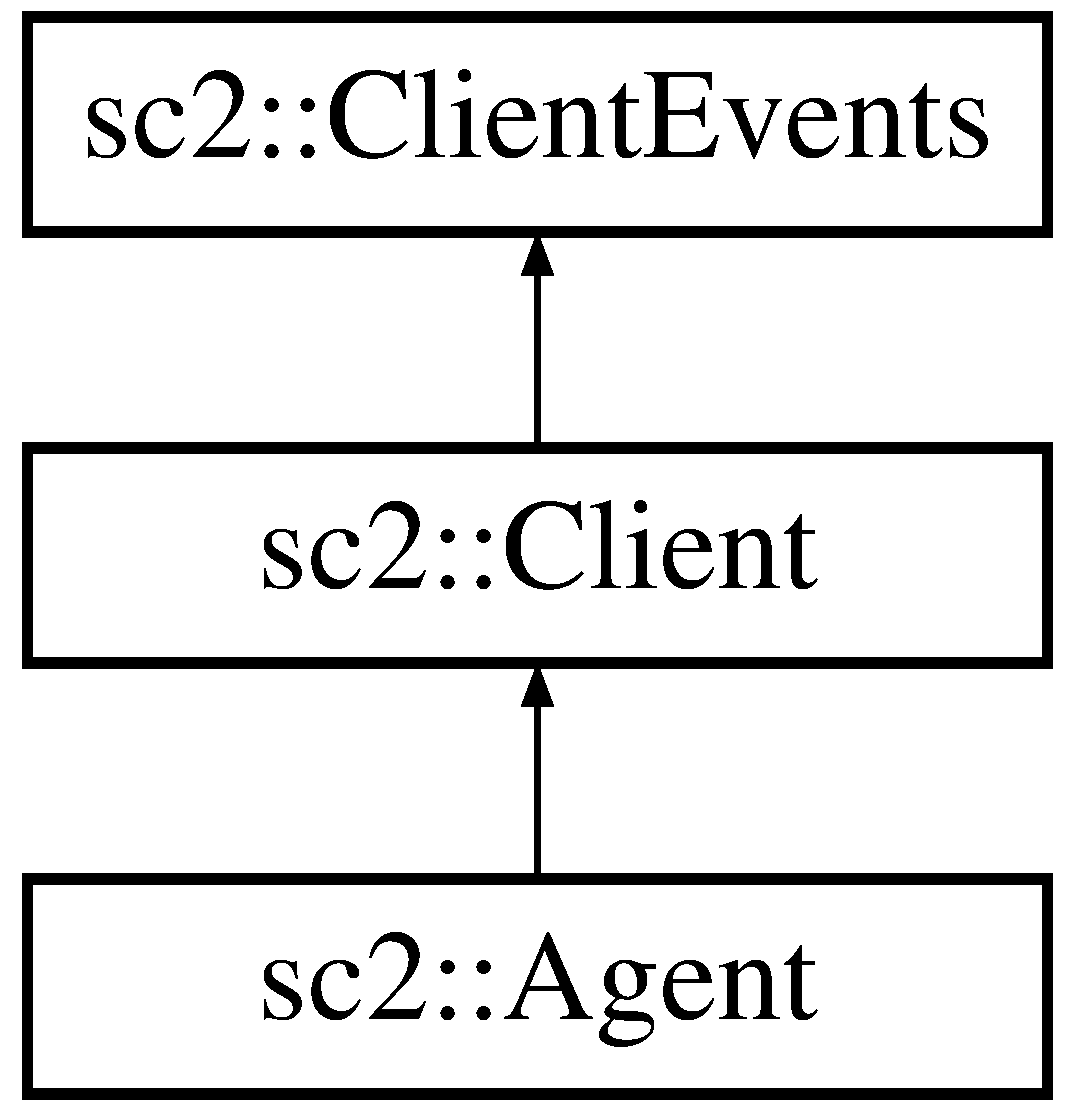
\includegraphics[height=3.000000cm]{classsc2_1_1_agent}
\end{center}
\end{figure}
\subsection*{Public Member Functions}
\begin{DoxyCompactItemize}
\item 
\hyperlink{classsc2_1_1_action_interface}{Action\+Interface} $\ast$ \hyperlink{classsc2_1_1_agent_ac0725513a2164c76857a7d2615a31264}{Actions} ()
\item 
\hyperlink{classsc2_1_1_action_feature_layer_interface}{Action\+Feature\+Layer\+Interface} $\ast$ \hyperlink{classsc2_1_1_agent_a0e267c48e4e41e37dc14185113493cc4}{Actions\+Feature\+Layer} ()
\item 
\hyperlink{classsc2_1_1_agent_control_interface}{Agent\+Control\+Interface} $\ast$ \hyperlink{classsc2_1_1_agent_ad47b7a7383489567360ce1697d5e1675}{Agent\+Control} ()
\end{DoxyCompactItemize}


\subsection{Detailed Description}
The base class for user defined bots. 

\subsection{Member Function Documentation}
\mbox{\Hypertarget{classsc2_1_1_agent_ac0725513a2164c76857a7d2615a31264}\label{classsc2_1_1_agent_ac0725513a2164c76857a7d2615a31264}} 
\index{sc2\+::\+Agent@{sc2\+::\+Agent}!Actions@{Actions}}
\index{Actions@{Actions}!sc2\+::\+Agent@{sc2\+::\+Agent}}
\subsubsection{\texorpdfstring{Actions()}{Actions()}}
{\footnotesize\ttfamily \hyperlink{classsc2_1_1_action_interface}{Action\+Interface}$\ast$ sc2\+::\+Agent\+::\+Actions (\begin{DoxyParamCaption}{ }\end{DoxyParamCaption})}

Interface for issuing actions to units. Actions should be batched via the Unit\+Command functions then eventually dispatched with Send\+Actions. If you are stepping the simulation yourself the Step will automatically call Send\+Actions. If your bot is running in real time you must call Send\+Actions yourself. \begin{DoxyReturn}{Returns}
The raw (basic) action interface. 
\end{DoxyReturn}
\mbox{\Hypertarget{classsc2_1_1_agent_a0e267c48e4e41e37dc14185113493cc4}\label{classsc2_1_1_agent_a0e267c48e4e41e37dc14185113493cc4}} 
\index{sc2\+::\+Agent@{sc2\+::\+Agent}!Actions\+Feature\+Layer@{Actions\+Feature\+Layer}}
\index{Actions\+Feature\+Layer@{Actions\+Feature\+Layer}!sc2\+::\+Agent@{sc2\+::\+Agent}}
\subsubsection{\texorpdfstring{Actions\+Feature\+Layer()}{ActionsFeatureLayer()}}
{\footnotesize\ttfamily \hyperlink{classsc2_1_1_action_feature_layer_interface}{Action\+Feature\+Layer\+Interface}$\ast$ sc2\+::\+Agent\+::\+Actions\+Feature\+Layer (\begin{DoxyParamCaption}{ }\end{DoxyParamCaption})}

Interface for issuing actions in feature layers. \begin{DoxyReturn}{Returns}
The feature layer action interface. 
\end{DoxyReturn}
\mbox{\Hypertarget{classsc2_1_1_agent_ad47b7a7383489567360ce1697d5e1675}\label{classsc2_1_1_agent_ad47b7a7383489567360ce1697d5e1675}} 
\index{sc2\+::\+Agent@{sc2\+::\+Agent}!Agent\+Control@{Agent\+Control}}
\index{Agent\+Control@{Agent\+Control}!sc2\+::\+Agent@{sc2\+::\+Agent}}
\subsubsection{\texorpdfstring{Agent\+Control()}{AgentControl()}}
{\footnotesize\ttfamily \hyperlink{classsc2_1_1_agent_control_interface}{Agent\+Control\+Interface}$\ast$ sc2\+::\+Agent\+::\+Agent\+Control (\begin{DoxyParamCaption}{ }\end{DoxyParamCaption})}

The \hyperlink{classsc2_1_1_agent_control_interface}{Agent\+Control\+Interface} is only currently used for restarting a game. For internal use. \begin{DoxyReturn}{Returns}
The agent control interface. 
\end{DoxyReturn}


The documentation for this class was generated from the following file\+:\begin{DoxyCompactItemize}
\item 
include/sc2api/sc2\+\_\+agent.\+h\end{DoxyCompactItemize}

\hypertarget{classsc2_1_1_agent_control_interface}{}\section{sc2\+:\+:Agent\+Control\+Interface Class Reference}
\label{classsc2_1_1_agent_control_interface}\index{sc2\+::\+Agent\+Control\+Interface@{sc2\+::\+Agent\+Control\+Interface}}
\subsection*{Public Member Functions}
\begin{DoxyCompactItemize}
\item 
\mbox{\Hypertarget{classsc2_1_1_agent_control_interface_aee80a32163dfe91c5aac55e6f00f304d}\label{classsc2_1_1_agent_control_interface_aee80a32163dfe91c5aac55e6f00f304d}} 
virtual bool {\bfseries Restart} ()=0
\end{DoxyCompactItemize}


The documentation for this class was generated from the following file\+:\begin{DoxyCompactItemize}
\item 
include/sc2api/sc2\+\_\+control\+\_\+interfaces.\+h\end{DoxyCompactItemize}

\hypertarget{structsc2_1_1_arg}{}\section{sc2\+:\+:Arg Struct Reference}
\label{structsc2_1_1_arg}\index{sc2\+::\+Arg@{sc2\+::\+Arg}}
\subsection*{Public Attributes}
\begin{DoxyCompactItemize}
\item 
\mbox{\Hypertarget{structsc2_1_1_arg_ac7ee536715c0f89ed6b61365966765bd}\label{structsc2_1_1_arg_ac7ee536715c0f89ed6b61365966765bd}} 
std\+::string {\bfseries abbreviation\+\_\+}
\item 
\mbox{\Hypertarget{structsc2_1_1_arg_a31666378c9bab5f487d7221c8ca500bd}\label{structsc2_1_1_arg_a31666378c9bab5f487d7221c8ca500bd}} 
std\+::string {\bfseries fullname\+\_\+}
\item 
\mbox{\Hypertarget{structsc2_1_1_arg_a31fa9da9f7ec84d7eadab713f38dabcd}\label{structsc2_1_1_arg_a31fa9da9f7ec84d7eadab713f38dabcd}} 
std\+::string {\bfseries description\+\_\+}
\item 
\mbox{\Hypertarget{structsc2_1_1_arg_ac1f3f8a74bebd8192697e45398a4b3e9}\label{structsc2_1_1_arg_ac1f3f8a74bebd8192697e45398a4b3e9}} 
bool {\bfseries required\+\_\+}
\end{DoxyCompactItemize}


The documentation for this struct was generated from the following file\+:\begin{DoxyCompactItemize}
\item 
include/sc2utils/sc2\+\_\+arg\+\_\+parser.\+h\end{DoxyCompactItemize}

\hypertarget{classsc2_1_1_arg_parser}{}\section{sc2\+:\+:Arg\+Parser Class Reference}
\label{classsc2_1_1_arg_parser}\index{sc2\+::\+Arg\+Parser@{sc2\+::\+Arg\+Parser}}
\subsection*{Public Member Functions}
\begin{DoxyCompactItemize}
\item 
\mbox{\Hypertarget{classsc2_1_1_arg_parser_a134a3fa3ddeb9f5218a0530def37164e}\label{classsc2_1_1_arg_parser_a134a3fa3ddeb9f5218a0530def37164e}} 
{\bfseries Arg\+Parser} (const std\+::string \&executable\+\_\+name)
\item 
\mbox{\Hypertarget{classsc2_1_1_arg_parser_aea7d752e4e80bbb0a66c8f39f64ae034}\label{classsc2_1_1_arg_parser_aea7d752e4e80bbb0a66c8f39f64ae034}} 
{\bfseries Arg\+Parser} (const std\+::string \&usage, const std\+::string \&description, const std\+::string \&example=\char`\"{}\char`\"{})
\item 
\mbox{\Hypertarget{classsc2_1_1_arg_parser_a1719a8b54007b11fd47b48187b5cbe1a}\label{classsc2_1_1_arg_parser_a1719a8b54007b11fd47b48187b5cbe1a}} 
void {\bfseries Add\+Options} (const std\+::vector$<$ \hyperlink{structsc2_1_1_arg}{Arg} $>$ \&options)
\item 
\mbox{\Hypertarget{classsc2_1_1_arg_parser_aba7c6ccebaa16fe0407d2174d12786b2}\label{classsc2_1_1_arg_parser_aba7c6ccebaa16fe0407d2174d12786b2}} 
bool {\bfseries Parse} (int argc, char $\ast$argv\mbox{[}$\,$\mbox{]})
\item 
\mbox{\Hypertarget{classsc2_1_1_arg_parser_ac62cf043d391a622144bf6e92f2dc132}\label{classsc2_1_1_arg_parser_ac62cf043d391a622144bf6e92f2dc132}} 
bool {\bfseries Get} (const std\+::string \&identifier, std\+::string \&value)
\item 
\mbox{\Hypertarget{classsc2_1_1_arg_parser_ae0fc51452403ae3d752e6e2d9ede8c66}\label{classsc2_1_1_arg_parser_ae0fc51452403ae3d752e6e2d9ede8c66}} 
void {\bfseries Print\+Help} ()
\item 
\mbox{\Hypertarget{classsc2_1_1_arg_parser_a8043e051d897635526bf542b96a3235c}\label{classsc2_1_1_arg_parser_a8043e051d897635526bf542b96a3235c}} 
void {\bfseries Print\+Usage} ()
\end{DoxyCompactItemize}


The documentation for this class was generated from the following file\+:\begin{DoxyCompactItemize}
\item 
include/sc2utils/sc2\+\_\+arg\+\_\+parser.\+h\end{DoxyCompactItemize}

\hypertarget{structsc2_1_1_available_abilities}{}\section{sc2\+:\+:Available\+Abilities Struct Reference}
\label{structsc2_1_1_available_abilities}\index{sc2\+::\+Available\+Abilities@{sc2\+::\+Available\+Abilities}}


All available abilities for a unit.  




{\ttfamily \#include $<$sc2\+\_\+data.\+h$>$}

\subsection*{Public Member Functions}
\begin{DoxyCompactItemize}
\item 
bool \hyperlink{structsc2_1_1_available_abilities_a9ee95eab5fb81086c452a8790c13c368}{Is\+Valid} () const
\end{DoxyCompactItemize}
\subsection*{Public Attributes}
\begin{DoxyCompactItemize}
\item 
\mbox{\Hypertarget{structsc2_1_1_available_abilities_af894555e7aa8ca9f4a7eb601a898287c}\label{structsc2_1_1_available_abilities_af894555e7aa8ca9f4a7eb601a898287c}} 
std\+::vector$<$ \hyperlink{structsc2_1_1_available_ability}{Available\+Ability} $>$ \hyperlink{structsc2_1_1_available_abilities_af894555e7aa8ca9f4a7eb601a898287c}{abilities}
\begin{DoxyCompactList}\small\item\em The available abilities. \end{DoxyCompactList}\item 
\mbox{\Hypertarget{structsc2_1_1_available_abilities_aa89084e4b2b9948815f833f3ed40a4fb}\label{structsc2_1_1_available_abilities_aa89084e4b2b9948815f833f3ed40a4fb}} 
Tag \hyperlink{structsc2_1_1_available_abilities_aa89084e4b2b9948815f833f3ed40a4fb}{unit\+\_\+tag}
\begin{DoxyCompactList}\small\item\em The unit. \end{DoxyCompactList}\item 
\mbox{\Hypertarget{structsc2_1_1_available_abilities_a731332d717ebab756e47f2fd6d706cb0}\label{structsc2_1_1_available_abilities_a731332d717ebab756e47f2fd6d706cb0}} 
\hyperlink{classsc2_1_1_s_c2_type}{Unit\+Type\+ID} \hyperlink{structsc2_1_1_available_abilities_a731332d717ebab756e47f2fd6d706cb0}{unit\+\_\+type\+\_\+id}
\begin{DoxyCompactList}\small\item\em The unit type. \end{DoxyCompactList}\end{DoxyCompactItemize}


\subsection{Detailed Description}
All available abilities for a unit. 

\subsection{Member Function Documentation}
\mbox{\Hypertarget{structsc2_1_1_available_abilities_a9ee95eab5fb81086c452a8790c13c368}\label{structsc2_1_1_available_abilities_a9ee95eab5fb81086c452a8790c13c368}} 
\index{sc2\+::\+Available\+Abilities@{sc2\+::\+Available\+Abilities}!Is\+Valid@{Is\+Valid}}
\index{Is\+Valid@{Is\+Valid}!sc2\+::\+Available\+Abilities@{sc2\+::\+Available\+Abilities}}
\subsubsection{\texorpdfstring{Is\+Valid()}{IsValid()}}
{\footnotesize\ttfamily bool sc2\+::\+Available\+Abilities\+::\+Is\+Valid (\begin{DoxyParamCaption}{ }\end{DoxyParamCaption}) const\hspace{0.3cm}{\ttfamily [inline]}}

Returns true if this object refers to a valid unit and unit type. \begin{DoxyReturn}{Returns}
If this object is valid. 
\end{DoxyReturn}


The documentation for this struct was generated from the following file\+:\begin{DoxyCompactItemize}
\item 
include/sc2api/sc2\+\_\+data.\+h\end{DoxyCompactItemize}

\hypertarget{structsc2_1_1_available_ability}{}\section{sc2\+:\+:Available\+Ability Struct Reference}
\label{structsc2_1_1_available_ability}\index{sc2\+::\+Available\+Ability@{sc2\+::\+Available\+Ability}}


Indicates if an ability is available, and if that ability requires a point.  




{\ttfamily \#include $<$sc2\+\_\+data.\+h$>$}

\subsection*{Public Member Functions}
\begin{DoxyCompactItemize}
\item 
\mbox{\Hypertarget{structsc2_1_1_available_ability_af99b42b20bdaf45e9f3d4745eb222289}\label{structsc2_1_1_available_ability_af99b42b20bdaf45e9f3d4745eb222289}} 
{\bfseries Available\+Ability} (\hyperlink{classsc2_1_1_s_c2_type}{Ability\+ID} \hyperlink{structsc2_1_1_available_ability_ace0e29a4331fdf570146b3768203f294}{ability\+\_\+id}, bool \hyperlink{structsc2_1_1_available_ability_ac8ec9ad102f838de53565b75c4b67e99}{requires\+\_\+point})
\end{DoxyCompactItemize}
\subsection*{Public Attributes}
\begin{DoxyCompactItemize}
\item 
\mbox{\Hypertarget{structsc2_1_1_available_ability_ace0e29a4331fdf570146b3768203f294}\label{structsc2_1_1_available_ability_ace0e29a4331fdf570146b3768203f294}} 
\hyperlink{classsc2_1_1_s_c2_type}{Ability\+ID} \hyperlink{structsc2_1_1_available_ability_ace0e29a4331fdf570146b3768203f294}{ability\+\_\+id} = 0
\begin{DoxyCompactList}\small\item\em Ability that is available. \end{DoxyCompactList}\item 
\mbox{\Hypertarget{structsc2_1_1_available_ability_ac8ec9ad102f838de53565b75c4b67e99}\label{structsc2_1_1_available_ability_ac8ec9ad102f838de53565b75c4b67e99}} 
bool \hyperlink{structsc2_1_1_available_ability_ac8ec9ad102f838de53565b75c4b67e99}{requires\+\_\+point} = false
\begin{DoxyCompactList}\small\item\em Indicates if the ability requires a point to invoke. \end{DoxyCompactList}\end{DoxyCompactItemize}


\subsection{Detailed Description}
Indicates if an ability is available, and if that ability requires a point. 

The documentation for this struct was generated from the following file\+:\begin{DoxyCompactItemize}
\item 
include/sc2api/sc2\+\_\+data.\+h\end{DoxyCompactItemize}

\hypertarget{structsc2_1_1_buff_data}{}\section{sc2\+:\+:Buff\+Data Struct Reference}
\label{structsc2_1_1_buff_data}\index{sc2\+::\+Buff\+Data@{sc2\+::\+Buff\+Data}}


Buff data.  




{\ttfamily \#include $<$sc2\+\_\+data.\+h$>$}

\subsection*{Public Member Functions}
\begin{DoxyCompactItemize}
\item 
\mbox{\Hypertarget{structsc2_1_1_buff_data_a95a4fae8f7b7ece6fbd9c16ba6bd2b0a}\label{structsc2_1_1_buff_data_a95a4fae8f7b7ece6fbd9c16ba6bd2b0a}} 
void {\bfseries Read\+From\+Proto} (const S\+C2\+A\+P\+I\+Protocol\+::\+Buff\+Data \&buff\+\_\+data)
\item 
\mbox{\Hypertarget{structsc2_1_1_buff_data_acd334464556d30678a2f7aaf43265432}\label{structsc2_1_1_buff_data_acd334464556d30678a2f7aaf43265432}} 
std\+::string {\bfseries Log} () const
\end{DoxyCompactItemize}
\subsection*{Public Attributes}
\begin{DoxyCompactItemize}
\item 
\mbox{\Hypertarget{structsc2_1_1_buff_data_ab5c92fdf01e7eb2d5629df664a99e0bc}\label{structsc2_1_1_buff_data_ab5c92fdf01e7eb2d5629df664a99e0bc}} 
uint32\+\_\+t {\bfseries buff\+\_\+id}
\item 
\mbox{\Hypertarget{structsc2_1_1_buff_data_a8b97134b47f6cbe973fe1eba84bc3612}\label{structsc2_1_1_buff_data_a8b97134b47f6cbe973fe1eba84bc3612}} 
std\+::string {\bfseries name}
\end{DoxyCompactItemize}


\subsection{Detailed Description}
Buff data. 

The documentation for this struct was generated from the following file\+:\begin{DoxyCompactItemize}
\item 
include/sc2api/sc2\+\_\+data.\+h\end{DoxyCompactItemize}

\hypertarget{structsc2_1_1_category_score_details}{}\section{sc2\+:\+:Category\+Score\+Details Struct Reference}
\label{structsc2_1_1_category_score_details}\index{sc2\+::\+Category\+Score\+Details@{sc2\+::\+Category\+Score\+Details}}


\hyperlink{structsc2_1_1_score}{Score} by category.  




{\ttfamily \#include $<$sc2\+\_\+score.\+h$>$}

\subsection*{Static Public Member Functions}
\begin{DoxyCompactItemize}
\item 
\mbox{\Hypertarget{structsc2_1_1_category_score_details_a6afc040055f78a22b24dd0e73e9f5c7f}\label{structsc2_1_1_category_score_details_a6afc040055f78a22b24dd0e73e9f5c7f}} 
static void {\bfseries Add\+Entries} (\hyperlink{structsc2_1_1_score_entry}{Score\+Entry} base, std\+::vector$<$ \hyperlink{structsc2_1_1_score_entry}{Score\+Entry} $>$ \&entries)
\end{DoxyCompactItemize}
\subsection*{Public Attributes}
\begin{DoxyCompactItemize}
\item 
\mbox{\Hypertarget{structsc2_1_1_category_score_details_ab9b21836c95766c6b4a7bf5252af1d96}\label{structsc2_1_1_category_score_details_ab9b21836c95766c6b4a7bf5252af1d96}} 
float {\bfseries none}
\item 
\mbox{\Hypertarget{structsc2_1_1_category_score_details_ab6bfbc156755543869c8fe3752be74d3}\label{structsc2_1_1_category_score_details_ab6bfbc156755543869c8fe3752be74d3}} 
float {\bfseries army}
\item 
\mbox{\Hypertarget{structsc2_1_1_category_score_details_a91b3b9494c31de0d080e7e71d1af9201}\label{structsc2_1_1_category_score_details_a91b3b9494c31de0d080e7e71d1af9201}} 
float {\bfseries economy}
\item 
\mbox{\Hypertarget{structsc2_1_1_category_score_details_aa26c67bfad47a0070a84b3be1b1fb0e5}\label{structsc2_1_1_category_score_details_aa26c67bfad47a0070a84b3be1b1fb0e5}} 
float {\bfseries technology}
\item 
\mbox{\Hypertarget{structsc2_1_1_category_score_details_a2472de45854b42861e0c92b3bbd5f731}\label{structsc2_1_1_category_score_details_a2472de45854b42861e0c92b3bbd5f731}} 
float {\bfseries upgrade}
\end{DoxyCompactItemize}


\subsection{Detailed Description}
\hyperlink{structsc2_1_1_score}{Score} by category. 

The documentation for this struct was generated from the following file\+:\begin{DoxyCompactItemize}
\item 
include/sc2api/\hyperlink{sc2__score_8h}{sc2\+\_\+score.\+h}\end{DoxyCompactItemize}

\hypertarget{classsc2_1_1_client}{}\section{sc2\+:\+:Client Class Reference}
\label{classsc2_1_1_client}\index{sc2\+::\+Client@{sc2\+::\+Client}}


The base class for \hyperlink{classsc2_1_1_agent}{Agent} and \hyperlink{classsc2_1_1_replay_observer}{Replay\+Observer}.  




{\ttfamily \#include $<$sc2\+\_\+client.\+h$>$}

Inheritance diagram for sc2\+:\+:Client\+:\begin{figure}[H]
\begin{center}
\leavevmode
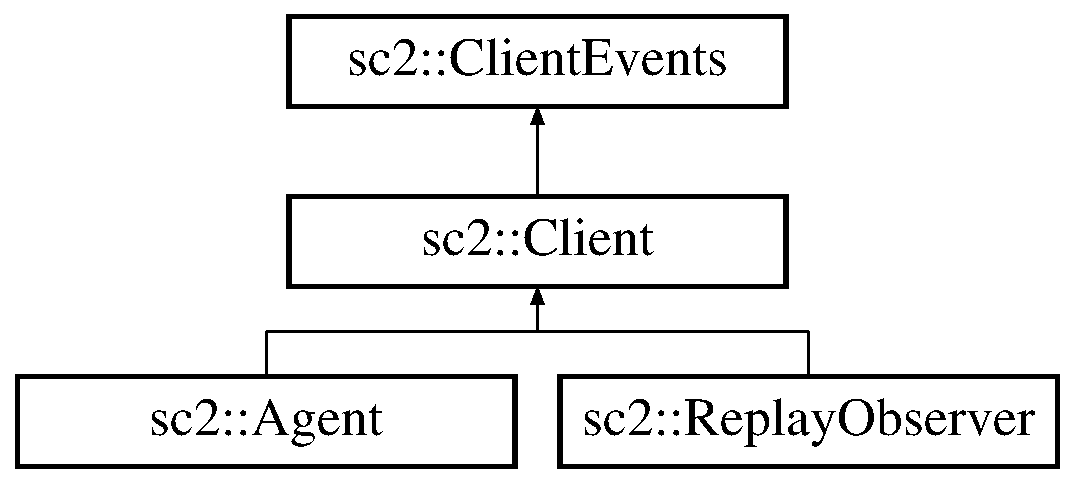
\includegraphics[height=3.000000cm]{classsc2_1_1_client}
\end{center}
\end{figure}
\subsection*{Public Member Functions}
\begin{DoxyCompactItemize}
\item 
\mbox{\Hypertarget{classsc2_1_1_client_a9bde4735245a945f37c5505cde5d09c1}\label{classsc2_1_1_client_a9bde4735245a945f37c5505cde5d09c1}} 
const \hyperlink{classsc2_1_1_observation_interface}{Observation\+Interface} $\ast$ \hyperlink{classsc2_1_1_client_a9bde4735245a945f37c5505cde5d09c1}{Observation} () const
\begin{DoxyCompactList}\small\item\em The \hyperlink{classsc2_1_1_observation_interface}{Observation\+Interface} is used to query game state. \end{DoxyCompactList}\item 
\mbox{\Hypertarget{classsc2_1_1_client_acdc61fe5c58e0a8f4f246d8fbcc5cefc}\label{classsc2_1_1_client_acdc61fe5c58e0a8f4f246d8fbcc5cefc}} 
\hyperlink{classsc2_1_1_query_interface}{Query\+Interface} $\ast$ \hyperlink{classsc2_1_1_client_acdc61fe5c58e0a8f4f246d8fbcc5cefc}{Query} ()
\begin{DoxyCompactList}\small\item\em The Unit\+Query interface is used to issue commands to units. \end{DoxyCompactList}\item 
\mbox{\Hypertarget{classsc2_1_1_client_ac42601e18b7c109f6f0e58a7780a79ac}\label{classsc2_1_1_client_ac42601e18b7c109f6f0e58a7780a79ac}} 
\hyperlink{classsc2_1_1_debug_interface}{Debug\+Interface} $\ast$ \hyperlink{classsc2_1_1_client_ac42601e18b7c109f6f0e58a7780a79ac}{Debug} ()
\begin{DoxyCompactList}\small\item\em The \hyperlink{classsc2_1_1_debug_interface}{Debug\+Interface} allows a derived class to print text, draw primitive shapes and spawn/destroy units. \end{DoxyCompactList}\item 
\hyperlink{classsc2_1_1_control_interface}{Control\+Interface} $\ast$ \hyperlink{classsc2_1_1_client_a741b9dd091f11694dd814c9b01f86dd8}{Control} ()
\item 
\mbox{\Hypertarget{classsc2_1_1_client_a90089d27b898fe537ccee87def3cec4b}\label{classsc2_1_1_client_a90089d27b898fe537ccee87def3cec4b}} 
const \hyperlink{classsc2_1_1_control_interface}{Control\+Interface} $\ast$ {\bfseries Control} () const
\end{DoxyCompactItemize}


\subsection{Detailed Description}
The base class for \hyperlink{classsc2_1_1_agent}{Agent} and \hyperlink{classsc2_1_1_replay_observer}{Replay\+Observer}. 

\subsection{Member Function Documentation}
\mbox{\Hypertarget{classsc2_1_1_client_a741b9dd091f11694dd814c9b01f86dd8}\label{classsc2_1_1_client_a741b9dd091f11694dd814c9b01f86dd8}} 
\index{sc2\+::\+Client@{sc2\+::\+Client}!Control@{Control}}
\index{Control@{Control}!sc2\+::\+Client@{sc2\+::\+Client}}
\subsubsection{\texorpdfstring{Control()}{Control()}}
{\footnotesize\ttfamily \hyperlink{classsc2_1_1_control_interface}{Control\+Interface}$\ast$ sc2\+::\+Client\+::\+Control (\begin{DoxyParamCaption}{ }\end{DoxyParamCaption})}

The \hyperlink{classsc2_1_1_control_interface}{Control\+Interface} is only meant to be used by the coordinator as it provides functionality for connecting to Starcraft2, setting up a websocket connection and issuing blocking commands via S\+C2\textquotesingle{}s protocol. 

The documentation for this class was generated from the following file\+:\begin{DoxyCompactItemize}
\item 
include/sc2api/\hyperlink{sc2__client_8h}{sc2\+\_\+client.\+h}\end{DoxyCompactItemize}

\hypertarget{classsc2_1_1_client_events}{}\section{sc2\+:\+:Client\+Events Class Reference}
\label{classsc2_1_1_client_events}\index{sc2\+::\+Client\+Events@{sc2\+::\+Client\+Events}}


A set of common events a user can override in their derived bot or replay observer class.  




{\ttfamily \#include $<$sc2\+\_\+client.\+h$>$}

Inheritance diagram for sc2\+:\+:Client\+Events\+:\begin{figure}[H]
\begin{center}
\leavevmode
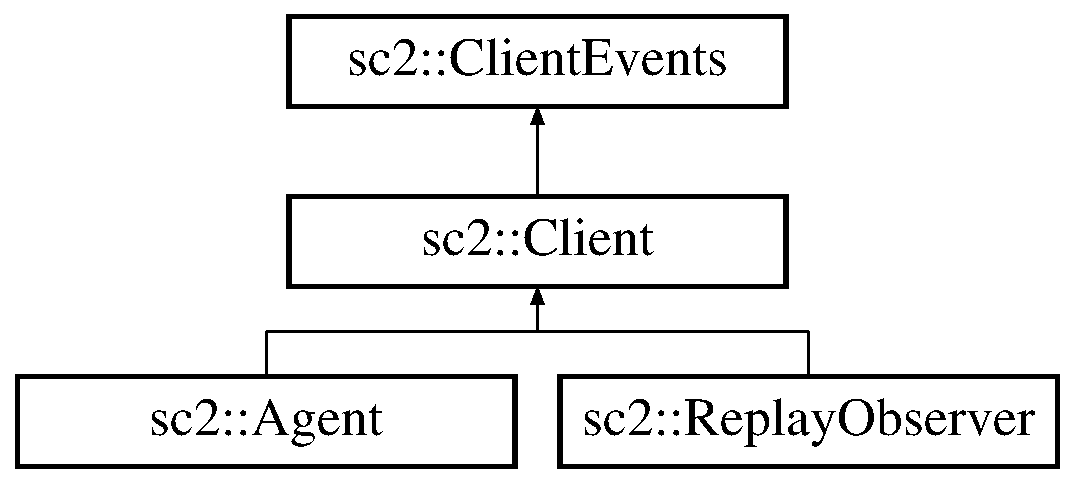
\includegraphics[height=3.000000cm]{classsc2_1_1_client_events}
\end{center}
\end{figure}
\subsection*{Public Member Functions}
\begin{DoxyCompactItemize}
\item 
\mbox{\Hypertarget{classsc2_1_1_client_events_ab980f6942030d3a0cd42e00782742237}\label{classsc2_1_1_client_events_ab980f6942030d3a0cd42e00782742237}} 
virtual void \hyperlink{classsc2_1_1_client_events_ab980f6942030d3a0cd42e00782742237}{On\+Game\+Full\+Start} ()
\begin{DoxyCompactList}\small\item\em Called when a game is started after a load. Fast restarting will not call this. \end{DoxyCompactList}\item 
\mbox{\Hypertarget{classsc2_1_1_client_events_a6e2542b183f6ac980440cc93476163a3}\label{classsc2_1_1_client_events_a6e2542b183f6ac980440cc93476163a3}} 
virtual void \hyperlink{classsc2_1_1_client_events_a6e2542b183f6ac980440cc93476163a3}{On\+Game\+Start} ()
\begin{DoxyCompactList}\small\item\em Called when a game is started or restarted. \end{DoxyCompactList}\item 
\mbox{\Hypertarget{classsc2_1_1_client_events_a2c5023d18ffc88bed76c844e643ef60d}\label{classsc2_1_1_client_events_a2c5023d18ffc88bed76c844e643ef60d}} 
virtual void \hyperlink{classsc2_1_1_client_events_a2c5023d18ffc88bed76c844e643ef60d}{On\+Game\+End} ()
\begin{DoxyCompactList}\small\item\em Called when a game has ended. \end{DoxyCompactList}\item 
virtual void \hyperlink{classsc2_1_1_client_events_a6f5839e220d2a5a19b30065e0b8290c4}{On\+Step} ()
\item 
virtual void \hyperlink{classsc2_1_1_client_events_ae80cd238b975c76b5db062939949b598}{On\+Unit\+Destroyed} (const \hyperlink{classsc2_1_1_unit}{Unit} \&unit)
\item 
virtual void \hyperlink{classsc2_1_1_client_events_a2619e1734feeccd4f8412fd7447fe230}{On\+Unit\+Created} (const \hyperlink{classsc2_1_1_unit}{Unit} \&unit)
\item 
virtual void \hyperlink{classsc2_1_1_client_events_a5d57eb9cdfa579a7c50442305dbf8635}{On\+Unit\+Idle} (const \hyperlink{classsc2_1_1_unit}{Unit} \&unit)
\item 
virtual void \hyperlink{classsc2_1_1_client_events_a0ff0017571ba53e018f85dda03861c3a}{On\+Upgrade\+Completed} (\hyperlink{classsc2_1_1_s_c2_type}{Upgrade\+ID} upgrade)
\item 
virtual void \hyperlink{classsc2_1_1_client_events_a9bf081c662bf5e5e64598f8c05f9a309}{On\+Building\+Construction\+Complete} (const \hyperlink{classsc2_1_1_unit}{Unit} \&unit)
\item 
\mbox{\Hypertarget{classsc2_1_1_client_events_afde152c65ab94bdb57e345a8fd1532aa}\label{classsc2_1_1_client_events_afde152c65ab94bdb57e345a8fd1532aa}} 
virtual void \hyperlink{classsc2_1_1_client_events_afde152c65ab94bdb57e345a8fd1532aa}{On\+Nydus\+Detected} ()
\begin{DoxyCompactList}\small\item\em Called when a nydus is placed. \end{DoxyCompactList}\item 
\mbox{\Hypertarget{classsc2_1_1_client_events_ab9923f256e3bf6e518ccb8ec26f8ae88}\label{classsc2_1_1_client_events_ab9923f256e3bf6e518ccb8ec26f8ae88}} 
virtual void \hyperlink{classsc2_1_1_client_events_ab9923f256e3bf6e518ccb8ec26f8ae88}{On\+Nuclear\+Launch\+Detected} ()
\begin{DoxyCompactList}\small\item\em Called when a nuclear launch is detected. \end{DoxyCompactList}\item 
virtual void \hyperlink{classsc2_1_1_client_events_aecbbd77ffd17a729b307f87bbb899cc9}{On\+Unit\+Enter\+Vision} (const \hyperlink{classsc2_1_1_unit}{Unit} \&unit)
\item 
\mbox{\Hypertarget{classsc2_1_1_client_events_a5205616dd617571eca2b437d8baf257d}\label{classsc2_1_1_client_events_a5205616dd617571eca2b437d8baf257d}} 
virtual void \hyperlink{classsc2_1_1_client_events_a5205616dd617571eca2b437d8baf257d}{On\+Error} (const std\+::vector$<$ \hyperlink{sc2__client_8h_ac7d3e3694a208204e099f04c1e5eded0}{Client\+Error} $>$ \&client\+\_\+errors, const std\+::vector$<$ std\+::string $>$ \&protocol\+\_\+errors=\{\})
\begin{DoxyCompactList}\small\item\em Called for various errors the library can encounter. See Client\+Error enum for possible errors. \end{DoxyCompactList}\end{DoxyCompactItemize}


\subsection{Detailed Description}
A set of common events a user can override in their derived bot or replay observer class. 

\subsection{Member Function Documentation}
\mbox{\Hypertarget{classsc2_1_1_client_events_a9bf081c662bf5e5e64598f8c05f9a309}\label{classsc2_1_1_client_events_a9bf081c662bf5e5e64598f8c05f9a309}} 
\index{sc2\+::\+Client\+Events@{sc2\+::\+Client\+Events}!On\+Building\+Construction\+Complete@{On\+Building\+Construction\+Complete}}
\index{On\+Building\+Construction\+Complete@{On\+Building\+Construction\+Complete}!sc2\+::\+Client\+Events@{sc2\+::\+Client\+Events}}
\subsubsection{\texorpdfstring{On\+Building\+Construction\+Complete()}{OnBuildingConstructionComplete()}}
{\footnotesize\ttfamily virtual void sc2\+::\+Client\+Events\+::\+On\+Building\+Construction\+Complete (\begin{DoxyParamCaption}\item[{const \hyperlink{classsc2_1_1_unit}{Unit} \&}]{unit }\end{DoxyParamCaption})\hspace{0.3cm}{\ttfamily [inline]}, {\ttfamily [virtual]}}

Called when the unit in the previous step had a build progress less than 1.\+0 but is greater than or equal to 1.\+0 in the current step. 
\begin{DoxyParams}{Parameters}
{\em unit} & The constructed unit. \\
\hline
\end{DoxyParams}
\mbox{\Hypertarget{classsc2_1_1_client_events_a6f5839e220d2a5a19b30065e0b8290c4}\label{classsc2_1_1_client_events_a6f5839e220d2a5a19b30065e0b8290c4}} 
\index{sc2\+::\+Client\+Events@{sc2\+::\+Client\+Events}!On\+Step@{On\+Step}}
\index{On\+Step@{On\+Step}!sc2\+::\+Client\+Events@{sc2\+::\+Client\+Events}}
\subsubsection{\texorpdfstring{On\+Step()}{OnStep()}}
{\footnotesize\ttfamily virtual void sc2\+::\+Client\+Events\+::\+On\+Step (\begin{DoxyParamCaption}{ }\end{DoxyParamCaption})\hspace{0.3cm}{\ttfamily [inline]}, {\ttfamily [virtual]}}

This event will only get called when stepping. It will not get called in a real time game. In a real time game the user will be responsible for calling Get\+Observation() via the \hyperlink{classsc2_1_1_observation_interface}{Observation\+Interface}. \mbox{\Hypertarget{classsc2_1_1_client_events_a2619e1734feeccd4f8412fd7447fe230}\label{classsc2_1_1_client_events_a2619e1734feeccd4f8412fd7447fe230}} 
\index{sc2\+::\+Client\+Events@{sc2\+::\+Client\+Events}!On\+Unit\+Created@{On\+Unit\+Created}}
\index{On\+Unit\+Created@{On\+Unit\+Created}!sc2\+::\+Client\+Events@{sc2\+::\+Client\+Events}}
\subsubsection{\texorpdfstring{On\+Unit\+Created()}{OnUnitCreated()}}
{\footnotesize\ttfamily virtual void sc2\+::\+Client\+Events\+::\+On\+Unit\+Created (\begin{DoxyParamCaption}\item[{const \hyperlink{classsc2_1_1_unit}{Unit} \&}]{unit }\end{DoxyParamCaption})\hspace{0.3cm}{\ttfamily [inline]}, {\ttfamily [virtual]}}

Called when a \hyperlink{classsc2_1_1_unit}{Unit} has been created by the player. 
\begin{DoxyParams}{Parameters}
{\em unit} & The created unit. \\
\hline
\end{DoxyParams}
\mbox{\Hypertarget{classsc2_1_1_client_events_ae80cd238b975c76b5db062939949b598}\label{classsc2_1_1_client_events_ae80cd238b975c76b5db062939949b598}} 
\index{sc2\+::\+Client\+Events@{sc2\+::\+Client\+Events}!On\+Unit\+Destroyed@{On\+Unit\+Destroyed}}
\index{On\+Unit\+Destroyed@{On\+Unit\+Destroyed}!sc2\+::\+Client\+Events@{sc2\+::\+Client\+Events}}
\subsubsection{\texorpdfstring{On\+Unit\+Destroyed()}{OnUnitDestroyed()}}
{\footnotesize\ttfamily virtual void sc2\+::\+Client\+Events\+::\+On\+Unit\+Destroyed (\begin{DoxyParamCaption}\item[{const \hyperlink{classsc2_1_1_unit}{Unit} \&}]{unit }\end{DoxyParamCaption})\hspace{0.3cm}{\ttfamily [inline]}, {\ttfamily [virtual]}}

Called whenever one of the player\textquotesingle{}s units has been destroyed. 
\begin{DoxyParams}{Parameters}
{\em unit} & The destroyed unit. \\
\hline
\end{DoxyParams}
\mbox{\Hypertarget{classsc2_1_1_client_events_aecbbd77ffd17a729b307f87bbb899cc9}\label{classsc2_1_1_client_events_aecbbd77ffd17a729b307f87bbb899cc9}} 
\index{sc2\+::\+Client\+Events@{sc2\+::\+Client\+Events}!On\+Unit\+Enter\+Vision@{On\+Unit\+Enter\+Vision}}
\index{On\+Unit\+Enter\+Vision@{On\+Unit\+Enter\+Vision}!sc2\+::\+Client\+Events@{sc2\+::\+Client\+Events}}
\subsubsection{\texorpdfstring{On\+Unit\+Enter\+Vision()}{OnUnitEnterVision()}}
{\footnotesize\ttfamily virtual void sc2\+::\+Client\+Events\+::\+On\+Unit\+Enter\+Vision (\begin{DoxyParamCaption}\item[{const \hyperlink{classsc2_1_1_unit}{Unit} \&}]{unit }\end{DoxyParamCaption})\hspace{0.3cm}{\ttfamily [inline]}, {\ttfamily [virtual]}}

Called when an enemy unit enters vision from out of fog of war. 
\begin{DoxyParams}{Parameters}
{\em unit} & The unit entering vision. \\
\hline
\end{DoxyParams}
\mbox{\Hypertarget{classsc2_1_1_client_events_a5d57eb9cdfa579a7c50442305dbf8635}\label{classsc2_1_1_client_events_a5d57eb9cdfa579a7c50442305dbf8635}} 
\index{sc2\+::\+Client\+Events@{sc2\+::\+Client\+Events}!On\+Unit\+Idle@{On\+Unit\+Idle}}
\index{On\+Unit\+Idle@{On\+Unit\+Idle}!sc2\+::\+Client\+Events@{sc2\+::\+Client\+Events}}
\subsubsection{\texorpdfstring{On\+Unit\+Idle()}{OnUnitIdle()}}
{\footnotesize\ttfamily virtual void sc2\+::\+Client\+Events\+::\+On\+Unit\+Idle (\begin{DoxyParamCaption}\item[{const \hyperlink{classsc2_1_1_unit}{Unit} \&}]{unit }\end{DoxyParamCaption})\hspace{0.3cm}{\ttfamily [inline]}, {\ttfamily [virtual]}}

Called when a unit becomes idle, this will only occur as an event so will only be called when the unit becomes idle and not a second time. Being idle is defined by having orders in the previous step and not currently having orders or if it did not exist in the previous step and now does, a unit being created, for instance, will call both On\+Unit\+Created and On\+Unit\+Idle if it does not have a rally set. 
\begin{DoxyParams}{Parameters}
{\em unit} & The idle unit. \\
\hline
\end{DoxyParams}
\mbox{\Hypertarget{classsc2_1_1_client_events_a0ff0017571ba53e018f85dda03861c3a}\label{classsc2_1_1_client_events_a0ff0017571ba53e018f85dda03861c3a}} 
\index{sc2\+::\+Client\+Events@{sc2\+::\+Client\+Events}!On\+Upgrade\+Completed@{On\+Upgrade\+Completed}}
\index{On\+Upgrade\+Completed@{On\+Upgrade\+Completed}!sc2\+::\+Client\+Events@{sc2\+::\+Client\+Events}}
\subsubsection{\texorpdfstring{On\+Upgrade\+Completed()}{OnUpgradeCompleted()}}
{\footnotesize\ttfamily virtual void sc2\+::\+Client\+Events\+::\+On\+Upgrade\+Completed (\begin{DoxyParamCaption}\item[{\hyperlink{classsc2_1_1_s_c2_type}{Upgrade\+ID}}]{upgrade }\end{DoxyParamCaption})\hspace{0.3cm}{\ttfamily [inline]}, {\ttfamily [virtual]}}

Called when an upgrade is finished, warp gate, ground weapons, baneling speed, etc. 
\begin{DoxyParams}{Parameters}
{\em upgrade} & The completed upgrade. \\
\hline
\end{DoxyParams}


The documentation for this class was generated from the following file\+:\begin{DoxyCompactItemize}
\item 
include/sc2api/\hyperlink{sc2__client_8h}{sc2\+\_\+client.\+h}\end{DoxyCompactItemize}

\hypertarget{structsc2_1_1_color}{}\section{sc2\+:\+:Color Struct Reference}
\label{structsc2_1_1_color}\index{sc2\+::\+Color@{sc2\+::\+Color}}


R\+GB \hyperlink{structsc2_1_1_color}{Color}.  




{\ttfamily \#include $<$sc2\+\_\+common.\+h$>$}

\subsection*{Public Member Functions}
\begin{DoxyCompactItemize}
\item 
\mbox{\Hypertarget{structsc2_1_1_color_a58a800974f0282ba6c0546c066de81d5}\label{structsc2_1_1_color_a58a800974f0282ba6c0546c066de81d5}} 
{\bfseries Color} (uint8\+\_\+t in\+\_\+r, uint8\+\_\+t in\+\_\+g, uint8\+\_\+t in\+\_\+b)
\end{DoxyCompactItemize}
\subsection*{Public Attributes}
\begin{DoxyCompactItemize}
\item 
\mbox{\Hypertarget{structsc2_1_1_color_a93be47b4a56bf06fd75d5f32111e65ca}\label{structsc2_1_1_color_a93be47b4a56bf06fd75d5f32111e65ca}} 
uint8\+\_\+t {\bfseries r}
\item 
\mbox{\Hypertarget{structsc2_1_1_color_a03ec2e00a882699d2db7ee00c4efdcae}\label{structsc2_1_1_color_a03ec2e00a882699d2db7ee00c4efdcae}} 
uint8\+\_\+t {\bfseries g}
\item 
\mbox{\Hypertarget{structsc2_1_1_color_a246688d8f256aa999c2de0f9314970a7}\label{structsc2_1_1_color_a246688d8f256aa999c2de0f9314970a7}} 
uint8\+\_\+t {\bfseries b}
\end{DoxyCompactItemize}


\subsection{Detailed Description}
R\+GB \hyperlink{structsc2_1_1_color}{Color}. 

The documentation for this struct was generated from the following file\+:\begin{DoxyCompactItemize}
\item 
include/sc2api/\hyperlink{sc2__common_8h}{sc2\+\_\+common.\+h}\end{DoxyCompactItemize}

\hypertarget{classsc2_1_1_connection}{}\section{sc2\+:\+:Connection Class Reference}
\label{classsc2_1_1_connection}\index{sc2\+::\+Connection@{sc2\+::\+Connection}}


{\ttfamily \#include $<$sc2\+\_\+connection.\+h$>$}

\subsection*{Public Member Functions}
\begin{DoxyCompactItemize}
\item 
bool \hyperlink{classsc2_1_1_connection_ae2b9a0a28789ac5c6304506cf0bea4b0}{Connect} (const std\+::string \&address, int port, bool verbose=true)
\item 
void \hyperlink{classsc2_1_1_connection_af6bd305434d9efd78a6868749e764749}{Send} (const S\+C2\+A\+P\+I\+Protocol\+::\+Request $\ast$request)
\item 
bool \hyperlink{classsc2_1_1_connection_a383d7968897ccc2e35c2716bb110584f}{Receive} (S\+C2\+A\+P\+I\+Protocol\+::\+Response $\ast$\&response, unsigned int timeout\+\_\+ms)
\item 
void \hyperlink{classsc2_1_1_connection_af2d5cf1aff2fef4d30ddd9ab256419ed}{Pop\+Response} (S\+C2\+A\+P\+I\+Protocol\+::\+Response $\ast$\&response)
\item 
void \hyperlink{classsc2_1_1_connection_a1a3d3c532703e0bf7a88f49ee22aa65e}{Set\+Timeout\+Callback} (std\+::function$<$ void()$>$ callback)
\item 
\mbox{\Hypertarget{classsc2_1_1_connection_a1f2556582badc5f98b349efa17d823cd}\label{classsc2_1_1_connection_a1f2556582badc5f98b349efa17d823cd}} 
void {\bfseries Set\+Connection\+Closed\+Callback} (std\+::function$<$ void()$>$ callback)
\item 
bool \hyperlink{classsc2_1_1_connection_a69ca71e72ab2a0a1bad36fc729fedc02}{Has\+Connection} () const
\item 
bool \hyperlink{classsc2_1_1_connection_a7c06854ac5724952f69fb229a3defcee}{Poll\+Response} ()
\item 
void \hyperlink{classsc2_1_1_connection_aad919078849b1b85b38db8d8d11c8004}{Push\+Response} (S\+C2\+A\+P\+I\+Protocol\+::\+Response $\ast$\&response)
\end{DoxyCompactItemize}
\subsection*{Public Attributes}
\begin{DoxyCompactItemize}
\item 
\mbox{\Hypertarget{classsc2_1_1_connection_abab9f14cde0fe589fc3a1c9588c6607a}\label{classsc2_1_1_connection_abab9f14cde0fe589fc3a1c9588c6607a}} 
std\+::function$<$ void()$>$ \hyperlink{classsc2_1_1_connection_abab9f14cde0fe589fc3a1c9588c6607a}{timeout\+\_\+callback\+\_\+}
\begin{DoxyCompactList}\small\item\em Timeout callback. \end{DoxyCompactList}\item 
\mbox{\Hypertarget{classsc2_1_1_connection_a4df89365bfaec33df14cf9a84f42c938}\label{classsc2_1_1_connection_a4df89365bfaec33df14cf9a84f42c938}} 
std\+::function$<$ void()$>$ \hyperlink{classsc2_1_1_connection_a4df89365bfaec33df14cf9a84f42c938}{connection\+\_\+closed\+\_\+callback\+\_\+}
\begin{DoxyCompactList}\small\item\em Timeout callback. \end{DoxyCompactList}\end{DoxyCompactItemize}


\subsection{Detailed Description}
This class acts as a wrapper around a websocket connection and queue responsible for both sending out and receiving protobuf messages. 

\subsection{Member Function Documentation}
\mbox{\Hypertarget{classsc2_1_1_connection_ae2b9a0a28789ac5c6304506cf0bea4b0}\label{classsc2_1_1_connection_ae2b9a0a28789ac5c6304506cf0bea4b0}} 
\index{sc2\+::\+Connection@{sc2\+::\+Connection}!Connect@{Connect}}
\index{Connect@{Connect}!sc2\+::\+Connection@{sc2\+::\+Connection}}
\subsubsection{\texorpdfstring{Connect()}{Connect()}}
{\footnotesize\ttfamily bool sc2\+::\+Connection\+::\+Connect (\begin{DoxyParamCaption}\item[{const std\+::string \&}]{address,  }\item[{int}]{port,  }\item[{bool}]{verbose = {\ttfamily true} }\end{DoxyParamCaption})}

Connects via websocket on a given address/port. 
\begin{DoxyParams}{Parameters}
{\em address} & The address to connect to, will most commonly be used locally so 127.\+0.\+0.\+1. \\
\hline
{\em port} & The port to connect the, the default for s2api is 9168 unless specified otherwise in settings. \\
\hline
\end{DoxyParams}
\begin{DoxyReturn}{Returns}
Returns true if the connection was successful and false otherwise. 
\end{DoxyReturn}
\mbox{\Hypertarget{classsc2_1_1_connection_a69ca71e72ab2a0a1bad36fc729fedc02}\label{classsc2_1_1_connection_a69ca71e72ab2a0a1bad36fc729fedc02}} 
\index{sc2\+::\+Connection@{sc2\+::\+Connection}!Has\+Connection@{Has\+Connection}}
\index{Has\+Connection@{Has\+Connection}!sc2\+::\+Connection@{sc2\+::\+Connection}}
\subsubsection{\texorpdfstring{Has\+Connection()}{HasConnection()}}
{\footnotesize\ttfamily bool sc2\+::\+Connection\+::\+Has\+Connection (\begin{DoxyParamCaption}{ }\end{DoxyParamCaption}) const}

Whether or not the connection is valid. \begin{DoxyReturn}{Returns}
true if the connection is valid, false otherwise. 
\end{DoxyReturn}
\mbox{\Hypertarget{classsc2_1_1_connection_a7c06854ac5724952f69fb229a3defcee}\label{classsc2_1_1_connection_a7c06854ac5724952f69fb229a3defcee}} 
\index{sc2\+::\+Connection@{sc2\+::\+Connection}!Poll\+Response@{Poll\+Response}}
\index{Poll\+Response@{Poll\+Response}!sc2\+::\+Connection@{sc2\+::\+Connection}}
\subsubsection{\texorpdfstring{Poll\+Response()}{PollResponse()}}
{\footnotesize\ttfamily bool sc2\+::\+Connection\+::\+Poll\+Response (\begin{DoxyParamCaption}{ }\end{DoxyParamCaption})}

Polls the queue in a thread safe way to check if a message has been received. \begin{DoxyReturn}{Returns}
true if there is a response in the queue, false otherwise. 
\end{DoxyReturn}
\mbox{\Hypertarget{classsc2_1_1_connection_af2d5cf1aff2fef4d30ddd9ab256419ed}\label{classsc2_1_1_connection_af2d5cf1aff2fef4d30ddd9ab256419ed}} 
\index{sc2\+::\+Connection@{sc2\+::\+Connection}!Pop\+Response@{Pop\+Response}}
\index{Pop\+Response@{Pop\+Response}!sc2\+::\+Connection@{sc2\+::\+Connection}}
\subsubsection{\texorpdfstring{Pop\+Response()}{PopResponse()}}
{\footnotesize\ttfamily void sc2\+::\+Connection\+::\+Pop\+Response (\begin{DoxyParamCaption}\item[{S\+C2\+A\+P\+I\+Protocol\+::\+Response $\ast$\&}]{response }\end{DoxyParamCaption})}

Pop\+Response is called in the Receive function when a message has been received off of the civetweb thread. Alternatively you could poll for responses with Poll\+Response and consume the message manually with this function. 
\begin{DoxyParams}{Parameters}
{\em response} & The response pointer to be filled out. \\
\hline
\end{DoxyParams}
\mbox{\Hypertarget{classsc2_1_1_connection_aad919078849b1b85b38db8d8d11c8004}\label{classsc2_1_1_connection_aad919078849b1b85b38db8d8d11c8004}} 
\index{sc2\+::\+Connection@{sc2\+::\+Connection}!Push\+Response@{Push\+Response}}
\index{Push\+Response@{Push\+Response}!sc2\+::\+Connection@{sc2\+::\+Connection}}
\subsubsection{\texorpdfstring{Push\+Response()}{PushResponse()}}
{\footnotesize\ttfamily void sc2\+::\+Connection\+::\+Push\+Response (\begin{DoxyParamCaption}\item[{S\+C2\+A\+P\+I\+Protocol\+::\+Response $\ast$\&}]{response }\end{DoxyParamCaption})}

Push\+Response is called by a civetweb thread when it receives a message off the socket. Pushing a response triggers a condition and enqueues a message. The condition will cause anyone currently blocking for a response (if Receive is called) to wake up and be able to consume that message. 
\begin{DoxyParams}{Parameters}
{\em response} & A pointer to the Response to queue. \\
\hline
\end{DoxyParams}
\mbox{\Hypertarget{classsc2_1_1_connection_a383d7968897ccc2e35c2716bb110584f}\label{classsc2_1_1_connection_a383d7968897ccc2e35c2716bb110584f}} 
\index{sc2\+::\+Connection@{sc2\+::\+Connection}!Receive@{Receive}}
\index{Receive@{Receive}!sc2\+::\+Connection@{sc2\+::\+Connection}}
\subsubsection{\texorpdfstring{Receive()}{Receive()}}
{\footnotesize\ttfamily bool sc2\+::\+Connection\+::\+Receive (\begin{DoxyParamCaption}\item[{S\+C2\+A\+P\+I\+Protocol\+::\+Response $\ast$\&}]{response,  }\item[{unsigned int}]{timeout\+\_\+ms }\end{DoxyParamCaption})}

Receive will block until a message is received from its websocket connection. If a message is not received within the timeout it will set response to null and return false, it also calls a timeout callback that can be used if a user has any timeout logic. 
\begin{DoxyParams}{Parameters}
{\em response} & The response pointer to be filled out.  The max time, in milliseconds, the function will wait to receive a message. \\
\hline
\end{DoxyParams}
\begin{DoxyReturn}{Returns}
Returns true if a message is received, false otherwise. 
\end{DoxyReturn}
\mbox{\Hypertarget{classsc2_1_1_connection_af6bd305434d9efd78a6868749e764749}\label{classsc2_1_1_connection_af6bd305434d9efd78a6868749e764749}} 
\index{sc2\+::\+Connection@{sc2\+::\+Connection}!Send@{Send}}
\index{Send@{Send}!sc2\+::\+Connection@{sc2\+::\+Connection}}
\subsubsection{\texorpdfstring{Send()}{Send()}}
{\footnotesize\ttfamily void sc2\+::\+Connection\+::\+Send (\begin{DoxyParamCaption}\item[{const S\+C2\+A\+P\+I\+Protocol\+::\+Request $\ast$}]{request }\end{DoxyParamCaption})}

Sends a request via the websocket connection. This function assumes Connect has been called and returned success. It will assert in debug if that\textquotesingle{}s not the case and will early out in a build that doesn\textquotesingle{}t have asserts built in. This function also allocates a byte buffer to accommodate the request, it frees that buffer before returning. 
\begin{DoxyParams}{Parameters}
{\em request} & A pointer to the Request object. \\
\hline
\end{DoxyParams}
\mbox{\Hypertarget{classsc2_1_1_connection_a1a3d3c532703e0bf7a88f49ee22aa65e}\label{classsc2_1_1_connection_a1a3d3c532703e0bf7a88f49ee22aa65e}} 
\index{sc2\+::\+Connection@{sc2\+::\+Connection}!Set\+Timeout\+Callback@{Set\+Timeout\+Callback}}
\index{Set\+Timeout\+Callback@{Set\+Timeout\+Callback}!sc2\+::\+Connection@{sc2\+::\+Connection}}
\subsubsection{\texorpdfstring{Set\+Timeout\+Callback()}{SetTimeoutCallback()}}
{\footnotesize\ttfamily void sc2\+::\+Connection\+::\+Set\+Timeout\+Callback (\begin{DoxyParamCaption}\item[{std\+::function$<$ void()$>$}]{callback }\end{DoxyParamCaption})}

An accessor function that a user can bind a timeout function to. 
\begin{DoxyParams}{Parameters}
{\em callback} & A functor or lambda that represents the callback. \\
\hline
\end{DoxyParams}


The documentation for this class was generated from the following file\+:\begin{DoxyCompactItemize}
\item 
include/sc2api/\hyperlink{sc2__connection_8h}{sc2\+\_\+connection.\+h}\end{DoxyCompactItemize}

\hypertarget{classsc2_1_1_control_interface}{}\section{sc2\+:\+:Control\+Interface Class Reference}
\label{classsc2_1_1_control_interface}\index{sc2\+::\+Control\+Interface@{sc2\+::\+Control\+Interface}}
\subsection*{Public Member Functions}
\begin{DoxyCompactItemize}
\item 
\mbox{\Hypertarget{classsc2_1_1_control_interface_ab90c8107014b8da21ba1d88fdb35aada}\label{classsc2_1_1_control_interface_ab90c8107014b8da21ba1d88fdb35aada}} 
virtual \hyperlink{classsc2_1_1_proto_interface}{Proto\+Interface} \& {\bfseries Proto} ()=0
\item 
\mbox{\Hypertarget{classsc2_1_1_control_interface_a2e8bb94501a1772bfd98f8feb45180d4}\label{classsc2_1_1_control_interface_a2e8bb94501a1772bfd98f8feb45180d4}} 
virtual bool {\bfseries Connect} (const std\+::string \&address, int port, int timeout\+\_\+ms)=0
\item 
\mbox{\Hypertarget{classsc2_1_1_control_interface_afc307e6dc47a1cbbeb47055b199fe3e1}\label{classsc2_1_1_control_interface_afc307e6dc47a1cbbeb47055b199fe3e1}} 
virtual bool {\bfseries Remote\+Save\+Map} (const void $\ast$data, int data\+\_\+size, std\+::string remote\+\_\+path)=0
\item 
\mbox{\Hypertarget{classsc2_1_1_control_interface_a4cd74e4ecacb4fad4aa35b749fd03863}\label{classsc2_1_1_control_interface_a4cd74e4ecacb4fad4aa35b749fd03863}} 
virtual bool {\bfseries Create\+Game} (const std\+::string \&map\+\_\+path, const std\+::vector$<$ \hyperlink{structsc2_1_1_player_setup}{Player\+Setup} $>$ \&players, bool realtime)=0
\item 
\mbox{\Hypertarget{classsc2_1_1_control_interface_a4a2e65b28281bfc5024a62f1a4fba99e}\label{classsc2_1_1_control_interface_a4a2e65b28281bfc5024a62f1a4fba99e}} 
virtual bool {\bfseries Request\+Join\+Game} (\hyperlink{structsc2_1_1_player_setup}{Player\+Setup} setup, const \hyperlink{structsc2_1_1_interface_settings}{Interface\+Settings} \&settings, const \hyperlink{structsc2_1_1_ports}{Ports} \&ports=\hyperlink{structsc2_1_1_ports}{Ports}())=0
\item 
\mbox{\Hypertarget{classsc2_1_1_control_interface_adddde8ba93c8a71d3af5cf38e83e7e9e}\label{classsc2_1_1_control_interface_adddde8ba93c8a71d3af5cf38e83e7e9e}} 
virtual bool {\bfseries Wait\+Join\+Game} ()=0
\item 
\mbox{\Hypertarget{classsc2_1_1_control_interface_ab4fbb92be4e178ab662770155c7b0cd0}\label{classsc2_1_1_control_interface_ab4fbb92be4e178ab662770155c7b0cd0}} 
virtual bool {\bfseries Request\+Leave\+Game} ()=0
\item 
\mbox{\Hypertarget{classsc2_1_1_control_interface_a9858c7bc4cf9485e958d96e518bd5268}\label{classsc2_1_1_control_interface_a9858c7bc4cf9485e958d96e518bd5268}} 
virtual bool {\bfseries Poll\+Leave\+Game} ()=0
\item 
\mbox{\Hypertarget{classsc2_1_1_control_interface_ac4051c302ac0aff7892b7b3dac834bff}\label{classsc2_1_1_control_interface_ac4051c302ac0aff7892b7b3dac834bff}} 
virtual bool {\bfseries Step} (int count=1)=0
\item 
\mbox{\Hypertarget{classsc2_1_1_control_interface_afdceac1202a0160a4bb8bcea6ab227c1}\label{classsc2_1_1_control_interface_afdceac1202a0160a4bb8bcea6ab227c1}} 
virtual bool {\bfseries Wait\+Step} ()=0
\item 
\mbox{\Hypertarget{classsc2_1_1_control_interface_a3e9f1c13939a03abccfc73191cc7fdcf}\label{classsc2_1_1_control_interface_a3e9f1c13939a03abccfc73191cc7fdcf}} 
virtual bool {\bfseries Save\+Replay} (const std\+::string \&path)=0
\item 
\mbox{\Hypertarget{classsc2_1_1_control_interface_a98c730f6414edaa5166890dede1fe83c}\label{classsc2_1_1_control_interface_a98c730f6414edaa5166890dede1fe83c}} 
virtual bool {\bfseries Ping} ()=0
\item 
\mbox{\Hypertarget{classsc2_1_1_control_interface_a02fe1bf89ffb788392bf7707ba9fc049}\label{classsc2_1_1_control_interface_a02fe1bf89ffb788392bf7707ba9fc049}} 
virtual Game\+Response\+Ptr {\bfseries Wait\+For\+Response} ()=0
\item 
\mbox{\Hypertarget{classsc2_1_1_control_interface_a869db0749b2f5db41731886cc7fe9d87}\label{classsc2_1_1_control_interface_a869db0749b2f5db41731886cc7fe9d87}} 
virtual void {\bfseries Set\+Process\+Info} (const \hyperlink{structsc2_1_1_process_info}{Process\+Info} \&pi)=0
\item 
\mbox{\Hypertarget{classsc2_1_1_control_interface_a0c3749bc57d64e1d37f37f0d3d16ec62}\label{classsc2_1_1_control_interface_a0c3749bc57d64e1d37f37f0d3d16ec62}} 
virtual const \hyperlink{structsc2_1_1_process_info}{Process\+Info} \& {\bfseries Get\+Process\+Info} ()=0
\item 
\mbox{\Hypertarget{classsc2_1_1_control_interface_a7856754a90ef19fce1c37d532940cc70}\label{classsc2_1_1_control_interface_a7856754a90ef19fce1c37d532940cc70}} 
virtual App\+State {\bfseries Get\+App\+State} () const =0
\item 
\mbox{\Hypertarget{classsc2_1_1_control_interface_a9cb258851dc5ab3ac7abe7bd817c9531}\label{classsc2_1_1_control_interface_a9cb258851dc5ab3ac7abe7bd817c9531}} 
virtual S\+C2\+A\+P\+I\+Protocol\+::\+Status {\bfseries Get\+Last\+Status} () const =0
\item 
\mbox{\Hypertarget{classsc2_1_1_control_interface_a334adf0a34284e32833554fa189d9746}\label{classsc2_1_1_control_interface_a334adf0a34284e32833554fa189d9746}} 
virtual bool {\bfseries Is\+In\+Game} () const =0
\item 
\mbox{\Hypertarget{classsc2_1_1_control_interface_a8b00eb5fe681665c39855cc3b481ed92}\label{classsc2_1_1_control_interface_a8b00eb5fe681665c39855cc3b481ed92}} 
virtual bool {\bfseries Is\+Finished\+Game} () const =0
\item 
\mbox{\Hypertarget{classsc2_1_1_control_interface_a4bc92e6d97dbe3bd91c93bdf4a450155}\label{classsc2_1_1_control_interface_a4bc92e6d97dbe3bd91c93bdf4a450155}} 
virtual bool {\bfseries Is\+Ready\+For\+Create\+Game} () const =0
\item 
\mbox{\Hypertarget{classsc2_1_1_control_interface_a470cbcfd519ee228c024a9b59a9bbb74}\label{classsc2_1_1_control_interface_a470cbcfd519ee228c024a9b59a9bbb74}} 
virtual bool {\bfseries Has\+Response\+Pending} () const =0
\item 
\mbox{\Hypertarget{classsc2_1_1_control_interface_a4c66296192ffa3e1ba8c3ad2a17d8380}\label{classsc2_1_1_control_interface_a4c66296192ffa3e1ba8c3ad2a17d8380}} 
virtual bool {\bfseries Get\+Observation} ()=0
\item 
\mbox{\Hypertarget{classsc2_1_1_control_interface_aa6f27ad05d20d610c2d4e5b70fc68b49}\label{classsc2_1_1_control_interface_aa6f27ad05d20d610c2d4e5b70fc68b49}} 
virtual bool {\bfseries Poll\+Response} ()=0
\item 
\mbox{\Hypertarget{classsc2_1_1_control_interface_aa8bb71f36fd5106eb21bbceb1ecedf4d}\label{classsc2_1_1_control_interface_aa8bb71f36fd5106eb21bbceb1ecedf4d}} 
virtual bool {\bfseries Consume\+Response} ()=0
\item 
\mbox{\Hypertarget{classsc2_1_1_control_interface_a03c1b68afb1521abf804d2a120f91880}\label{classsc2_1_1_control_interface_a03c1b68afb1521abf804d2a120f91880}} 
virtual bool {\bfseries Issue\+Events} (const std\+::vector$<$ Tag $>$ \&commands=\{\})=0
\item 
\mbox{\Hypertarget{classsc2_1_1_control_interface_a251ee28b1676960c086dc748c52723a3}\label{classsc2_1_1_control_interface_a251ee28b1676960c086dc748c52723a3}} 
virtual void {\bfseries On\+Game\+Start} ()=0
\item 
\mbox{\Hypertarget{classsc2_1_1_control_interface_aac30977133be8ffe2a749a920149b5d3}\label{classsc2_1_1_control_interface_aac30977133be8ffe2a749a920149b5d3}} 
virtual void {\bfseries Dump\+Proto\+Usage} ()=0
\item 
\mbox{\Hypertarget{classsc2_1_1_control_interface_ab3e7b964d0f7e90cc239e5997b09b5c4}\label{classsc2_1_1_control_interface_ab3e7b964d0f7e90cc239e5997b09b5c4}} 
virtual void {\bfseries Error} (\hyperlink{sc2__client_8h_ac7d3e3694a208204e099f04c1e5eded0}{Client\+Error} error, const std\+::vector$<$ std\+::string $>$ \&errors=\{\})=0
\item 
\mbox{\Hypertarget{classsc2_1_1_control_interface_a0f3a503c5e2ed951eed1774866a0280f}\label{classsc2_1_1_control_interface_a0f3a503c5e2ed951eed1774866a0280f}} 
virtual void {\bfseries Error\+If} (bool condition, \hyperlink{sc2__client_8h_ac7d3e3694a208204e099f04c1e5eded0}{Client\+Error} error, const std\+::vector$<$ std\+::string $>$ \&errors=\{\})=0
\item 
\mbox{\Hypertarget{classsc2_1_1_control_interface_ac033fdc8fb4d4aa50a174b6d8870a143}\label{classsc2_1_1_control_interface_ac033fdc8fb4d4aa50a174b6d8870a143}} 
virtual const std\+::vector$<$ \hyperlink{sc2__client_8h_ac7d3e3694a208204e099f04c1e5eded0}{Client\+Error} $>$ \& {\bfseries Get\+Client\+Errors} () const =0
\item 
\mbox{\Hypertarget{classsc2_1_1_control_interface_ac26497e85a0dc55ae82270f0f50d5f03}\label{classsc2_1_1_control_interface_ac26497e85a0dc55ae82270f0f50d5f03}} 
virtual const std\+::vector$<$ std\+::string $>$ \& {\bfseries Get\+Protocol\+Errors} () const =0
\end{DoxyCompactItemize}


The documentation for this class was generated from the following file\+:\begin{DoxyCompactItemize}
\item 
include/sc2api/sc2\+\_\+control\+\_\+interfaces.\+h\end{DoxyCompactItemize}

\hypertarget{classsc2_1_1_coordinator}{}\section{sc2\+:\+:Coordinator Class Reference}
\label{classsc2_1_1_coordinator}\index{sc2\+::\+Coordinator@{sc2\+::\+Coordinator}}


\hyperlink{classsc2_1_1_coordinator}{Coordinator} of one or more clients. Used to start, step and stop games and replays.  




{\ttfamily \#include $<$sc2\+\_\+coordinator.\+h$>$}

\subsection*{Public Member Functions}
\begin{DoxyCompactItemize}
\item 
bool \hyperlink{classsc2_1_1_coordinator_ada059b9a60d901be047ef33ce612c5d2}{Load\+Settings} (int argc, char $\ast$$\ast$argv)
\item 
void \hyperlink{classsc2_1_1_coordinator_a555587bc85ac437711d15b569c75181a}{Set\+Multithreaded} (bool value)
\item 
void \hyperlink{classsc2_1_1_coordinator_a602e6ead93e360771ce36d6ac782fc2a}{Set\+Realtime} (bool value)
\item 
void \hyperlink{classsc2_1_1_coordinator_a7cea718f571effbe25b771315628c685}{Set\+Step\+Size} (int step\+\_\+size)
\item 
void \hyperlink{classsc2_1_1_coordinator_ad906656238e13a8bab21c46f50aecc3d}{Set\+Process\+Path} (const std\+::string \&path)
\item 
void \hyperlink{classsc2_1_1_coordinator_aadbfd927d66314a4eb949b2de2ae37b4}{Set\+Timeout\+MS} (uint32\+\_\+t timeout\+\_\+ms=k\+Default\+Proto\+Interface\+Timeout)
\item 
void \hyperlink{classsc2_1_1_coordinator_aaad48921bac2f4f84471de5e9cff75d5}{Set\+Port\+Start} (int port\+\_\+start)
\item 
void \hyperlink{classsc2_1_1_coordinator_ab46aec5712f6ec8ef12b03854f6e0495}{Set\+Feature\+Layers} (const \hyperlink{structsc2_1_1_feature_layer_settings}{Feature\+Layer\+Settings} \&settings)
\item 
void \hyperlink{classsc2_1_1_coordinator_ace8a0630c6b61d28e81c94bbebad3d7d}{Set\+Render} (const \hyperlink{structsc2_1_1_render_settings}{Render\+Settings} \&settings)
\item 
void \hyperlink{classsc2_1_1_coordinator_a9b0eca71a6f7575f35d1dd5c3e5d73cf}{Set\+Window\+Size} (int width, int height)
\item 
void \hyperlink{classsc2_1_1_coordinator_a6e372788e11c3916fdf1982eb2e55511}{Set\+Window\+Location} (int x, int y)
\item 
\mbox{\Hypertarget{classsc2_1_1_coordinator_aa59950d8ccb9d010288df3e1e6045eb9}\label{classsc2_1_1_coordinator_aa59950d8ccb9d010288df3e1e6045eb9}} 
void \hyperlink{classsc2_1_1_coordinator_aa59950d8ccb9d010288df3e1e6045eb9}{Add\+Command\+Line} (const std\+::string \&option)
\begin{DoxyCompactList}\small\item\em Appends a command line argument to be fed to Star\+Craft II when starting. \end{DoxyCompactList}\item 
\mbox{\Hypertarget{classsc2_1_1_coordinator_aed4bf1a5cf1519fc0488bc5d4641a582}\label{classsc2_1_1_coordinator_aed4bf1a5cf1519fc0488bc5d4641a582}} 
void \hyperlink{classsc2_1_1_coordinator_aed4bf1a5cf1519fc0488bc5d4641a582}{Set\+Participants} (const std\+::vector$<$ \hyperlink{structsc2_1_1_player_setup}{Player\+Setup} $>$ \&participants)
\begin{DoxyCompactList}\small\item\em Sets up the bots and whether they are controlled by in-\/built AI, human or a custom bot. \end{DoxyCompactList}\item 
\mbox{\Hypertarget{classsc2_1_1_coordinator_a16ebfba44b1abbc303770e4958922d05}\label{classsc2_1_1_coordinator_a16ebfba44b1abbc303770e4958922d05}} 
void \hyperlink{classsc2_1_1_coordinator_a16ebfba44b1abbc303770e4958922d05}{Add\+Replay\+Observer} (\hyperlink{classsc2_1_1_replay_observer}{Replay\+Observer} $\ast$replay\+\_\+observer)
\begin{DoxyCompactList}\small\item\em Add an instance of \hyperlink{classsc2_1_1_replay_observer}{Replay\+Observer}, each \hyperlink{classsc2_1_1_replay_observer}{Replay\+Observer} will run a separate Star\+Craft II client. \end{DoxyCompactList}\item 
\mbox{\Hypertarget{classsc2_1_1_coordinator_ac06566447119abac229fd671d39ff2ee}\label{classsc2_1_1_coordinator_ac06566447119abac229fd671d39ff2ee}} 
void \hyperlink{classsc2_1_1_coordinator_ac06566447119abac229fd671d39ff2ee}{Launch\+Starcraft} ()
\begin{DoxyCompactList}\small\item\em Uses settings gathered from Load\+Settings, specifically the path to the executable, to run Star\+Craft II. \end{DoxyCompactList}\item 
void \hyperlink{classsc2_1_1_coordinator_a63fe152548d28b619a7bc577544fcdc8}{Start\+Game} (const std\+::string \&map\+\_\+path=std\+::string())
\item 
bool \hyperlink{classsc2_1_1_coordinator_af70ba5246f9d447eb8a69cd76d364eee}{Update} ()
\item 
\mbox{\Hypertarget{classsc2_1_1_coordinator_af8ae051962776e946e457791f70bf6d2}\label{classsc2_1_1_coordinator_af8ae051962776e946e457791f70bf6d2}} 
void \hyperlink{classsc2_1_1_coordinator_af8ae051962776e946e457791f70bf6d2}{Leave\+Game} ()
\begin{DoxyCompactList}\small\item\em Requests for the currently running game to end. \end{DoxyCompactList}\item 
\mbox{\Hypertarget{classsc2_1_1_coordinator_a31058950f418aa5d488fbda684c02146}\label{classsc2_1_1_coordinator_a31058950f418aa5d488fbda684c02146}} 
bool \hyperlink{classsc2_1_1_coordinator_a31058950f418aa5d488fbda684c02146}{All\+Games\+Ended} () const
\begin{DoxyCompactList}\small\item\em Returns true if all running games have ended. \end{DoxyCompactList}\item 
\mbox{\Hypertarget{classsc2_1_1_coordinator_a86987e853e780259867996f4350e3a87}\label{classsc2_1_1_coordinator_a86987e853e780259867996f4350e3a87}} 
bool \hyperlink{classsc2_1_1_coordinator_a86987e853e780259867996f4350e3a87}{Set\+Replay\+Path} (const std\+::string \&path)
\begin{DoxyCompactList}\small\item\em Sets the path for to a folder of replays to analyze. \end{DoxyCompactList}\item 
\mbox{\Hypertarget{classsc2_1_1_coordinator_a4c4f1b394633b6379aa65bfc264d6f74}\label{classsc2_1_1_coordinator_a4c4f1b394633b6379aa65bfc264d6f74}} 
bool \hyperlink{classsc2_1_1_coordinator_a4c4f1b394633b6379aa65bfc264d6f74}{Load\+Replay\+List} (const std\+::string \&file\+\_\+path)
\begin{DoxyCompactList}\small\item\em Loads replays from a file. \end{DoxyCompactList}\item 
\mbox{\Hypertarget{classsc2_1_1_coordinator_a063c9a9f2d31bc48fb2d4db0aaa7d791}\label{classsc2_1_1_coordinator_a063c9a9f2d31bc48fb2d4db0aaa7d791}} 
void \hyperlink{classsc2_1_1_coordinator_a063c9a9f2d31bc48fb2d4db0aaa7d791}{Save\+Replay\+List} (const std\+::string \&file\+\_\+path)
\begin{DoxyCompactList}\small\item\em Saves replays to a file. \end{DoxyCompactList}\item 
bool \hyperlink{classsc2_1_1_coordinator_a451a422eb904f69b55b273ddfe3f0e58}{Has\+Replays} () const
\item 
\mbox{\Hypertarget{classsc2_1_1_coordinator_a177f926215050e4d249df208b03a387d}\label{classsc2_1_1_coordinator_a177f926215050e4d249df208b03a387d}} 
void \hyperlink{classsc2_1_1_coordinator_a177f926215050e4d249df208b03a387d}{Wait\+For\+All\+Responses} ()
\begin{DoxyCompactList}\small\item\em Blocks for all bots to receive any pending responses. \end{DoxyCompactList}\item 
bool \hyperlink{classsc2_1_1_coordinator_abddb83c4a267e3592932da7d198a97d5}{Remote\+Save\+Map} (const void $\ast$data, int data\+\_\+size, std\+::string remote\+\_\+path)
\begin{DoxyCompactList}\small\item\em Saves a binary blob as a map to a remote location. \end{DoxyCompactList}\item 
std\+::string \hyperlink{classsc2_1_1_coordinator_a9f256d8cc391acd89a29e4369112d69b}{Get\+Exe\+Path} () const
\end{DoxyCompactItemize}


\subsection{Detailed Description}
\hyperlink{classsc2_1_1_coordinator}{Coordinator} of one or more clients. Used to start, step and stop games and replays. 

\subsection{Member Function Documentation}
\mbox{\Hypertarget{classsc2_1_1_coordinator_a9f256d8cc391acd89a29e4369112d69b}\label{classsc2_1_1_coordinator_a9f256d8cc391acd89a29e4369112d69b}} 
\index{sc2\+::\+Coordinator@{sc2\+::\+Coordinator}!Get\+Exe\+Path@{Get\+Exe\+Path}}
\index{Get\+Exe\+Path@{Get\+Exe\+Path}!sc2\+::\+Coordinator@{sc2\+::\+Coordinator}}
\subsubsection{\texorpdfstring{Get\+Exe\+Path()}{GetExePath()}}
{\footnotesize\ttfamily std\+::string sc2\+::\+Coordinator\+::\+Get\+Exe\+Path (\begin{DoxyParamCaption}{ }\end{DoxyParamCaption}) const}

Gets the game executable path. \begin{DoxyReturn}{Returns}
The game executable path. 
\end{DoxyReturn}
\mbox{\Hypertarget{classsc2_1_1_coordinator_a451a422eb904f69b55b273ddfe3f0e58}\label{classsc2_1_1_coordinator_a451a422eb904f69b55b273ddfe3f0e58}} 
\index{sc2\+::\+Coordinator@{sc2\+::\+Coordinator}!Has\+Replays@{Has\+Replays}}
\index{Has\+Replays@{Has\+Replays}!sc2\+::\+Coordinator@{sc2\+::\+Coordinator}}
\subsubsection{\texorpdfstring{Has\+Replays()}{HasReplays()}}
{\footnotesize\ttfamily bool sc2\+::\+Coordinator\+::\+Has\+Replays (\begin{DoxyParamCaption}{ }\end{DoxyParamCaption}) const}

Determines if there are unprocessed replays. \begin{DoxyReturn}{Returns}
Is true if there are replays left. 
\end{DoxyReturn}
\mbox{\Hypertarget{classsc2_1_1_coordinator_ada059b9a60d901be047ef33ce612c5d2}\label{classsc2_1_1_coordinator_ada059b9a60d901be047ef33ce612c5d2}} 
\index{sc2\+::\+Coordinator@{sc2\+::\+Coordinator}!Load\+Settings@{Load\+Settings}}
\index{Load\+Settings@{Load\+Settings}!sc2\+::\+Coordinator@{sc2\+::\+Coordinator}}
\subsubsection{\texorpdfstring{Load\+Settings()}{LoadSettings()}}
{\footnotesize\ttfamily bool sc2\+::\+Coordinator\+::\+Load\+Settings (\begin{DoxyParamCaption}\item[{int}]{argc,  }\item[{char $\ast$$\ast$}]{argv }\end{DoxyParamCaption})}

Used to load settings. Settings will be discovered in the following order\+:
\begin{DoxyEnumerate}
\item If command line arguments are provided it will use them. Invoke binary with --help to see expected arguments.
\item (Recommended) If the Star\+Craft II binary has been run the function will auto discover its location. 
\begin{DoxyParams}{Parameters}
{\em argc} & Provided in main signature. \\
\hline
{\em argv} & Provided in main signature. \\
\hline
{\em game\+\_\+settings} & The name of the settings file. \\
\hline
\end{DoxyParams}
\begin{DoxyReturn}{Returns}
True if settings were found or discovered, false otherwise. 
\end{DoxyReturn}

\end{DoxyEnumerate}\mbox{\Hypertarget{classsc2_1_1_coordinator_abddb83c4a267e3592932da7d198a97d5}\label{classsc2_1_1_coordinator_abddb83c4a267e3592932da7d198a97d5}} 
\index{sc2\+::\+Coordinator@{sc2\+::\+Coordinator}!Remote\+Save\+Map@{Remote\+Save\+Map}}
\index{Remote\+Save\+Map@{Remote\+Save\+Map}!sc2\+::\+Coordinator@{sc2\+::\+Coordinator}}
\subsubsection{\texorpdfstring{Remote\+Save\+Map()}{RemoteSaveMap()}}
{\footnotesize\ttfamily bool sc2\+::\+Coordinator\+::\+Remote\+Save\+Map (\begin{DoxyParamCaption}\item[{const void $\ast$}]{data,  }\item[{int}]{data\+\_\+size,  }\item[{std\+::string}]{remote\+\_\+path }\end{DoxyParamCaption})}



Saves a binary blob as a map to a remote location. 

$<$ \begin{DoxyReturn}{Returns}
Is true if the save is successful. 
\end{DoxyReturn}
\mbox{\Hypertarget{classsc2_1_1_coordinator_ab46aec5712f6ec8ef12b03854f6e0495}\label{classsc2_1_1_coordinator_ab46aec5712f6ec8ef12b03854f6e0495}} 
\index{sc2\+::\+Coordinator@{sc2\+::\+Coordinator}!Set\+Feature\+Layers@{Set\+Feature\+Layers}}
\index{Set\+Feature\+Layers@{Set\+Feature\+Layers}!sc2\+::\+Coordinator@{sc2\+::\+Coordinator}}
\subsubsection{\texorpdfstring{Set\+Feature\+Layers()}{SetFeatureLayers()}}
{\footnotesize\ttfamily void sc2\+::\+Coordinator\+::\+Set\+Feature\+Layers (\begin{DoxyParamCaption}\item[{const \hyperlink{structsc2_1_1_feature_layer_settings}{Feature\+Layer\+Settings} \&}]{settings }\end{DoxyParamCaption})}

Indicates whether feature layers should be provided in the observation. 
\begin{DoxyParams}{Parameters}
{\em settings} & Configuration of feature layer settings. \\
\hline
\end{DoxyParams}
\begin{DoxySeeAlso}{See also}
\hyperlink{structsc2_1_1_feature_layer_settings}{Feature\+Layer\+Settings} 
\end{DoxySeeAlso}
\mbox{\Hypertarget{classsc2_1_1_coordinator_a555587bc85ac437711d15b569c75181a}\label{classsc2_1_1_coordinator_a555587bc85ac437711d15b569c75181a}} 
\index{sc2\+::\+Coordinator@{sc2\+::\+Coordinator}!Set\+Multithreaded@{Set\+Multithreaded}}
\index{Set\+Multithreaded@{Set\+Multithreaded}!sc2\+::\+Coordinator@{sc2\+::\+Coordinator}}
\subsubsection{\texorpdfstring{Set\+Multithreaded()}{SetMultithreaded()}}
{\footnotesize\ttfamily void sc2\+::\+Coordinator\+::\+Set\+Multithreaded (\begin{DoxyParamCaption}\item[{bool}]{value }\end{DoxyParamCaption})}

Specifies whether bots or replays On\+Step function should be run in parallel. If set to true make sure your bots are thread-\/safe if they reach into shared code. 
\begin{DoxyParams}{Parameters}
{\em value} & True to multithread, false otherwise. \\
\hline
\end{DoxyParams}
\mbox{\Hypertarget{classsc2_1_1_coordinator_aaad48921bac2f4f84471de5e9cff75d5}\label{classsc2_1_1_coordinator_aaad48921bac2f4f84471de5e9cff75d5}} 
\index{sc2\+::\+Coordinator@{sc2\+::\+Coordinator}!Set\+Port\+Start@{Set\+Port\+Start}}
\index{Set\+Port\+Start@{Set\+Port\+Start}!sc2\+::\+Coordinator@{sc2\+::\+Coordinator}}
\subsubsection{\texorpdfstring{Set\+Port\+Start()}{SetPortStart()}}
{\footnotesize\ttfamily void sc2\+::\+Coordinator\+::\+Set\+Port\+Start (\begin{DoxyParamCaption}\item[{int}]{port\+\_\+start }\end{DoxyParamCaption})}

Sets the first port number to use. Subsequent port assignments are sequential. 
\begin{DoxyParams}{Parameters}
{\em port\+\_\+start} & First port number. \\
\hline
\end{DoxyParams}
\mbox{\Hypertarget{classsc2_1_1_coordinator_ad906656238e13a8bab21c46f50aecc3d}\label{classsc2_1_1_coordinator_ad906656238e13a8bab21c46f50aecc3d}} 
\index{sc2\+::\+Coordinator@{sc2\+::\+Coordinator}!Set\+Process\+Path@{Set\+Process\+Path}}
\index{Set\+Process\+Path@{Set\+Process\+Path}!sc2\+::\+Coordinator@{sc2\+::\+Coordinator}}
\subsubsection{\texorpdfstring{Set\+Process\+Path()}{SetProcessPath()}}
{\footnotesize\ttfamily void sc2\+::\+Coordinator\+::\+Set\+Process\+Path (\begin{DoxyParamCaption}\item[{const std\+::string \&}]{path }\end{DoxyParamCaption})}

Sets the path to the Star\+Craft II binary. 
\begin{DoxyParams}{Parameters}
{\em path} & Absolute file path. \\
\hline
\end{DoxyParams}
\mbox{\Hypertarget{classsc2_1_1_coordinator_a602e6ead93e360771ce36d6ac782fc2a}\label{classsc2_1_1_coordinator_a602e6ead93e360771ce36d6ac782fc2a}} 
\index{sc2\+::\+Coordinator@{sc2\+::\+Coordinator}!Set\+Realtime@{Set\+Realtime}}
\index{Set\+Realtime@{Set\+Realtime}!sc2\+::\+Coordinator@{sc2\+::\+Coordinator}}
\subsubsection{\texorpdfstring{Set\+Realtime()}{SetRealtime()}}
{\footnotesize\ttfamily void sc2\+::\+Coordinator\+::\+Set\+Realtime (\begin{DoxyParamCaption}\item[{bool}]{value }\end{DoxyParamCaption})}

Specifies whether the game should run in realtime or not. If the game is running in real time that means the coordinator is not stepping it forward. The game is running and your bot reaches into it asynchronously to read state. 
\begin{DoxyParams}{Parameters}
{\em value} & True to be realtime, false otherwise. \\
\hline
\end{DoxyParams}
\mbox{\Hypertarget{classsc2_1_1_coordinator_ace8a0630c6b61d28e81c94bbebad3d7d}\label{classsc2_1_1_coordinator_ace8a0630c6b61d28e81c94bbebad3d7d}} 
\index{sc2\+::\+Coordinator@{sc2\+::\+Coordinator}!Set\+Render@{Set\+Render}}
\index{Set\+Render@{Set\+Render}!sc2\+::\+Coordinator@{sc2\+::\+Coordinator}}
\subsubsection{\texorpdfstring{Set\+Render()}{SetRender()}}
{\footnotesize\ttfamily void sc2\+::\+Coordinator\+::\+Set\+Render (\begin{DoxyParamCaption}\item[{const \hyperlink{structsc2_1_1_render_settings}{Render\+Settings} \&}]{settings }\end{DoxyParamCaption})}

\begin{DoxySeeAlso}{See also}
\hyperlink{structsc2_1_1_render_settings}{Render\+Settings} 
\end{DoxySeeAlso}
\mbox{\Hypertarget{classsc2_1_1_coordinator_a7cea718f571effbe25b771315628c685}\label{classsc2_1_1_coordinator_a7cea718f571effbe25b771315628c685}} 
\index{sc2\+::\+Coordinator@{sc2\+::\+Coordinator}!Set\+Step\+Size@{Set\+Step\+Size}}
\index{Set\+Step\+Size@{Set\+Step\+Size}!sc2\+::\+Coordinator@{sc2\+::\+Coordinator}}
\subsubsection{\texorpdfstring{Set\+Step\+Size()}{SetStepSize()}}
{\footnotesize\ttfamily void sc2\+::\+Coordinator\+::\+Set\+Step\+Size (\begin{DoxyParamCaption}\item[{int}]{step\+\_\+size }\end{DoxyParamCaption})}

Sets the number of game loops to run for each step. 
\begin{DoxyParams}{Parameters}
{\em step\+\_\+size} & Number of gameloops to run for each step. \\
\hline
\end{DoxyParams}
\mbox{\Hypertarget{classsc2_1_1_coordinator_aadbfd927d66314a4eb949b2de2ae37b4}\label{classsc2_1_1_coordinator_aadbfd927d66314a4eb949b2de2ae37b4}} 
\index{sc2\+::\+Coordinator@{sc2\+::\+Coordinator}!Set\+Timeout\+MS@{Set\+Timeout\+MS}}
\index{Set\+Timeout\+MS@{Set\+Timeout\+MS}!sc2\+::\+Coordinator@{sc2\+::\+Coordinator}}
\subsubsection{\texorpdfstring{Set\+Timeout\+M\+S()}{SetTimeoutMS()}}
{\footnotesize\ttfamily void sc2\+::\+Coordinator\+::\+Set\+Timeout\+MS (\begin{DoxyParamCaption}\item[{uint32\+\_\+t}]{timeout\+\_\+ms = {\ttfamily kDefaultProtoInterfaceTimeout} }\end{DoxyParamCaption})}

Sets the timeout for network operations. 
\begin{DoxyParams}{Parameters}
{\em value} & timeout\+\_\+ms in milliseconds. \\
\hline
\end{DoxyParams}
\mbox{\Hypertarget{classsc2_1_1_coordinator_a6e372788e11c3916fdf1982eb2e55511}\label{classsc2_1_1_coordinator_a6e372788e11c3916fdf1982eb2e55511}} 
\index{sc2\+::\+Coordinator@{sc2\+::\+Coordinator}!Set\+Window\+Location@{Set\+Window\+Location}}
\index{Set\+Window\+Location@{Set\+Window\+Location}!sc2\+::\+Coordinator@{sc2\+::\+Coordinator}}
\subsubsection{\texorpdfstring{Set\+Window\+Location()}{SetWindowLocation()}}
{\footnotesize\ttfamily void sc2\+::\+Coordinator\+::\+Set\+Window\+Location (\begin{DoxyParamCaption}\item[{int}]{x,  }\item[{int}]{y }\end{DoxyParamCaption})}

Sets the game window location. 
\begin{DoxyParams}{Parameters}
{\em x} & X position of game window. \\
\hline
{\em y} & y position of game window. \\
\hline
\end{DoxyParams}
\mbox{\Hypertarget{classsc2_1_1_coordinator_a9b0eca71a6f7575f35d1dd5c3e5d73cf}\label{classsc2_1_1_coordinator_a9b0eca71a6f7575f35d1dd5c3e5d73cf}} 
\index{sc2\+::\+Coordinator@{sc2\+::\+Coordinator}!Set\+Window\+Size@{Set\+Window\+Size}}
\index{Set\+Window\+Size@{Set\+Window\+Size}!sc2\+::\+Coordinator@{sc2\+::\+Coordinator}}
\subsubsection{\texorpdfstring{Set\+Window\+Size()}{SetWindowSize()}}
{\footnotesize\ttfamily void sc2\+::\+Coordinator\+::\+Set\+Window\+Size (\begin{DoxyParamCaption}\item[{int}]{width,  }\item[{int}]{height }\end{DoxyParamCaption})}

Sets the game window dimensions. 
\begin{DoxyParams}{Parameters}
{\em width} & Width of game window. \\
\hline
{\em height} & Height of game window. \\
\hline
\end{DoxyParams}
\mbox{\Hypertarget{classsc2_1_1_coordinator_a63fe152548d28b619a7bc577544fcdc8}\label{classsc2_1_1_coordinator_a63fe152548d28b619a7bc577544fcdc8}} 
\index{sc2\+::\+Coordinator@{sc2\+::\+Coordinator}!Start\+Game@{Start\+Game}}
\index{Start\+Game@{Start\+Game}!sc2\+::\+Coordinator@{sc2\+::\+Coordinator}}
\subsubsection{\texorpdfstring{Start\+Game()}{StartGame()}}
{\footnotesize\ttfamily void sc2\+::\+Coordinator\+::\+Start\+Game (\begin{DoxyParamCaption}\item[{const std\+::string \&}]{map\+\_\+path = {\ttfamily std\+:\+:string()} }\end{DoxyParamCaption})}

Starts a game on a certain map. There are multiple ways to specify a map\+: Absolute path\+: Any .S\+C2\+Map file. Relative path\+: Any .S\+C2\+Map file relative to either the library or installation maps folder. Map name\+: Any Battle\+Net published map that has been locally cached. \mbox{\Hypertarget{classsc2_1_1_coordinator_af70ba5246f9d447eb8a69cd76d364eee}\label{classsc2_1_1_coordinator_af70ba5246f9d447eb8a69cd76d364eee}} 
\index{sc2\+::\+Coordinator@{sc2\+::\+Coordinator}!Update@{Update}}
\index{Update@{Update}!sc2\+::\+Coordinator@{sc2\+::\+Coordinator}}
\subsubsection{\texorpdfstring{Update()}{Update()}}
{\footnotesize\ttfamily bool sc2\+::\+Coordinator\+::\+Update (\begin{DoxyParamCaption}{ }\end{DoxyParamCaption})}

Helper function used to actually run a bot. This function will behave differently in real-\/time compared to non real-\/time. In real-\/time there is no step sent over the wire but instead will request and read observations as the game runs.
\begin{DoxyItemize}
\item For non-\/real time Update will perform the following\+:
\begin{DoxyEnumerate}
\item Step the simulation forward by a certain amount of game steps, this essentially moves the game loops forward.
\item Wait for the step to complete, the step is completed when a response is received and read from the Star\+Craft II binary.
\begin{DoxyItemize}
\item When the step is completed an Observation has been received. It is parsed and various client events are dispatched.
\end{DoxyItemize}
\item Call the user\textquotesingle{}s On\+Step function.
\end{DoxyEnumerate}
\item Real time applications will perform the following\+:
\begin{DoxyEnumerate}
\item The Observation is directly requested. The process will block while waiting for it.
\item The Observation is parsed and client events are dispatched.
\item \hyperlink{classsc2_1_1_unit}{Unit} actions batched from the \hyperlink{classsc2_1_1_action_interface}{Action\+Interface} are dispatched. \begin{DoxyReturn}{Returns}
True if the game has ended, false otherwise. 
\end{DoxyReturn}

\end{DoxyEnumerate}
\end{DoxyItemize}

The documentation for this class was generated from the following file\+:\begin{DoxyCompactItemize}
\item 
include/sc2api/\hyperlink{sc2__coordinator_8h}{sc2\+\_\+coordinator.\+h}\end{DoxyCompactItemize}

\hypertarget{structsc2_1_1_damage_bonus}{}\section{sc2\+:\+:Damage\+Bonus Struct Reference}
\label{structsc2_1_1_damage_bonus}\index{sc2\+::\+Damage\+Bonus@{sc2\+::\+Damage\+Bonus}}


Damage bonus of unit.  




{\ttfamily \#include $<$sc2\+\_\+data.\+h$>$}

\subsection*{Public Member Functions}
\begin{DoxyCompactItemize}
\item 
\mbox{\Hypertarget{structsc2_1_1_damage_bonus_a1c12d4dd6f4b4c5a4b88b879310c485f}\label{structsc2_1_1_damage_bonus_a1c12d4dd6f4b4c5a4b88b879310c485f}} 
void {\bfseries Read\+From\+Proto} (const S\+C2\+A\+P\+I\+Protocol\+::\+Damage\+Bonus \&damage\+\_\+bonus)
\end{DoxyCompactItemize}
\subsection*{Public Attributes}
\begin{DoxyCompactItemize}
\item 
\mbox{\Hypertarget{structsc2_1_1_damage_bonus_a7b73a5b3cdc51dacc4de769be21b123e}\label{structsc2_1_1_damage_bonus_a7b73a5b3cdc51dacc4de769be21b123e}} 
Attribute {\bfseries attribute}
\item 
\mbox{\Hypertarget{structsc2_1_1_damage_bonus_aaaf430c71e3098f92e6779782e4a8d4c}\label{structsc2_1_1_damage_bonus_aaaf430c71e3098f92e6779782e4a8d4c}} 
float {\bfseries bonus}
\end{DoxyCompactItemize}


\subsection{Detailed Description}
Damage bonus of unit. 

The documentation for this struct was generated from the following file\+:\begin{DoxyCompactItemize}
\item 
include/sc2api/sc2\+\_\+data.\+h\end{DoxyCompactItemize}

\hypertarget{classsc2_1_1_debug_interface}{}\section{sc2\+:\+:Debug\+Interface Class Reference}
\label{classsc2_1_1_debug_interface}\index{sc2\+::\+Debug\+Interface@{sc2\+::\+Debug\+Interface}}


{\ttfamily \#include $<$sc2\+\_\+interfaces.\+h$>$}

\subsection*{Public Types}
\begin{DoxyCompactItemize}
\item 
\mbox{\Hypertarget{classsc2_1_1_debug_interface_a3b55d464a9bbf3e4225927cf6f6ee7cb}\label{classsc2_1_1_debug_interface_a3b55d464a9bbf3e4225927cf6f6ee7cb}} 
enum {\bfseries App\+Test} \{ {\bfseries hang} = 1, 
{\bfseries crash} = 2, 
{\bfseries exit} = 3
 \}
\end{DoxyCompactItemize}
\subsection*{Public Member Functions}
\begin{DoxyCompactItemize}
\item 
virtual void \hyperlink{classsc2_1_1_debug_interface_a3edaf8b4f0e0155f3b8eaf2cf672ee29}{Debug\+Text\+Out} (const std\+::string \&out, \hyperlink{structsc2_1_1_color}{Color} color=Colors\+::\+White)=0
\item 
virtual void \hyperlink{classsc2_1_1_debug_interface_a5044b5772c931b1115fd3ec40682a257}{Debug\+Text\+Out} (const std\+::string \&out, const \hyperlink{structsc2_1_1_point2_d}{Point2D} \&pt\+\_\+virtual\+\_\+2D, \hyperlink{structsc2_1_1_color}{Color} color=Colors\+::\+White)=0
\item 
virtual void \hyperlink{classsc2_1_1_debug_interface_a8037bf4a4941d49c372c6e73dfe4663c}{Debug\+Text\+Out} (const std\+::string \&out, const \hyperlink{structsc2_1_1_point3_d}{Point3D} \&pt3D, \hyperlink{structsc2_1_1_color}{Color} color=Colors\+::\+White)=0
\item 
virtual void \hyperlink{classsc2_1_1_debug_interface_a3d2232ee51265c7b97f7692ec7918ca1}{Debug\+Line\+Out} (const \hyperlink{structsc2_1_1_point3_d}{Point3D} \&p0, const \hyperlink{structsc2_1_1_point3_d}{Point3D} \&p1, \hyperlink{structsc2_1_1_color}{Color} color=Colors\+::\+White)=0
\item 
virtual void \hyperlink{classsc2_1_1_debug_interface_ab4e7e911795e9e59fca953b5c6d71b22}{Debug\+Box\+Out} (const \hyperlink{structsc2_1_1_point3_d}{Point3D} \&p\+\_\+min, const \hyperlink{structsc2_1_1_point3_d}{Point3D} \&p\+\_\+max, \hyperlink{structsc2_1_1_color}{Color} color=Colors\+::\+White)=0
\item 
virtual void \hyperlink{classsc2_1_1_debug_interface_a9c4b50b0c3b07cd77c4b9c98afc689b0}{Debug\+Sphere\+Out} (const \hyperlink{structsc2_1_1_point3_d}{Point3D} \&p, float r, \hyperlink{structsc2_1_1_color}{Color} color=Colors\+::\+White)=0
\item 
virtual void \hyperlink{classsc2_1_1_debug_interface_a74f53226964fac1ff67f071b09497a8a}{Debug\+Create\+Unit} (\hyperlink{classsc2_1_1_s_c2_type}{Unit\+Type\+ID} unit\+\_\+type, const \hyperlink{structsc2_1_1_point2_d}{Point2D} \&p, uint32\+\_\+t player\+\_\+id=1, uint32\+\_\+t count=1)=0
\item 
virtual void \hyperlink{classsc2_1_1_debug_interface_afc45d89e7cd2bc02c9be1808a0041be2}{Debug\+Kill\+Unit} (Tag tag)=0
\item 
\mbox{\Hypertarget{classsc2_1_1_debug_interface_ab25a7057a3e3ee4ce4895ffe6b9f665a}\label{classsc2_1_1_debug_interface_ab25a7057a3e3ee4ce4895ffe6b9f665a}} 
virtual void \hyperlink{classsc2_1_1_debug_interface_ab25a7057a3e3ee4ce4895ffe6b9f665a}{Debug\+Show\+Map} ()=0
\begin{DoxyCompactList}\small\item\em Makes the entire map visible, i.\+e., removes the fog-\/of-\/war. \end{DoxyCompactList}\item 
\mbox{\Hypertarget{classsc2_1_1_debug_interface_af232f60819f07b1c6da87ed43da460fa}\label{classsc2_1_1_debug_interface_af232f60819f07b1c6da87ed43da460fa}} 
virtual void \hyperlink{classsc2_1_1_debug_interface_af232f60819f07b1c6da87ed43da460fa}{Debug\+Enemy\+Control} ()=0
\begin{DoxyCompactList}\small\item\em Enables commands to be issued to enemy units. \end{DoxyCompactList}\item 
\mbox{\Hypertarget{classsc2_1_1_debug_interface_a21a7588fdc3bceaa1ed7613978826bc6}\label{classsc2_1_1_debug_interface_a21a7588fdc3bceaa1ed7613978826bc6}} 
virtual void \hyperlink{classsc2_1_1_debug_interface_a21a7588fdc3bceaa1ed7613978826bc6}{Debug\+Ignore\+Food} ()=0
\begin{DoxyCompactList}\small\item\em Disables the food check. \end{DoxyCompactList}\item 
\mbox{\Hypertarget{classsc2_1_1_debug_interface_a72927b9269c87edb59c9365cfc973000}\label{classsc2_1_1_debug_interface_a72927b9269c87edb59c9365cfc973000}} 
virtual void \hyperlink{classsc2_1_1_debug_interface_a72927b9269c87edb59c9365cfc973000}{Debug\+Ignore\+Resource\+Cost} ()=0
\begin{DoxyCompactList}\small\item\em Disables resource checks. \end{DoxyCompactList}\item 
\mbox{\Hypertarget{classsc2_1_1_debug_interface_a2043a4888715616d85de8509661b4694}\label{classsc2_1_1_debug_interface_a2043a4888715616d85de8509661b4694}} 
virtual void \hyperlink{classsc2_1_1_debug_interface_a2043a4888715616d85de8509661b4694}{Debug\+Give\+All\+Resources} ()=0
\begin{DoxyCompactList}\small\item\em Gives a bunch of minerals and gas. \end{DoxyCompactList}\item 
\mbox{\Hypertarget{classsc2_1_1_debug_interface_a988bfcc598bc0b6ab0a790a7d50926ef}\label{classsc2_1_1_debug_interface_a988bfcc598bc0b6ab0a790a7d50926ef}} 
virtual void \hyperlink{classsc2_1_1_debug_interface_a988bfcc598bc0b6ab0a790a7d50926ef}{Debug\+God\+Mode} ()=0
\begin{DoxyCompactList}\small\item\em Makes the units of a player indestructible. \end{DoxyCompactList}\item 
\mbox{\Hypertarget{classsc2_1_1_debug_interface_ae4d0b5c80f57c70875dcf024b80939a9}\label{classsc2_1_1_debug_interface_ae4d0b5c80f57c70875dcf024b80939a9}} 
virtual void \hyperlink{classsc2_1_1_debug_interface_ae4d0b5c80f57c70875dcf024b80939a9}{Debug\+Ignore\+Mineral} ()=0
\begin{DoxyCompactList}\small\item\em Ignores mineral costs. \end{DoxyCompactList}\item 
\mbox{\Hypertarget{classsc2_1_1_debug_interface_a6ed235dae46cd476db8d0fe7d94eb74a}\label{classsc2_1_1_debug_interface_a6ed235dae46cd476db8d0fe7d94eb74a}} 
virtual void \hyperlink{classsc2_1_1_debug_interface_a6ed235dae46cd476db8d0fe7d94eb74a}{Debug\+No\+Cooldowns} ()=0
\begin{DoxyCompactList}\small\item\em Cooldowns become instant. \end{DoxyCompactList}\item 
\mbox{\Hypertarget{classsc2_1_1_debug_interface_a2391c6d9e93591ec216090eb75cae55e}\label{classsc2_1_1_debug_interface_a2391c6d9e93591ec216090eb75cae55e}} 
virtual void \hyperlink{classsc2_1_1_debug_interface_a2391c6d9e93591ec216090eb75cae55e}{Debug\+Give\+All\+Tech} ()=0
\begin{DoxyCompactList}\small\item\em All tech becomes available. \end{DoxyCompactList}\item 
\mbox{\Hypertarget{classsc2_1_1_debug_interface_a1596fbb711cc74437190ef77eb5e99d4}\label{classsc2_1_1_debug_interface_a1596fbb711cc74437190ef77eb5e99d4}} 
virtual void \hyperlink{classsc2_1_1_debug_interface_a1596fbb711cc74437190ef77eb5e99d4}{Debug\+Give\+All\+Upgrades} ()=0
\begin{DoxyCompactList}\small\item\em All upgrades are available. \end{DoxyCompactList}\item 
\mbox{\Hypertarget{classsc2_1_1_debug_interface_a75a1c2a43f05b3fcfc310d85882c63f3}\label{classsc2_1_1_debug_interface_a75a1c2a43f05b3fcfc310d85882c63f3}} 
virtual void \hyperlink{classsc2_1_1_debug_interface_a75a1c2a43f05b3fcfc310d85882c63f3}{Debug\+Fast\+Build} ()=0
\begin{DoxyCompactList}\small\item\em Structures and units are built much faster. \end{DoxyCompactList}\item 
\mbox{\Hypertarget{classsc2_1_1_debug_interface_a0e14deec5d84d341f4f3aefc29a198d5}\label{classsc2_1_1_debug_interface_a0e14deec5d84d341f4f3aefc29a198d5}} 
virtual void \hyperlink{classsc2_1_1_debug_interface_a0e14deec5d84d341f4f3aefc29a198d5}{Debug\+Set\+Score} (float score)=0
\begin{DoxyCompactList}\small\item\em Sets the scripted \char`\"{}curriculum\char`\"{} score. \end{DoxyCompactList}\item 
virtual void \hyperlink{classsc2_1_1_debug_interface_afba1e9cbd642833e0de4360aba7ff08e}{Debug\+End\+Game} (bool victory=false)=0
\item 
virtual void \hyperlink{classsc2_1_1_debug_interface_a3049f5181825a014b8f05c75af8c254b}{Debug\+Set\+Energy} (float value, Tag tag)=0
\item 
virtual void \hyperlink{classsc2_1_1_debug_interface_aebec7aae013f15f2791dd17af6d9e320}{Debug\+Set\+Life} (float value, Tag tag)=0
\item 
virtual void \hyperlink{classsc2_1_1_debug_interface_a003a4d12d81cfb02078623b255b16d17}{Debug\+Set\+Shields} (float value, Tag tag)=0
\item 
virtual void \hyperlink{classsc2_1_1_debug_interface_aafe669615586b51805c6bf3e9cef7bf1}{Debug\+Move\+Camera} (const \hyperlink{structsc2_1_1_point2_d}{Point2D} \&pos)=0
\item 
virtual void \hyperlink{classsc2_1_1_debug_interface_a9a6fd0d4719dea83de3f5e374127a1da}{Debug\+Test\+App} (App\+Test app\+\_\+test, int delay\+\_\+ms=0)=0
\item 
virtual void \hyperlink{classsc2_1_1_debug_interface_ae08bd0e07c9ed54c61a2f35225b2efb5}{Send\+Debug} ()=0
\end{DoxyCompactItemize}


\subsection{Detailed Description}
\hyperlink{classsc2_1_1_debug_interface}{Debug\+Interface} draws debug text, lines and shapes. Available at any time after the game starts. Guaranteed to be valid when the On\+Step event is called. All debug actions are queued and dispatched when Send\+Debug is called. All drawn primitives continue to draw without resending until another Send\+Debug is called. 

\subsection{Member Function Documentation}
\mbox{\Hypertarget{classsc2_1_1_debug_interface_ab4e7e911795e9e59fca953b5c6d71b22}\label{classsc2_1_1_debug_interface_ab4e7e911795e9e59fca953b5c6d71b22}} 
\index{sc2\+::\+Debug\+Interface@{sc2\+::\+Debug\+Interface}!Debug\+Box\+Out@{Debug\+Box\+Out}}
\index{Debug\+Box\+Out@{Debug\+Box\+Out}!sc2\+::\+Debug\+Interface@{sc2\+::\+Debug\+Interface}}
\subsubsection{\texorpdfstring{Debug\+Box\+Out()}{DebugBoxOut()}}
{\footnotesize\ttfamily virtual void sc2\+::\+Debug\+Interface\+::\+Debug\+Box\+Out (\begin{DoxyParamCaption}\item[{const \hyperlink{structsc2_1_1_point3_d}{Point3D} \&}]{p\+\_\+min,  }\item[{const \hyperlink{structsc2_1_1_point3_d}{Point3D} \&}]{p\+\_\+max,  }\item[{\hyperlink{structsc2_1_1_color}{Color}}]{color = {\ttfamily Colors\+:\+:White} }\end{DoxyParamCaption})\hspace{0.3cm}{\ttfamily [pure virtual]}}

Outputs a box specified as two 3D points in the game world. Map coordinates are used. 
\begin{DoxyParams}{Parameters}
{\em p0} & One corner of the box. \\
\hline
{\em p1} & The far corner of the box. \\
\hline
{\em color} & (Optional) \hyperlink{structsc2_1_1_color}{Color} of the lines. \\
\hline
\end{DoxyParams}
\mbox{\Hypertarget{classsc2_1_1_debug_interface_a74f53226964fac1ff67f071b09497a8a}\label{classsc2_1_1_debug_interface_a74f53226964fac1ff67f071b09497a8a}} 
\index{sc2\+::\+Debug\+Interface@{sc2\+::\+Debug\+Interface}!Debug\+Create\+Unit@{Debug\+Create\+Unit}}
\index{Debug\+Create\+Unit@{Debug\+Create\+Unit}!sc2\+::\+Debug\+Interface@{sc2\+::\+Debug\+Interface}}
\subsubsection{\texorpdfstring{Debug\+Create\+Unit()}{DebugCreateUnit()}}
{\footnotesize\ttfamily virtual void sc2\+::\+Debug\+Interface\+::\+Debug\+Create\+Unit (\begin{DoxyParamCaption}\item[{\hyperlink{classsc2_1_1_s_c2_type}{Unit\+Type\+ID}}]{unit\+\_\+type,  }\item[{const \hyperlink{structsc2_1_1_point2_d}{Point2D} \&}]{p,  }\item[{uint32\+\_\+t}]{player\+\_\+id = {\ttfamily 1},  }\item[{uint32\+\_\+t}]{count = {\ttfamily 1} }\end{DoxyParamCaption})\hspace{0.3cm}{\ttfamily [pure virtual]}}

Creates a unit at the given position. 
\begin{DoxyParams}{Parameters}
{\em unit\+\_\+type} & Type of unit to create. \\
\hline
{\em p} & Position to create the unit at. \\
\hline
{\em player\+\_\+id} & Player the unit should belong to. \\
\hline
{\em count} & Number of units to create. \\
\hline
\end{DoxyParams}
\mbox{\Hypertarget{classsc2_1_1_debug_interface_afba1e9cbd642833e0de4360aba7ff08e}\label{classsc2_1_1_debug_interface_afba1e9cbd642833e0de4360aba7ff08e}} 
\index{sc2\+::\+Debug\+Interface@{sc2\+::\+Debug\+Interface}!Debug\+End\+Game@{Debug\+End\+Game}}
\index{Debug\+End\+Game@{Debug\+End\+Game}!sc2\+::\+Debug\+Interface@{sc2\+::\+Debug\+Interface}}
\subsubsection{\texorpdfstring{Debug\+End\+Game()}{DebugEndGame()}}
{\footnotesize\ttfamily virtual void sc2\+::\+Debug\+Interface\+::\+Debug\+End\+Game (\begin{DoxyParamCaption}\item[{bool}]{victory = {\ttfamily false} }\end{DoxyParamCaption})\hspace{0.3cm}{\ttfamily [pure virtual]}}

Ends a game. 
\begin{DoxyParams}{Parameters}
{\em victory} & If true, this player is victorious. If false, this player surrenders. \\
\hline
\end{DoxyParams}
\mbox{\Hypertarget{classsc2_1_1_debug_interface_afc45d89e7cd2bc02c9be1808a0041be2}\label{classsc2_1_1_debug_interface_afc45d89e7cd2bc02c9be1808a0041be2}} 
\index{sc2\+::\+Debug\+Interface@{sc2\+::\+Debug\+Interface}!Debug\+Kill\+Unit@{Debug\+Kill\+Unit}}
\index{Debug\+Kill\+Unit@{Debug\+Kill\+Unit}!sc2\+::\+Debug\+Interface@{sc2\+::\+Debug\+Interface}}
\subsubsection{\texorpdfstring{Debug\+Kill\+Unit()}{DebugKillUnit()}}
{\footnotesize\ttfamily virtual void sc2\+::\+Debug\+Interface\+::\+Debug\+Kill\+Unit (\begin{DoxyParamCaption}\item[{Tag}]{tag }\end{DoxyParamCaption})\hspace{0.3cm}{\ttfamily [pure virtual]}}

Destroy a unit. 
\begin{DoxyParams}{Parameters}
{\em tag} & \hyperlink{classsc2_1_1_unit}{Unit} to destroy. \\
\hline
\end{DoxyParams}
\mbox{\Hypertarget{classsc2_1_1_debug_interface_a3d2232ee51265c7b97f7692ec7918ca1}\label{classsc2_1_1_debug_interface_a3d2232ee51265c7b97f7692ec7918ca1}} 
\index{sc2\+::\+Debug\+Interface@{sc2\+::\+Debug\+Interface}!Debug\+Line\+Out@{Debug\+Line\+Out}}
\index{Debug\+Line\+Out@{Debug\+Line\+Out}!sc2\+::\+Debug\+Interface@{sc2\+::\+Debug\+Interface}}
\subsubsection{\texorpdfstring{Debug\+Line\+Out()}{DebugLineOut()}}
{\footnotesize\ttfamily virtual void sc2\+::\+Debug\+Interface\+::\+Debug\+Line\+Out (\begin{DoxyParamCaption}\item[{const \hyperlink{structsc2_1_1_point3_d}{Point3D} \&}]{p0,  }\item[{const \hyperlink{structsc2_1_1_point3_d}{Point3D} \&}]{p1,  }\item[{\hyperlink{structsc2_1_1_color}{Color}}]{color = {\ttfamily Colors\+:\+:White} }\end{DoxyParamCaption})\hspace{0.3cm}{\ttfamily [pure virtual]}}

Outputs a line between two 3D points in the game world. Map coordinates are used. 
\begin{DoxyParams}{Parameters}
{\em p0} & The starting position of the line. \\
\hline
{\em p1} & The ending position of the line. \\
\hline
{\em color} & (Optional) \hyperlink{structsc2_1_1_color}{Color} of the line. \\
\hline
\end{DoxyParams}
\mbox{\Hypertarget{classsc2_1_1_debug_interface_aafe669615586b51805c6bf3e9cef7bf1}\label{classsc2_1_1_debug_interface_aafe669615586b51805c6bf3e9cef7bf1}} 
\index{sc2\+::\+Debug\+Interface@{sc2\+::\+Debug\+Interface}!Debug\+Move\+Camera@{Debug\+Move\+Camera}}
\index{Debug\+Move\+Camera@{Debug\+Move\+Camera}!sc2\+::\+Debug\+Interface@{sc2\+::\+Debug\+Interface}}
\subsubsection{\texorpdfstring{Debug\+Move\+Camera()}{DebugMoveCamera()}}
{\footnotesize\ttfamily virtual void sc2\+::\+Debug\+Interface\+::\+Debug\+Move\+Camera (\begin{DoxyParamCaption}\item[{const \hyperlink{structsc2_1_1_point2_d}{Point2D} \&}]{pos }\end{DoxyParamCaption})\hspace{0.3cm}{\ttfamily [pure virtual]}}

Sets the position of the camera. 
\begin{DoxyParams}{Parameters}
{\em pos} & The camera position in world space. \\
\hline
\end{DoxyParams}
\mbox{\Hypertarget{classsc2_1_1_debug_interface_a3049f5181825a014b8f05c75af8c254b}\label{classsc2_1_1_debug_interface_a3049f5181825a014b8f05c75af8c254b}} 
\index{sc2\+::\+Debug\+Interface@{sc2\+::\+Debug\+Interface}!Debug\+Set\+Energy@{Debug\+Set\+Energy}}
\index{Debug\+Set\+Energy@{Debug\+Set\+Energy}!sc2\+::\+Debug\+Interface@{sc2\+::\+Debug\+Interface}}
\subsubsection{\texorpdfstring{Debug\+Set\+Energy()}{DebugSetEnergy()}}
{\footnotesize\ttfamily virtual void sc2\+::\+Debug\+Interface\+::\+Debug\+Set\+Energy (\begin{DoxyParamCaption}\item[{float}]{value,  }\item[{Tag}]{tag }\end{DoxyParamCaption})\hspace{0.3cm}{\ttfamily [pure virtual]}}

Sets the energy level on a unit. 
\begin{DoxyParams}{Parameters}
{\em value} & The new energy level. \\
\hline
{\em tag} & The unit. \\
\hline
\end{DoxyParams}
\mbox{\Hypertarget{classsc2_1_1_debug_interface_aebec7aae013f15f2791dd17af6d9e320}\label{classsc2_1_1_debug_interface_aebec7aae013f15f2791dd17af6d9e320}} 
\index{sc2\+::\+Debug\+Interface@{sc2\+::\+Debug\+Interface}!Debug\+Set\+Life@{Debug\+Set\+Life}}
\index{Debug\+Set\+Life@{Debug\+Set\+Life}!sc2\+::\+Debug\+Interface@{sc2\+::\+Debug\+Interface}}
\subsubsection{\texorpdfstring{Debug\+Set\+Life()}{DebugSetLife()}}
{\footnotesize\ttfamily virtual void sc2\+::\+Debug\+Interface\+::\+Debug\+Set\+Life (\begin{DoxyParamCaption}\item[{float}]{value,  }\item[{Tag}]{tag }\end{DoxyParamCaption})\hspace{0.3cm}{\ttfamily [pure virtual]}}

Sets the life on a unit. 
\begin{DoxyParams}{Parameters}
{\em value} & The new life. \\
\hline
{\em tag} & The unit. \\
\hline
\end{DoxyParams}
\mbox{\Hypertarget{classsc2_1_1_debug_interface_a003a4d12d81cfb02078623b255b16d17}\label{classsc2_1_1_debug_interface_a003a4d12d81cfb02078623b255b16d17}} 
\index{sc2\+::\+Debug\+Interface@{sc2\+::\+Debug\+Interface}!Debug\+Set\+Shields@{Debug\+Set\+Shields}}
\index{Debug\+Set\+Shields@{Debug\+Set\+Shields}!sc2\+::\+Debug\+Interface@{sc2\+::\+Debug\+Interface}}
\subsubsection{\texorpdfstring{Debug\+Set\+Shields()}{DebugSetShields()}}
{\footnotesize\ttfamily virtual void sc2\+::\+Debug\+Interface\+::\+Debug\+Set\+Shields (\begin{DoxyParamCaption}\item[{float}]{value,  }\item[{Tag}]{tag }\end{DoxyParamCaption})\hspace{0.3cm}{\ttfamily [pure virtual]}}

Sets shields on a unit. 
\begin{DoxyParams}{Parameters}
{\em value} & The new shields. \\
\hline
{\em tag} & The unit. \\
\hline
\end{DoxyParams}
\mbox{\Hypertarget{classsc2_1_1_debug_interface_a9c4b50b0c3b07cd77c4b9c98afc689b0}\label{classsc2_1_1_debug_interface_a9c4b50b0c3b07cd77c4b9c98afc689b0}} 
\index{sc2\+::\+Debug\+Interface@{sc2\+::\+Debug\+Interface}!Debug\+Sphere\+Out@{Debug\+Sphere\+Out}}
\index{Debug\+Sphere\+Out@{Debug\+Sphere\+Out}!sc2\+::\+Debug\+Interface@{sc2\+::\+Debug\+Interface}}
\subsubsection{\texorpdfstring{Debug\+Sphere\+Out()}{DebugSphereOut()}}
{\footnotesize\ttfamily virtual void sc2\+::\+Debug\+Interface\+::\+Debug\+Sphere\+Out (\begin{DoxyParamCaption}\item[{const \hyperlink{structsc2_1_1_point3_d}{Point3D} \&}]{p,  }\item[{float}]{r,  }\item[{\hyperlink{structsc2_1_1_color}{Color}}]{color = {\ttfamily Colors\+:\+:White} }\end{DoxyParamCaption})\hspace{0.3cm}{\ttfamily [pure virtual]}}

Outputs a sphere specified as a 3D point in the game world and a radius. Map coordinates are used. 
\begin{DoxyParams}{Parameters}
{\em p} & Center of the sphere. \\
\hline
{\em r} & Radius of the sphere. \\
\hline
{\em color} & (Optional) \hyperlink{structsc2_1_1_color}{Color} of the lines. \\
\hline
\end{DoxyParams}
\mbox{\Hypertarget{classsc2_1_1_debug_interface_a9a6fd0d4719dea83de3f5e374127a1da}\label{classsc2_1_1_debug_interface_a9a6fd0d4719dea83de3f5e374127a1da}} 
\index{sc2\+::\+Debug\+Interface@{sc2\+::\+Debug\+Interface}!Debug\+Test\+App@{Debug\+Test\+App}}
\index{Debug\+Test\+App@{Debug\+Test\+App}!sc2\+::\+Debug\+Interface@{sc2\+::\+Debug\+Interface}}
\subsubsection{\texorpdfstring{Debug\+Test\+App()}{DebugTestApp()}}
{\footnotesize\ttfamily virtual void sc2\+::\+Debug\+Interface\+::\+Debug\+Test\+App (\begin{DoxyParamCaption}\item[{App\+Test}]{app\+\_\+test,  }\item[{int}]{delay\+\_\+ms = {\ttfamily 0} }\end{DoxyParamCaption})\hspace{0.3cm}{\ttfamily [pure virtual]}}

Cause the game to fail; useful to test library behavior. 
\begin{DoxyParams}{Parameters}
{\em app\+\_\+test} & State to put the game into. \\
\hline
{\em delay\+\_\+ms} & Time to elapse before invoking the game state. \\
\hline
\end{DoxyParams}
\mbox{\Hypertarget{classsc2_1_1_debug_interface_a3edaf8b4f0e0155f3b8eaf2cf672ee29}\label{classsc2_1_1_debug_interface_a3edaf8b4f0e0155f3b8eaf2cf672ee29}} 
\index{sc2\+::\+Debug\+Interface@{sc2\+::\+Debug\+Interface}!Debug\+Text\+Out@{Debug\+Text\+Out}}
\index{Debug\+Text\+Out@{Debug\+Text\+Out}!sc2\+::\+Debug\+Interface@{sc2\+::\+Debug\+Interface}}
\subsubsection{\texorpdfstring{Debug\+Text\+Out()}{DebugTextOut()}\hspace{0.1cm}{\footnotesize\ttfamily [1/3]}}
{\footnotesize\ttfamily virtual void sc2\+::\+Debug\+Interface\+::\+Debug\+Text\+Out (\begin{DoxyParamCaption}\item[{const std\+::string \&}]{out,  }\item[{\hyperlink{structsc2_1_1_color}{Color}}]{color = {\ttfamily Colors\+:\+:White} }\end{DoxyParamCaption})\hspace{0.3cm}{\ttfamily [pure virtual]}}

Outputs text at the top, left of the screen. 
\begin{DoxyParams}{Parameters}
{\em out} & The string of text to display. \\
\hline
{\em color} & (Optional) \hyperlink{structsc2_1_1_color}{Color} of the text. \\
\hline
\end{DoxyParams}
\mbox{\Hypertarget{classsc2_1_1_debug_interface_a5044b5772c931b1115fd3ec40682a257}\label{classsc2_1_1_debug_interface_a5044b5772c931b1115fd3ec40682a257}} 
\index{sc2\+::\+Debug\+Interface@{sc2\+::\+Debug\+Interface}!Debug\+Text\+Out@{Debug\+Text\+Out}}
\index{Debug\+Text\+Out@{Debug\+Text\+Out}!sc2\+::\+Debug\+Interface@{sc2\+::\+Debug\+Interface}}
\subsubsection{\texorpdfstring{Debug\+Text\+Out()}{DebugTextOut()}\hspace{0.1cm}{\footnotesize\ttfamily [2/3]}}
{\footnotesize\ttfamily virtual void sc2\+::\+Debug\+Interface\+::\+Debug\+Text\+Out (\begin{DoxyParamCaption}\item[{const std\+::string \&}]{out,  }\item[{const \hyperlink{structsc2_1_1_point2_d}{Point2D} \&}]{pt\+\_\+virtual\+\_\+2D,  }\item[{\hyperlink{structsc2_1_1_color}{Color}}]{color = {\ttfamily Colors\+:\+:White} }\end{DoxyParamCaption})\hspace{0.3cm}{\ttfamily [pure virtual]}}

Outputs text at any 2D point on the screen. Coordinate ranges are 0..1 in X and Y. 
\begin{DoxyParams}{Parameters}
{\em out} & The string of text to display. \\
\hline
{\em pt\+\_\+virtual\+\_\+2D} & The screen position to draw text at. \\
\hline
{\em color} & (Optional) \hyperlink{structsc2_1_1_color}{Color} of the text. \\
\hline
\end{DoxyParams}
\mbox{\Hypertarget{classsc2_1_1_debug_interface_a8037bf4a4941d49c372c6e73dfe4663c}\label{classsc2_1_1_debug_interface_a8037bf4a4941d49c372c6e73dfe4663c}} 
\index{sc2\+::\+Debug\+Interface@{sc2\+::\+Debug\+Interface}!Debug\+Text\+Out@{Debug\+Text\+Out}}
\index{Debug\+Text\+Out@{Debug\+Text\+Out}!sc2\+::\+Debug\+Interface@{sc2\+::\+Debug\+Interface}}
\subsubsection{\texorpdfstring{Debug\+Text\+Out()}{DebugTextOut()}\hspace{0.1cm}{\footnotesize\ttfamily [3/3]}}
{\footnotesize\ttfamily virtual void sc2\+::\+Debug\+Interface\+::\+Debug\+Text\+Out (\begin{DoxyParamCaption}\item[{const std\+::string \&}]{out,  }\item[{const \hyperlink{structsc2_1_1_point3_d}{Point3D} \&}]{pt3D,  }\item[{\hyperlink{structsc2_1_1_color}{Color}}]{color = {\ttfamily Colors\+:\+:White} }\end{DoxyParamCaption})\hspace{0.3cm}{\ttfamily [pure virtual]}}

Outputs text at any 3D point in the game world. Map coordinates are used. 
\begin{DoxyParams}{Parameters}
{\em out} & The string of text to display. \\
\hline
{\em pt3D} & The world position to draw text at. \\
\hline
{\em color} & (Optional) \hyperlink{structsc2_1_1_color}{Color} of the text. \\
\hline
\end{DoxyParams}
\mbox{\Hypertarget{classsc2_1_1_debug_interface_ae08bd0e07c9ed54c61a2f35225b2efb5}\label{classsc2_1_1_debug_interface_ae08bd0e07c9ed54c61a2f35225b2efb5}} 
\index{sc2\+::\+Debug\+Interface@{sc2\+::\+Debug\+Interface}!Send\+Debug@{Send\+Debug}}
\index{Send\+Debug@{Send\+Debug}!sc2\+::\+Debug\+Interface@{sc2\+::\+Debug\+Interface}}
\subsubsection{\texorpdfstring{Send\+Debug()}{SendDebug()}}
{\footnotesize\ttfamily virtual void sc2\+::\+Debug\+Interface\+::\+Send\+Debug (\begin{DoxyParamCaption}{ }\end{DoxyParamCaption})\hspace{0.3cm}{\ttfamily [pure virtual]}}

Dispatch all queued debug commands. No debug commands will be sent until this is called. This will also clear or set new debug primitives like text and lines. 

The documentation for this class was generated from the following file\+:\begin{DoxyCompactItemize}
\item 
include/sc2api/\hyperlink{sc2__interfaces_8h}{sc2\+\_\+interfaces.\+h}\end{DoxyCompactItemize}

\hypertarget{structsc2_1_1search_1_1_expansion_parameters}{}\section{sc2\+:\+:search\+:\+:Expansion\+Parameters Struct Reference}
\label{structsc2_1_1search_1_1_expansion_parameters}\index{sc2\+::search\+::\+Expansion\+Parameters@{sc2\+::search\+::\+Expansion\+Parameters}}
\subsection*{Public Attributes}
\begin{DoxyCompactItemize}
\item 
\mbox{\Hypertarget{structsc2_1_1search_1_1_expansion_parameters_ab0f8373fa330a60ad44331b650c1a883}\label{structsc2_1_1search_1_1_expansion_parameters_ab0f8373fa330a60ad44331b650c1a883}} 
std\+::vector$<$ float $>$ {\bfseries radiuses\+\_\+}
\item 
\mbox{\Hypertarget{structsc2_1_1search_1_1_expansion_parameters_a6e301d0f912425324b5065269fac8f0e}\label{structsc2_1_1search_1_1_expansion_parameters_a6e301d0f912425324b5065269fac8f0e}} 
float {\bfseries circle\+\_\+step\+\_\+size\+\_\+}
\item 
\mbox{\Hypertarget{structsc2_1_1search_1_1_expansion_parameters_ac18969401e33a2acfe7d2582ed0e6f99}\label{structsc2_1_1search_1_1_expansion_parameters_ac18969401e33a2acfe7d2582ed0e6f99}} 
float {\bfseries cluster\+\_\+distance\+\_\+}
\item 
\mbox{\Hypertarget{structsc2_1_1search_1_1_expansion_parameters_a203a4dece9a00ac7d893bf894d79199a}\label{structsc2_1_1search_1_1_expansion_parameters_a203a4dece9a00ac7d893bf894d79199a}} 
\hyperlink{classsc2_1_1_debug_interface}{Debug\+Interface} $\ast$ {\bfseries debug\+\_\+}
\end{DoxyCompactItemize}


The documentation for this struct was generated from the following file\+:\begin{DoxyCompactItemize}
\item 
include/sc2lib/sc2\+\_\+search.\+h\end{DoxyCompactItemize}

\hypertarget{structsc2_1_1_feature_layer_settings}{}\section{sc2\+:\+:Feature\+Layer\+Settings Struct Reference}
\label{structsc2_1_1_feature_layer_settings}\index{sc2\+::\+Feature\+Layer\+Settings@{sc2\+::\+Feature\+Layer\+Settings}}


Settings for feature layer output.  




{\ttfamily \#include $<$sc2\+\_\+game\+\_\+settings.\+h$>$}

\subsection*{Public Member Functions}
\begin{DoxyCompactItemize}
\item 
\mbox{\Hypertarget{structsc2_1_1_feature_layer_settings_a28f19d96438d2be327a29850de68a662}\label{structsc2_1_1_feature_layer_settings_a28f19d96438d2be327a29850de68a662}} 
{\bfseries Feature\+Layer\+Settings} (float in\+\_\+camera\+\_\+width, int in\+\_\+map\+\_\+x, int in\+\_\+map\+\_\+y, int in\+\_\+minimap\+\_\+x, int in\+\_\+minimap\+\_\+y)
\end{DoxyCompactItemize}
\subsection*{Public Attributes}
\begin{DoxyCompactItemize}
\item 
\mbox{\Hypertarget{structsc2_1_1_feature_layer_settings_a3d585889888f6fab4324992fb74f4d32}\label{structsc2_1_1_feature_layer_settings_a3d585889888f6fab4324992fb74f4d32}} 
float \hyperlink{structsc2_1_1_feature_layer_settings_a3d585889888f6fab4324992fb74f4d32}{camera\+\_\+width} = 24.\+0f
\begin{DoxyCompactList}\small\item\em The width of the camera view as it would appear in the world. The size is in game world units. \end{DoxyCompactList}\item 
\mbox{\Hypertarget{structsc2_1_1_feature_layer_settings_a621c94ea8be82e725ea0632126587067}\label{structsc2_1_1_feature_layer_settings_a621c94ea8be82e725ea0632126587067}} 
int \hyperlink{structsc2_1_1_feature_layer_settings_a621c94ea8be82e725ea0632126587067}{map\+\_\+x} = 64
\begin{DoxyCompactList}\small\item\em X size of the feature layer bitmap for the world screen. \end{DoxyCompactList}\item 
\mbox{\Hypertarget{structsc2_1_1_feature_layer_settings_a17b45c8a4de7ff44bb18d79de5fe4532}\label{structsc2_1_1_feature_layer_settings_a17b45c8a4de7ff44bb18d79de5fe4532}} 
int \hyperlink{structsc2_1_1_feature_layer_settings_a17b45c8a4de7ff44bb18d79de5fe4532}{map\+\_\+y} = 64
\begin{DoxyCompactList}\small\item\em Y size of the feature layer bitmap for the world screen. \end{DoxyCompactList}\item 
\mbox{\Hypertarget{structsc2_1_1_feature_layer_settings_a22ff2b541326b90567bb1f8986f8fe68}\label{structsc2_1_1_feature_layer_settings_a22ff2b541326b90567bb1f8986f8fe68}} 
int \hyperlink{structsc2_1_1_feature_layer_settings_a22ff2b541326b90567bb1f8986f8fe68}{minimap\+\_\+x} = 64
\begin{DoxyCompactList}\small\item\em X size of the feature layer bitmap for the minimap. \end{DoxyCompactList}\item 
\mbox{\Hypertarget{structsc2_1_1_feature_layer_settings_a8cf3d9f547f3fca567f443e8081bfb4f}\label{structsc2_1_1_feature_layer_settings_a8cf3d9f547f3fca567f443e8081bfb4f}} 
int \hyperlink{structsc2_1_1_feature_layer_settings_a8cf3d9f547f3fca567f443e8081bfb4f}{minimap\+\_\+y} = 64
\begin{DoxyCompactList}\small\item\em Y size of the feature layer bitmap for the minimap. \end{DoxyCompactList}\end{DoxyCompactItemize}


\subsection{Detailed Description}
Settings for feature layer output. 

The documentation for this struct was generated from the following file\+:\begin{DoxyCompactItemize}
\item 
include/sc2api/sc2\+\_\+game\+\_\+settings.\+h\end{DoxyCompactItemize}

\hypertarget{structsc2_1_1_game_info}{}\section{sc2\+:\+:Game\+Info Struct Reference}
\label{structsc2_1_1_game_info}\index{sc2\+::\+Game\+Info@{sc2\+::\+Game\+Info}}


Initial data for a game and map.  




{\ttfamily \#include $<$sc2\+\_\+map\+\_\+info.\+h$>$}

\subsection*{Public Attributes}
\begin{DoxyCompactItemize}
\item 
\mbox{\Hypertarget{structsc2_1_1_game_info_a9b00972b55c4b963c79afe256919631f}\label{structsc2_1_1_game_info_a9b00972b55c4b963c79afe256919631f}} 
int \hyperlink{structsc2_1_1_game_info_a9b00972b55c4b963c79afe256919631f}{width}
\begin{DoxyCompactList}\small\item\em World width of a map. \end{DoxyCompactList}\item 
\mbox{\Hypertarget{structsc2_1_1_game_info_a81e1a29b3074946432fff0d11ca6731f}\label{structsc2_1_1_game_info_a81e1a29b3074946432fff0d11ca6731f}} 
int \hyperlink{structsc2_1_1_game_info_a81e1a29b3074946432fff0d11ca6731f}{height}
\begin{DoxyCompactList}\small\item\em World height of a map. \end{DoxyCompactList}\item 
\mbox{\Hypertarget{structsc2_1_1_game_info_a4eca87fbfd989b2a3c8ea3346d2c3677}\label{structsc2_1_1_game_info_a4eca87fbfd989b2a3c8ea3346d2c3677}} 
\hyperlink{structsc2_1_1_image_data}{Image\+Data} \hyperlink{structsc2_1_1_game_info_a4eca87fbfd989b2a3c8ea3346d2c3677}{pathing\+\_\+grid}
\begin{DoxyCompactList}\small\item\em Grid showing which cells are pathable by units. \end{DoxyCompactList}\item 
\mbox{\Hypertarget{structsc2_1_1_game_info_af0b251e21f771f06ca1927c9dff2e43b}\label{structsc2_1_1_game_info_af0b251e21f771f06ca1927c9dff2e43b}} 
\hyperlink{structsc2_1_1_image_data}{Image\+Data} \hyperlink{structsc2_1_1_game_info_af0b251e21f771f06ca1927c9dff2e43b}{terrain\+\_\+height}
\begin{DoxyCompactList}\small\item\em Height map of terrain. \end{DoxyCompactList}\item 
\mbox{\Hypertarget{structsc2_1_1_game_info_a97b2e1a0e7b22105d52dd7761b16111f}\label{structsc2_1_1_game_info_a97b2e1a0e7b22105d52dd7761b16111f}} 
\hyperlink{structsc2_1_1_image_data}{Image\+Data} \hyperlink{structsc2_1_1_game_info_a97b2e1a0e7b22105d52dd7761b16111f}{placement\+\_\+grid}
\begin{DoxyCompactList}\small\item\em Grid showing which cells can accept placement of structures. \end{DoxyCompactList}\item 
\mbox{\Hypertarget{structsc2_1_1_game_info_acf482bed6694db9ce4b7da0e139eac57}\label{structsc2_1_1_game_info_acf482bed6694db9ce4b7da0e139eac57}} 
\hyperlink{structsc2_1_1_point2_d}{Point2D} \hyperlink{structsc2_1_1_game_info_acf482bed6694db9ce4b7da0e139eac57}{playable\+\_\+min}
\begin{DoxyCompactList}\small\item\em The minimum coordinates of playable space. Points less than this are not playable. \end{DoxyCompactList}\item 
\mbox{\Hypertarget{structsc2_1_1_game_info_a5b6d4abc12023b79a197ca3071ee79c8}\label{structsc2_1_1_game_info_a5b6d4abc12023b79a197ca3071ee79c8}} 
\hyperlink{structsc2_1_1_point2_d}{Point2D} \hyperlink{structsc2_1_1_game_info_a5b6d4abc12023b79a197ca3071ee79c8}{playable\+\_\+max}
\begin{DoxyCompactList}\small\item\em The maximum coordinates of playable space. Points greater than this are not playable. \end{DoxyCompactList}\item 
\mbox{\Hypertarget{structsc2_1_1_game_info_a5b39c34817d8dd67e930d7628d9c32c1}\label{structsc2_1_1_game_info_a5b39c34817d8dd67e930d7628d9c32c1}} 
std\+::vector$<$ \hyperlink{structsc2_1_1_point2_d}{Point2D} $>$ \hyperlink{structsc2_1_1_game_info_a5b39c34817d8dd67e930d7628d9c32c1}{enemy\+\_\+start\+\_\+locations}
\begin{DoxyCompactList}\small\item\em Positions of possible enemy starting locations. \end{DoxyCompactList}\item 
\hyperlink{structsc2_1_1_interface_options}{Interface\+Options} \hyperlink{structsc2_1_1_game_info_a44cd71a765e383ef257e75ead9839d1c}{options}
\end{DoxyCompactItemize}


\subsection{Detailed Description}
Initial data for a game and map. 

\subsection{Member Data Documentation}
\mbox{\Hypertarget{structsc2_1_1_game_info_a44cd71a765e383ef257e75ead9839d1c}\label{structsc2_1_1_game_info_a44cd71a765e383ef257e75ead9839d1c}} 
\index{sc2\+::\+Game\+Info@{sc2\+::\+Game\+Info}!options@{options}}
\index{options@{options}!sc2\+::\+Game\+Info@{sc2\+::\+Game\+Info}}
\subsubsection{\texorpdfstring{options}{options}}
{\footnotesize\ttfamily \hyperlink{structsc2_1_1_interface_options}{Interface\+Options} sc2\+::\+Game\+Info\+::options}

Types of data that will be in observations. \begin{DoxySeeAlso}{See also}
\hyperlink{structsc2_1_1_interface_options}{Interface\+Options} 
\end{DoxySeeAlso}


The documentation for this struct was generated from the following file\+:\begin{DoxyCompactItemize}
\item 
include/sc2api/\hyperlink{sc2__map__info_8h}{sc2\+\_\+map\+\_\+info.\+h}\end{DoxyCompactItemize}

\hypertarget{structsc2_1_1_game_settings}{}\section{sc2\+:\+:Game\+Settings Struct Reference}
\label{structsc2_1_1_game_settings}\index{sc2\+::\+Game\+Settings@{sc2\+::\+Game\+Settings}}


Settings for starting a game.  




{\ttfamily \#include $<$sc2\+\_\+game\+\_\+settings.\+h$>$}

\subsection*{Public Attributes}
\begin{DoxyCompactItemize}
\item 
\mbox{\Hypertarget{structsc2_1_1_game_settings_ab826b246ac2a8dceffc362c6d52b718a}\label{structsc2_1_1_game_settings_ab826b246ac2a8dceffc362c6d52b718a}} 
std\+::string {\bfseries map\+\_\+name}
\item 
\mbox{\Hypertarget{structsc2_1_1_game_settings_a6f4043f10d2b48569d6c2139d0908d97}\label{structsc2_1_1_game_settings_a6f4043f10d2b48569d6c2139d0908d97}} 
std\+::vector$<$ \hyperlink{structsc2_1_1_player_setup}{Player\+Setup} $>$ {\bfseries player\+\_\+setup}
\item 
\mbox{\Hypertarget{structsc2_1_1_game_settings_a2c8f4ffc691e9ff2db133bf1b7f89569}\label{structsc2_1_1_game_settings_a2c8f4ffc691e9ff2db133bf1b7f89569}} 
\hyperlink{structsc2_1_1_ports}{Ports} {\bfseries ports}
\end{DoxyCompactItemize}


\subsection{Detailed Description}
Settings for starting a game. 

The documentation for this struct was generated from the following file\+:\begin{DoxyCompactItemize}
\item 
include/sc2api/sc2\+\_\+game\+\_\+settings.\+h\end{DoxyCompactItemize}

\hypertarget{structsc2_1_1_image_data}{}\section{sc2\+:\+:Image\+Data Struct Reference}
\label{structsc2_1_1_image_data}\index{sc2\+::\+Image\+Data@{sc2\+::\+Image\+Data}}


Data for a feature layer or rendered image.  




{\ttfamily \#include $<$sc2\+\_\+map\+\_\+info.\+h$>$}

\subsection*{Public Attributes}
\begin{DoxyCompactItemize}
\item 
\mbox{\Hypertarget{structsc2_1_1_image_data_a6c61d60aee146b01b74458aa79b35d69}\label{structsc2_1_1_image_data_a6c61d60aee146b01b74458aa79b35d69}} 
int {\bfseries width}
\item 
\mbox{\Hypertarget{structsc2_1_1_image_data_af27abd93cffa10de135dc2b716b768a8}\label{structsc2_1_1_image_data_af27abd93cffa10de135dc2b716b768a8}} 
int {\bfseries height}
\item 
\mbox{\Hypertarget{structsc2_1_1_image_data_a7557ef40ae2f85e04da1d38ec05a7fff}\label{structsc2_1_1_image_data_a7557ef40ae2f85e04da1d38ec05a7fff}} 
int {\bfseries bits\+\_\+per\+\_\+pixel}
\item 
\mbox{\Hypertarget{structsc2_1_1_image_data_ac73a63c868d34eb8b46f7838e5fa72fe}\label{structsc2_1_1_image_data_ac73a63c868d34eb8b46f7838e5fa72fe}} 
std\+::string {\bfseries data}
\end{DoxyCompactItemize}


\subsection{Detailed Description}
Data for a feature layer or rendered image. 

The documentation for this struct was generated from the following file\+:\begin{DoxyCompactItemize}
\item 
include/sc2api/\hyperlink{sc2__map__info_8h}{sc2\+\_\+map\+\_\+info.\+h}\end{DoxyCompactItemize}

\hypertarget{structsc2_1_1_interface_options}{}\section{sc2\+:\+:Interface\+Options Struct Reference}
\label{structsc2_1_1_interface_options}\index{sc2\+::\+Interface\+Options@{sc2\+::\+Interface\+Options}}


Determines what type of data will be returned in observations.  




{\ttfamily \#include $<$sc2\+\_\+map\+\_\+info.\+h$>$}

\subsection*{Public Attributes}
\begin{DoxyCompactItemize}
\item 
\mbox{\Hypertarget{structsc2_1_1_interface_options_a363b3c8fc3dade64fe6dc14c095b324e}\label{structsc2_1_1_interface_options_a363b3c8fc3dade64fe6dc14c095b324e}} 
bool \hyperlink{structsc2_1_1_interface_options_a363b3c8fc3dade64fe6dc14c095b324e}{raw}
\begin{DoxyCompactList}\small\item\em Raw data; essentially a list of units. \end{DoxyCompactList}\item 
\mbox{\Hypertarget{structsc2_1_1_interface_options_a9ea6db3dbb8243ab70c5caee35f8bd73}\label{structsc2_1_1_interface_options_a9ea6db3dbb8243ab70c5caee35f8bd73}} 
\hyperlink{structsc2_1_1_spatial_setup}{Spatial\+Setup} \hyperlink{structsc2_1_1_interface_options_a9ea6db3dbb8243ab70c5caee35f8bd73}{feature\+\_\+layer}
\begin{DoxyCompactList}\small\item\em Feature layer data. \end{DoxyCompactList}\item 
\mbox{\Hypertarget{structsc2_1_1_interface_options_abf3ca44ff67f031d9d7b6e0346804a0d}\label{structsc2_1_1_interface_options_abf3ca44ff67f031d9d7b6e0346804a0d}} 
\hyperlink{structsc2_1_1_spatial_setup}{Spatial\+Setup} \hyperlink{structsc2_1_1_interface_options_abf3ca44ff67f031d9d7b6e0346804a0d}{render}
\begin{DoxyCompactList}\small\item\em Rendered image data. \end{DoxyCompactList}\end{DoxyCompactItemize}


\subsection{Detailed Description}
Determines what type of data will be returned in observations. 

The documentation for this struct was generated from the following file\+:\begin{DoxyCompactItemize}
\item 
include/sc2api/\hyperlink{sc2__map__info_8h}{sc2\+\_\+map\+\_\+info.\+h}\end{DoxyCompactItemize}

\hypertarget{structsc2_1_1_interface_settings}{}\section{sc2\+:\+:Interface\+Settings Struct Reference}
\label{structsc2_1_1_interface_settings}\index{sc2\+::\+Interface\+Settings@{sc2\+::\+Interface\+Settings}}


Settings for rendered feature layer output.  




{\ttfamily \#include $<$sc2\+\_\+game\+\_\+settings.\+h$>$}

\subsection*{Public Attributes}
\begin{DoxyCompactItemize}
\item 
\mbox{\Hypertarget{structsc2_1_1_interface_settings_a0d7076af655db7fc129eb9039d6978c3}\label{structsc2_1_1_interface_settings_a0d7076af655db7fc129eb9039d6978c3}} 
bool {\bfseries use\+\_\+feature\+\_\+layers}
\item 
\mbox{\Hypertarget{structsc2_1_1_interface_settings_ac691f9f76b599b8d9b6948c83f0f2656}\label{structsc2_1_1_interface_settings_ac691f9f76b599b8d9b6948c83f0f2656}} 
\hyperlink{structsc2_1_1_feature_layer_settings}{Feature\+Layer\+Settings} {\bfseries feature\+\_\+layer\+\_\+settings}
\item 
\mbox{\Hypertarget{structsc2_1_1_interface_settings_a472b919fdb0b514273f8a9d484ff4577}\label{structsc2_1_1_interface_settings_a472b919fdb0b514273f8a9d484ff4577}} 
bool {\bfseries use\+\_\+render}
\item 
\mbox{\Hypertarget{structsc2_1_1_interface_settings_aa8382f813887158fbc918a030c74f9fa}\label{structsc2_1_1_interface_settings_aa8382f813887158fbc918a030c74f9fa}} 
\hyperlink{structsc2_1_1_render_settings}{Render\+Settings} {\bfseries render\+\_\+settings}
\end{DoxyCompactItemize}


\subsection{Detailed Description}
Settings for rendered feature layer output. 

The documentation for this struct was generated from the following file\+:\begin{DoxyCompactItemize}
\item 
include/sc2api/sc2\+\_\+game\+\_\+settings.\+h\end{DoxyCompactItemize}

\hypertarget{structsc2_1_1_is_unit}{}\section{sc2\+:\+:Is\+Unit Struct Reference}
\label{structsc2_1_1_is_unit}\index{sc2\+::\+Is\+Unit@{sc2\+::\+Is\+Unit}}


Determines if the unit matches the unit type.  




{\ttfamily \#include $<$sc2\+\_\+unit.\+h$>$}

\subsection*{Public Member Functions}
\begin{DoxyCompactItemize}
\item 
\mbox{\Hypertarget{structsc2_1_1_is_unit_ac2017bcac8de9e3d3c70a80ecb00503a}\label{structsc2_1_1_is_unit_ac2017bcac8de9e3d3c70a80ecb00503a}} 
{\bfseries Is\+Unit} (U\+N\+I\+T\+\_\+\+T\+Y\+P\+E\+ID type)
\item 
\mbox{\Hypertarget{structsc2_1_1_is_unit_abcba145d52a6ade952ac443a0957dae3}\label{structsc2_1_1_is_unit_abcba145d52a6ade952ac443a0957dae3}} 
bool {\bfseries operator()} (const \hyperlink{classsc2_1_1_unit}{Unit} \&unit)
\end{DoxyCompactItemize}
\subsection*{Public Attributes}
\begin{DoxyCompactItemize}
\item 
\mbox{\Hypertarget{structsc2_1_1_is_unit_abf70a6314708ccc3266c65a69dfd24fb}\label{structsc2_1_1_is_unit_abf70a6314708ccc3266c65a69dfd24fb}} 
U\+N\+I\+T\+\_\+\+T\+Y\+P\+E\+ID {\bfseries type\+\_\+}
\end{DoxyCompactItemize}


\subsection{Detailed Description}
Determines if the unit matches the unit type. 

The documentation for this struct was generated from the following file\+:\begin{DoxyCompactItemize}
\item 
include/sc2api/\hyperlink{sc2__unit_8h}{sc2\+\_\+unit.\+h}\end{DoxyCompactItemize}

\hypertarget{structsc2_1_1_is_units}{}\section{sc2\+:\+:Is\+Units Struct Reference}
\label{structsc2_1_1_is_units}\index{sc2\+::\+Is\+Units@{sc2\+::\+Is\+Units}}


Determines if units matches the unit type.  




{\ttfamily \#include $<$sc2\+\_\+unit.\+h$>$}

\subsection*{Public Member Functions}
\begin{DoxyCompactItemize}
\item 
\mbox{\Hypertarget{structsc2_1_1_is_units_a0571be5bc57424161ae96d4cdc079e69}\label{structsc2_1_1_is_units_a0571be5bc57424161ae96d4cdc079e69}} 
{\bfseries Is\+Units} (std\+::vector$<$ U\+N\+I\+T\+\_\+\+T\+Y\+P\+E\+ID $>$ types)
\item 
\mbox{\Hypertarget{structsc2_1_1_is_units_ad3418d52747ad0d897a64fb073b867f2}\label{structsc2_1_1_is_units_ad3418d52747ad0d897a64fb073b867f2}} 
bool {\bfseries operator()} (const \hyperlink{classsc2_1_1_unit}{Unit} \&unit)
\end{DoxyCompactItemize}
\subsection*{Public Attributes}
\begin{DoxyCompactItemize}
\item 
\mbox{\Hypertarget{structsc2_1_1_is_units_ae70fdef96b1484d9b8bd47861231c1d7}\label{structsc2_1_1_is_units_ae70fdef96b1484d9b8bd47861231c1d7}} 
std\+::vector$<$ U\+N\+I\+T\+\_\+\+T\+Y\+P\+E\+ID $>$ {\bfseries types\+\_\+}
\end{DoxyCompactItemize}


\subsection{Detailed Description}
Determines if units matches the unit type. 

The documentation for this struct was generated from the following file\+:\begin{DoxyCompactItemize}
\item 
include/sc2api/\hyperlink{sc2__unit_8h}{sc2\+\_\+unit.\+h}\end{DoxyCompactItemize}

\hypertarget{classsc2_1_1_message_response_ptr}{}\section{sc2\+:\+:Message\+Response\+Ptr$<$ Message\+Type $>$ Class Template Reference}
\label{classsc2_1_1_message_response_ptr}\index{sc2\+::\+Message\+Response\+Ptr$<$ Message\+Type $>$@{sc2\+::\+Message\+Response\+Ptr$<$ Message\+Type $>$}}
\subsection*{Public Member Functions}
\begin{DoxyCompactItemize}
\item 
\mbox{\Hypertarget{classsc2_1_1_message_response_ptr_a4686546e4f01d2e4af48d5a78cf461ca}\label{classsc2_1_1_message_response_ptr_a4686546e4f01d2e4af48d5a78cf461ca}} 
void {\bfseries Set} (Game\+Response\+Ptr response, const Message\+Type $\ast$message)
\item 
\mbox{\Hypertarget{classsc2_1_1_message_response_ptr_a25f0140e53fa657b836ff77f94c60d3c}\label{classsc2_1_1_message_response_ptr_a25f0140e53fa657b836ff77f94c60d3c}} 
bool {\bfseries Has\+Errors} () const
\item 
\mbox{\Hypertarget{classsc2_1_1_message_response_ptr_ad7cf3848d52571d1b4dab01aa7cfc203}\label{classsc2_1_1_message_response_ptr_ad7cf3848d52571d1b4dab01aa7cfc203}} 
void {\bfseries Clear} ()
\item 
\mbox{\Hypertarget{classsc2_1_1_message_response_ptr_a399ff5e263733f475e258562b4acf530}\label{classsc2_1_1_message_response_ptr_a399ff5e263733f475e258562b4acf530}} 
const Message\+Type $\ast$ {\bfseries operator-\/$>$} () const
\item 
\mbox{\Hypertarget{classsc2_1_1_message_response_ptr_a677c317a807054a3cf6f1daaf03776b7}\label{classsc2_1_1_message_response_ptr_a677c317a807054a3cf6f1daaf03776b7}} 
const Message\+Type $\ast$ {\bfseries get} () const
\item 
\mbox{\Hypertarget{classsc2_1_1_message_response_ptr_a7d2dbed4f52082f46fbc364eae0a8500}\label{classsc2_1_1_message_response_ptr_a7d2dbed4f52082f46fbc364eae0a8500}} 
Game\+Response\+Ptr {\bfseries Get\+Response} () const
\item 
\mbox{\Hypertarget{classsc2_1_1_message_response_ptr_a3ae2b7c6816c8777f072d2a2d301166a}\label{classsc2_1_1_message_response_ptr_a3ae2b7c6816c8777f072d2a2d301166a}} 
bool {\bfseries Has\+Response} () const
\item 
\mbox{\Hypertarget{classsc2_1_1_message_response_ptr_a5ac34b5e6eed83562c02be8c07cbb6f5}\label{classsc2_1_1_message_response_ptr_a5ac34b5e6eed83562c02be8c07cbb6f5}} 
bool {\bfseries Has\+Message} () const
\end{DoxyCompactItemize}


The documentation for this class was generated from the following file\+:\begin{DoxyCompactItemize}
\item 
include/sc2api/sc2\+\_\+proto\+\_\+interface.\+h\end{DoxyCompactItemize}

\hypertarget{classsc2_1_1_observation_interface}{}\section{sc2\+:\+:Observation\+Interface Class Reference}
\label{classsc2_1_1_observation_interface}\index{sc2\+::\+Observation\+Interface@{sc2\+::\+Observation\+Interface}}


The \hyperlink{classsc2_1_1_observation_interface}{Observation\+Interface} reflects the current state of the game. Guaranteed to be valid when On\+Game\+Start or On\+Step is called.  




{\ttfamily \#include $<$sc2\+\_\+interfaces.\+h$>$}

\subsection*{Public Member Functions}
\begin{DoxyCompactItemize}
\item 
virtual uint32\+\_\+t \hyperlink{classsc2_1_1_observation_interface_a21c3f197fe6578e63ef6b2eaa2be082c}{Get\+Player\+ID} () const =0
\item 
virtual uint32\+\_\+t \hyperlink{classsc2_1_1_observation_interface_a19d85546124654418d00b736f0146218}{Get\+Game\+Loop} () const =0
\item 
virtual const Units \& \hyperlink{classsc2_1_1_observation_interface_ab08e71ba04b19d3b4048ce9da6838e00}{Get\+Units} () const =0
\item 
virtual Units \hyperlink{classsc2_1_1_observation_interface_aa43cfa17a9ac893500bce33eb41e6171}{Get\+Units} (\hyperlink{classsc2_1_1_unit_a5a40e672e7599d73ef8ef5758bbd7461}{Unit\+::\+Alliance} alliance, \hyperlink{sc2__interfaces_8h_af4abbeea3291e718cf2283e1390f3670}{Filter} filter=\{\}) const =0
\item 
virtual Units \hyperlink{classsc2_1_1_observation_interface_ab0d22edc6bd276b8e9d27387294fdc88}{Get\+Units} (\hyperlink{sc2__interfaces_8h_af4abbeea3291e718cf2283e1390f3670}{Filter} filter) const =0
\item 
virtual const \hyperlink{classsc2_1_1_unit}{Unit} $\ast$ \hyperlink{classsc2_1_1_observation_interface_a0f766e5a6522a6966b4d2abf0a2daff2}{Get\+Unit} (Tag tag) const =0
\item 
virtual const \hyperlink{classsc2_1_1_unit}{Unit} $\ast$ \hyperlink{classsc2_1_1_observation_interface_a59684d8b385941931e6175800eb4bbdb}{Get\+Previous\+Unit} (Tag tag) const =0
\item 
virtual const Units \& \hyperlink{classsc2_1_1_observation_interface_a30cdffc5d5c87797c5c154fe50bad768}{Get\+Units\+Added} () const =0
\item 
virtual const Units \& \hyperlink{classsc2_1_1_observation_interface_a656f51b87f1fafeeff37206345793476}{Get\+Units\+Removed} () const =0
\item 
virtual const Raw\+Actions \& \hyperlink{classsc2_1_1_observation_interface_aa247d650d50d3d1bfe81642df96b1360}{Get\+Raw\+Actions} () const =0
\item 
virtual const \hyperlink{structsc2_1_1_spatial_actions}{Spatial\+Actions} \& \hyperlink{classsc2_1_1_observation_interface_a1e0b5b6e6e6ce0a879c1854b696dcdb0}{Get\+Feature\+Layer\+Actions} () const =0
\item 
virtual const std\+::vector$<$ \hyperlink{structsc2_1_1_power_source}{Power\+Source} $>$ \& \hyperlink{classsc2_1_1_observation_interface_abf25ada67444ace346e57c1ad367ca8e}{Get\+Power\+Sources} () const =0
\item 
virtual const std\+::vector$<$ \hyperlink{classsc2_1_1_s_c2_type}{Upgrade\+ID} $>$ \& \hyperlink{classsc2_1_1_observation_interface_a0a794661f0072921a75d4c5851cfb9e9}{Get\+Upgrades} () const =0
\item 
virtual const \hyperlink{structsc2_1_1_score}{Score} \& \hyperlink{classsc2_1_1_observation_interface_a3ced6a72078288c373ad04c72eb1fba7}{Get\+Score} () const =0
\item 
virtual const Abilities \& \hyperlink{classsc2_1_1_observation_interface_a99e1d892c350e4ae10c615bf3185eb85}{Get\+Ability\+Data} (bool force\+\_\+refresh=false) const =0
\item 
virtual const Unit\+Types \& \hyperlink{classsc2_1_1_observation_interface_ae80acee23f67a2b5f67fa511dd158aca}{Get\+Unit\+Type\+Data} (bool force\+\_\+refresh=false) const =0
\item 
virtual const Upgrades \& \hyperlink{classsc2_1_1_observation_interface_a10b0d3b3131951ad656cb091aaa2040d}{Get\+Upgrade\+Data} (bool force\+\_\+refresh=false) const =0
\item 
virtual const Buffs \& \hyperlink{classsc2_1_1_observation_interface_a1b891d52ce1fe82dac0288797ad3720a}{Get\+Buff\+Data} (bool force\+\_\+refresh=false) const =0
\item 
virtual const \hyperlink{structsc2_1_1_game_info}{Game\+Info} \& \hyperlink{classsc2_1_1_observation_interface_a7b73eb640b052409b0095609a8136102}{Get\+Game\+Info} () const =0
\item 
virtual int32\+\_\+t \hyperlink{classsc2_1_1_observation_interface_a107f76b56a961407bb772d91dfbbb040}{Get\+Minerals} () const =0
\item 
virtual int32\+\_\+t \hyperlink{classsc2_1_1_observation_interface_aa31de2f1b14a2306a282fef7314fbf37}{Get\+Vespene} () const =0
\item 
virtual int32\+\_\+t \hyperlink{classsc2_1_1_observation_interface_ac556f665e6920eb853711c1b7d4d54b3}{Get\+Food\+Cap} () const =0
\item 
virtual int32\+\_\+t \hyperlink{classsc2_1_1_observation_interface_a77f230bd98b95599338c7788aee00d26}{Get\+Food\+Used} () const =0
\item 
virtual int32\+\_\+t \hyperlink{classsc2_1_1_observation_interface_a7fd13a2a776f08f714d941ba9e4bafa8}{Get\+Food\+Army} () const =0
\item 
virtual int32\+\_\+t \hyperlink{classsc2_1_1_observation_interface_a19f0bdd8df647ee935dbe6f3c50d64e7}{Get\+Food\+Workers} () const =0
\item 
virtual int32\+\_\+t \hyperlink{classsc2_1_1_observation_interface_aa02a57eddba0fca44df116439979f8b7}{Get\+Idle\+Worker\+Count} () const =0
\item 
virtual int32\+\_\+t \hyperlink{classsc2_1_1_observation_interface_a1ab99209855a20aae751684e1af19aaa}{Get\+Army\+Count} () const =0
\item 
virtual int32\+\_\+t \hyperlink{classsc2_1_1_observation_interface_ade7028b262089975621a18c54d4cddb3}{Get\+Warp\+Gate\+Count} () const =0
\item 
virtual \hyperlink{structsc2_1_1_point2_d}{Point2D} \hyperlink{classsc2_1_1_observation_interface_ae0415e17a101e959a412e97f5db39358}{Get\+Camera\+Pos} () const =0
\item 
virtual \hyperlink{structsc2_1_1_point3_d}{Point3D} \hyperlink{classsc2_1_1_observation_interface_a67b41bf8b933702e2d83db5f7f2095f3}{Get\+Start\+Location} () const =0
\item 
virtual bool \hyperlink{classsc2_1_1_observation_interface_a155ebc1b654779ca8bd489d13d91d57c}{Has\+Creep} (const \hyperlink{structsc2_1_1_point2_d}{Point2D} \&point) const =0
\item 
virtual Visibility \hyperlink{classsc2_1_1_observation_interface_ab17337d7e05f1e9cf80252da10f01b04}{Get\+Visibility} (const \hyperlink{structsc2_1_1_point2_d}{Point2D} \&point) const =0
\item 
virtual bool \hyperlink{classsc2_1_1_observation_interface_a09ba9ccd3b9c32a6e57d80da3e739a49}{Is\+Pathable} (const \hyperlink{structsc2_1_1_point2_d}{Point2D} \&point) const =0
\begin{DoxyCompactList}\small\item\em Returns \textquotesingle{}true\textquotesingle{} if the given point on the terrain is pathable. This does not. \end{DoxyCompactList}\item 
virtual bool \hyperlink{classsc2_1_1_observation_interface_aceb3be53ab7a68e268169e6f786e61f6}{Is\+Placable} (const \hyperlink{structsc2_1_1_point2_d}{Point2D} \&point) const =0
\begin{DoxyCompactList}\small\item\em Returns \textquotesingle{}true\textquotesingle{} if the given point on the terrain is buildable. This does not. \end{DoxyCompactList}\item 
virtual float \hyperlink{classsc2_1_1_observation_interface_a8e6d0c2bce48f675b3d4b99f925dfafb}{Terrain\+Height} (const \hyperlink{structsc2_1_1_point2_d}{Point2D} \&point) const =0
\item 
virtual const S\+C2\+A\+P\+I\+Protocol\+::\+Observation $\ast$ \hyperlink{classsc2_1_1_observation_interface_a375edbd0639c948d8c83bdcd4ebd4932}{Get\+Raw\+Observation} () const =0
\begin{DoxyCompactList}\small\item\em A pointer to the low-\/level protocol data for the current observation. While it\textquotesingle{}s possible to extract most in-\/game data from this pointer. \end{DoxyCompactList}\end{DoxyCompactItemize}


\subsection{Detailed Description}
The \hyperlink{classsc2_1_1_observation_interface}{Observation\+Interface} reflects the current state of the game. Guaranteed to be valid when On\+Game\+Start or On\+Step is called. 

\subsection{Member Function Documentation}
\mbox{\Hypertarget{classsc2_1_1_observation_interface_a99e1d892c350e4ae10c615bf3185eb85}\label{classsc2_1_1_observation_interface_a99e1d892c350e4ae10c615bf3185eb85}} 
\index{sc2\+::\+Observation\+Interface@{sc2\+::\+Observation\+Interface}!Get\+Ability\+Data@{Get\+Ability\+Data}}
\index{Get\+Ability\+Data@{Get\+Ability\+Data}!sc2\+::\+Observation\+Interface@{sc2\+::\+Observation\+Interface}}
\subsubsection{\texorpdfstring{Get\+Ability\+Data()}{GetAbilityData()}}
{\footnotesize\ttfamily virtual const Abilities\& sc2\+::\+Observation\+Interface\+::\+Get\+Ability\+Data (\begin{DoxyParamCaption}\item[{bool}]{force\+\_\+refresh = {\ttfamily false} }\end{DoxyParamCaption}) const\hspace{0.3cm}{\ttfamily [pure virtual]}}

Gets metadata of abilities. Array can be indexed directly by Ability\+ID. 
\begin{DoxyParams}{Parameters}
{\em force\+\_\+refresh} & forces a full query from the game, may otherwise cache data from a previous call. \\
\hline
\end{DoxyParams}
\begin{DoxyReturn}{Returns}
Data about all abilities possible for the current game session. 
\end{DoxyReturn}
\mbox{\Hypertarget{classsc2_1_1_observation_interface_a1ab99209855a20aae751684e1af19aaa}\label{classsc2_1_1_observation_interface_a1ab99209855a20aae751684e1af19aaa}} 
\index{sc2\+::\+Observation\+Interface@{sc2\+::\+Observation\+Interface}!Get\+Army\+Count@{Get\+Army\+Count}}
\index{Get\+Army\+Count@{Get\+Army\+Count}!sc2\+::\+Observation\+Interface@{sc2\+::\+Observation\+Interface}}
\subsubsection{\texorpdfstring{Get\+Army\+Count()}{GetArmyCount()}}
{\footnotesize\ttfamily virtual int32\+\_\+t sc2\+::\+Observation\+Interface\+::\+Get\+Army\+Count (\begin{DoxyParamCaption}{ }\end{DoxyParamCaption}) const\hspace{0.3cm}{\ttfamily [pure virtual]}}

The number of army units. \begin{DoxyReturn}{Returns}
Count of army units. 
\end{DoxyReturn}
\mbox{\Hypertarget{classsc2_1_1_observation_interface_a1b891d52ce1fe82dac0288797ad3720a}\label{classsc2_1_1_observation_interface_a1b891d52ce1fe82dac0288797ad3720a}} 
\index{sc2\+::\+Observation\+Interface@{sc2\+::\+Observation\+Interface}!Get\+Buff\+Data@{Get\+Buff\+Data}}
\index{Get\+Buff\+Data@{Get\+Buff\+Data}!sc2\+::\+Observation\+Interface@{sc2\+::\+Observation\+Interface}}
\subsubsection{\texorpdfstring{Get\+Buff\+Data()}{GetBuffData()}}
{\footnotesize\ttfamily virtual const Buffs\& sc2\+::\+Observation\+Interface\+::\+Get\+Buff\+Data (\begin{DoxyParamCaption}\item[{bool}]{force\+\_\+refresh = {\ttfamily false} }\end{DoxyParamCaption}) const\hspace{0.3cm}{\ttfamily [pure virtual]}}

Gets metadata of buffs. Array can be indexed directly by Buff\+ID. 
\begin{DoxyParams}{Parameters}
{\em force\+\_\+refresh} & forces a full query from the game, may otherwise cache data from a previous call. \\
\hline
\end{DoxyParams}
\begin{DoxyReturn}{Returns}
Data about all buffs possible for the current game session. 
\end{DoxyReturn}
\mbox{\Hypertarget{classsc2_1_1_observation_interface_ae0415e17a101e959a412e97f5db39358}\label{classsc2_1_1_observation_interface_ae0415e17a101e959a412e97f5db39358}} 
\index{sc2\+::\+Observation\+Interface@{sc2\+::\+Observation\+Interface}!Get\+Camera\+Pos@{Get\+Camera\+Pos}}
\index{Get\+Camera\+Pos@{Get\+Camera\+Pos}!sc2\+::\+Observation\+Interface@{sc2\+::\+Observation\+Interface}}
\subsubsection{\texorpdfstring{Get\+Camera\+Pos()}{GetCameraPos()}}
{\footnotesize\ttfamily virtual \hyperlink{structsc2_1_1_point2_d}{Point2D} sc2\+::\+Observation\+Interface\+::\+Get\+Camera\+Pos (\begin{DoxyParamCaption}{ }\end{DoxyParamCaption}) const\hspace{0.3cm}{\ttfamily [pure virtual]}}

Position of the center of the camera. \begin{DoxyReturn}{Returns}
Camera position. 
\end{DoxyReturn}
\mbox{\Hypertarget{classsc2_1_1_observation_interface_a1e0b5b6e6e6ce0a879c1854b696dcdb0}\label{classsc2_1_1_observation_interface_a1e0b5b6e6e6ce0a879c1854b696dcdb0}} 
\index{sc2\+::\+Observation\+Interface@{sc2\+::\+Observation\+Interface}!Get\+Feature\+Layer\+Actions@{Get\+Feature\+Layer\+Actions}}
\index{Get\+Feature\+Layer\+Actions@{Get\+Feature\+Layer\+Actions}!sc2\+::\+Observation\+Interface@{sc2\+::\+Observation\+Interface}}
\subsubsection{\texorpdfstring{Get\+Feature\+Layer\+Actions()}{GetFeatureLayerActions()}}
{\footnotesize\ttfamily virtual const \hyperlink{structsc2_1_1_spatial_actions}{Spatial\+Actions}\& sc2\+::\+Observation\+Interface\+::\+Get\+Feature\+Layer\+Actions (\begin{DoxyParamCaption}{ }\end{DoxyParamCaption}) const\hspace{0.3cm}{\ttfamily [pure virtual]}}

Gets a list of actions performed as abilities applied to the current selection. For use with the feature layer or rendered options. \begin{DoxyReturn}{Returns}
List of actions. 
\end{DoxyReturn}
\mbox{\Hypertarget{classsc2_1_1_observation_interface_a7fd13a2a776f08f714d941ba9e4bafa8}\label{classsc2_1_1_observation_interface_a7fd13a2a776f08f714d941ba9e4bafa8}} 
\index{sc2\+::\+Observation\+Interface@{sc2\+::\+Observation\+Interface}!Get\+Food\+Army@{Get\+Food\+Army}}
\index{Get\+Food\+Army@{Get\+Food\+Army}!sc2\+::\+Observation\+Interface@{sc2\+::\+Observation\+Interface}}
\subsubsection{\texorpdfstring{Get\+Food\+Army()}{GetFoodArmy()}}
{\footnotesize\ttfamily virtual int32\+\_\+t sc2\+::\+Observation\+Interface\+::\+Get\+Food\+Army (\begin{DoxyParamCaption}{ }\end{DoxyParamCaption}) const\hspace{0.3cm}{\ttfamily [pure virtual]}}

The total supply consumed by army units alone. \begin{DoxySeeAlso}{See also}
\hyperlink{classsc2_1_1_observation_interface_a77f230bd98b95599338c7788aee00d26}{Get\+Food\+Used()} \hyperlink{classsc2_1_1_observation_interface_a19f0bdd8df647ee935dbe6f3c50d64e7}{Get\+Food\+Workers()} 
\end{DoxySeeAlso}
\begin{DoxyReturn}{Returns}
Food used by army units. 
\end{DoxyReturn}
\mbox{\Hypertarget{classsc2_1_1_observation_interface_ac556f665e6920eb853711c1b7d4d54b3}\label{classsc2_1_1_observation_interface_ac556f665e6920eb853711c1b7d4d54b3}} 
\index{sc2\+::\+Observation\+Interface@{sc2\+::\+Observation\+Interface}!Get\+Food\+Cap@{Get\+Food\+Cap}}
\index{Get\+Food\+Cap@{Get\+Food\+Cap}!sc2\+::\+Observation\+Interface@{sc2\+::\+Observation\+Interface}}
\subsubsection{\texorpdfstring{Get\+Food\+Cap()}{GetFoodCap()}}
{\footnotesize\ttfamily virtual int32\+\_\+t sc2\+::\+Observation\+Interface\+::\+Get\+Food\+Cap (\begin{DoxyParamCaption}{ }\end{DoxyParamCaption}) const\hspace{0.3cm}{\ttfamily [pure virtual]}}

The total supply cap given the players max possible supply. \begin{DoxyReturn}{Returns}
Food cap. 
\end{DoxyReturn}
\begin{DoxySeeAlso}{See also}
\hyperlink{classsc2_1_1_observation_interface_a77f230bd98b95599338c7788aee00d26}{Get\+Food\+Used()} \hyperlink{classsc2_1_1_observation_interface_a7fd13a2a776f08f714d941ba9e4bafa8}{Get\+Food\+Army()} \hyperlink{classsc2_1_1_observation_interface_a19f0bdd8df647ee935dbe6f3c50d64e7}{Get\+Food\+Workers()} 
\end{DoxySeeAlso}
\mbox{\Hypertarget{classsc2_1_1_observation_interface_a77f230bd98b95599338c7788aee00d26}\label{classsc2_1_1_observation_interface_a77f230bd98b95599338c7788aee00d26}} 
\index{sc2\+::\+Observation\+Interface@{sc2\+::\+Observation\+Interface}!Get\+Food\+Used@{Get\+Food\+Used}}
\index{Get\+Food\+Used@{Get\+Food\+Used}!sc2\+::\+Observation\+Interface@{sc2\+::\+Observation\+Interface}}
\subsubsection{\texorpdfstring{Get\+Food\+Used()}{GetFoodUsed()}}
{\footnotesize\ttfamily virtual int32\+\_\+t sc2\+::\+Observation\+Interface\+::\+Get\+Food\+Used (\begin{DoxyParamCaption}{ }\end{DoxyParamCaption}) const\hspace{0.3cm}{\ttfamily [pure virtual]}}

The total supply used by the player as defined\+: \hyperlink{classsc2_1_1_observation_interface_a7fd13a2a776f08f714d941ba9e4bafa8}{Get\+Food\+Army()} + \hyperlink{classsc2_1_1_observation_interface_a19f0bdd8df647ee935dbe6f3c50d64e7}{Get\+Food\+Workers()}. \begin{DoxyReturn}{Returns}
Food used. 
\end{DoxyReturn}
\begin{DoxySeeAlso}{See also}
\hyperlink{classsc2_1_1_observation_interface_a7fd13a2a776f08f714d941ba9e4bafa8}{Get\+Food\+Army()} \hyperlink{classsc2_1_1_observation_interface_a19f0bdd8df647ee935dbe6f3c50d64e7}{Get\+Food\+Workers()} 
\end{DoxySeeAlso}
\mbox{\Hypertarget{classsc2_1_1_observation_interface_a19f0bdd8df647ee935dbe6f3c50d64e7}\label{classsc2_1_1_observation_interface_a19f0bdd8df647ee935dbe6f3c50d64e7}} 
\index{sc2\+::\+Observation\+Interface@{sc2\+::\+Observation\+Interface}!Get\+Food\+Workers@{Get\+Food\+Workers}}
\index{Get\+Food\+Workers@{Get\+Food\+Workers}!sc2\+::\+Observation\+Interface@{sc2\+::\+Observation\+Interface}}
\subsubsection{\texorpdfstring{Get\+Food\+Workers()}{GetFoodWorkers()}}
{\footnotesize\ttfamily virtual int32\+\_\+t sc2\+::\+Observation\+Interface\+::\+Get\+Food\+Workers (\begin{DoxyParamCaption}{ }\end{DoxyParamCaption}) const\hspace{0.3cm}{\ttfamily [pure virtual]}}

The total supply consumed by workers units alone. \begin{DoxySeeAlso}{See also}
\hyperlink{classsc2_1_1_observation_interface_a7fd13a2a776f08f714d941ba9e4bafa8}{Get\+Food\+Army()} \hyperlink{classsc2_1_1_observation_interface_a77f230bd98b95599338c7788aee00d26}{Get\+Food\+Used()} 
\end{DoxySeeAlso}
\begin{DoxyReturn}{Returns}
Food used by worker units. 
\end{DoxyReturn}
\mbox{\Hypertarget{classsc2_1_1_observation_interface_a7b73eb640b052409b0095609a8136102}\label{classsc2_1_1_observation_interface_a7b73eb640b052409b0095609a8136102}} 
\index{sc2\+::\+Observation\+Interface@{sc2\+::\+Observation\+Interface}!Get\+Game\+Info@{Get\+Game\+Info}}
\index{Get\+Game\+Info@{Get\+Game\+Info}!sc2\+::\+Observation\+Interface@{sc2\+::\+Observation\+Interface}}
\subsubsection{\texorpdfstring{Get\+Game\+Info()}{GetGameInfo()}}
{\footnotesize\ttfamily virtual const \hyperlink{structsc2_1_1_game_info}{Game\+Info}\& sc2\+::\+Observation\+Interface\+::\+Get\+Game\+Info (\begin{DoxyParamCaption}{ }\end{DoxyParamCaption}) const\hspace{0.3cm}{\ttfamily [pure virtual]}}

Gets the \hyperlink{structsc2_1_1_game_info}{Game\+Info} struct for the current map. \begin{DoxyReturn}{Returns}
The current \hyperlink{structsc2_1_1_game_info}{Game\+Info} struct. 
\end{DoxyReturn}
\mbox{\Hypertarget{classsc2_1_1_observation_interface_a19d85546124654418d00b736f0146218}\label{classsc2_1_1_observation_interface_a19d85546124654418d00b736f0146218}} 
\index{sc2\+::\+Observation\+Interface@{sc2\+::\+Observation\+Interface}!Get\+Game\+Loop@{Get\+Game\+Loop}}
\index{Get\+Game\+Loop@{Get\+Game\+Loop}!sc2\+::\+Observation\+Interface@{sc2\+::\+Observation\+Interface}}
\subsubsection{\texorpdfstring{Get\+Game\+Loop()}{GetGameLoop()}}
{\footnotesize\ttfamily virtual uint32\+\_\+t sc2\+::\+Observation\+Interface\+::\+Get\+Game\+Loop (\begin{DoxyParamCaption}{ }\end{DoxyParamCaption}) const\hspace{0.3cm}{\ttfamily [pure virtual]}}

Get the current game loop for this observation. \begin{DoxyReturn}{Returns}
The game loop. 
\end{DoxyReturn}
\mbox{\Hypertarget{classsc2_1_1_observation_interface_aa02a57eddba0fca44df116439979f8b7}\label{classsc2_1_1_observation_interface_aa02a57eddba0fca44df116439979f8b7}} 
\index{sc2\+::\+Observation\+Interface@{sc2\+::\+Observation\+Interface}!Get\+Idle\+Worker\+Count@{Get\+Idle\+Worker\+Count}}
\index{Get\+Idle\+Worker\+Count@{Get\+Idle\+Worker\+Count}!sc2\+::\+Observation\+Interface@{sc2\+::\+Observation\+Interface}}
\subsubsection{\texorpdfstring{Get\+Idle\+Worker\+Count()}{GetIdleWorkerCount()}}
{\footnotesize\ttfamily virtual int32\+\_\+t sc2\+::\+Observation\+Interface\+::\+Get\+Idle\+Worker\+Count (\begin{DoxyParamCaption}{ }\end{DoxyParamCaption}) const\hspace{0.3cm}{\ttfamily [pure virtual]}}

The number of workers that currently have no orders. \begin{DoxyReturn}{Returns}
Count of idle workers. 
\end{DoxyReturn}
\mbox{\Hypertarget{classsc2_1_1_observation_interface_a107f76b56a961407bb772d91dfbbb040}\label{classsc2_1_1_observation_interface_a107f76b56a961407bb772d91dfbbb040}} 
\index{sc2\+::\+Observation\+Interface@{sc2\+::\+Observation\+Interface}!Get\+Minerals@{Get\+Minerals}}
\index{Get\+Minerals@{Get\+Minerals}!sc2\+::\+Observation\+Interface@{sc2\+::\+Observation\+Interface}}
\subsubsection{\texorpdfstring{Get\+Minerals()}{GetMinerals()}}
{\footnotesize\ttfamily virtual int32\+\_\+t sc2\+::\+Observation\+Interface\+::\+Get\+Minerals (\begin{DoxyParamCaption}{ }\end{DoxyParamCaption}) const\hspace{0.3cm}{\ttfamily [pure virtual]}}

The mineral count of the player. \begin{DoxyReturn}{Returns}
The mineral count. 
\end{DoxyReturn}
\mbox{\Hypertarget{classsc2_1_1_observation_interface_a21c3f197fe6578e63ef6b2eaa2be082c}\label{classsc2_1_1_observation_interface_a21c3f197fe6578e63ef6b2eaa2be082c}} 
\index{sc2\+::\+Observation\+Interface@{sc2\+::\+Observation\+Interface}!Get\+Player\+ID@{Get\+Player\+ID}}
\index{Get\+Player\+ID@{Get\+Player\+ID}!sc2\+::\+Observation\+Interface@{sc2\+::\+Observation\+Interface}}
\subsubsection{\texorpdfstring{Get\+Player\+I\+D()}{GetPlayerID()}}
{\footnotesize\ttfamily virtual uint32\+\_\+t sc2\+::\+Observation\+Interface\+::\+Get\+Player\+ID (\begin{DoxyParamCaption}{ }\end{DoxyParamCaption}) const\hspace{0.3cm}{\ttfamily [pure virtual]}}

Gets a unique ID that represents the player. \begin{DoxyReturn}{Returns}
The player ID. 
\end{DoxyReturn}
\mbox{\Hypertarget{classsc2_1_1_observation_interface_abf25ada67444ace346e57c1ad367ca8e}\label{classsc2_1_1_observation_interface_abf25ada67444ace346e57c1ad367ca8e}} 
\index{sc2\+::\+Observation\+Interface@{sc2\+::\+Observation\+Interface}!Get\+Power\+Sources@{Get\+Power\+Sources}}
\index{Get\+Power\+Sources@{Get\+Power\+Sources}!sc2\+::\+Observation\+Interface@{sc2\+::\+Observation\+Interface}}
\subsubsection{\texorpdfstring{Get\+Power\+Sources()}{GetPowerSources()}}
{\footnotesize\ttfamily virtual const std\+::vector$<$\hyperlink{structsc2_1_1_power_source}{Power\+Source}$>$\& sc2\+::\+Observation\+Interface\+::\+Get\+Power\+Sources (\begin{DoxyParamCaption}{ }\end{DoxyParamCaption}) const\hspace{0.3cm}{\ttfamily [pure virtual]}}

Gets all power sources associated with the current player. \begin{DoxyReturn}{Returns}
List of power sources. 
\end{DoxyReturn}
\mbox{\Hypertarget{classsc2_1_1_observation_interface_a59684d8b385941931e6175800eb4bbdb}\label{classsc2_1_1_observation_interface_a59684d8b385941931e6175800eb4bbdb}} 
\index{sc2\+::\+Observation\+Interface@{sc2\+::\+Observation\+Interface}!Get\+Previous\+Unit@{Get\+Previous\+Unit}}
\index{Get\+Previous\+Unit@{Get\+Previous\+Unit}!sc2\+::\+Observation\+Interface@{sc2\+::\+Observation\+Interface}}
\subsubsection{\texorpdfstring{Get\+Previous\+Unit()}{GetPreviousUnit()}}
{\footnotesize\ttfamily virtual const \hyperlink{classsc2_1_1_unit}{Unit}$\ast$ sc2\+::\+Observation\+Interface\+::\+Get\+Previous\+Unit (\begin{DoxyParamCaption}\item[{Tag}]{tag }\end{DoxyParamCaption}) const\hspace{0.3cm}{\ttfamily [pure virtual]}}

Get the unit state as represented by the the call to Get\+Observation from the previous frame. This is useful for calculating deltas between \hyperlink{classsc2_1_1_unit}{Unit} states. It is unsafe to assume Get\+Unit and Get\+Previous\+Unit will both necessarily return a \hyperlink{classsc2_1_1_unit}{Unit} given the same tag. The \hyperlink{classsc2_1_1_unit}{Unit} may have been created or destroyed in the last step. 
\begin{DoxyParams}{Parameters}
{\em tag} & Unique tag of the unit. \\
\hline
\end{DoxyParams}
\begin{DoxyReturn}{Returns}
Pointer to the \hyperlink{classsc2_1_1_unit}{Unit} object. 
\end{DoxyReturn}
\mbox{\Hypertarget{classsc2_1_1_observation_interface_aa247d650d50d3d1bfe81642df96b1360}\label{classsc2_1_1_observation_interface_aa247d650d50d3d1bfe81642df96b1360}} 
\index{sc2\+::\+Observation\+Interface@{sc2\+::\+Observation\+Interface}!Get\+Raw\+Actions@{Get\+Raw\+Actions}}
\index{Get\+Raw\+Actions@{Get\+Raw\+Actions}!sc2\+::\+Observation\+Interface@{sc2\+::\+Observation\+Interface}}
\subsubsection{\texorpdfstring{Get\+Raw\+Actions()}{GetRawActions()}}
{\footnotesize\ttfamily virtual const Raw\+Actions\& sc2\+::\+Observation\+Interface\+::\+Get\+Raw\+Actions (\begin{DoxyParamCaption}{ }\end{DoxyParamCaption}) const\hspace{0.3cm}{\ttfamily [pure virtual]}}

Gets a list of actions performed as abilities applied to units. For use with the raw option. \begin{DoxyReturn}{Returns}
List of raw actions. 
\end{DoxyReturn}
\mbox{\Hypertarget{classsc2_1_1_observation_interface_a375edbd0639c948d8c83bdcd4ebd4932}\label{classsc2_1_1_observation_interface_a375edbd0639c948d8c83bdcd4ebd4932}} 
\index{sc2\+::\+Observation\+Interface@{sc2\+::\+Observation\+Interface}!Get\+Raw\+Observation@{Get\+Raw\+Observation}}
\index{Get\+Raw\+Observation@{Get\+Raw\+Observation}!sc2\+::\+Observation\+Interface@{sc2\+::\+Observation\+Interface}}
\subsubsection{\texorpdfstring{Get\+Raw\+Observation()}{GetRawObservation()}}
{\footnotesize\ttfamily virtual const S\+C2\+A\+P\+I\+Protocol\+::\+Observation$\ast$ sc2\+::\+Observation\+Interface\+::\+Get\+Raw\+Observation (\begin{DoxyParamCaption}{ }\end{DoxyParamCaption}) const\hspace{0.3cm}{\ttfamily [pure virtual]}}



A pointer to the low-\/level protocol data for the current observation. While it\textquotesingle{}s possible to extract most in-\/game data from this pointer. 

$<$ \begin{DoxyReturn}{Returns}
A const pointer to the Observation. 
\end{DoxyReturn}
\begin{DoxySeeAlso}{See also}
Observation Get\+Observation() 
\end{DoxySeeAlso}
\mbox{\Hypertarget{classsc2_1_1_observation_interface_a3ced6a72078288c373ad04c72eb1fba7}\label{classsc2_1_1_observation_interface_a3ced6a72078288c373ad04c72eb1fba7}} 
\index{sc2\+::\+Observation\+Interface@{sc2\+::\+Observation\+Interface}!Get\+Score@{Get\+Score}}
\index{Get\+Score@{Get\+Score}!sc2\+::\+Observation\+Interface@{sc2\+::\+Observation\+Interface}}
\subsubsection{\texorpdfstring{Get\+Score()}{GetScore()}}
{\footnotesize\ttfamily virtual const \hyperlink{structsc2_1_1_score}{Score}\& sc2\+::\+Observation\+Interface\+::\+Get\+Score (\begin{DoxyParamCaption}{ }\end{DoxyParamCaption}) const\hspace{0.3cm}{\ttfamily [pure virtual]}}

Gets the detailed current set of scores. \begin{DoxyReturn}{Returns}
The current score structure. 
\end{DoxyReturn}
\mbox{\Hypertarget{classsc2_1_1_observation_interface_a67b41bf8b933702e2d83db5f7f2095f3}\label{classsc2_1_1_observation_interface_a67b41bf8b933702e2d83db5f7f2095f3}} 
\index{sc2\+::\+Observation\+Interface@{sc2\+::\+Observation\+Interface}!Get\+Start\+Location@{Get\+Start\+Location}}
\index{Get\+Start\+Location@{Get\+Start\+Location}!sc2\+::\+Observation\+Interface@{sc2\+::\+Observation\+Interface}}
\subsubsection{\texorpdfstring{Get\+Start\+Location()}{GetStartLocation()}}
{\footnotesize\ttfamily virtual \hyperlink{structsc2_1_1_point3_d}{Point3D} sc2\+::\+Observation\+Interface\+::\+Get\+Start\+Location (\begin{DoxyParamCaption}{ }\end{DoxyParamCaption}) const\hspace{0.3cm}{\ttfamily [pure virtual]}}

Gets the initial start location of the player. \begin{DoxyReturn}{Returns}
Player start position. 
\end{DoxyReturn}
\mbox{\Hypertarget{classsc2_1_1_observation_interface_a0f766e5a6522a6966b4d2abf0a2daff2}\label{classsc2_1_1_observation_interface_a0f766e5a6522a6966b4d2abf0a2daff2}} 
\index{sc2\+::\+Observation\+Interface@{sc2\+::\+Observation\+Interface}!Get\+Unit@{Get\+Unit}}
\index{Get\+Unit@{Get\+Unit}!sc2\+::\+Observation\+Interface@{sc2\+::\+Observation\+Interface}}
\subsubsection{\texorpdfstring{Get\+Unit()}{GetUnit()}}
{\footnotesize\ttfamily virtual const \hyperlink{classsc2_1_1_unit}{Unit}$\ast$ sc2\+::\+Observation\+Interface\+::\+Get\+Unit (\begin{DoxyParamCaption}\item[{Tag}]{tag }\end{DoxyParamCaption}) const\hspace{0.3cm}{\ttfamily [pure virtual]}}

Get the unit state as represented by the last call to Get\+Observation. 
\begin{DoxyParams}{Parameters}
{\em tag} & Unique tag of the unit. \\
\hline
\end{DoxyParams}
\begin{DoxyReturn}{Returns}
Pointer to the \hyperlink{classsc2_1_1_unit}{Unit} object. 
\end{DoxyReturn}
\mbox{\Hypertarget{classsc2_1_1_observation_interface_ab08e71ba04b19d3b4048ce9da6838e00}\label{classsc2_1_1_observation_interface_ab08e71ba04b19d3b4048ce9da6838e00}} 
\index{sc2\+::\+Observation\+Interface@{sc2\+::\+Observation\+Interface}!Get\+Units@{Get\+Units}}
\index{Get\+Units@{Get\+Units}!sc2\+::\+Observation\+Interface@{sc2\+::\+Observation\+Interface}}
\subsubsection{\texorpdfstring{Get\+Units()}{GetUnits()}\hspace{0.1cm}{\footnotesize\ttfamily [1/3]}}
{\footnotesize\ttfamily virtual const Units\& sc2\+::\+Observation\+Interface\+::\+Get\+Units (\begin{DoxyParamCaption}{ }\end{DoxyParamCaption}) const\hspace{0.3cm}{\ttfamily [pure virtual]}}

Get a list of all known units in the game. \begin{DoxyReturn}{Returns}
List of all ally and visible enemy and neutral units. 
\end{DoxyReturn}
\mbox{\Hypertarget{classsc2_1_1_observation_interface_aa43cfa17a9ac893500bce33eb41e6171}\label{classsc2_1_1_observation_interface_aa43cfa17a9ac893500bce33eb41e6171}} 
\index{sc2\+::\+Observation\+Interface@{sc2\+::\+Observation\+Interface}!Get\+Units@{Get\+Units}}
\index{Get\+Units@{Get\+Units}!sc2\+::\+Observation\+Interface@{sc2\+::\+Observation\+Interface}}
\subsubsection{\texorpdfstring{Get\+Units()}{GetUnits()}\hspace{0.1cm}{\footnotesize\ttfamily [2/3]}}
{\footnotesize\ttfamily virtual Units sc2\+::\+Observation\+Interface\+::\+Get\+Units (\begin{DoxyParamCaption}\item[{\hyperlink{classsc2_1_1_unit_a5a40e672e7599d73ef8ef5758bbd7461}{Unit\+::\+Alliance}}]{alliance,  }\item[{\hyperlink{sc2__interfaces_8h_af4abbeea3291e718cf2283e1390f3670}{Filter}}]{filter = {\ttfamily \{\}} }\end{DoxyParamCaption}) const\hspace{0.3cm}{\ttfamily [pure virtual]}}

Get all units belonging to a certain alliance and meet the conditions provided by the filter. The unit structure is const data only. Therefore editing that data will not change any in game state. See the \hyperlink{classsc2_1_1_action_interface}{Action\+Interface} for changing \hyperlink{classsc2_1_1_unit}{Unit} state. 
\begin{DoxyParams}{Parameters}
{\em alliance} & The faction the units belong to. \\
\hline
{\em filter} & A functor or lambda used to filter out any unneeded units in the list. \\
\hline
\end{DoxyParams}
\begin{DoxyReturn}{Returns}
A list of units that meet the conditions provided by alliance and filter. 
\end{DoxyReturn}
\mbox{\Hypertarget{classsc2_1_1_observation_interface_ab0d22edc6bd276b8e9d27387294fdc88}\label{classsc2_1_1_observation_interface_ab0d22edc6bd276b8e9d27387294fdc88}} 
\index{sc2\+::\+Observation\+Interface@{sc2\+::\+Observation\+Interface}!Get\+Units@{Get\+Units}}
\index{Get\+Units@{Get\+Units}!sc2\+::\+Observation\+Interface@{sc2\+::\+Observation\+Interface}}
\subsubsection{\texorpdfstring{Get\+Units()}{GetUnits()}\hspace{0.1cm}{\footnotesize\ttfamily [3/3]}}
{\footnotesize\ttfamily virtual Units sc2\+::\+Observation\+Interface\+::\+Get\+Units (\begin{DoxyParamCaption}\item[{\hyperlink{sc2__interfaces_8h_af4abbeea3291e718cf2283e1390f3670}{Filter}}]{filter }\end{DoxyParamCaption}) const\hspace{0.3cm}{\ttfamily [pure virtual]}}

Get all units belonging to self that meet the conditions provided by the filter. The unit structure is const data only. Therefore editing that data will not change any in game state. See the \hyperlink{classsc2_1_1_action_interface}{Action\+Interface} for changing \hyperlink{classsc2_1_1_unit}{Unit} state. 
\begin{DoxyParams}{Parameters}
{\em filter} & A functor or lambda used to filter out any unneeded units in the list. \\
\hline
\end{DoxyParams}
\begin{DoxyReturn}{Returns}
A list of units that meet the conditions provided by the filter. 
\end{DoxyReturn}
\mbox{\Hypertarget{classsc2_1_1_observation_interface_a30cdffc5d5c87797c5c154fe50bad768}\label{classsc2_1_1_observation_interface_a30cdffc5d5c87797c5c154fe50bad768}} 
\index{sc2\+::\+Observation\+Interface@{sc2\+::\+Observation\+Interface}!Get\+Units\+Added@{Get\+Units\+Added}}
\index{Get\+Units\+Added@{Get\+Units\+Added}!sc2\+::\+Observation\+Interface@{sc2\+::\+Observation\+Interface}}
\subsubsection{\texorpdfstring{Get\+Units\+Added()}{GetUnitsAdded()}}
{\footnotesize\ttfamily virtual const Units\& sc2\+::\+Observation\+Interface\+::\+Get\+Units\+Added (\begin{DoxyParamCaption}{ }\end{DoxyParamCaption}) const\hspace{0.3cm}{\ttfamily [pure virtual]}}

Gets a list of units added in the previous step. You could also hook into the On\+Unit\+Created event for this data on a per \hyperlink{classsc2_1_1_unit}{Unit} basis. \begin{DoxySeeAlso}{See also}
On\+Unit\+Created() 
\end{DoxySeeAlso}
\mbox{\Hypertarget{classsc2_1_1_observation_interface_a656f51b87f1fafeeff37206345793476}\label{classsc2_1_1_observation_interface_a656f51b87f1fafeeff37206345793476}} 
\index{sc2\+::\+Observation\+Interface@{sc2\+::\+Observation\+Interface}!Get\+Units\+Removed@{Get\+Units\+Removed}}
\index{Get\+Units\+Removed@{Get\+Units\+Removed}!sc2\+::\+Observation\+Interface@{sc2\+::\+Observation\+Interface}}
\subsubsection{\texorpdfstring{Get\+Units\+Removed()}{GetUnitsRemoved()}}
{\footnotesize\ttfamily virtual const Units\& sc2\+::\+Observation\+Interface\+::\+Get\+Units\+Removed (\begin{DoxyParamCaption}{ }\end{DoxyParamCaption}) const\hspace{0.3cm}{\ttfamily [pure virtual]}}

Gets a list of units added in the previous step. You could also hook into the On\+Unit\+Created event for this data on a per \hyperlink{classsc2_1_1_unit}{Unit} basis. Ally units disappear because they are destroyed. Enemy units may disappear because they move out of visibility, or because they are destroyed. \begin{DoxyReturn}{Returns}
A list of units that were removed from the observation. 
\end{DoxyReturn}
\begin{DoxySeeAlso}{See also}
On\+Unit\+Created() 
\end{DoxySeeAlso}
\mbox{\Hypertarget{classsc2_1_1_observation_interface_ae80acee23f67a2b5f67fa511dd158aca}\label{classsc2_1_1_observation_interface_ae80acee23f67a2b5f67fa511dd158aca}} 
\index{sc2\+::\+Observation\+Interface@{sc2\+::\+Observation\+Interface}!Get\+Unit\+Type\+Data@{Get\+Unit\+Type\+Data}}
\index{Get\+Unit\+Type\+Data@{Get\+Unit\+Type\+Data}!sc2\+::\+Observation\+Interface@{sc2\+::\+Observation\+Interface}}
\subsubsection{\texorpdfstring{Get\+Unit\+Type\+Data()}{GetUnitTypeData()}}
{\footnotesize\ttfamily virtual const Unit\+Types\& sc2\+::\+Observation\+Interface\+::\+Get\+Unit\+Type\+Data (\begin{DoxyParamCaption}\item[{bool}]{force\+\_\+refresh = {\ttfamily false} }\end{DoxyParamCaption}) const\hspace{0.3cm}{\ttfamily [pure virtual]}}

Gets metadata of units. Array can be indexed directly by Unit\+ID. 
\begin{DoxyParams}{Parameters}
{\em force\+\_\+refresh} & forces a full query from the game, may otherwise cache data from a previous call. \\
\hline
\end{DoxyParams}
\begin{DoxyReturn}{Returns}
Data about all units possible for the current game session. 
\end{DoxyReturn}
\mbox{\Hypertarget{classsc2_1_1_observation_interface_a10b0d3b3131951ad656cb091aaa2040d}\label{classsc2_1_1_observation_interface_a10b0d3b3131951ad656cb091aaa2040d}} 
\index{sc2\+::\+Observation\+Interface@{sc2\+::\+Observation\+Interface}!Get\+Upgrade\+Data@{Get\+Upgrade\+Data}}
\index{Get\+Upgrade\+Data@{Get\+Upgrade\+Data}!sc2\+::\+Observation\+Interface@{sc2\+::\+Observation\+Interface}}
\subsubsection{\texorpdfstring{Get\+Upgrade\+Data()}{GetUpgradeData()}}
{\footnotesize\ttfamily virtual const Upgrades\& sc2\+::\+Observation\+Interface\+::\+Get\+Upgrade\+Data (\begin{DoxyParamCaption}\item[{bool}]{force\+\_\+refresh = {\ttfamily false} }\end{DoxyParamCaption}) const\hspace{0.3cm}{\ttfamily [pure virtual]}}

Gets metadata of upgrades. Array can be indexed directly by Upgrade\+ID. 
\begin{DoxyParams}{Parameters}
{\em force\+\_\+refresh} & forces a full query from the game, may otherwise cache data from a previous call. \\
\hline
\end{DoxyParams}
\begin{DoxyReturn}{Returns}
Data about all upgrades possible for the current game session. 
\end{DoxyReturn}
\mbox{\Hypertarget{classsc2_1_1_observation_interface_a0a794661f0072921a75d4c5851cfb9e9}\label{classsc2_1_1_observation_interface_a0a794661f0072921a75d4c5851cfb9e9}} 
\index{sc2\+::\+Observation\+Interface@{sc2\+::\+Observation\+Interface}!Get\+Upgrades@{Get\+Upgrades}}
\index{Get\+Upgrades@{Get\+Upgrades}!sc2\+::\+Observation\+Interface@{sc2\+::\+Observation\+Interface}}
\subsubsection{\texorpdfstring{Get\+Upgrades()}{GetUpgrades()}}
{\footnotesize\ttfamily virtual const std\+::vector$<$\hyperlink{classsc2_1_1_s_c2_type}{Upgrade\+ID}$>$\& sc2\+::\+Observation\+Interface\+::\+Get\+Upgrades (\begin{DoxyParamCaption}{ }\end{DoxyParamCaption}) const\hspace{0.3cm}{\ttfamily [pure virtual]}}

Gets all upgrades. \begin{DoxyReturn}{Returns}
List of upgrades. 
\end{DoxyReturn}
\mbox{\Hypertarget{classsc2_1_1_observation_interface_aa31de2f1b14a2306a282fef7314fbf37}\label{classsc2_1_1_observation_interface_aa31de2f1b14a2306a282fef7314fbf37}} 
\index{sc2\+::\+Observation\+Interface@{sc2\+::\+Observation\+Interface}!Get\+Vespene@{Get\+Vespene}}
\index{Get\+Vespene@{Get\+Vespene}!sc2\+::\+Observation\+Interface@{sc2\+::\+Observation\+Interface}}
\subsubsection{\texorpdfstring{Get\+Vespene()}{GetVespene()}}
{\footnotesize\ttfamily virtual int32\+\_\+t sc2\+::\+Observation\+Interface\+::\+Get\+Vespene (\begin{DoxyParamCaption}{ }\end{DoxyParamCaption}) const\hspace{0.3cm}{\ttfamily [pure virtual]}}

The vespene count of the player. \begin{DoxyReturn}{Returns}
The vespene count. 
\end{DoxyReturn}
\mbox{\Hypertarget{classsc2_1_1_observation_interface_ab17337d7e05f1e9cf80252da10f01b04}\label{classsc2_1_1_observation_interface_ab17337d7e05f1e9cf80252da10f01b04}} 
\index{sc2\+::\+Observation\+Interface@{sc2\+::\+Observation\+Interface}!Get\+Visibility@{Get\+Visibility}}
\index{Get\+Visibility@{Get\+Visibility}!sc2\+::\+Observation\+Interface@{sc2\+::\+Observation\+Interface}}
\subsubsection{\texorpdfstring{Get\+Visibility()}{GetVisibility()}}
{\footnotesize\ttfamily virtual Visibility sc2\+::\+Observation\+Interface\+::\+Get\+Visibility (\begin{DoxyParamCaption}\item[{const \hyperlink{structsc2_1_1_point2_d}{Point2D} \&}]{point }\end{DoxyParamCaption}) const\hspace{0.3cm}{\ttfamily [pure virtual]}}

Returns visibility value of the given point for the current player. 
\begin{DoxyParams}{Parameters}
{\em point} & Position to sample. \\
\hline
\end{DoxyParams}
\begin{DoxyReturn}{Returns}
Visibility. 
\end{DoxyReturn}
\mbox{\Hypertarget{classsc2_1_1_observation_interface_ade7028b262089975621a18c54d4cddb3}\label{classsc2_1_1_observation_interface_ade7028b262089975621a18c54d4cddb3}} 
\index{sc2\+::\+Observation\+Interface@{sc2\+::\+Observation\+Interface}!Get\+Warp\+Gate\+Count@{Get\+Warp\+Gate\+Count}}
\index{Get\+Warp\+Gate\+Count@{Get\+Warp\+Gate\+Count}!sc2\+::\+Observation\+Interface@{sc2\+::\+Observation\+Interface}}
\subsubsection{\texorpdfstring{Get\+Warp\+Gate\+Count()}{GetWarpGateCount()}}
{\footnotesize\ttfamily virtual int32\+\_\+t sc2\+::\+Observation\+Interface\+::\+Get\+Warp\+Gate\+Count (\begin{DoxyParamCaption}{ }\end{DoxyParamCaption}) const\hspace{0.3cm}{\ttfamily [pure virtual]}}

Number of warp gates owned by the player. This value should only be nonzero for Protoss. \begin{DoxyReturn}{Returns}
Count of warp gates. 
\end{DoxyReturn}
\mbox{\Hypertarget{classsc2_1_1_observation_interface_a155ebc1b654779ca8bd489d13d91d57c}\label{classsc2_1_1_observation_interface_a155ebc1b654779ca8bd489d13d91d57c}} 
\index{sc2\+::\+Observation\+Interface@{sc2\+::\+Observation\+Interface}!Has\+Creep@{Has\+Creep}}
\index{Has\+Creep@{Has\+Creep}!sc2\+::\+Observation\+Interface@{sc2\+::\+Observation\+Interface}}
\subsubsection{\texorpdfstring{Has\+Creep()}{HasCreep()}}
{\footnotesize\ttfamily virtual bool sc2\+::\+Observation\+Interface\+::\+Has\+Creep (\begin{DoxyParamCaption}\item[{const \hyperlink{structsc2_1_1_point2_d}{Point2D} \&}]{point }\end{DoxyParamCaption}) const\hspace{0.3cm}{\ttfamily [pure virtual]}}

Returns \textquotesingle{}true\textquotesingle{} if the given point has creep. 
\begin{DoxyParams}{Parameters}
{\em point} & Position to sample. \\
\hline
\end{DoxyParams}
\begin{DoxyReturn}{Returns}
Creep. 
\end{DoxyReturn}
\mbox{\Hypertarget{classsc2_1_1_observation_interface_a09ba9ccd3b9c32a6e57d80da3e739a49}\label{classsc2_1_1_observation_interface_a09ba9ccd3b9c32a6e57d80da3e739a49}} 
\index{sc2\+::\+Observation\+Interface@{sc2\+::\+Observation\+Interface}!Is\+Pathable@{Is\+Pathable}}
\index{Is\+Pathable@{Is\+Pathable}!sc2\+::\+Observation\+Interface@{sc2\+::\+Observation\+Interface}}
\subsubsection{\texorpdfstring{Is\+Pathable()}{IsPathable()}}
{\footnotesize\ttfamily virtual bool sc2\+::\+Observation\+Interface\+::\+Is\+Pathable (\begin{DoxyParamCaption}\item[{const \hyperlink{structsc2_1_1_point2_d}{Point2D} \&}]{point }\end{DoxyParamCaption}) const\hspace{0.3cm}{\ttfamily [pure virtual]}}



Returns \textquotesingle{}true\textquotesingle{} if the given point on the terrain is pathable. This does not. 

$<$ 
\begin{DoxyParams}{Parameters}
{\em point} & Position to sample. \\
\hline
\end{DoxyParams}
\begin{DoxyReturn}{Returns}
Pathable. 
\end{DoxyReturn}
\mbox{\Hypertarget{classsc2_1_1_observation_interface_aceb3be53ab7a68e268169e6f786e61f6}\label{classsc2_1_1_observation_interface_aceb3be53ab7a68e268169e6f786e61f6}} 
\index{sc2\+::\+Observation\+Interface@{sc2\+::\+Observation\+Interface}!Is\+Placable@{Is\+Placable}}
\index{Is\+Placable@{Is\+Placable}!sc2\+::\+Observation\+Interface@{sc2\+::\+Observation\+Interface}}
\subsubsection{\texorpdfstring{Is\+Placable()}{IsPlacable()}}
{\footnotesize\ttfamily virtual bool sc2\+::\+Observation\+Interface\+::\+Is\+Placable (\begin{DoxyParamCaption}\item[{const \hyperlink{structsc2_1_1_point2_d}{Point2D} \&}]{point }\end{DoxyParamCaption}) const\hspace{0.3cm}{\ttfamily [pure virtual]}}



Returns \textquotesingle{}true\textquotesingle{} if the given point on the terrain is buildable. This does not. 

$<$ 
\begin{DoxyParams}{Parameters}
{\em point} & Position to sample. \\
\hline
\end{DoxyParams}
\begin{DoxyReturn}{Returns}
Placable. 
\end{DoxyReturn}
\mbox{\Hypertarget{classsc2_1_1_observation_interface_a8e6d0c2bce48f675b3d4b99f925dfafb}\label{classsc2_1_1_observation_interface_a8e6d0c2bce48f675b3d4b99f925dfafb}} 
\index{sc2\+::\+Observation\+Interface@{sc2\+::\+Observation\+Interface}!Terrain\+Height@{Terrain\+Height}}
\index{Terrain\+Height@{Terrain\+Height}!sc2\+::\+Observation\+Interface@{sc2\+::\+Observation\+Interface}}
\subsubsection{\texorpdfstring{Terrain\+Height()}{TerrainHeight()}}
{\footnotesize\ttfamily virtual float sc2\+::\+Observation\+Interface\+::\+Terrain\+Height (\begin{DoxyParamCaption}\item[{const \hyperlink{structsc2_1_1_point2_d}{Point2D} \&}]{point }\end{DoxyParamCaption}) const\hspace{0.3cm}{\ttfamily [pure virtual]}}

Returns terrain height of the given point. 
\begin{DoxyParams}{Parameters}
{\em point} & Position to sample. \\
\hline
\end{DoxyParams}
\begin{DoxyReturn}{Returns}
Height. 
\end{DoxyReturn}


The documentation for this class was generated from the following file\+:\begin{DoxyCompactItemize}
\item 
include/sc2api/\hyperlink{sc2__interfaces_8h}{sc2\+\_\+interfaces.\+h}\end{DoxyCompactItemize}

\hypertarget{structsc2_1_1_passenger_unit}{}\section{sc2\+:\+:Passenger\+Unit Struct Reference}
\label{structsc2_1_1_passenger_unit}\index{sc2\+::\+Passenger\+Unit@{sc2\+::\+Passenger\+Unit}}


A passenger on a transport.  




{\ttfamily \#include $<$sc2\+\_\+unit.\+h$>$}

\subsection*{Public Attributes}
\begin{DoxyCompactItemize}
\item 
\mbox{\Hypertarget{structsc2_1_1_passenger_unit_ab0fc9d12eb58790d3668876f48becb02}\label{structsc2_1_1_passenger_unit_ab0fc9d12eb58790d3668876f48becb02}} 
Tag \hyperlink{structsc2_1_1_passenger_unit_ab0fc9d12eb58790d3668876f48becb02}{tag}
\begin{DoxyCompactList}\small\item\em The tag of the unit in the transport. \end{DoxyCompactList}\item 
\mbox{\Hypertarget{structsc2_1_1_passenger_unit_a41fe19bef8810ba5c7e18d4ab3d05cd4}\label{structsc2_1_1_passenger_unit_a41fe19bef8810ba5c7e18d4ab3d05cd4}} 
float \hyperlink{structsc2_1_1_passenger_unit_a41fe19bef8810ba5c7e18d4ab3d05cd4}{health}
\begin{DoxyCompactList}\small\item\em The health of the unit in the transport. \end{DoxyCompactList}\item 
\mbox{\Hypertarget{structsc2_1_1_passenger_unit_afdb24a4e42c3a981713aa311cc319ed4}\label{structsc2_1_1_passenger_unit_afdb24a4e42c3a981713aa311cc319ed4}} 
float \hyperlink{structsc2_1_1_passenger_unit_afdb24a4e42c3a981713aa311cc319ed4}{health\+\_\+max}
\begin{DoxyCompactList}\small\item\em The max possible health of the unit in the transport. \end{DoxyCompactList}\item 
\mbox{\Hypertarget{structsc2_1_1_passenger_unit_a8e79587e7907106cde23a76e2db4d1fd}\label{structsc2_1_1_passenger_unit_a8e79587e7907106cde23a76e2db4d1fd}} 
float \hyperlink{structsc2_1_1_passenger_unit_a8e79587e7907106cde23a76e2db4d1fd}{shield}
\begin{DoxyCompactList}\small\item\em The shield of the unit in the transport. \end{DoxyCompactList}\item 
\mbox{\Hypertarget{structsc2_1_1_passenger_unit_a1efad4d291286d5d8a7591fa4c12af4f}\label{structsc2_1_1_passenger_unit_a1efad4d291286d5d8a7591fa4c12af4f}} 
float \hyperlink{structsc2_1_1_passenger_unit_a1efad4d291286d5d8a7591fa4c12af4f}{energy}
\begin{DoxyCompactList}\small\item\em The energy of the unit in the transport. \end{DoxyCompactList}\item 
\mbox{\Hypertarget{structsc2_1_1_passenger_unit_a84f5da3c8a6c163f3b1eb5f0061e5d7e}\label{structsc2_1_1_passenger_unit_a84f5da3c8a6c163f3b1eb5f0061e5d7e}} 
\hyperlink{classsc2_1_1_s_c2_type}{Unit\+Type\+ID} \hyperlink{structsc2_1_1_passenger_unit_a84f5da3c8a6c163f3b1eb5f0061e5d7e}{unit\+\_\+type}
\begin{DoxyCompactList}\small\item\em The type of unit in the transport. \end{DoxyCompactList}\end{DoxyCompactItemize}


\subsection{Detailed Description}
A passenger on a transport. 

The documentation for this struct was generated from the following file\+:\begin{DoxyCompactItemize}
\item 
include/sc2api/\hyperlink{sc2__unit_8h}{sc2\+\_\+unit.\+h}\end{DoxyCompactItemize}

\hypertarget{structsc2_1_1_query_interface_1_1_pathing_query}{}\section{sc2\+:\+:Query\+Interface\+:\+:Pathing\+Query Struct Reference}
\label{structsc2_1_1_query_interface_1_1_pathing_query}\index{sc2\+::\+Query\+Interface\+::\+Pathing\+Query@{sc2\+::\+Query\+Interface\+::\+Pathing\+Query}}
\subsection*{Public Attributes}
\begin{DoxyCompactItemize}
\item 
\mbox{\Hypertarget{structsc2_1_1_query_interface_1_1_pathing_query_a053891c5abbef300c835a5c2a21407d3}\label{structsc2_1_1_query_interface_1_1_pathing_query_a053891c5abbef300c835a5c2a21407d3}} 
Tag {\bfseries start\+\_\+unit\+\_\+tag\+\_\+} = Null\+Tag
\item 
\mbox{\Hypertarget{structsc2_1_1_query_interface_1_1_pathing_query_adaa1d6995eb6e0b1b9dac4b45bddf1fa}\label{structsc2_1_1_query_interface_1_1_pathing_query_adaa1d6995eb6e0b1b9dac4b45bddf1fa}} 
\hyperlink{structsc2_1_1_point2_d}{Point2D} {\bfseries start\+\_\+}
\item 
\mbox{\Hypertarget{structsc2_1_1_query_interface_1_1_pathing_query_ac522a86be3b36d3595f67c14a5e0935b}\label{structsc2_1_1_query_interface_1_1_pathing_query_ac522a86be3b36d3595f67c14a5e0935b}} 
\hyperlink{structsc2_1_1_point2_d}{Point2D} {\bfseries end\+\_\+}
\end{DoxyCompactItemize}


The documentation for this struct was generated from the following file\+:\begin{DoxyCompactItemize}
\item 
include/sc2api/\hyperlink{sc2__interfaces_8h}{sc2\+\_\+interfaces.\+h}\end{DoxyCompactItemize}

\hypertarget{structsc2_1_1_query_interface_1_1_placement_query}{}\section{sc2\+:\+:Query\+Interface\+:\+:Placement\+Query Struct Reference}
\label{structsc2_1_1_query_interface_1_1_placement_query}\index{sc2\+::\+Query\+Interface\+::\+Placement\+Query@{sc2\+::\+Query\+Interface\+::\+Placement\+Query}}
\subsection*{Public Member Functions}
\begin{DoxyCompactItemize}
\item 
\mbox{\Hypertarget{structsc2_1_1_query_interface_1_1_placement_query_ab6ae20406ec12041f8a8c4be5dcb0d18}\label{structsc2_1_1_query_interface_1_1_placement_query_ab6ae20406ec12041f8a8c4be5dcb0d18}} 
{\bfseries Placement\+Query} (\hyperlink{classsc2_1_1_s_c2_type}{Ability\+ID} ability\+\_\+id, \hyperlink{structsc2_1_1_point2_d}{Point2D} target)
\end{DoxyCompactItemize}
\subsection*{Public Attributes}
\begin{DoxyCompactItemize}
\item 
\mbox{\Hypertarget{structsc2_1_1_query_interface_1_1_placement_query_ab58999b86ff3357d57e7fa6cd75fd0ee}\label{structsc2_1_1_query_interface_1_1_placement_query_ab58999b86ff3357d57e7fa6cd75fd0ee}} 
\hyperlink{classsc2_1_1_s_c2_type}{Ability\+ID} {\bfseries ability}
\item 
\mbox{\Hypertarget{structsc2_1_1_query_interface_1_1_placement_query_ad0fbd02bcc96c56ddb3d0e43f88b4c2d}\label{structsc2_1_1_query_interface_1_1_placement_query_ad0fbd02bcc96c56ddb3d0e43f88b4c2d}} 
\hyperlink{structsc2_1_1_point2_d}{Point2D} {\bfseries target\+\_\+pos}
\item 
\mbox{\Hypertarget{structsc2_1_1_query_interface_1_1_placement_query_ab3cc5038da0ebb2067070b8accfa9f0f}\label{structsc2_1_1_query_interface_1_1_placement_query_ab3cc5038da0ebb2067070b8accfa9f0f}} 
Tag {\bfseries placing\+\_\+unit\+\_\+tag} = 0\+LL
\end{DoxyCompactItemize}


The documentation for this struct was generated from the following file\+:\begin{DoxyCompactItemize}
\item 
include/sc2api/\hyperlink{sc2__interfaces_8h}{sc2\+\_\+interfaces.\+h}\end{DoxyCompactItemize}

\hypertarget{structsc2_1_1_player_setup}{}\section{sc2\+:\+:Player\+Setup Struct Reference}
\label{structsc2_1_1_player_setup}\index{sc2\+::\+Player\+Setup@{sc2\+::\+Player\+Setup}}


Setup for a player in a game.  




{\ttfamily \#include $<$sc2\+\_\+gametypes.\+h$>$}

\subsection*{Public Member Functions}
\begin{DoxyCompactItemize}
\item 
\mbox{\Hypertarget{structsc2_1_1_player_setup_a97fc7c0166caacfbc44359a3cd59a989}\label{structsc2_1_1_player_setup_a97fc7c0166caacfbc44359a3cd59a989}} 
{\bfseries Player\+Setup} (Player\+Type in\+\_\+type, Race in\+\_\+race, \hyperlink{classsc2_1_1_agent}{Agent} $\ast$in\+\_\+agent=nullptr, Difficulty in\+\_\+difficulty=Easy)
\end{DoxyCompactItemize}
\subsection*{Public Attributes}
\begin{DoxyCompactItemize}
\item 
\mbox{\Hypertarget{structsc2_1_1_player_setup_a59ec60d77794e16f2325a4bdbc693d89}\label{structsc2_1_1_player_setup_a59ec60d77794e16f2325a4bdbc693d89}} 
Player\+Type \hyperlink{structsc2_1_1_player_setup_a59ec60d77794e16f2325a4bdbc693d89}{type}
\begin{DoxyCompactList}\small\item\em Player can be a Participant (usually an agent), Computer (in-\/built AI) or Observer. \end{DoxyCompactList}\item 
\mbox{\Hypertarget{structsc2_1_1_player_setup_a46fd53bd97da279d423345b454823f2e}\label{structsc2_1_1_player_setup_a46fd53bd97da279d423345b454823f2e}} 
\hyperlink{classsc2_1_1_agent}{Agent} $\ast$ \hyperlink{structsc2_1_1_player_setup_a46fd53bd97da279d423345b454823f2e}{agent}
\begin{DoxyCompactList}\small\item\em \hyperlink{classsc2_1_1_agent}{Agent}, if one is available. \end{DoxyCompactList}\item 
\mbox{\Hypertarget{structsc2_1_1_player_setup_aaa5c79519707f78fbe6f9f6d3580a051}\label{structsc2_1_1_player_setup_aaa5c79519707f78fbe6f9f6d3580a051}} 
Race \hyperlink{structsc2_1_1_player_setup_aaa5c79519707f78fbe6f9f6d3580a051}{race}
\begin{DoxyCompactList}\small\item\em Race\+: Terran, Zerg or Protoss. Only for playing against the built-\/in AI. \end{DoxyCompactList}\item 
\mbox{\Hypertarget{structsc2_1_1_player_setup_ac9616c686e3e31c2d8f9f023c9cd7dca}\label{structsc2_1_1_player_setup_ac9616c686e3e31c2d8f9f023c9cd7dca}} 
Difficulty \hyperlink{structsc2_1_1_player_setup_ac9616c686e3e31c2d8f9f023c9cd7dca}{difficulty}
\begin{DoxyCompactList}\small\item\em Difficulty\+: Only for playing against the built-\/in AI. \end{DoxyCompactList}\end{DoxyCompactItemize}


\subsection{Detailed Description}
Setup for a player in a game. 

The documentation for this struct was generated from the following file\+:\begin{DoxyCompactItemize}
\item 
include/sc2api/\hyperlink{sc2__gametypes_8h}{sc2\+\_\+gametypes.\+h}\end{DoxyCompactItemize}

\hypertarget{structsc2_1_1_point2_d}{}\section{sc2\+:\+:Point2D Struct Reference}
\label{structsc2_1_1_point2_d}\index{sc2\+::\+Point2D@{sc2\+::\+Point2D}}


{\ttfamily \#include $<$sc2\+\_\+common.\+h$>$}

\subsection*{Public Member Functions}
\begin{DoxyCompactItemize}
\item 
\mbox{\Hypertarget{structsc2_1_1_point2_d_a83406df6d5f17ca5b860b8a50c1ea3d8}\label{structsc2_1_1_point2_d_a83406df6d5f17ca5b860b8a50c1ea3d8}} 
{\bfseries Point2D} (\hyperlink{structsc2_1_1_point3_d}{Point3D} a)
\item 
\mbox{\Hypertarget{structsc2_1_1_point2_d_a58c45e3ea9780c98b2b8d843ba8f446c}\label{structsc2_1_1_point2_d_a58c45e3ea9780c98b2b8d843ba8f446c}} 
{\bfseries Point2D} (float in\+\_\+x, float in\+\_\+y)
\item 
\mbox{\Hypertarget{structsc2_1_1_point2_d_afc0211a8902e5d8338449002494a16b3}\label{structsc2_1_1_point2_d_afc0211a8902e5d8338449002494a16b3}} 
\hyperlink{structsc2_1_1_point2_d}{Point2D} \& {\bfseries operator+=} (const \hyperlink{structsc2_1_1_point2_d}{Point2D} \&rhs)
\item 
\mbox{\Hypertarget{structsc2_1_1_point2_d_a5c2de2d11b06fbf93220068dea12a698}\label{structsc2_1_1_point2_d_a5c2de2d11b06fbf93220068dea12a698}} 
\hyperlink{structsc2_1_1_point2_d}{Point2D} \& {\bfseries operator-\/=} (const \hyperlink{structsc2_1_1_point2_d}{Point2D} \&rhs)
\item 
\mbox{\Hypertarget{structsc2_1_1_point2_d_abbf5facb424ab9ddec00beba106a0f43}\label{structsc2_1_1_point2_d_abbf5facb424ab9ddec00beba106a0f43}} 
\hyperlink{structsc2_1_1_point2_d}{Point2D} \& {\bfseries operator$\ast$=} (float rhs)
\item 
\mbox{\Hypertarget{structsc2_1_1_point2_d_ae0022cafc9721ff7206782c23bb236fc}\label{structsc2_1_1_point2_d_ae0022cafc9721ff7206782c23bb236fc}} 
\hyperlink{structsc2_1_1_point2_d}{Point2D} \& {\bfseries operator/=} (float rhs)
\item 
\mbox{\Hypertarget{structsc2_1_1_point2_d_abb5cb5aa2ef2a7eed671d27f058eb8f1}\label{structsc2_1_1_point2_d_abb5cb5aa2ef2a7eed671d27f058eb8f1}} 
bool {\bfseries operator==} (const \hyperlink{structsc2_1_1_point2_d}{Point2D} \&rhs)
\item 
\mbox{\Hypertarget{structsc2_1_1_point2_d_ac2cf79f219e1f4a17de3e71edd20b1ce}\label{structsc2_1_1_point2_d_ac2cf79f219e1f4a17de3e71edd20b1ce}} 
bool {\bfseries operator!=} (const \hyperlink{structsc2_1_1_point2_d}{Point2D} \&rhs)
\end{DoxyCompactItemize}
\subsection*{Public Attributes}
\begin{DoxyCompactItemize}
\item 
\mbox{\Hypertarget{structsc2_1_1_point2_d_aee46b1a1c9862b36d48b7e8eb7f67b35}\label{structsc2_1_1_point2_d_aee46b1a1c9862b36d48b7e8eb7f67b35}} 
float {\bfseries x}
\item 
\mbox{\Hypertarget{structsc2_1_1_point2_d_aacb47402f8fb86978830360e56a72d92}\label{structsc2_1_1_point2_d_aacb47402f8fb86978830360e56a72d92}} 
float {\bfseries y}
\end{DoxyCompactItemize}


\subsection{Detailed Description}
2D point. \begin{DoxySeeAlso}{See also}
Distance2\+D(const Point2\+D\& a, const Point2\+D\& b) Distance\+Squared2\+D(const Point2\+D\& a, const Point2\+D\& b) Normalize2\+D(\+Point2\+D\& a) Dot2\+D(const Point2\+D\& a, const Point2\+D\& b) 
\end{DoxySeeAlso}


The documentation for this struct was generated from the following file\+:\begin{DoxyCompactItemize}
\item 
include/sc2api/\hyperlink{sc2__common_8h}{sc2\+\_\+common.\+h}\end{DoxyCompactItemize}

\hypertarget{structsc2_1_1_point2_d_i}{}\section{sc2\+:\+:Point2\+DI Struct Reference}
\label{structsc2_1_1_point2_d_i}\index{sc2\+::\+Point2\+DI@{sc2\+::\+Point2\+DI}}


2D integer point.  




{\ttfamily \#include $<$sc2\+\_\+common.\+h$>$}

\subsection*{Public Member Functions}
\begin{DoxyCompactItemize}
\item 
\mbox{\Hypertarget{structsc2_1_1_point2_d_i_ab484691a214231940f68ba7d655bdc6b}\label{structsc2_1_1_point2_d_i_ab484691a214231940f68ba7d655bdc6b}} 
{\bfseries Point2\+DI} (int in\+\_\+x=0, int in\+\_\+y=0)
\end{DoxyCompactItemize}
\subsection*{Public Attributes}
\begin{DoxyCompactItemize}
\item 
\mbox{\Hypertarget{structsc2_1_1_point2_d_i_a0e515ff099a006423fb65e3c8382efde}\label{structsc2_1_1_point2_d_i_a0e515ff099a006423fb65e3c8382efde}} 
int {\bfseries x}
\item 
\mbox{\Hypertarget{structsc2_1_1_point2_d_i_a8fbb6f761a5c122c4f4d6d9c7664204d}\label{structsc2_1_1_point2_d_i_a8fbb6f761a5c122c4f4d6d9c7664204d}} 
int {\bfseries y}
\end{DoxyCompactItemize}


\subsection{Detailed Description}
2D integer point. 

The documentation for this struct was generated from the following file\+:\begin{DoxyCompactItemize}
\item 
include/sc2api/\hyperlink{sc2__common_8h}{sc2\+\_\+common.\+h}\end{DoxyCompactItemize}

\hypertarget{structsc2_1_1_point3_d}{}\section{sc2\+:\+:Point3D Struct Reference}
\label{structsc2_1_1_point3_d}\index{sc2\+::\+Point3D@{sc2\+::\+Point3D}}


{\ttfamily \#include $<$sc2\+\_\+common.\+h$>$}

\subsection*{Public Member Functions}
\begin{DoxyCompactItemize}
\item 
\mbox{\Hypertarget{structsc2_1_1_point3_d_a7da22c63b07e4b874f2151f943f4c111}\label{structsc2_1_1_point3_d_a7da22c63b07e4b874f2151f943f4c111}} 
{\bfseries Point3D} (float in\+\_\+x, float in\+\_\+y, float in\+\_\+z)
\item 
\mbox{\Hypertarget{structsc2_1_1_point3_d_a84b5ebf7f19a364294347972bc489443}\label{structsc2_1_1_point3_d_a84b5ebf7f19a364294347972bc489443}} 
\hyperlink{structsc2_1_1_point3_d}{Point3D} \& {\bfseries operator+=} (const \hyperlink{structsc2_1_1_point3_d}{Point3D} \&rhs)
\item 
\mbox{\Hypertarget{structsc2_1_1_point3_d_ad0eeb862e04665ecad431a370b9a4282}\label{structsc2_1_1_point3_d_ad0eeb862e04665ecad431a370b9a4282}} 
\hyperlink{structsc2_1_1_point3_d}{Point3D} \& {\bfseries operator-\/=} (const \hyperlink{structsc2_1_1_point3_d}{Point3D} \&rhs)
\item 
\mbox{\Hypertarget{structsc2_1_1_point3_d_ac19e442b738bb0e8268edee5c4180880}\label{structsc2_1_1_point3_d_ac19e442b738bb0e8268edee5c4180880}} 
\hyperlink{structsc2_1_1_point3_d}{Point3D} \& {\bfseries operator$\ast$=} (float rhs)
\item 
\mbox{\Hypertarget{structsc2_1_1_point3_d_a731d412bfa12d59dcb0eb5166fe9b3cd}\label{structsc2_1_1_point3_d_a731d412bfa12d59dcb0eb5166fe9b3cd}} 
\hyperlink{structsc2_1_1_point3_d}{Point3D} \& {\bfseries operator/=} (float rhs)
\item 
\mbox{\Hypertarget{structsc2_1_1_point3_d_aca425ef0bc6dda7ed80a42fd8f487597}\label{structsc2_1_1_point3_d_aca425ef0bc6dda7ed80a42fd8f487597}} 
bool {\bfseries operator==} (const \hyperlink{structsc2_1_1_point3_d}{Point3D} \&rhs)
\item 
\mbox{\Hypertarget{structsc2_1_1_point3_d_a84f9d0f7aa49ea9bcf6729b7d5180f6b}\label{structsc2_1_1_point3_d_a84f9d0f7aa49ea9bcf6729b7d5180f6b}} 
bool {\bfseries operator!=} (const \hyperlink{structsc2_1_1_point3_d}{Point3D} \&rhs)
\end{DoxyCompactItemize}
\subsection*{Public Attributes}
\begin{DoxyCompactItemize}
\item 
\mbox{\Hypertarget{structsc2_1_1_point3_d_accdd8069da18f58c8c277337a194772c}\label{structsc2_1_1_point3_d_accdd8069da18f58c8c277337a194772c}} 
float {\bfseries x}
\item 
\mbox{\Hypertarget{structsc2_1_1_point3_d_ac76d6bd7e8a5f8ed1651c12dda1bda8f}\label{structsc2_1_1_point3_d_ac76d6bd7e8a5f8ed1651c12dda1bda8f}} 
float {\bfseries y}
\item 
\mbox{\Hypertarget{structsc2_1_1_point3_d_ac655c1e06c577584bb99d2c7cda936dc}\label{structsc2_1_1_point3_d_ac655c1e06c577584bb99d2c7cda936dc}} 
float {\bfseries z}
\end{DoxyCompactItemize}


\subsection{Detailed Description}
3D point. \begin{DoxySeeAlso}{See also}
Distance3\+D(const Point3\+D\& a, const Point3\+D\& b) Distance\+Squared3\+D(const Point3\+D\& a, const Point3\+D\& b) Normalize3\+D(\+Point3\+D\& a) Dot3\+D(const Point3\+D\& a, const Point3\+D\& b) 
\end{DoxySeeAlso}


The documentation for this struct was generated from the following file\+:\begin{DoxyCompactItemize}
\item 
include/sc2api/\hyperlink{sc2__common_8h}{sc2\+\_\+common.\+h}\end{DoxyCompactItemize}

\hypertarget{structsc2_1_1_ports}{}\section{sc2\+:\+:Ports Struct Reference}
\label{structsc2_1_1_ports}\index{sc2\+::\+Ports@{sc2\+::\+Ports}}


Port setup for one or more clients in a game.  




{\ttfamily \#include $<$sc2\+\_\+gametypes.\+h$>$}

\subsection*{Public Member Functions}
\begin{DoxyCompactItemize}
\item 
\mbox{\Hypertarget{structsc2_1_1_ports_afdd1673472df7ec0704500630b7c4320}\label{structsc2_1_1_ports_afdd1673472df7ec0704500630b7c4320}} 
bool {\bfseries Is\+Valid} () const
\end{DoxyCompactItemize}
\subsection*{Public Attributes}
\begin{DoxyCompactItemize}
\item 
\mbox{\Hypertarget{structsc2_1_1_ports_abfb63749e274cb8634d4984bb1cf9420}\label{structsc2_1_1_ports_abfb63749e274cb8634d4984bb1cf9420}} 
\hyperlink{structsc2_1_1_port_set}{Port\+Set} {\bfseries server\+\_\+ports}
\item 
\mbox{\Hypertarget{structsc2_1_1_ports_a3562b5e11358b0450d526d7db6323a10}\label{structsc2_1_1_ports_a3562b5e11358b0450d526d7db6323a10}} 
std\+::vector$<$ \hyperlink{structsc2_1_1_port_set}{Port\+Set} $>$ {\bfseries client\+\_\+ports}
\item 
\mbox{\Hypertarget{structsc2_1_1_ports_a6f63d74aab5594bc30657ad8fa14f96f}\label{structsc2_1_1_ports_a6f63d74aab5594bc30657ad8fa14f96f}} 
int {\bfseries shared\+\_\+port}
\end{DoxyCompactItemize}


\subsection{Detailed Description}
Port setup for one or more clients in a game. 

The documentation for this struct was generated from the following file\+:\begin{DoxyCompactItemize}
\item 
include/sc2api/\hyperlink{sc2__gametypes_8h}{sc2\+\_\+gametypes.\+h}\end{DoxyCompactItemize}

\hypertarget{structsc2_1_1_port_set}{}\section{sc2\+:\+:Port\+Set Struct Reference}
\label{structsc2_1_1_port_set}\index{sc2\+::\+Port\+Set@{sc2\+::\+Port\+Set}}


Port setup for a client.  




{\ttfamily \#include $<$sc2\+\_\+gametypes.\+h$>$}

\subsection*{Public Member Functions}
\begin{DoxyCompactItemize}
\item 
\mbox{\Hypertarget{structsc2_1_1_port_set_a8c801fb77ca3bc51ce3ab566539e11d3}\label{structsc2_1_1_port_set_a8c801fb77ca3bc51ce3ab566539e11d3}} 
bool {\bfseries Is\+Valid} () const
\end{DoxyCompactItemize}
\subsection*{Public Attributes}
\begin{DoxyCompactItemize}
\item 
\mbox{\Hypertarget{structsc2_1_1_port_set_a58384f629c39ebf808adab5ea3165c8e}\label{structsc2_1_1_port_set_a58384f629c39ebf808adab5ea3165c8e}} 
int {\bfseries game\+\_\+port}
\item 
\mbox{\Hypertarget{structsc2_1_1_port_set_a5ba64b614d73d0781a7ba3a49a2f5278}\label{structsc2_1_1_port_set_a5ba64b614d73d0781a7ba3a49a2f5278}} 
int {\bfseries base\+\_\+port}
\end{DoxyCompactItemize}


\subsection{Detailed Description}
Port setup for a client. 

The documentation for this struct was generated from the following file\+:\begin{DoxyCompactItemize}
\item 
include/sc2api/\hyperlink{sc2__gametypes_8h}{sc2\+\_\+gametypes.\+h}\end{DoxyCompactItemize}

\hypertarget{structsc2_1_1_power_source}{}\section{sc2\+:\+:Power\+Source Struct Reference}
\label{structsc2_1_1_power_source}\index{sc2\+::\+Power\+Source@{sc2\+::\+Power\+Source}}


Power source information for Protoss.  




{\ttfamily \#include $<$sc2\+\_\+data.\+h$>$}

\subsection*{Public Member Functions}
\begin{DoxyCompactItemize}
\item 
\mbox{\Hypertarget{structsc2_1_1_power_source_a7e7f3692959314e185b9505ddb1884b1}\label{structsc2_1_1_power_source_a7e7f3692959314e185b9505ddb1884b1}} 
{\bfseries Power\+Source} (const \hyperlink{structsc2_1_1_point2_d}{Point2D} in\+\_\+position, float in\+\_\+radius, Tag in\+\_\+tag)
\end{DoxyCompactItemize}
\subsection*{Public Attributes}
\begin{DoxyCompactItemize}
\item 
\mbox{\Hypertarget{structsc2_1_1_power_source_acbd869abcc7f5964aca0faeb5905ee3d}\label{structsc2_1_1_power_source_acbd869abcc7f5964aca0faeb5905ee3d}} 
\hyperlink{structsc2_1_1_point2_d}{Point2D} \hyperlink{structsc2_1_1_power_source_acbd869abcc7f5964aca0faeb5905ee3d}{position}
\begin{DoxyCompactList}\small\item\em Power source position. \end{DoxyCompactList}\item 
\mbox{\Hypertarget{structsc2_1_1_power_source_ab26f1606de2400d63693272a501d4d2d}\label{structsc2_1_1_power_source_ab26f1606de2400d63693272a501d4d2d}} 
float \hyperlink{structsc2_1_1_power_source_ab26f1606de2400d63693272a501d4d2d}{radius}
\begin{DoxyCompactList}\small\item\em Power source radius. \end{DoxyCompactList}\item 
\mbox{\Hypertarget{structsc2_1_1_power_source_a98e4c9965754bf09d2c9504ed84ccbe9}\label{structsc2_1_1_power_source_a98e4c9965754bf09d2c9504ed84ccbe9}} 
Tag \hyperlink{structsc2_1_1_power_source_a98e4c9965754bf09d2c9504ed84ccbe9}{tag}
\begin{DoxyCompactList}\small\item\em \hyperlink{classsc2_1_1_unit}{Unit} tag of the power source. \end{DoxyCompactList}\end{DoxyCompactItemize}


\subsection{Detailed Description}
Power source information for Protoss. 

The documentation for this struct was generated from the following file\+:\begin{DoxyCompactItemize}
\item 
include/sc2api/sc2\+\_\+data.\+h\end{DoxyCompactItemize}

\hypertarget{structsc2_1_1_process_info}{}\section{sc2\+:\+:Process\+Info Struct Reference}
\label{structsc2_1_1_process_info}\index{sc2\+::\+Process\+Info@{sc2\+::\+Process\+Info}}


Information about a running process.  




{\ttfamily \#include $<$sc2\+\_\+game\+\_\+settings.\+h$>$}

\subsection*{Public Attributes}
\begin{DoxyCompactItemize}
\item 
\mbox{\Hypertarget{structsc2_1_1_process_info_aa739a952c2f3bcfcdddb9229b92cbf1b}\label{structsc2_1_1_process_info_aa739a952c2f3bcfcdddb9229b92cbf1b}} 
std\+::string {\bfseries process\+\_\+path}
\item 
\mbox{\Hypertarget{structsc2_1_1_process_info_afb992881f7429ad10addfaf55fa485b6}\label{structsc2_1_1_process_info_afb992881f7429ad10addfaf55fa485b6}} 
uint64\+\_\+t {\bfseries process\+\_\+id}
\item 
\mbox{\Hypertarget{structsc2_1_1_process_info_ad08a08caa07374a06da4e35efd4fb78e}\label{structsc2_1_1_process_info_ad08a08caa07374a06da4e35efd4fb78e}} 
int {\bfseries port}
\end{DoxyCompactItemize}


\subsection{Detailed Description}
Information about a running process. 

The documentation for this struct was generated from the following file\+:\begin{DoxyCompactItemize}
\item 
include/sc2api/sc2\+\_\+game\+\_\+settings.\+h\end{DoxyCompactItemize}

\hypertarget{structsc2_1_1_process_settings}{}\section{sc2\+:\+:Process\+Settings Struct Reference}
\label{structsc2_1_1_process_settings}\index{sc2\+::\+Process\+Settings@{sc2\+::\+Process\+Settings}}


Settings to run the game process.  




{\ttfamily \#include $<$sc2\+\_\+game\+\_\+settings.\+h$>$}

\subsection*{Public Member Functions}
\begin{DoxyCompactItemize}
\item 
\mbox{\Hypertarget{structsc2_1_1_process_settings_ad021bbe8541383acbcbf2de1cfe4aafa}\label{structsc2_1_1_process_settings_ad021bbe8541383acbcbf2de1cfe4aafa}} 
{\bfseries Process\+Settings} (bool in\+\_\+real\+\_\+time, int in\+\_\+step\+\_\+size, const std\+::string \&in\+\_\+process\+\_\+path, const std\+::string \&in\+\_\+net\+\_\+address, int in\+\_\+timeout\+\_\+ms, int in\+\_\+port\+\_\+start, bool in\+\_\+multi\+\_\+threaded=false)
\end{DoxyCompactItemize}
\subsection*{Public Attributes}
\begin{DoxyCompactItemize}
\item 
\mbox{\Hypertarget{structsc2_1_1_process_settings_a2720fc0137245101de56ea2ef150e8a0}\label{structsc2_1_1_process_settings_a2720fc0137245101de56ea2ef150e8a0}} 
bool {\bfseries realtime}
\item 
\mbox{\Hypertarget{structsc2_1_1_process_settings_a408a3a92cb61339830c831742adfbb4a}\label{structsc2_1_1_process_settings_a408a3a92cb61339830c831742adfbb4a}} 
int {\bfseries step\+\_\+size}
\item 
\mbox{\Hypertarget{structsc2_1_1_process_settings_abbc11a42555fa0a1e036ee7c9bbccb48}\label{structsc2_1_1_process_settings_abbc11a42555fa0a1e036ee7c9bbccb48}} 
std\+::string {\bfseries process\+\_\+path}
\item 
\mbox{\Hypertarget{structsc2_1_1_process_settings_aaf19b8eb91c8e8d29cc111452971f846}\label{structsc2_1_1_process_settings_aaf19b8eb91c8e8d29cc111452971f846}} 
std\+::string {\bfseries net\+\_\+address}
\item 
\mbox{\Hypertarget{structsc2_1_1_process_settings_ad9a9aa89b406de8ed838bfcdfbeb3212}\label{structsc2_1_1_process_settings_ad9a9aa89b406de8ed838bfcdfbeb3212}} 
int {\bfseries timeout\+\_\+ms}
\item 
\mbox{\Hypertarget{structsc2_1_1_process_settings_af3c345fbed5244b4e87d5400f41a8b95}\label{structsc2_1_1_process_settings_af3c345fbed5244b4e87d5400f41a8b95}} 
int {\bfseries port\+\_\+start}
\item 
\mbox{\Hypertarget{structsc2_1_1_process_settings_acfcb81c1496917bf9d1eceb523e95564}\label{structsc2_1_1_process_settings_acfcb81c1496917bf9d1eceb523e95564}} 
bool {\bfseries multi\+\_\+threaded}
\item 
\mbox{\Hypertarget{structsc2_1_1_process_settings_afc9af209c9f715c2bea2dcd916fe263e}\label{structsc2_1_1_process_settings_afc9af209c9f715c2bea2dcd916fe263e}} 
std\+::vector$<$ std\+::string $>$ {\bfseries extra\+\_\+command\+\_\+lines}
\item 
\mbox{\Hypertarget{structsc2_1_1_process_settings_a65ac75579205357a6c59c500fb8783f8}\label{structsc2_1_1_process_settings_a65ac75579205357a6c59c500fb8783f8}} 
std\+::vector$<$ \hyperlink{structsc2_1_1_process_info}{Process\+Info} $>$ {\bfseries process\+\_\+info}
\end{DoxyCompactItemize}


\subsection{Detailed Description}
Settings to run the game process. 

The documentation for this struct was generated from the following file\+:\begin{DoxyCompactItemize}
\item 
include/sc2api/sc2\+\_\+game\+\_\+settings.\+h\end{DoxyCompactItemize}

\hypertarget{classsc2_1_1_property_reader}{}\section{sc2\+:\+:Property\+Reader Class Reference}
\label{classsc2_1_1_property_reader}\index{sc2\+::\+Property\+Reader@{sc2\+::\+Property\+Reader}}
\subsection*{Public Types}
\begin{DoxyCompactItemize}
\item 
\mbox{\Hypertarget{classsc2_1_1_property_reader_a7a4208dfe64603c80bfd64951e1663f1}\label{classsc2_1_1_property_reader_a7a4208dfe64603c80bfd64951e1663f1}} 
typedef std\+::unordered\+\_\+map$<$ std\+::string, std\+::string $>$\+::const\+\_\+iterator {\bfseries Const\+Map\+Iterator}
\item 
\mbox{\Hypertarget{classsc2_1_1_property_reader_a09af7340bd61f0c7048556221fb1a75e}\label{classsc2_1_1_property_reader_a09af7340bd61f0c7048556221fb1a75e}} 
typedef std\+::unordered\+\_\+map$<$ std\+::string, std\+::string $>$ {\bfseries Properties\+Map}
\end{DoxyCompactItemize}
\subsection*{Public Member Functions}
\begin{DoxyCompactItemize}
\item 
\mbox{\Hypertarget{classsc2_1_1_property_reader_ac7d87a12408c79c3c5474461811a19b5}\label{classsc2_1_1_property_reader_ac7d87a12408c79c3c5474461811a19b5}} 
{\bfseries Property\+Reader} (const std\+::string \&file\+\_\+name)
\item 
\mbox{\Hypertarget{classsc2_1_1_property_reader_a2c436f5309efb9fff160988558c2196f}\label{classsc2_1_1_property_reader_a2c436f5309efb9fff160988558c2196f}} 
bool {\bfseries Is\+Loaded} () const
\item 
\mbox{\Hypertarget{classsc2_1_1_property_reader_ac41f39e7288dc81504f3957c31ab6cdd}\label{classsc2_1_1_property_reader_ac41f39e7288dc81504f3957c31ab6cdd}} 
bool {\bfseries Load\+File} (const std\+::string \&file\+\_\+name)
\item 
\mbox{\Hypertarget{classsc2_1_1_property_reader_ac8b4b1b57085f4625e506fb3f69d5983}\label{classsc2_1_1_property_reader_ac8b4b1b57085f4625e506fb3f69d5983}} 
void {\bfseries Free} ()
\item 
\mbox{\Hypertarget{classsc2_1_1_property_reader_adf6303ea57e5fedf982ff71541164e79}\label{classsc2_1_1_property_reader_adf6303ea57e5fedf982ff71541164e79}} 
bool {\bfseries Read} (const std\+::string \&key, std\+::function$<$ void(const std\+::string \&v)$>$ convert)
\item 
\mbox{\Hypertarget{classsc2_1_1_property_reader_ab046f877ea5d9667ad2a55c23ca67ce9}\label{classsc2_1_1_property_reader_ab046f877ea5d9667ad2a55c23ca67ce9}} 
bool {\bfseries Read\+Int} (const std\+::string \&key, int \&value)
\item 
\mbox{\Hypertarget{classsc2_1_1_property_reader_a8319f9c74de8f016ca48edd50470d148}\label{classsc2_1_1_property_reader_a8319f9c74de8f016ca48edd50470d148}} 
bool {\bfseries Read\+Float} (const std\+::string \&key, float \&value)
\item 
\mbox{\Hypertarget{classsc2_1_1_property_reader_af056bbbee4b1427d8f5c07371ccf71d6}\label{classsc2_1_1_property_reader_af056bbbee4b1427d8f5c07371ccf71d6}} 
bool {\bfseries Read\+String} (const std\+::string \&key, std\+::string \&value)
\end{DoxyCompactItemize}


The documentation for this class was generated from the following file\+:\begin{DoxyCompactItemize}
\item 
include/sc2utils/sc2\+\_\+property\+\_\+reader.\+h\end{DoxyCompactItemize}

\hypertarget{classsc2_1_1_proto_interface}{}\section{sc2\+:\+:Proto\+Interface Class Reference}
\label{classsc2_1_1_proto_interface}\index{sc2\+::\+Proto\+Interface@{sc2\+::\+Proto\+Interface}}
\subsection*{Public Member Functions}
\begin{DoxyCompactItemize}
\item 
\mbox{\Hypertarget{classsc2_1_1_proto_interface_a5bc1f68b90e3092b0a5ddf7c64a3c447}\label{classsc2_1_1_proto_interface_a5bc1f68b90e3092b0a5ddf7c64a3c447}} 
bool {\bfseries Connect\+To\+Game} (const std\+::string \&address, int port, int timeout\+\_\+ms)
\item 
\mbox{\Hypertarget{classsc2_1_1_proto_interface_a9f422cd831ab9518ee0e5c4bc291d225}\label{classsc2_1_1_proto_interface_a9f422cd831ab9518ee0e5c4bc291d225}} 
Game\+Request\+Ptr {\bfseries Make\+Request} ()
\item 
\mbox{\Hypertarget{classsc2_1_1_proto_interface_a102c3b51d445df0aa9439f0dc75039bc}\label{classsc2_1_1_proto_interface_a102c3b51d445df0aa9439f0dc75039bc}} 
bool {\bfseries Send\+Request} (Game\+Request\+Ptr \&request, bool ignore\+\_\+pending\+\_\+requests=false)
\item 
\mbox{\Hypertarget{classsc2_1_1_proto_interface_a5b1bb2eb7b513dd3703d35369a67a57b}\label{classsc2_1_1_proto_interface_a5b1bb2eb7b513dd3703d35369a67a57b}} 
Game\+Response\+Ptr {\bfseries Wait\+For\+Response\+Internal} ()
\item 
\mbox{\Hypertarget{classsc2_1_1_proto_interface_a242d03e9673ac394386f28223e41fec8}\label{classsc2_1_1_proto_interface_a242d03e9673ac394386f28223e41fec8}} 
bool {\bfseries Ping\+Game} ()
\item 
\mbox{\Hypertarget{classsc2_1_1_proto_interface_a92160bb840119a0bd033eb21ff2ad445}\label{classsc2_1_1_proto_interface_a92160bb840119a0bd033eb21ff2ad445}} 
void {\bfseries Quit} ()
\item 
\mbox{\Hypertarget{classsc2_1_1_proto_interface_a03c33f48c9ef0a00f853b9f750a872a2}\label{classsc2_1_1_proto_interface_a03c33f48c9ef0a00f853b9f750a872a2}} 
void {\bfseries Set\+Error\+Callback} (std\+::function$<$ void(const std\+::string \&error\+\_\+str)$>$ error\+\_\+callback)
\item 
\mbox{\Hypertarget{classsc2_1_1_proto_interface_a6b6cbc303c53a5b63278f4d56a85e301}\label{classsc2_1_1_proto_interface_a6b6cbc303c53a5b63278f4d56a85e301}} 
bool {\bfseries Poll\+Response} ()
\item 
\mbox{\Hypertarget{classsc2_1_1_proto_interface_a4fe3b76cf6a174189f41e81718c9c0bf}\label{classsc2_1_1_proto_interface_a4fe3b76cf6a174189f41e81718c9c0bf}} 
S\+C2\+A\+P\+I\+Protocol\+::\+Status {\bfseries Get\+Last\+Status} () const
\item 
\mbox{\Hypertarget{classsc2_1_1_proto_interface_a3480b4687b57ea0feea2bb158cc56c13}\label{classsc2_1_1_proto_interface_a3480b4687b57ea0feea2bb158cc56c13}} 
bool {\bfseries Has\+Response\+Pending} () const
\item 
\mbox{\Hypertarget{classsc2_1_1_proto_interface_a398e9c12408ee8bc45b3fc7c9849fa31}\label{classsc2_1_1_proto_interface_a398e9c12408ee8bc45b3fc7c9849fa31}} 
S\+C2\+A\+P\+I\+Protocol\+::\+Response\+::\+Response\+Case {\bfseries Get\+Response\+Pending} () const
\item 
\mbox{\Hypertarget{classsc2_1_1_proto_interface_a245d66808a9d6ac07eaa167c696ef8ac}\label{classsc2_1_1_proto_interface_a245d66808a9d6ac07eaa167c696ef8ac}} 
int {\bfseries Get\+Assigned\+Port} () const
\item 
\mbox{\Hypertarget{classsc2_1_1_proto_interface_a3133ff62318eaf7109c161b21bab4174}\label{classsc2_1_1_proto_interface_a3133ff62318eaf7109c161b21bab4174}} 
const std\+::vector$<$ uint32\+\_\+t $>$ \& {\bfseries Get\+Stats} () const
\item 
\mbox{\Hypertarget{classsc2_1_1_proto_interface_a5f19f76c2c0c212841b934a151ac43b9}\label{classsc2_1_1_proto_interface_a5f19f76c2c0c212841b934a151ac43b9}} 
void {\bfseries Set\+Control} (\hyperlink{classsc2_1_1_control_interface}{Control\+Interface} $\ast$control)
\end{DoxyCompactItemize}
\subsection*{Protected Attributes}
\begin{DoxyCompactItemize}
\item 
\mbox{\Hypertarget{classsc2_1_1_proto_interface_a8fdac4b0429cbf86ec7c1edba4e326fc}\label{classsc2_1_1_proto_interface_a8fdac4b0429cbf86ec7c1edba4e326fc}} 
\hyperlink{classsc2_1_1_connection}{Connection} {\bfseries connection\+\_\+}
\item 
\mbox{\Hypertarget{classsc2_1_1_proto_interface_a4d79099fa89d4bcc0bb001d27d7a801e}\label{classsc2_1_1_proto_interface_a4d79099fa89d4bcc0bb001d27d7a801e}} 
std\+::string {\bfseries address\+\_\+}
\item 
\mbox{\Hypertarget{classsc2_1_1_proto_interface_a15e1f66ed2cd1c0808f9bf500b81d0e6}\label{classsc2_1_1_proto_interface_a15e1f66ed2cd1c0808f9bf500b81d0e6}} 
int {\bfseries port\+\_\+}
\item 
\mbox{\Hypertarget{classsc2_1_1_proto_interface_a84700c40de82de13b594ed1efb22a214}\label{classsc2_1_1_proto_interface_a84700c40de82de13b594ed1efb22a214}} 
unsigned int {\bfseries default\+\_\+timeout\+\_\+ms\+\_\+}
\item 
\mbox{\Hypertarget{classsc2_1_1_proto_interface_a13b6b03fa93720ba9c5f35791d4d8d45}\label{classsc2_1_1_proto_interface_a13b6b03fa93720ba9c5f35791d4d8d45}} 
std\+::function$<$ void(const std\+::string \&error\+\_\+str)$>$ {\bfseries error\+\_\+callback\+\_\+}
\item 
\mbox{\Hypertarget{classsc2_1_1_proto_interface_a01ca4c71c316152c099be11ba27eb27a}\label{classsc2_1_1_proto_interface_a01ca4c71c316152c099be11ba27eb27a}} 
S\+C2\+A\+P\+I\+Protocol\+::\+Status {\bfseries latest\+\_\+status\+\_\+}
\item 
\mbox{\Hypertarget{classsc2_1_1_proto_interface_a7ce86c185be3b759be60f99d0fd933e1}\label{classsc2_1_1_proto_interface_a7ce86c185be3b759be60f99d0fd933e1}} 
S\+C2\+A\+P\+I\+Protocol\+::\+Response\+::\+Response\+Case {\bfseries response\+\_\+pending\+\_\+}
\item 
\mbox{\Hypertarget{classsc2_1_1_proto_interface_a13bdf9947b97df63442346b2f50e2391}\label{classsc2_1_1_proto_interface_a13bdf9947b97df63442346b2f50e2391}} 
std\+::vector$<$ uint32\+\_\+t $>$ {\bfseries count\+\_\+uses\+\_\+}
\item 
\mbox{\Hypertarget{classsc2_1_1_proto_interface_a7927936b004d254fba365487a1f0dcd9}\label{classsc2_1_1_proto_interface_a7927936b004d254fba365487a1f0dcd9}} 
\hyperlink{classsc2_1_1_control_interface}{Control\+Interface} $\ast$ {\bfseries control\+\_\+}
\end{DoxyCompactItemize}


The documentation for this class was generated from the following file\+:\begin{DoxyCompactItemize}
\item 
include/sc2api/sc2\+\_\+proto\+\_\+interface.\+h\end{DoxyCompactItemize}

\hypertarget{classsc2_1_1_query_interface}{}\section{sc2\+:\+:Query\+Interface Class Reference}
\label{classsc2_1_1_query_interface}\index{sc2\+::\+Query\+Interface@{sc2\+::\+Query\+Interface}}


{\ttfamily \#include $<$sc2\+\_\+interfaces.\+h$>$}

\subsection*{Classes}
\begin{DoxyCompactItemize}
\item 
struct \hyperlink{structsc2_1_1_query_interface_1_1_pathing_query}{Pathing\+Query}
\item 
struct \hyperlink{structsc2_1_1_query_interface_1_1_placement_query}{Placement\+Query}
\end{DoxyCompactItemize}
\subsection*{Public Member Functions}
\begin{DoxyCompactItemize}
\item 
virtual \hyperlink{structsc2_1_1_available_abilities}{Available\+Abilities} \hyperlink{classsc2_1_1_query_interface_a6954d65b93a07bf14e2a8818f9df9b8c}{Get\+Abilities\+For\+Unit} (Tag tag, bool ignore\+\_\+resource\+\_\+requirements=false)=0
\item 
virtual std\+::vector$<$ \hyperlink{structsc2_1_1_available_abilities}{Available\+Abilities} $>$ \hyperlink{classsc2_1_1_query_interface_a6add52c8b04f0e50efdd83955952b76f}{Get\+Abilities\+For\+Units} (const std\+::vector$<$ Tag $>$ \&tags, bool ignore\+\_\+resource\+\_\+requirements=false)=0
\item 
virtual float \hyperlink{classsc2_1_1_query_interface_adf72c7556e59e82e231d9c58bd093546}{Pathing\+Distance} (const \hyperlink{structsc2_1_1_point2_d}{Point2D} \&start, const \hyperlink{structsc2_1_1_point2_d}{Point2D} \&end)=0
\item 
virtual float \hyperlink{classsc2_1_1_query_interface_a1a7216c7ad37273dc54e12a92fee7a64}{Pathing\+Distance} (const Tag \&start\+\_\+unit\+\_\+tag, const \hyperlink{structsc2_1_1_point2_d}{Point2D} \&end)=0
\item 
\mbox{\Hypertarget{classsc2_1_1_query_interface_ae23848466df99bfb7c3da9fbabc7f47b}\label{classsc2_1_1_query_interface_ae23848466df99bfb7c3da9fbabc7f47b}} 
virtual std\+::vector$<$ float $>$ \hyperlink{classsc2_1_1_query_interface_ae23848466df99bfb7c3da9fbabc7f47b}{Pathing\+Distance} (const std\+::vector$<$ \hyperlink{structsc2_1_1_query_interface_1_1_pathing_query}{Pathing\+Query} $>$ \&queries)=0
\begin{DoxyCompactList}\small\item\em Issues multiple pathing queries. \end{DoxyCompactList}\item 
virtual bool \hyperlink{classsc2_1_1_query_interface_ae78a9660fc9f03b1676bacf47c9a9180}{Placement} (const \hyperlink{classsc2_1_1_s_c2_type}{Ability\+ID} \&ability, const \hyperlink{structsc2_1_1_point2_d}{Point2D} \&target\+\_\+pos, Tag placing\+\_\+unit\+\_\+tag\+\_\+=Null\+Tag)=0
\item 
virtual std\+::vector$<$ bool $>$ \hyperlink{classsc2_1_1_query_interface_a470e79785e2ffdb1a5c4636c8a070601}{Placement} (const std\+::vector$<$ \hyperlink{structsc2_1_1_query_interface_1_1_placement_query}{Placement\+Query} $>$ \&queries)=0
\end{DoxyCompactItemize}


\subsection{Detailed Description}
The \hyperlink{classsc2_1_1_query_interface}{Query\+Interface} provides additional data not contained in the observation.

Performance note\+:
\begin{DoxyItemize}
\item Always try and batch things up. These queries are effectively synchronous and will block until returned. 
\end{DoxyItemize}

\subsection{Member Function Documentation}
\mbox{\Hypertarget{classsc2_1_1_query_interface_a6954d65b93a07bf14e2a8818f9df9b8c}\label{classsc2_1_1_query_interface_a6954d65b93a07bf14e2a8818f9df9b8c}} 
\index{sc2\+::\+Query\+Interface@{sc2\+::\+Query\+Interface}!Get\+Abilities\+For\+Unit@{Get\+Abilities\+For\+Unit}}
\index{Get\+Abilities\+For\+Unit@{Get\+Abilities\+For\+Unit}!sc2\+::\+Query\+Interface@{sc2\+::\+Query\+Interface}}
\subsubsection{\texorpdfstring{Get\+Abilities\+For\+Unit()}{GetAbilitiesForUnit()}}
{\footnotesize\ttfamily virtual \hyperlink{structsc2_1_1_available_abilities}{Available\+Abilities} sc2\+::\+Query\+Interface\+::\+Get\+Abilities\+For\+Unit (\begin{DoxyParamCaption}\item[{Tag}]{tag,  }\item[{bool}]{ignore\+\_\+resource\+\_\+requirements = {\ttfamily false} }\end{DoxyParamCaption})\hspace{0.3cm}{\ttfamily [pure virtual]}}

Returns a list of abilities represented as a uint32\+\_\+t see the A\+B\+I\+L\+I\+T\+Y\+\_\+\+ID enum for their corresponding, named, representations. 
\begin{DoxyParams}{Parameters}
{\em tag} & Tag of unit. \\
\hline
{\em ignore\+\_\+resource\+\_\+requirements} & Ignores food, mineral and gas costs, as well as cooldowns. \\
\hline
\end{DoxyParams}
\begin{DoxyReturn}{Returns}
Abilities for the unit. 
\end{DoxyReturn}
\mbox{\Hypertarget{classsc2_1_1_query_interface_a6add52c8b04f0e50efdd83955952b76f}\label{classsc2_1_1_query_interface_a6add52c8b04f0e50efdd83955952b76f}} 
\index{sc2\+::\+Query\+Interface@{sc2\+::\+Query\+Interface}!Get\+Abilities\+For\+Units@{Get\+Abilities\+For\+Units}}
\index{Get\+Abilities\+For\+Units@{Get\+Abilities\+For\+Units}!sc2\+::\+Query\+Interface@{sc2\+::\+Query\+Interface}}
\subsubsection{\texorpdfstring{Get\+Abilities\+For\+Units()}{GetAbilitiesForUnits()}}
{\footnotesize\ttfamily virtual std\+::vector$<$\hyperlink{structsc2_1_1_available_abilities}{Available\+Abilities}$>$ sc2\+::\+Query\+Interface\+::\+Get\+Abilities\+For\+Units (\begin{DoxyParamCaption}\item[{const std\+::vector$<$ Tag $>$ \&}]{tags,  }\item[{bool}]{ignore\+\_\+resource\+\_\+requirements = {\ttfamily false} }\end{DoxyParamCaption})\hspace{0.3cm}{\ttfamily [pure virtual]}}

Issues multiple available abilities queries. Batch version. 
\begin{DoxyParams}{Parameters}
{\em tag} & Tags of units. \\
\hline
{\em ignore\+\_\+resource\+\_\+requirements} & Ignores food, mineral and gas costs, as well as cooldowns. \\
\hline
\end{DoxyParams}
\begin{DoxyReturn}{Returns}
Abilities for the units. 
\end{DoxyReturn}
\mbox{\Hypertarget{classsc2_1_1_query_interface_adf72c7556e59e82e231d9c58bd093546}\label{classsc2_1_1_query_interface_adf72c7556e59e82e231d9c58bd093546}} 
\index{sc2\+::\+Query\+Interface@{sc2\+::\+Query\+Interface}!Pathing\+Distance@{Pathing\+Distance}}
\index{Pathing\+Distance@{Pathing\+Distance}!sc2\+::\+Query\+Interface@{sc2\+::\+Query\+Interface}}
\subsubsection{\texorpdfstring{Pathing\+Distance()}{PathingDistance()}\hspace{0.1cm}{\footnotesize\ttfamily [1/2]}}
{\footnotesize\ttfamily virtual float sc2\+::\+Query\+Interface\+::\+Pathing\+Distance (\begin{DoxyParamCaption}\item[{const \hyperlink{structsc2_1_1_point2_d}{Point2D} \&}]{start,  }\item[{const \hyperlink{structsc2_1_1_point2_d}{Point2D} \&}]{end }\end{DoxyParamCaption})\hspace{0.3cm}{\ttfamily [pure virtual]}}

Returns pathing distance between two locations. Takes into account unit movement properties (e.\+g. Flying). 
\begin{DoxyParams}{Parameters}
{\em start} & Starting point. \\
\hline
{\em end} & End point. \\
\hline
\end{DoxyParams}
\begin{DoxyReturn}{Returns}
Distance between the two points. 
\end{DoxyReturn}
\mbox{\Hypertarget{classsc2_1_1_query_interface_a1a7216c7ad37273dc54e12a92fee7a64}\label{classsc2_1_1_query_interface_a1a7216c7ad37273dc54e12a92fee7a64}} 
\index{sc2\+::\+Query\+Interface@{sc2\+::\+Query\+Interface}!Pathing\+Distance@{Pathing\+Distance}}
\index{Pathing\+Distance@{Pathing\+Distance}!sc2\+::\+Query\+Interface@{sc2\+::\+Query\+Interface}}
\subsubsection{\texorpdfstring{Pathing\+Distance()}{PathingDistance()}\hspace{0.1cm}{\footnotesize\ttfamily [2/2]}}
{\footnotesize\ttfamily virtual float sc2\+::\+Query\+Interface\+::\+Pathing\+Distance (\begin{DoxyParamCaption}\item[{const Tag \&}]{start\+\_\+unit\+\_\+tag,  }\item[{const \hyperlink{structsc2_1_1_point2_d}{Point2D} \&}]{end }\end{DoxyParamCaption})\hspace{0.3cm}{\ttfamily [pure virtual]}}

Returns pathing distance between a unit and a target location. Takes into account unit movement properties (e.\+g. Flying). Batch version. 
\begin{DoxyParams}{Parameters}
{\em start} & Starting points. \\
\hline
{\em end} & End points. \\
\hline
\end{DoxyParams}
\begin{DoxyReturn}{Returns}
Distances between the two points. 
\end{DoxyReturn}
\mbox{\Hypertarget{classsc2_1_1_query_interface_ae78a9660fc9f03b1676bacf47c9a9180}\label{classsc2_1_1_query_interface_ae78a9660fc9f03b1676bacf47c9a9180}} 
\index{sc2\+::\+Query\+Interface@{sc2\+::\+Query\+Interface}!Placement@{Placement}}
\index{Placement@{Placement}!sc2\+::\+Query\+Interface@{sc2\+::\+Query\+Interface}}
\subsubsection{\texorpdfstring{Placement()}{Placement()}\hspace{0.1cm}{\footnotesize\ttfamily [1/2]}}
{\footnotesize\ttfamily virtual bool sc2\+::\+Query\+Interface\+::\+Placement (\begin{DoxyParamCaption}\item[{const \hyperlink{classsc2_1_1_s_c2_type}{Ability\+ID} \&}]{ability,  }\item[{const \hyperlink{structsc2_1_1_point2_d}{Point2D} \&}]{target\+\_\+pos,  }\item[{Tag}]{placing\+\_\+unit\+\_\+tag\+\_\+ = {\ttfamily NullTag} }\end{DoxyParamCaption})\hspace{0.3cm}{\ttfamily [pure virtual]}}

Returns whether a building can be placed at a location. The placing unit field is optional. This is only used for cases where the placing unit plays a role in the placement grid test (e.\+g. A flying barracks building an add-\/on requires room for both the barracks and add-\/on). 
\begin{DoxyParams}{Parameters}
{\em ability} & Ability for building or moving a structure. \\
\hline
{\em end} & target\+\_\+pos Position to attempt placement on. \\
\hline
{\em placing\+\_\+unit\+\_\+tag\+\_\+} & (Optional) The unit that is moving, if moving a structure. \\
\hline
\end{DoxyParams}
\begin{DoxyReturn}{Returns}
If placement is possible. 
\end{DoxyReturn}
\mbox{\Hypertarget{classsc2_1_1_query_interface_a470e79785e2ffdb1a5c4636c8a070601}\label{classsc2_1_1_query_interface_a470e79785e2ffdb1a5c4636c8a070601}} 
\index{sc2\+::\+Query\+Interface@{sc2\+::\+Query\+Interface}!Placement@{Placement}}
\index{Placement@{Placement}!sc2\+::\+Query\+Interface@{sc2\+::\+Query\+Interface}}
\subsubsection{\texorpdfstring{Placement()}{Placement()}\hspace{0.1cm}{\footnotesize\ttfamily [2/2]}}
{\footnotesize\ttfamily virtual std\+::vector$<$bool$>$ sc2\+::\+Query\+Interface\+::\+Placement (\begin{DoxyParamCaption}\item[{const std\+::vector$<$ \hyperlink{structsc2_1_1_query_interface_1_1_placement_query}{Placement\+Query} $>$ \&}]{queries }\end{DoxyParamCaption})\hspace{0.3cm}{\ttfamily [pure virtual]}}

A batch version of the above Placement query. Takes an array of abilities, positions and optional unit tags and returns a matching array of bools indicating if placement is possible. 
\begin{DoxyParams}{Parameters}
{\em queries} & Placement queries. \\
\hline
\end{DoxyParams}
\begin{DoxyReturn}{Returns}
Array of bools indicating if placement is possible. 
\end{DoxyReturn}


The documentation for this class was generated from the following file\+:\begin{DoxyCompactItemize}
\item 
include/sc2api/\hyperlink{sc2__interfaces_8h}{sc2\+\_\+interfaces.\+h}\end{DoxyCompactItemize}

\hypertarget{structsc2_1_1_rect2_d}{}\section{sc2\+:\+:Rect2D Struct Reference}
\label{structsc2_1_1_rect2_d}\index{sc2\+::\+Rect2D@{sc2\+::\+Rect2D}}


2D rectangle.  




{\ttfamily \#include $<$sc2\+\_\+common.\+h$>$}

\subsection*{Public Attributes}
\begin{DoxyCompactItemize}
\item 
\mbox{\Hypertarget{structsc2_1_1_rect2_d_aa2c03f4709717b7d58eb2440749d6dc9}\label{structsc2_1_1_rect2_d_aa2c03f4709717b7d58eb2440749d6dc9}} 
\hyperlink{structsc2_1_1_point2_d}{Point2D} {\bfseries from}
\item 
\mbox{\Hypertarget{structsc2_1_1_rect2_d_a2739b79ff04ed2c539375330294fcaf8}\label{structsc2_1_1_rect2_d_a2739b79ff04ed2c539375330294fcaf8}} 
\hyperlink{structsc2_1_1_point2_d}{Point2D} {\bfseries to}
\end{DoxyCompactItemize}


\subsection{Detailed Description}
2D rectangle. 

The documentation for this struct was generated from the following file\+:\begin{DoxyCompactItemize}
\item 
include/sc2api/\hyperlink{sc2__common_8h}{sc2\+\_\+common.\+h}\end{DoxyCompactItemize}

\hypertarget{structsc2_1_1_rect2_d_i}{}\section{sc2\+:\+:Rect2\+DI Struct Reference}
\label{structsc2_1_1_rect2_d_i}\index{sc2\+::\+Rect2\+DI@{sc2\+::\+Rect2\+DI}}


2D integer rectangle.  




{\ttfamily \#include $<$sc2\+\_\+common.\+h$>$}

\subsection*{Public Attributes}
\begin{DoxyCompactItemize}
\item 
\mbox{\Hypertarget{structsc2_1_1_rect2_d_i_a758cf6e0af89f4f57284dc08450c314e}\label{structsc2_1_1_rect2_d_i_a758cf6e0af89f4f57284dc08450c314e}} 
\hyperlink{structsc2_1_1_point2_d_i}{Point2\+DI} {\bfseries from}
\item 
\mbox{\Hypertarget{structsc2_1_1_rect2_d_i_a038a20a72e033c12c73bb02e779f737f}\label{structsc2_1_1_rect2_d_i_a038a20a72e033c12c73bb02e779f737f}} 
\hyperlink{structsc2_1_1_point2_d_i}{Point2\+DI} {\bfseries to}
\end{DoxyCompactItemize}


\subsection{Detailed Description}
2D integer rectangle. 

The documentation for this struct was generated from the following file\+:\begin{DoxyCompactItemize}
\item 
include/sc2api/\hyperlink{sc2__common_8h}{sc2\+\_\+common.\+h}\end{DoxyCompactItemize}

\hypertarget{structsc2_1_1_rendered_frame}{}\section{sc2\+:\+:Rendered\+Frame Struct Reference}
\label{structsc2_1_1_rendered_frame}\index{sc2\+::\+Rendered\+Frame@{sc2\+::\+Rendered\+Frame}}


Rendered data for a game frame.  




{\ttfamily \#include $<$sc2\+\_\+map\+\_\+info.\+h$>$}

\subsection*{Public Attributes}
\begin{DoxyCompactItemize}
\item 
\mbox{\Hypertarget{structsc2_1_1_rendered_frame_a325d64c97bc35d7f7042119ecce40b16}\label{structsc2_1_1_rendered_frame_a325d64c97bc35d7f7042119ecce40b16}} 
\hyperlink{structsc2_1_1_image_data}{Image\+Data} {\bfseries map}
\item 
\mbox{\Hypertarget{structsc2_1_1_rendered_frame_a6b769abd23fbe130d2b6fb0779c5dd8f}\label{structsc2_1_1_rendered_frame_a6b769abd23fbe130d2b6fb0779c5dd8f}} 
\hyperlink{structsc2_1_1_image_data}{Image\+Data} {\bfseries minimap}
\end{DoxyCompactItemize}


\subsection{Detailed Description}
Rendered data for a game frame. 

The documentation for this struct was generated from the following file\+:\begin{DoxyCompactItemize}
\item 
include/sc2api/\hyperlink{sc2__map__info_8h}{sc2\+\_\+map\+\_\+info.\+h}\end{DoxyCompactItemize}

\hypertarget{structsc2_1_1_render_settings}{}\section{sc2\+:\+:Render\+Settings Struct Reference}
\label{structsc2_1_1_render_settings}\index{sc2\+::\+Render\+Settings@{sc2\+::\+Render\+Settings}}


Settings for an R\+GB rendered output.  




{\ttfamily \#include $<$sc2\+\_\+game\+\_\+settings.\+h$>$}

\subsection*{Public Member Functions}
\begin{DoxyCompactItemize}
\item 
\mbox{\Hypertarget{structsc2_1_1_render_settings_ada24b3e0643e879a779af383356484bb}\label{structsc2_1_1_render_settings_ada24b3e0643e879a779af383356484bb}} 
{\bfseries Render\+Settings} (int \hyperlink{structsc2_1_1_render_settings_a330b0d96688b42703928e26e0feb305f}{map\+\_\+x}, int \hyperlink{structsc2_1_1_render_settings_ac565d5076b37c1ad8d6a7896900af9f7}{map\+\_\+y}, int \hyperlink{structsc2_1_1_render_settings_a9c0da03ae27b40786ed3b78b978731ca}{minimap\+\_\+x}, int \hyperlink{structsc2_1_1_render_settings_af939a393029d7cb7c899e7da543b8bb4}{minimap\+\_\+y})
\end{DoxyCompactItemize}
\subsection*{Public Attributes}
\begin{DoxyCompactItemize}
\item 
\mbox{\Hypertarget{structsc2_1_1_render_settings_a330b0d96688b42703928e26e0feb305f}\label{structsc2_1_1_render_settings_a330b0d96688b42703928e26e0feb305f}} 
int \hyperlink{structsc2_1_1_render_settings_a330b0d96688b42703928e26e0feb305f}{map\+\_\+x} = 800
\begin{DoxyCompactList}\small\item\em X size of rendered bitmap for the world screen. \end{DoxyCompactList}\item 
\mbox{\Hypertarget{structsc2_1_1_render_settings_ac565d5076b37c1ad8d6a7896900af9f7}\label{structsc2_1_1_render_settings_ac565d5076b37c1ad8d6a7896900af9f7}} 
int \hyperlink{structsc2_1_1_render_settings_ac565d5076b37c1ad8d6a7896900af9f7}{map\+\_\+y} = 600
\begin{DoxyCompactList}\small\item\em Y size of rendered bitmap for the world screen. \end{DoxyCompactList}\item 
\mbox{\Hypertarget{structsc2_1_1_render_settings_a9c0da03ae27b40786ed3b78b978731ca}\label{structsc2_1_1_render_settings_a9c0da03ae27b40786ed3b78b978731ca}} 
int \hyperlink{structsc2_1_1_render_settings_a9c0da03ae27b40786ed3b78b978731ca}{minimap\+\_\+x} = 300
\begin{DoxyCompactList}\small\item\em X size of rendered bitmap for the minimap. \end{DoxyCompactList}\item 
\mbox{\Hypertarget{structsc2_1_1_render_settings_af939a393029d7cb7c899e7da543b8bb4}\label{structsc2_1_1_render_settings_af939a393029d7cb7c899e7da543b8bb4}} 
int \hyperlink{structsc2_1_1_render_settings_af939a393029d7cb7c899e7da543b8bb4}{minimap\+\_\+y} = 300
\begin{DoxyCompactList}\small\item\em Y size of rendered bitmap for the minimap. \end{DoxyCompactList}\end{DoxyCompactItemize}


\subsection{Detailed Description}
Settings for an R\+GB rendered output. 

The documentation for this struct was generated from the following file\+:\begin{DoxyCompactItemize}
\item 
include/sc2api/sc2\+\_\+game\+\_\+settings.\+h\end{DoxyCompactItemize}

\hypertarget{classsc2_1_1_replay_control_interface}{}\section{sc2\+:\+:Replay\+Control\+Interface Class Reference}
\label{classsc2_1_1_replay_control_interface}\index{sc2\+::\+Replay\+Control\+Interface@{sc2\+::\+Replay\+Control\+Interface}}
\subsection*{Public Member Functions}
\begin{DoxyCompactItemize}
\item 
\mbox{\Hypertarget{classsc2_1_1_replay_control_interface_aab153d035390b9e87a6fc7e31da46fbc}\label{classsc2_1_1_replay_control_interface_aab153d035390b9e87a6fc7e31da46fbc}} 
virtual bool {\bfseries Gather\+Replay\+Info} (const std\+::string \&path)=0
\item 
\mbox{\Hypertarget{classsc2_1_1_replay_control_interface_ad3d5fe4c38b7e1fe1c09b2557374e904}\label{classsc2_1_1_replay_control_interface_ad3d5fe4c38b7e1fe1c09b2557374e904}} 
virtual bool {\bfseries Load\+Replay} (const std\+::string \&replay\+\_\+path, const \hyperlink{structsc2_1_1_interface_settings}{Interface\+Settings} \&settings, uint32\+\_\+t player\+\_\+id)=0
\item 
\mbox{\Hypertarget{classsc2_1_1_replay_control_interface_af7bc6661abca0916236f3d00363b072e}\label{classsc2_1_1_replay_control_interface_af7bc6661abca0916236f3d00363b072e}} 
virtual bool {\bfseries Wait\+For\+Replay} ()=0
\item 
\mbox{\Hypertarget{classsc2_1_1_replay_control_interface_ae14304ff62e00d1f7f99f6d2876c9444}\label{classsc2_1_1_replay_control_interface_ae14304ff62e00d1f7f99f6d2876c9444}} 
virtual const \hyperlink{structsc2_1_1_replay_info}{Replay\+Info} \& {\bfseries Get\+Replay\+Info} () const =0
\end{DoxyCompactItemize}


The documentation for this class was generated from the following file\+:\begin{DoxyCompactItemize}
\item 
include/sc2api/sc2\+\_\+control\+\_\+interfaces.\+h\end{DoxyCompactItemize}

\hypertarget{structsc2_1_1_replay_info}{}\section{sc2\+:\+:Replay\+Info Struct Reference}
\label{structsc2_1_1_replay_info}\index{sc2\+::\+Replay\+Info@{sc2\+::\+Replay\+Info}}


Information about a replay file.  




{\ttfamily \#include $<$sc2\+\_\+gametypes.\+h$>$}

\subsection*{Public Member Functions}
\begin{DoxyCompactItemize}
\item 
\mbox{\Hypertarget{structsc2_1_1_replay_info_abb9ba35eb93d93ecab903c7022d66288}\label{structsc2_1_1_replay_info_abb9ba35eb93d93ecab903c7022d66288}} 
bool {\bfseries Get\+Player\+Info} (\hyperlink{structsc2_1_1_replay_player_info}{Replay\+Player\+Info} \&replay\+\_\+player\+\_\+info, int player\+ID) const
\item 
\mbox{\Hypertarget{structsc2_1_1_replay_info_ad737b30d1547c2c6c03ebbcd80a8833a}\label{structsc2_1_1_replay_info_ad737b30d1547c2c6c03ebbcd80a8833a}} 
float {\bfseries Get\+Gameloops\+Per\+Second} () const
\end{DoxyCompactItemize}
\subsection*{Public Attributes}
\begin{DoxyCompactItemize}
\item 
\mbox{\Hypertarget{structsc2_1_1_replay_info_a8158d35ccbf3d64d2efcc2c219e85eaf}\label{structsc2_1_1_replay_info_a8158d35ccbf3d64d2efcc2c219e85eaf}} 
float {\bfseries duration}
\item 
\mbox{\Hypertarget{structsc2_1_1_replay_info_a932258b409210d899c9c4f190f31ee3c}\label{structsc2_1_1_replay_info_a932258b409210d899c9c4f190f31ee3c}} 
unsigned int {\bfseries duration\+\_\+gameloops}
\item 
\mbox{\Hypertarget{structsc2_1_1_replay_info_ad5849aad19d5b0077c250be958bdf48a}\label{structsc2_1_1_replay_info_ad5849aad19d5b0077c250be958bdf48a}} 
int32\+\_\+t {\bfseries num\+\_\+players}
\item 
\mbox{\Hypertarget{structsc2_1_1_replay_info_abc6b972e05dc1551f486cb4d67681724}\label{structsc2_1_1_replay_info_abc6b972e05dc1551f486cb4d67681724}} 
uint32\+\_\+t {\bfseries data\+\_\+build}
\item 
\mbox{\Hypertarget{structsc2_1_1_replay_info_a7509c6f50212f8b569ded8a1bb21f264}\label{structsc2_1_1_replay_info_a7509c6f50212f8b569ded8a1bb21f264}} 
uint32\+\_\+t {\bfseries base\+\_\+build}
\item 
\mbox{\Hypertarget{structsc2_1_1_replay_info_a89576422f440d605928047a3af0e90e1}\label{structsc2_1_1_replay_info_a89576422f440d605928047a3af0e90e1}} 
std\+::string {\bfseries map\+\_\+name}
\item 
\mbox{\Hypertarget{structsc2_1_1_replay_info_a8d8231a57b55a71d2939023bedccafc1}\label{structsc2_1_1_replay_info_a8d8231a57b55a71d2939023bedccafc1}} 
std\+::string {\bfseries map\+\_\+path}
\item 
\mbox{\Hypertarget{structsc2_1_1_replay_info_a8ffd466b2abbd67a4ceadefd0bf697ed}\label{structsc2_1_1_replay_info_a8ffd466b2abbd67a4ceadefd0bf697ed}} 
std\+::string {\bfseries replay\+\_\+path}
\item 
\mbox{\Hypertarget{structsc2_1_1_replay_info_aacb2d2899b658ece79b143fa5b9376c2}\label{structsc2_1_1_replay_info_aacb2d2899b658ece79b143fa5b9376c2}} 
std\+::string {\bfseries version}
\item 
\mbox{\Hypertarget{structsc2_1_1_replay_info_acbf40a354f66ab304654086c1ded5c85}\label{structsc2_1_1_replay_info_acbf40a354f66ab304654086c1ded5c85}} 
\hyperlink{structsc2_1_1_replay_player_info}{Replay\+Player\+Info} {\bfseries players} \mbox{[}max\+\_\+num\+\_\+players\mbox{]}
\end{DoxyCompactItemize}


\subsection{Detailed Description}
Information about a replay file. 

The documentation for this struct was generated from the following file\+:\begin{DoxyCompactItemize}
\item 
include/sc2api/\hyperlink{sc2__gametypes_8h}{sc2\+\_\+gametypes.\+h}\end{DoxyCompactItemize}

\hypertarget{classsc2_1_1_replay_observer}{}\section{sc2\+:\+:Replay\+Observer Class Reference}
\label{classsc2_1_1_replay_observer}\index{sc2\+::\+Replay\+Observer@{sc2\+::\+Replay\+Observer}}


A client for running a replay.  




{\ttfamily \#include $<$sc2\+\_\+replay\+\_\+observer.\+h$>$}

Inheritance diagram for sc2\+:\+:Replay\+Observer\+:\begin{figure}[H]
\begin{center}
\leavevmode
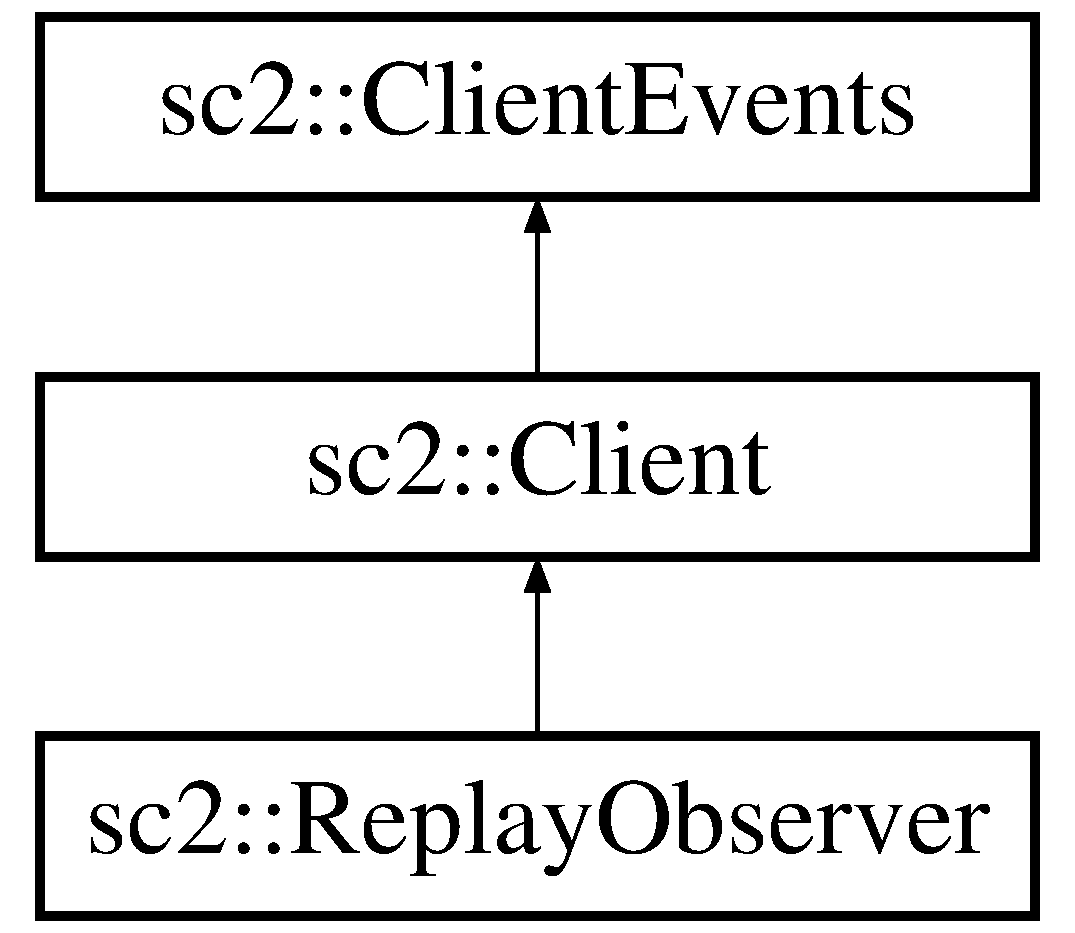
\includegraphics[height=3.000000cm]{classsc2_1_1_replay_observer}
\end{center}
\end{figure}
\subsection*{Public Member Functions}
\begin{DoxyCompactItemize}
\item 
\hyperlink{classsc2_1_1_replay_control_interface}{Replay\+Control\+Interface} $\ast$ \hyperlink{classsc2_1_1_replay_observer_a99198b2295dc998662b929f96ad17d65}{Replay\+Control} ()
\item 
virtual bool \hyperlink{classsc2_1_1_replay_observer_a35461e606619ea1f2c968e37ab164d5d}{Ignore\+Replay} (const \hyperlink{structsc2_1_1_replay_info}{Replay\+Info} \&replay\+\_\+info, uint32\+\_\+t \&player\+\_\+id)
\item 
\mbox{\Hypertarget{classsc2_1_1_replay_observer_ac0f3061d817e87afd8fd43753ffc3612}\label{classsc2_1_1_replay_observer_ac0f3061d817e87afd8fd43753ffc3612}} 
void {\bfseries Set\+Control} (\hyperlink{classsc2_1_1_control_interface}{Control\+Interface} $\ast$control)
\end{DoxyCompactItemize}


\subsection{Detailed Description}
A client for running a replay. 

\subsection{Member Function Documentation}
\mbox{\Hypertarget{classsc2_1_1_replay_observer_a35461e606619ea1f2c968e37ab164d5d}\label{classsc2_1_1_replay_observer_a35461e606619ea1f2c968e37ab164d5d}} 
\index{sc2\+::\+Replay\+Observer@{sc2\+::\+Replay\+Observer}!Ignore\+Replay@{Ignore\+Replay}}
\index{Ignore\+Replay@{Ignore\+Replay}!sc2\+::\+Replay\+Observer@{sc2\+::\+Replay\+Observer}}
\subsubsection{\texorpdfstring{Ignore\+Replay()}{IgnoreReplay()}}
{\footnotesize\ttfamily virtual bool sc2\+::\+Replay\+Observer\+::\+Ignore\+Replay (\begin{DoxyParamCaption}\item[{const \hyperlink{structsc2_1_1_replay_info}{Replay\+Info} \&}]{replay\+\_\+info,  }\item[{uint32\+\_\+t \&}]{player\+\_\+id }\end{DoxyParamCaption})\hspace{0.3cm}{\ttfamily [virtual]}}

Determines if the replay should be filtered out. 
\begin{DoxyParams}{Parameters}
{\em replay\+\_\+info} & Replay information used to decide if the replay should be filtered. \\
\hline
\end{DoxyParams}
\begin{DoxyReturn}{Returns}
If \textquotesingle{}true\textquotesingle{}, the replay will be rejected and not analyzed. 
\end{DoxyReturn}
\mbox{\Hypertarget{classsc2_1_1_replay_observer_a99198b2295dc998662b929f96ad17d65}\label{classsc2_1_1_replay_observer_a99198b2295dc998662b929f96ad17d65}} 
\index{sc2\+::\+Replay\+Observer@{sc2\+::\+Replay\+Observer}!Replay\+Control@{Replay\+Control}}
\index{Replay\+Control@{Replay\+Control}!sc2\+::\+Replay\+Observer@{sc2\+::\+Replay\+Observer}}
\subsubsection{\texorpdfstring{Replay\+Control()}{ReplayControl()}}
{\footnotesize\ttfamily \hyperlink{classsc2_1_1_replay_control_interface}{Replay\+Control\+Interface}$\ast$ sc2\+::\+Replay\+Observer\+::\+Replay\+Control (\begin{DoxyParamCaption}{ }\end{DoxyParamCaption})}

Obtains the replay control interface. \begin{DoxyReturn}{Returns}
The replay control interface. 
\end{DoxyReturn}


The documentation for this class was generated from the following file\+:\begin{DoxyCompactItemize}
\item 
include/sc2api/\hyperlink{sc2__replay__observer_8h}{sc2\+\_\+replay\+\_\+observer.\+h}\end{DoxyCompactItemize}

\hypertarget{structsc2_1_1_replay_player_info}{}\section{sc2\+:\+:Replay\+Player\+Info Struct Reference}
\label{structsc2_1_1_replay_player_info}\index{sc2\+::\+Replay\+Player\+Info@{sc2\+::\+Replay\+Player\+Info}}


Information about a player in a replay.  




{\ttfamily \#include $<$sc2\+\_\+gametypes.\+h$>$}

\subsection*{Public Attributes}
\begin{DoxyCompactItemize}
\item 
\mbox{\Hypertarget{structsc2_1_1_replay_player_info_a0a10ff4668dd1d3b017ff5d4da1837fc}\label{structsc2_1_1_replay_player_info_a0a10ff4668dd1d3b017ff5d4da1837fc}} 
int \hyperlink{structsc2_1_1_replay_player_info_a0a10ff4668dd1d3b017ff5d4da1837fc}{player\+\_\+id}
\begin{DoxyCompactList}\small\item\em Player ID. \end{DoxyCompactList}\item 
\mbox{\Hypertarget{structsc2_1_1_replay_player_info_a0a1d671f0ad7727dcb2c9b4b4a2b9314}\label{structsc2_1_1_replay_player_info_a0a1d671f0ad7727dcb2c9b4b4a2b9314}} 
int \hyperlink{structsc2_1_1_replay_player_info_a0a1d671f0ad7727dcb2c9b4b4a2b9314}{mmr}
\begin{DoxyCompactList}\small\item\em Player ranking. \end{DoxyCompactList}\item 
\mbox{\Hypertarget{structsc2_1_1_replay_player_info_aa9bd56433e96284ccf0b5107e03b1cf3}\label{structsc2_1_1_replay_player_info_aa9bd56433e96284ccf0b5107e03b1cf3}} 
int \hyperlink{structsc2_1_1_replay_player_info_aa9bd56433e96284ccf0b5107e03b1cf3}{apm}
\begin{DoxyCompactList}\small\item\em Player actions per minute. \end{DoxyCompactList}\item 
\mbox{\Hypertarget{structsc2_1_1_replay_player_info_a4ab3c2d0a8d9d784be2404c671f1d143}\label{structsc2_1_1_replay_player_info_a4ab3c2d0a8d9d784be2404c671f1d143}} 
Race \hyperlink{structsc2_1_1_replay_player_info_a4ab3c2d0a8d9d784be2404c671f1d143}{race}
\begin{DoxyCompactList}\small\item\em Actual player race. \end{DoxyCompactList}\item 
\mbox{\Hypertarget{structsc2_1_1_replay_player_info_ad8061fc9f5910207eff1faa2437cdfae}\label{structsc2_1_1_replay_player_info_ad8061fc9f5910207eff1faa2437cdfae}} 
Race \hyperlink{structsc2_1_1_replay_player_info_ad8061fc9f5910207eff1faa2437cdfae}{race\+\_\+selected}
\begin{DoxyCompactList}\small\item\em Selected player race. If the race is \char`\"{}\+Random\char`\"{}, the race data member may be different. \end{DoxyCompactList}\item 
\mbox{\Hypertarget{structsc2_1_1_replay_player_info_ad10393848e92ccfe4c2add12bd3528c5}\label{structsc2_1_1_replay_player_info_ad10393848e92ccfe4c2add12bd3528c5}} 
Game\+Result \hyperlink{structsc2_1_1_replay_player_info_ad10393848e92ccfe4c2add12bd3528c5}{game\+\_\+result}
\begin{DoxyCompactList}\small\item\em If the player won or lost. \end{DoxyCompactList}\end{DoxyCompactItemize}


\subsection{Detailed Description}
Information about a player in a replay. 

The documentation for this struct was generated from the following file\+:\begin{DoxyCompactItemize}
\item 
include/sc2api/\hyperlink{sc2__gametypes_8h}{sc2\+\_\+gametypes.\+h}\end{DoxyCompactItemize}

\hypertarget{structsc2_1_1_replay_settings}{}\section{sc2\+:\+:Replay\+Settings Struct Reference}
\label{structsc2_1_1_replay_settings}\index{sc2\+::\+Replay\+Settings@{sc2\+::\+Replay\+Settings}}


Settings for starting a replay.  




{\ttfamily \#include $<$sc2\+\_\+game\+\_\+settings.\+h$>$}

\subsection*{Public Attributes}
\begin{DoxyCompactItemize}
\item 
\mbox{\Hypertarget{structsc2_1_1_replay_settings_a918978a607ae7442102deb298e2063df}\label{structsc2_1_1_replay_settings_a918978a607ae7442102deb298e2063df}} 
std\+::vector$<$ std\+::string $>$ {\bfseries replay\+\_\+file}
\item 
\mbox{\Hypertarget{structsc2_1_1_replay_settings_af8a1ae47f40c2e026e7e56500bc09d6a}\label{structsc2_1_1_replay_settings_af8a1ae47f40c2e026e7e56500bc09d6a}} 
std\+::string {\bfseries replay\+\_\+dir}
\item 
\mbox{\Hypertarget{structsc2_1_1_replay_settings_a24e6faf9ea89fe0828421ad2af869ed7}\label{structsc2_1_1_replay_settings_a24e6faf9ea89fe0828421ad2af869ed7}} 
uint32\+\_\+t {\bfseries player\+\_\+id}
\end{DoxyCompactItemize}


\subsection{Detailed Description}
Settings for starting a replay. 

The documentation for this struct was generated from the following file\+:\begin{DoxyCompactItemize}
\item 
include/sc2api/sc2\+\_\+game\+\_\+settings.\+h\end{DoxyCompactItemize}

\hypertarget{classsc2_1_1_s_c2_type}{}\section{sc2\+:\+:S\+C2\+Type$<$ T $>$ Class Template Reference}
\label{classsc2_1_1_s_c2_type}\index{sc2\+::\+S\+C2\+Type$<$ T $>$@{sc2\+::\+S\+C2\+Type$<$ T $>$}}


{\ttfamily \#include $<$sc2\+\_\+types.\+h$>$}

\subsection*{Public Member Functions}
\begin{DoxyCompactItemize}
\item 
\mbox{\Hypertarget{classsc2_1_1_s_c2_type_a797ecedf348b295b1827f6cd875843e7}\label{classsc2_1_1_s_c2_type_a797ecedf348b295b1827f6cd875843e7}} 
\hyperlink{classsc2_1_1_s_c2_type_a797ecedf348b295b1827f6cd875843e7}{S\+C2\+Type} ()
\begin{DoxyCompactList}\small\item\em Default constructor. \end{DoxyCompactList}\item 
\mbox{\Hypertarget{classsc2_1_1_s_c2_type_adda8c2ecd47bf1fe93ad54726404674f}\label{classsc2_1_1_s_c2_type_adda8c2ecd47bf1fe93ad54726404674f}} 
\hyperlink{classsc2_1_1_s_c2_type_adda8c2ecd47bf1fe93ad54726404674f}{S\+C2\+Type} (uint32\+\_\+t type\+\_\+id)
\begin{DoxyCompactList}\small\item\em Construct from an integer, corresponds to the enum value. \end{DoxyCompactList}\item 
\mbox{\Hypertarget{classsc2_1_1_s_c2_type_ac956d32e3d7989b2e0ab2664c9822d16}\label{classsc2_1_1_s_c2_type_ac956d32e3d7989b2e0ab2664c9822d16}} 
\hyperlink{classsc2_1_1_s_c2_type_ac956d32e3d7989b2e0ab2664c9822d16}{S\+C2\+Type} (T type\+\_\+id)
\begin{DoxyCompactList}\small\item\em Construct from the enum. \end{DoxyCompactList}\item 
bool \hyperlink{classsc2_1_1_s_c2_type_a499b06e107c0561ce3d2d80094fbdd94}{operator==} (\hyperlink{classsc2_1_1_s_c2_type}{S\+C2\+Type}$<$ T $>$ type\+\_\+id) const
\item 
\mbox{\Hypertarget{classsc2_1_1_s_c2_type_a404a385de418d89ea84344d9ac7fd728}\label{classsc2_1_1_s_c2_type_a404a385de418d89ea84344d9ac7fd728}} 
bool {\bfseries operator==} (T type\+\_\+id) const
\item 
\mbox{\Hypertarget{classsc2_1_1_s_c2_type_a4dcadbfd52b9acde5f49b2d452ac08fa}\label{classsc2_1_1_s_c2_type_a4dcadbfd52b9acde5f49b2d452ac08fa}} 
bool {\bfseries operator==} (uint32\+\_\+t type\+\_\+id) const
\item 
\mbox{\Hypertarget{classsc2_1_1_s_c2_type_ade586b36531920f32527128774df00b7}\label{classsc2_1_1_s_c2_type_ade586b36531920f32527128774df00b7}} 
bool {\bfseries operator==} (int type\+\_\+id) const
\item 
bool \hyperlink{classsc2_1_1_s_c2_type_a6e032550a699843364b52d9f30d7ddcc}{operator!=} (\hyperlink{classsc2_1_1_s_c2_type}{S\+C2\+Type}$<$ T $>$ type\+\_\+id) const
\item 
\mbox{\Hypertarget{classsc2_1_1_s_c2_type_af18f2a54f07829ae2cc8501301f1764f}\label{classsc2_1_1_s_c2_type_af18f2a54f07829ae2cc8501301f1764f}} 
bool {\bfseries operator!=} (T type\+\_\+id) const
\item 
\mbox{\Hypertarget{classsc2_1_1_s_c2_type_afa64fdd5adf5eca49d3a95826e884fa1}\label{classsc2_1_1_s_c2_type_afa64fdd5adf5eca49d3a95826e884fa1}} 
bool {\bfseries operator!=} (uint32\+\_\+t type\+\_\+id) const
\item 
\mbox{\Hypertarget{classsc2_1_1_s_c2_type_a8195d6f42d7e7c193bf08dbd146ef22c}\label{classsc2_1_1_s_c2_type_a8195d6f42d7e7c193bf08dbd146ef22c}} 
bool {\bfseries operator!=} (int type\+\_\+id) const
\item 
\mbox{\Hypertarget{classsc2_1_1_s_c2_type_ab75e39605288070327604d10a5f720bf}\label{classsc2_1_1_s_c2_type_ab75e39605288070327604d10a5f720bf}} 
\hyperlink{classsc2_1_1_s_c2_type_ab75e39605288070327604d10a5f720bf}{operator uint32\+\_\+t} () const
\begin{DoxyCompactList}\small\item\em Cast to integer. \end{DoxyCompactList}\item 
\mbox{\Hypertarget{classsc2_1_1_s_c2_type_a16ef14791e484bcb2708d262fbfbc46f}\label{classsc2_1_1_s_c2_type_a16ef14791e484bcb2708d262fbfbc46f}} 
\hyperlink{classsc2_1_1_s_c2_type_a16ef14791e484bcb2708d262fbfbc46f}{operator T} () const
\begin{DoxyCompactList}\small\item\em Cast to enum type. \end{DoxyCompactList}\item 
bool \hyperlink{classsc2_1_1_s_c2_type_a359fd3f5911b611089dac072f2ba528f}{Is\+Valid} () const
\item 
std\+::string \hyperlink{classsc2_1_1_s_c2_type_a25533b72e301be4064d80a13c82dc506}{to\+\_\+string} () const
\item 
T \hyperlink{classsc2_1_1_s_c2_type_ada2d70972edaa615780f86165b7e87a3}{To\+Type} () const
\end{DoxyCompactItemize}


\subsection{Detailed Description}
\subsubsection*{template$<$class T$>$\newline
class sc2\+::\+S\+C2\+Type$<$ T $>$}

Template class for defining common game enum types. The template parameter is the enum. This class allows for seamless conversion between enum types and integers, while maintaining strong typing. This means, for example, that a unit type ID can be converted back and forth from an integer, but can\textquotesingle{}t be used when another type ID, e.\+g., an ability ID, is required as a parameter. 

\subsection{Member Function Documentation}
\mbox{\Hypertarget{classsc2_1_1_s_c2_type_a359fd3f5911b611089dac072f2ba528f}\label{classsc2_1_1_s_c2_type_a359fd3f5911b611089dac072f2ba528f}} 
\index{sc2\+::\+S\+C2\+Type@{sc2\+::\+S\+C2\+Type}!Is\+Valid@{Is\+Valid}}
\index{Is\+Valid@{Is\+Valid}!sc2\+::\+S\+C2\+Type@{sc2\+::\+S\+C2\+Type}}
\subsubsection{\texorpdfstring{Is\+Valid()}{IsValid()}}
{\footnotesize\ttfamily template$<$class T$>$ \\
bool \hyperlink{classsc2_1_1_s_c2_type}{sc2\+::\+S\+C2\+Type}$<$ T $>$\+::Is\+Valid (\begin{DoxyParamCaption}{ }\end{DoxyParamCaption}) const\hspace{0.3cm}{\ttfamily [inline]}}

Determines if the value contained is valid. \begin{DoxyReturn}{Returns}
\textquotesingle{}true\textquotesingle{} if the value is valid. 
\end{DoxyReturn}
\mbox{\Hypertarget{classsc2_1_1_s_c2_type_a6e032550a699843364b52d9f30d7ddcc}\label{classsc2_1_1_s_c2_type_a6e032550a699843364b52d9f30d7ddcc}} 
\index{sc2\+::\+S\+C2\+Type@{sc2\+::\+S\+C2\+Type}!operator"!=@{operator"!=}}
\index{operator"!=@{operator"!=}!sc2\+::\+S\+C2\+Type@{sc2\+::\+S\+C2\+Type}}
\subsubsection{\texorpdfstring{operator"!=()}{operator!=()}}
{\footnotesize\ttfamily template$<$class T$>$ \\
bool \hyperlink{classsc2_1_1_s_c2_type}{sc2\+::\+S\+C2\+Type}$<$ T $>$\+::operator!= (\begin{DoxyParamCaption}\item[{\hyperlink{classsc2_1_1_s_c2_type}{S\+C2\+Type}$<$ T $>$}]{type\+\_\+id }\end{DoxyParamCaption}) const\hspace{0.3cm}{\ttfamily [inline]}}

Test non-\/equivalence. \begin{DoxyReturn}{Returns}
\textquotesingle{}true\textquotesingle{} if the values are not equal. 
\end{DoxyReturn}
\mbox{\Hypertarget{classsc2_1_1_s_c2_type_a499b06e107c0561ce3d2d80094fbdd94}\label{classsc2_1_1_s_c2_type_a499b06e107c0561ce3d2d80094fbdd94}} 
\index{sc2\+::\+S\+C2\+Type@{sc2\+::\+S\+C2\+Type}!operator==@{operator==}}
\index{operator==@{operator==}!sc2\+::\+S\+C2\+Type@{sc2\+::\+S\+C2\+Type}}
\subsubsection{\texorpdfstring{operator==()}{operator==()}}
{\footnotesize\ttfamily template$<$class T$>$ \\
bool \hyperlink{classsc2_1_1_s_c2_type}{sc2\+::\+S\+C2\+Type}$<$ T $>$\+::operator== (\begin{DoxyParamCaption}\item[{\hyperlink{classsc2_1_1_s_c2_type}{S\+C2\+Type}$<$ T $>$}]{type\+\_\+id }\end{DoxyParamCaption}) const\hspace{0.3cm}{\ttfamily [inline]}}

Test equivalence. \begin{DoxyReturn}{Returns}
\textquotesingle{}true\textquotesingle{} if the values are equal. 
\end{DoxyReturn}
\mbox{\Hypertarget{classsc2_1_1_s_c2_type_a25533b72e301be4064d80a13c82dc506}\label{classsc2_1_1_s_c2_type_a25533b72e301be4064d80a13c82dc506}} 
\index{sc2\+::\+S\+C2\+Type@{sc2\+::\+S\+C2\+Type}!to\+\_\+string@{to\+\_\+string}}
\index{to\+\_\+string@{to\+\_\+string}!sc2\+::\+S\+C2\+Type@{sc2\+::\+S\+C2\+Type}}
\subsubsection{\texorpdfstring{to\+\_\+string()}{to\_string()}}
{\footnotesize\ttfamily template$<$class T$>$ \\
std\+::string \hyperlink{classsc2_1_1_s_c2_type}{sc2\+::\+S\+C2\+Type}$<$ T $>$\+::to\+\_\+string (\begin{DoxyParamCaption}{ }\end{DoxyParamCaption}) const\hspace{0.3cm}{\ttfamily [inline]}}

String of the integer value. \begin{DoxyReturn}{Returns}
The string of the value. 
\end{DoxyReturn}
\mbox{\Hypertarget{classsc2_1_1_s_c2_type_ada2d70972edaa615780f86165b7e87a3}\label{classsc2_1_1_s_c2_type_ada2d70972edaa615780f86165b7e87a3}} 
\index{sc2\+::\+S\+C2\+Type@{sc2\+::\+S\+C2\+Type}!To\+Type@{To\+Type}}
\index{To\+Type@{To\+Type}!sc2\+::\+S\+C2\+Type@{sc2\+::\+S\+C2\+Type}}
\subsubsection{\texorpdfstring{To\+Type()}{ToType()}}
{\footnotesize\ttfamily template$<$class T$>$ \\
T \hyperlink{classsc2_1_1_s_c2_type}{sc2\+::\+S\+C2\+Type}$<$ T $>$\+::To\+Type (\begin{DoxyParamCaption}{ }\end{DoxyParamCaption}) const\hspace{0.3cm}{\ttfamily [inline]}}

Explicit conversion to the enum type. \begin{DoxyReturn}{Returns}
The enum. 
\end{DoxyReturn}


The documentation for this class was generated from the following file\+:\begin{DoxyCompactItemize}
\item 
include/sc2api/\hyperlink{sc2__types_8h}{sc2\+\_\+types.\+h}\end{DoxyCompactItemize}

\hypertarget{structsc2_1_1_score}{}\section{sc2\+:\+:Score Struct Reference}
\label{structsc2_1_1_score}\index{sc2\+::\+Score@{sc2\+::\+Score}}


Scores.  




{\ttfamily \#include $<$sc2\+\_\+score.\+h$>$}

\subsection*{Public Member Functions}
\begin{DoxyCompactItemize}
\item 
\mbox{\Hypertarget{structsc2_1_1_score_a26f5b7adac31f862c6188f406ce7894a}\label{structsc2_1_1_score_a26f5b7adac31f862c6188f406ce7894a}} 
const float $\ast$ {\bfseries Raw\+Floats} () const
\item 
\mbox{\Hypertarget{structsc2_1_1_score_a673079c2e3409a261d4fb8f0041c33a9}\label{structsc2_1_1_score_a673079c2e3409a261d4fb8f0041c33a9}} 
bool {\bfseries Is\+Equal} (const \hyperlink{structsc2_1_1_score}{Score} \&other\+\_\+score) const
\end{DoxyCompactItemize}
\subsection*{Static Public Member Functions}
\begin{DoxyCompactItemize}
\item 
\mbox{\Hypertarget{structsc2_1_1_score_a3add288b1e757b796c3c9d8aea84549d}\label{structsc2_1_1_score_a3add288b1e757b796c3c9d8aea84549d}} 
static void {\bfseries Add\+Entries} (std\+::vector$<$ \hyperlink{structsc2_1_1_score_entry}{Score\+Entry} $>$ \&entries)
\end{DoxyCompactItemize}
\subsection*{Public Attributes}
\begin{DoxyCompactItemize}
\item 
\mbox{\Hypertarget{structsc2_1_1_score_a8c496fcfb02bec665857145af888f9a4}\label{structsc2_1_1_score_a8c496fcfb02bec665857145af888f9a4}} 
\hyperlink{sc2__score_8h_aa4e8dbe2d274f393f7afb290ba84657a}{Score\+Type} {\bfseries score\+\_\+type}
\item 
\mbox{\Hypertarget{structsc2_1_1_score_a3b442ae1a9aa764c01907d41b09d015f}\label{structsc2_1_1_score_a3b442ae1a9aa764c01907d41b09d015f}} 
float {\bfseries score}
\item 
\mbox{\Hypertarget{structsc2_1_1_score_a338f9ea8f1a55673d108375f8492e88e}\label{structsc2_1_1_score_a338f9ea8f1a55673d108375f8492e88e}} 
\hyperlink{structsc2_1_1_score_details}{Score\+Details} {\bfseries score\+\_\+details}
\end{DoxyCompactItemize}
\subsection*{Static Public Attributes}
\begin{DoxyCompactItemize}
\item 
\mbox{\Hypertarget{structsc2_1_1_score_aa4a528eb06bd12bb51ad73d98065adf2}\label{structsc2_1_1_score_aa4a528eb06bd12bb51ad73d98065adf2}} 
static const int {\bfseries float\+\_\+count\+\_\+} = sizeof(\hyperlink{structsc2_1_1_score_details}{Score\+Details}) / sizeof(float) + 1
\end{DoxyCompactItemize}


\subsection{Detailed Description}
Scores. 

The documentation for this struct was generated from the following file\+:\begin{DoxyCompactItemize}
\item 
include/sc2api/\hyperlink{sc2__score_8h}{sc2\+\_\+score.\+h}\end{DoxyCompactItemize}

\hypertarget{structsc2_1_1_score_details}{}\section{sc2\+:\+:Score\+Details Struct Reference}
\label{structsc2_1_1_score_details}\index{sc2\+::\+Score\+Details@{sc2\+::\+Score\+Details}}


Detailed scores.  




{\ttfamily \#include $<$sc2\+\_\+score.\+h$>$}

\subsection*{Static Public Member Functions}
\begin{DoxyCompactItemize}
\item 
\mbox{\Hypertarget{structsc2_1_1_score_details_ac0b693934fe7049b915c96149920a22b}\label{structsc2_1_1_score_details_ac0b693934fe7049b915c96149920a22b}} 
static void {\bfseries Add\+Entries} (\hyperlink{structsc2_1_1_score_entry}{Score\+Entry} base, std\+::vector$<$ \hyperlink{structsc2_1_1_score_entry}{Score\+Entry} $>$ \&entries)
\end{DoxyCompactItemize}
\subsection*{Public Attributes}
\begin{DoxyCompactItemize}
\item 
\mbox{\Hypertarget{structsc2_1_1_score_details_a3bf276c13fd180cc5f0507e767db9bf1}\label{structsc2_1_1_score_details_a3bf276c13fd180cc5f0507e767db9bf1}} 
float {\bfseries idle\+\_\+production\+\_\+time}
\item 
\mbox{\Hypertarget{structsc2_1_1_score_details_a774221683729e01a84793525b02c02b3}\label{structsc2_1_1_score_details_a774221683729e01a84793525b02c02b3}} 
float {\bfseries idle\+\_\+worker\+\_\+time}
\item 
\mbox{\Hypertarget{structsc2_1_1_score_details_a1fe5ed32bcfc749997d209b51feec46e}\label{structsc2_1_1_score_details_a1fe5ed32bcfc749997d209b51feec46e}} 
float {\bfseries total\+\_\+value\+\_\+units}
\item 
\mbox{\Hypertarget{structsc2_1_1_score_details_a7d083314efe5a5f807521342447dc75c}\label{structsc2_1_1_score_details_a7d083314efe5a5f807521342447dc75c}} 
float {\bfseries total\+\_\+value\+\_\+structures}
\item 
\mbox{\Hypertarget{structsc2_1_1_score_details_a568e358825efe99df79395e6919e6b11}\label{structsc2_1_1_score_details_a568e358825efe99df79395e6919e6b11}} 
float {\bfseries killed\+\_\+value\+\_\+units}
\item 
\mbox{\Hypertarget{structsc2_1_1_score_details_a48beb9fb69caa32831cbf64b5d9bcddc}\label{structsc2_1_1_score_details_a48beb9fb69caa32831cbf64b5d9bcddc}} 
float {\bfseries killed\+\_\+value\+\_\+structures}
\item 
\mbox{\Hypertarget{structsc2_1_1_score_details_aca2f06a073d92a1efa0f49dbb5cea3d9}\label{structsc2_1_1_score_details_aca2f06a073d92a1efa0f49dbb5cea3d9}} 
float {\bfseries collected\+\_\+minerals}
\item 
\mbox{\Hypertarget{structsc2_1_1_score_details_a665f82b64cdb0ceeecba5f4a8a21707c}\label{structsc2_1_1_score_details_a665f82b64cdb0ceeecba5f4a8a21707c}} 
float {\bfseries collected\+\_\+vespene}
\item 
\mbox{\Hypertarget{structsc2_1_1_score_details_a3623a9c630fc4a658aabfde4cf4a904f}\label{structsc2_1_1_score_details_a3623a9c630fc4a658aabfde4cf4a904f}} 
float {\bfseries collection\+\_\+rate\+\_\+minerals}
\item 
\mbox{\Hypertarget{structsc2_1_1_score_details_a5219f5e2cd1bb3ea672f68c9a4026b7f}\label{structsc2_1_1_score_details_a5219f5e2cd1bb3ea672f68c9a4026b7f}} 
float {\bfseries collection\+\_\+rate\+\_\+vespene}
\item 
\mbox{\Hypertarget{structsc2_1_1_score_details_a6db9dd6ab687a34aea62c6a1074e03f5}\label{structsc2_1_1_score_details_a6db9dd6ab687a34aea62c6a1074e03f5}} 
float {\bfseries spent\+\_\+minerals}
\item 
\mbox{\Hypertarget{structsc2_1_1_score_details_ad938d1101e98595d3c683d21d0ffbe6d}\label{structsc2_1_1_score_details_ad938d1101e98595d3c683d21d0ffbe6d}} 
float {\bfseries spent\+\_\+vespene}
\item 
\mbox{\Hypertarget{structsc2_1_1_score_details_a42a63e1818a43c70c3853dbdf99f316a}\label{structsc2_1_1_score_details_a42a63e1818a43c70c3853dbdf99f316a}} 
\hyperlink{structsc2_1_1_category_score_details}{Category\+Score\+Details} {\bfseries food\+\_\+used}
\item 
\mbox{\Hypertarget{structsc2_1_1_score_details_a180cb3239a939fd8d2e2f1c7e24bb6de}\label{structsc2_1_1_score_details_a180cb3239a939fd8d2e2f1c7e24bb6de}} 
\hyperlink{structsc2_1_1_category_score_details}{Category\+Score\+Details} {\bfseries killed\+\_\+minerals}
\item 
\mbox{\Hypertarget{structsc2_1_1_score_details_aff2476526af12a815f6f2a68205d4836}\label{structsc2_1_1_score_details_aff2476526af12a815f6f2a68205d4836}} 
\hyperlink{structsc2_1_1_category_score_details}{Category\+Score\+Details} {\bfseries killed\+\_\+vespene}
\item 
\mbox{\Hypertarget{structsc2_1_1_score_details_a9b9c2c4ef3a4981f165a44f237689157}\label{structsc2_1_1_score_details_a9b9c2c4ef3a4981f165a44f237689157}} 
\hyperlink{structsc2_1_1_category_score_details}{Category\+Score\+Details} {\bfseries lost\+\_\+minerals}
\item 
\mbox{\Hypertarget{structsc2_1_1_score_details_a27df2b050f1251205ebaa36a9e2dedd9}\label{structsc2_1_1_score_details_a27df2b050f1251205ebaa36a9e2dedd9}} 
\hyperlink{structsc2_1_1_category_score_details}{Category\+Score\+Details} {\bfseries lost\+\_\+vespene}
\item 
\mbox{\Hypertarget{structsc2_1_1_score_details_addf099d34243111cbb523bed0c356251}\label{structsc2_1_1_score_details_addf099d34243111cbb523bed0c356251}} 
\hyperlink{structsc2_1_1_category_score_details}{Category\+Score\+Details} {\bfseries friendly\+\_\+fire\+\_\+minerals}
\item 
\mbox{\Hypertarget{structsc2_1_1_score_details_af1bc2f8b18360147693558d58ec6671f}\label{structsc2_1_1_score_details_af1bc2f8b18360147693558d58ec6671f}} 
\hyperlink{structsc2_1_1_category_score_details}{Category\+Score\+Details} {\bfseries friendly\+\_\+fire\+\_\+vespene}
\item 
\mbox{\Hypertarget{structsc2_1_1_score_details_a6533ede42af915b467d858da1e69ec06}\label{structsc2_1_1_score_details_a6533ede42af915b467d858da1e69ec06}} 
\hyperlink{structsc2_1_1_category_score_details}{Category\+Score\+Details} {\bfseries used\+\_\+minerals}
\item 
\mbox{\Hypertarget{structsc2_1_1_score_details_aac4757a8c44d9b22dd7b570faab06496}\label{structsc2_1_1_score_details_aac4757a8c44d9b22dd7b570faab06496}} 
\hyperlink{structsc2_1_1_category_score_details}{Category\+Score\+Details} {\bfseries used\+\_\+vespene}
\item 
\mbox{\Hypertarget{structsc2_1_1_score_details_a5de20a8c62ae9ff6695064b435899150}\label{structsc2_1_1_score_details_a5de20a8c62ae9ff6695064b435899150}} 
\hyperlink{structsc2_1_1_category_score_details}{Category\+Score\+Details} {\bfseries total\+\_\+used\+\_\+minerals}
\item 
\mbox{\Hypertarget{structsc2_1_1_score_details_a95802d4b62fe1b42a86505e1677efbea}\label{structsc2_1_1_score_details_a95802d4b62fe1b42a86505e1677efbea}} 
\hyperlink{structsc2_1_1_category_score_details}{Category\+Score\+Details} {\bfseries total\+\_\+used\+\_\+vespene}
\item 
\mbox{\Hypertarget{structsc2_1_1_score_details_a159fcf0c814b80b20bee8b68a84e9d9e}\label{structsc2_1_1_score_details_a159fcf0c814b80b20bee8b68a84e9d9e}} 
\hyperlink{structsc2_1_1_vital_score_details}{Vital\+Score\+Details} {\bfseries total\+\_\+damage\+\_\+dealt}
\item 
\mbox{\Hypertarget{structsc2_1_1_score_details_a5ccd1a7da03561a74dde1f3c14182eac}\label{structsc2_1_1_score_details_a5ccd1a7da03561a74dde1f3c14182eac}} 
\hyperlink{structsc2_1_1_vital_score_details}{Vital\+Score\+Details} {\bfseries total\+\_\+damage\+\_\+taken}
\item 
\mbox{\Hypertarget{structsc2_1_1_score_details_af7303a1d1a9a3239f09efc1daccf57fd}\label{structsc2_1_1_score_details_af7303a1d1a9a3239f09efc1daccf57fd}} 
\hyperlink{structsc2_1_1_vital_score_details}{Vital\+Score\+Details} {\bfseries total\+\_\+healed}
\end{DoxyCompactItemize}


\subsection{Detailed Description}
Detailed scores. 

The documentation for this struct was generated from the following file\+:\begin{DoxyCompactItemize}
\item 
include/sc2api/\hyperlink{sc2__score_8h}{sc2\+\_\+score.\+h}\end{DoxyCompactItemize}

\hypertarget{structsc2_1_1_score_entry}{}\section{sc2\+:\+:Score\+Entry Struct Reference}
\label{structsc2_1_1_score_entry}\index{sc2\+::\+Score\+Entry@{sc2\+::\+Score\+Entry}}
\subsection*{Public Attributes}
\begin{DoxyCompactItemize}
\item 
\mbox{\Hypertarget{structsc2_1_1_score_entry_af7da48005cda508497512a3a67f2b603}\label{structsc2_1_1_score_entry_af7da48005cda508497512a3a67f2b603}} 
std\+::string {\bfseries name}
\item 
\mbox{\Hypertarget{structsc2_1_1_score_entry_a6d0b76b36b9e3cc8ec80b4271e8670ad}\label{structsc2_1_1_score_entry_a6d0b76b36b9e3cc8ec80b4271e8670ad}} 
int {\bfseries offset}
\item 
\mbox{\Hypertarget{structsc2_1_1_score_entry_a309550ccbfca6512390da1bc31e1cce9}\label{structsc2_1_1_score_entry_a309550ccbfca6512390da1bc31e1cce9}} 
bool {\bfseries use}
\item 
\mbox{\Hypertarget{structsc2_1_1_score_entry_afd936c62353a97b4fb04607e2a129293}\label{structsc2_1_1_score_entry_afd936c62353a97b4fb04607e2a129293}} 
bool {\bfseries nonzero}
\end{DoxyCompactItemize}


The documentation for this struct was generated from the following file\+:\begin{DoxyCompactItemize}
\item 
include/sc2api/\hyperlink{sc2__score_8h}{sc2\+\_\+score.\+h}\end{DoxyCompactItemize}

\hypertarget{structsc2_1_1_spatial_actions}{}\section{sc2\+:\+:Spatial\+Actions Struct Reference}
\label{structsc2_1_1_spatial_actions}\index{sc2\+::\+Spatial\+Actions@{sc2\+::\+Spatial\+Actions}}


Possible actions for feature layers.  




{\ttfamily \#include $<$sc2\+\_\+action.\+h$>$}

\subsection*{Public Attributes}
\begin{DoxyCompactItemize}
\item 
\mbox{\Hypertarget{structsc2_1_1_spatial_actions_a1ab964fd7e078894f25c7dddd881169c}\label{structsc2_1_1_spatial_actions_a1ab964fd7e078894f25c7dddd881169c}} 
std\+::vector$<$ \hyperlink{structsc2_1_1_spatial_unit_command}{Spatial\+Unit\+Command} $>$ \hyperlink{structsc2_1_1_spatial_actions_a1ab964fd7e078894f25c7dddd881169c}{unit\+\_\+commands}
\begin{DoxyCompactList}\small\item\em Commands to selected units. \end{DoxyCompactList}\item 
\mbox{\Hypertarget{structsc2_1_1_spatial_actions_aefbcb5de0d5ccb8871b73cf61682135d}\label{structsc2_1_1_spatial_actions_aefbcb5de0d5ccb8871b73cf61682135d}} 
std\+::vector$<$ \hyperlink{structsc2_1_1_spatial_camera_move}{Spatial\+Camera\+Move} $>$ \hyperlink{structsc2_1_1_spatial_actions_aefbcb5de0d5ccb8871b73cf61682135d}{camera\+\_\+moves}
\begin{DoxyCompactList}\small\item\em Camera movement. \end{DoxyCompactList}\item 
\mbox{\Hypertarget{structsc2_1_1_spatial_actions_ab836b6a65f6267552aa74d403aef7f0a}\label{structsc2_1_1_spatial_actions_ab836b6a65f6267552aa74d403aef7f0a}} 
std\+::vector$<$ \hyperlink{structsc2_1_1_spatial_select_point}{Spatial\+Select\+Point} $>$ \hyperlink{structsc2_1_1_spatial_actions_ab836b6a65f6267552aa74d403aef7f0a}{select\+\_\+points}
\begin{DoxyCompactList}\small\item\em Selecting by point. \end{DoxyCompactList}\item 
\mbox{\Hypertarget{structsc2_1_1_spatial_actions_abc60e7ad122ae7aec22d35f960c04d12}\label{structsc2_1_1_spatial_actions_abc60e7ad122ae7aec22d35f960c04d12}} 
std\+::vector$<$ \hyperlink{structsc2_1_1_spatial_select_rect}{Spatial\+Select\+Rect} $>$ \hyperlink{structsc2_1_1_spatial_actions_abc60e7ad122ae7aec22d35f960c04d12}{select\+\_\+rects}
\begin{DoxyCompactList}\small\item\em Selecting by rectangles. \end{DoxyCompactList}\end{DoxyCompactItemize}


\subsection{Detailed Description}
Possible actions for feature layers. 

The documentation for this struct was generated from the following file\+:\begin{DoxyCompactItemize}
\item 
include/sc2api/sc2\+\_\+action.\+h\end{DoxyCompactItemize}

\hypertarget{structsc2_1_1_spatial_camera_move}{}\section{sc2\+:\+:Spatial\+Camera\+Move Struct Reference}
\label{structsc2_1_1_spatial_camera_move}\index{sc2\+::\+Spatial\+Camera\+Move@{sc2\+::\+Spatial\+Camera\+Move}}


Where to move the camera to on the minimap.  




{\ttfamily \#include $<$sc2\+\_\+action.\+h$>$}

\subsection*{Public Attributes}
\begin{DoxyCompactItemize}
\item 
\mbox{\Hypertarget{structsc2_1_1_spatial_camera_move_a2b2187a5aeef5e3584eea5b7027bc659}\label{structsc2_1_1_spatial_camera_move_a2b2187a5aeef5e3584eea5b7027bc659}} 
\hyperlink{structsc2_1_1_point2_d_i}{Point2\+DI} {\bfseries center\+\_\+minimap}
\end{DoxyCompactItemize}


\subsection{Detailed Description}
Where to move the camera to on the minimap. 

The documentation for this struct was generated from the following file\+:\begin{DoxyCompactItemize}
\item 
include/sc2api/sc2\+\_\+action.\+h\end{DoxyCompactItemize}

\hypertarget{structsc2_1_1_spatial_select_point}{}\section{sc2\+:\+:Spatial\+Select\+Point Struct Reference}
\label{structsc2_1_1_spatial_select_point}\index{sc2\+::\+Spatial\+Select\+Point@{sc2\+::\+Spatial\+Select\+Point}}


Point selection.  




{\ttfamily \#include $<$sc2\+\_\+action.\+h$>$}

\subsection*{Public Attributes}
\begin{DoxyCompactItemize}
\item 
\mbox{\Hypertarget{structsc2_1_1_spatial_select_point_abbb6db879e35b38997c472619e7dc474}\label{structsc2_1_1_spatial_select_point_abbb6db879e35b38997c472619e7dc474}} 
\hyperlink{structsc2_1_1_point2_d_i}{Point2\+DI} {\bfseries select\+\_\+screen}
\item 
\mbox{\Hypertarget{structsc2_1_1_spatial_select_point_a393906b823f5fc96e72c8daebdc0e969}\label{structsc2_1_1_spatial_select_point_a393906b823f5fc96e72c8daebdc0e969}} 
Point\+Selection\+Type {\bfseries type}
\end{DoxyCompactItemize}


\subsection{Detailed Description}
Point selection. 

The documentation for this struct was generated from the following file\+:\begin{DoxyCompactItemize}
\item 
include/sc2api/sc2\+\_\+action.\+h\end{DoxyCompactItemize}

\hypertarget{structsc2_1_1_spatial_select_rect}{}\section{sc2\+:\+:Spatial\+Select\+Rect Struct Reference}
\label{structsc2_1_1_spatial_select_rect}\index{sc2\+::\+Spatial\+Select\+Rect@{sc2\+::\+Spatial\+Select\+Rect}}


{\ttfamily \#include $<$sc2\+\_\+action.\+h$>$}

\subsection*{Public Attributes}
\begin{DoxyCompactItemize}
\item 
\mbox{\Hypertarget{structsc2_1_1_spatial_select_rect_a4df6223c944de6e62d4577a2c8c86665}\label{structsc2_1_1_spatial_select_rect_a4df6223c944de6e62d4577a2c8c86665}} 
std\+::vector$<$ \hyperlink{structsc2_1_1_rect2_d_i}{Rect2\+DI} $>$ {\bfseries select\+\_\+screen}
\item 
\mbox{\Hypertarget{structsc2_1_1_spatial_select_rect_a761f039602b2de9ffa6a284983c815b5}\label{structsc2_1_1_spatial_select_rect_a761f039602b2de9ffa6a284983c815b5}} 
bool {\bfseries select\+\_\+add}
\end{DoxyCompactItemize}


\subsection{Detailed Description}
Rectangle selection. Equivalent to click-\/drag with the mouse. Multiple rectangles are allowed as the feature layer projection is orthogonal, and may not exactly work for the regular in-\/game perspective view. 

The documentation for this struct was generated from the following file\+:\begin{DoxyCompactItemize}
\item 
include/sc2api/sc2\+\_\+action.\+h\end{DoxyCompactItemize}

\hypertarget{structsc2_1_1_spatial_setup}{}\section{sc2\+:\+:Spatial\+Setup Struct Reference}
\label{structsc2_1_1_spatial_setup}\index{sc2\+::\+Spatial\+Setup@{sc2\+::\+Spatial\+Setup}}


Setup structure for feature layers or rendered images.  




{\ttfamily \#include $<$sc2\+\_\+map\+\_\+info.\+h$>$}

\subsection*{Public Attributes}
\begin{DoxyCompactItemize}
\item 
\mbox{\Hypertarget{structsc2_1_1_spatial_setup_a601930f7ac562ccfc63bda24e04cc384}\label{structsc2_1_1_spatial_setup_a601930f7ac562ccfc63bda24e04cc384}} 
float \hyperlink{structsc2_1_1_spatial_setup_a601930f7ac562ccfc63bda24e04cc384}{camera\+\_\+width}
\begin{DoxyCompactList}\small\item\em For feature layers only, determines the world space size of the camera. \end{DoxyCompactList}\item 
\mbox{\Hypertarget{structsc2_1_1_spatial_setup_a6b238b3ed5fd2d5d4f15dd096051d7ce}\label{structsc2_1_1_spatial_setup_a6b238b3ed5fd2d5d4f15dd096051d7ce}} 
int \hyperlink{structsc2_1_1_spatial_setup_a6b238b3ed5fd2d5d4f15dd096051d7ce}{map\+\_\+resolution\+\_\+x}
\begin{DoxyCompactList}\small\item\em Number of pixels in X of the main game view. \end{DoxyCompactList}\item 
\mbox{\Hypertarget{structsc2_1_1_spatial_setup_ae9e4415838b159f4a06a63af47fa148e}\label{structsc2_1_1_spatial_setup_ae9e4415838b159f4a06a63af47fa148e}} 
int \hyperlink{structsc2_1_1_spatial_setup_ae9e4415838b159f4a06a63af47fa148e}{map\+\_\+resolution\+\_\+y}
\begin{DoxyCompactList}\small\item\em Number of pixels in Y of the main game view. \end{DoxyCompactList}\item 
\mbox{\Hypertarget{structsc2_1_1_spatial_setup_aab77c57499ded735dfd268f710ae31b1}\label{structsc2_1_1_spatial_setup_aab77c57499ded735dfd268f710ae31b1}} 
int \hyperlink{structsc2_1_1_spatial_setup_aab77c57499ded735dfd268f710ae31b1}{minimap\+\_\+resolution\+\_\+x}
\begin{DoxyCompactList}\small\item\em Number of pixels in X of the minimap. \end{DoxyCompactList}\item 
\mbox{\Hypertarget{structsc2_1_1_spatial_setup_a930f3747e2f0a32e72220cd4a4ae90fd}\label{structsc2_1_1_spatial_setup_a930f3747e2f0a32e72220cd4a4ae90fd}} 
int \hyperlink{structsc2_1_1_spatial_setup_a930f3747e2f0a32e72220cd4a4ae90fd}{minimap\+\_\+resolution\+\_\+y}
\begin{DoxyCompactList}\small\item\em Number of pixels in Y of the minimap. \end{DoxyCompactList}\end{DoxyCompactItemize}


\subsection{Detailed Description}
Setup structure for feature layers or rendered images. 

The documentation for this struct was generated from the following file\+:\begin{DoxyCompactItemize}
\item 
include/sc2api/\hyperlink{sc2__map__info_8h}{sc2\+\_\+map\+\_\+info.\+h}\end{DoxyCompactItemize}

\hypertarget{structsc2_1_1_spatial_unit_command}{}\section{sc2\+:\+:Spatial\+Unit\+Command Struct Reference}
\label{structsc2_1_1_spatial_unit_command}\index{sc2\+::\+Spatial\+Unit\+Command@{sc2\+::\+Spatial\+Unit\+Command}}


An action (command or ability) applied to selected units when using feature layers or the rendered interface.  




{\ttfamily \#include $<$sc2\+\_\+action.\+h$>$}

\subsection*{Public Types}
\begin{DoxyCompactItemize}
\item 
enum \hyperlink{structsc2_1_1_spatial_unit_command_ad50a0bbdbaff9ef68fbda3d817d3a32e}{Target\+Type} \{ \hyperlink{structsc2_1_1_spatial_unit_command_ad50a0bbdbaff9ef68fbda3d817d3a32ea7f95fd3b8b1bbeb6221f223074dbbf9a}{Target\+Screen}, 
\hyperlink{structsc2_1_1_spatial_unit_command_ad50a0bbdbaff9ef68fbda3d817d3a32ea5c3cb6c9cf1642ef2579036167621b36}{Target\+Minimap}
 \}\begin{DoxyCompactList}\small\item\em If this action should apply to the screen or minimap. \end{DoxyCompactList}
\end{DoxyCompactItemize}
\subsection*{Public Attributes}
\begin{DoxyCompactItemize}
\item 
\mbox{\Hypertarget{structsc2_1_1_spatial_unit_command_a305cc8a0fe2a1364ddb853c8b9a5583c}\label{structsc2_1_1_spatial_unit_command_a305cc8a0fe2a1364ddb853c8b9a5583c}} 
\hyperlink{classsc2_1_1_s_c2_type}{Ability\+ID} \hyperlink{structsc2_1_1_spatial_unit_command_a305cc8a0fe2a1364ddb853c8b9a5583c}{ability\+\_\+id}
\begin{DoxyCompactList}\small\item\em The ID of the ability to invoke. \end{DoxyCompactList}\item 
\mbox{\Hypertarget{structsc2_1_1_spatial_unit_command_a48ea9dd08e0f49f2899ed2c69f9ade16}\label{structsc2_1_1_spatial_unit_command_a48ea9dd08e0f49f2899ed2c69f9ade16}} 
\hyperlink{structsc2_1_1_spatial_unit_command_ad50a0bbdbaff9ef68fbda3d817d3a32e}{Target\+Type} \hyperlink{structsc2_1_1_spatial_unit_command_a48ea9dd08e0f49f2899ed2c69f9ade16}{target\+\_\+type}
\begin{DoxyCompactList}\small\item\em If this action should be applied to the main game screen or the minimap. \end{DoxyCompactList}\item 
\mbox{\Hypertarget{structsc2_1_1_spatial_unit_command_aaf33b1b6790e5f5af4509a5c28ef1a9c}\label{structsc2_1_1_spatial_unit_command_aaf33b1b6790e5f5af4509a5c28ef1a9c}} 
\hyperlink{structsc2_1_1_point2_d_i}{Point2\+DI} \hyperlink{structsc2_1_1_spatial_unit_command_aaf33b1b6790e5f5af4509a5c28ef1a9c}{target}
\begin{DoxyCompactList}\small\item\em Target point on the screen or minimap, if required. \end{DoxyCompactList}\item 
\mbox{\Hypertarget{structsc2_1_1_spatial_unit_command_ae5cb8efec67b158fb1aaafd2491f38ea}\label{structsc2_1_1_spatial_unit_command_ae5cb8efec67b158fb1aaafd2491f38ea}} 
bool \hyperlink{structsc2_1_1_spatial_unit_command_ae5cb8efec67b158fb1aaafd2491f38ea}{queued}
\begin{DoxyCompactList}\small\item\em Indicates if this action should replace or queue behind other actions. \end{DoxyCompactList}\end{DoxyCompactItemize}


\subsection{Detailed Description}
An action (command or ability) applied to selected units when using feature layers or the rendered interface. 

\subsection{Member Enumeration Documentation}
\mbox{\Hypertarget{structsc2_1_1_spatial_unit_command_ad50a0bbdbaff9ef68fbda3d817d3a32e}\label{structsc2_1_1_spatial_unit_command_ad50a0bbdbaff9ef68fbda3d817d3a32e}} 
\index{sc2\+::\+Spatial\+Unit\+Command@{sc2\+::\+Spatial\+Unit\+Command}!Target\+Type@{Target\+Type}}
\index{Target\+Type@{Target\+Type}!sc2\+::\+Spatial\+Unit\+Command@{sc2\+::\+Spatial\+Unit\+Command}}
\subsubsection{\texorpdfstring{Target\+Type}{TargetType}}
{\footnotesize\ttfamily enum \hyperlink{structsc2_1_1_spatial_unit_command_ad50a0bbdbaff9ef68fbda3d817d3a32e}{sc2\+::\+Spatial\+Unit\+Command\+::\+Target\+Type}}



If this action should apply to the screen or minimap. 

\begin{DoxyEnumFields}{Enumerator}
\raisebox{\heightof{T}}[0pt][0pt]{\index{Target\+Screen@{Target\+Screen}!sc2\+::\+Spatial\+Unit\+Command@{sc2\+::\+Spatial\+Unit\+Command}}\index{sc2\+::\+Spatial\+Unit\+Command@{sc2\+::\+Spatial\+Unit\+Command}!Target\+Screen@{Target\+Screen}}}\mbox{\Hypertarget{structsc2_1_1_spatial_unit_command_ad50a0bbdbaff9ef68fbda3d817d3a32ea7f95fd3b8b1bbeb6221f223074dbbf9a}\label{structsc2_1_1_spatial_unit_command_ad50a0bbdbaff9ef68fbda3d817d3a32ea7f95fd3b8b1bbeb6221f223074dbbf9a}} 
Target\+Screen&Apply this action to the main game screen. \\
\hline

\raisebox{\heightof{T}}[0pt][0pt]{\index{Target\+Minimap@{Target\+Minimap}!sc2\+::\+Spatial\+Unit\+Command@{sc2\+::\+Spatial\+Unit\+Command}}\index{sc2\+::\+Spatial\+Unit\+Command@{sc2\+::\+Spatial\+Unit\+Command}!Target\+Minimap@{Target\+Minimap}}}\mbox{\Hypertarget{structsc2_1_1_spatial_unit_command_ad50a0bbdbaff9ef68fbda3d817d3a32ea5c3cb6c9cf1642ef2579036167621b36}\label{structsc2_1_1_spatial_unit_command_ad50a0bbdbaff9ef68fbda3d817d3a32ea5c3cb6c9cf1642ef2579036167621b36}} 
Target\+Minimap&Apply this action to the minimap. \\
\hline

\end{DoxyEnumFields}


The documentation for this struct was generated from the following file\+:\begin{DoxyCompactItemize}
\item 
include/sc2api/sc2\+\_\+action.\+h\end{DoxyCompactItemize}

\hypertarget{classsc2_1_1_unit}{}\section{sc2\+:\+:Unit Class Reference}
\label{classsc2_1_1_unit}\index{sc2\+::\+Unit@{sc2\+::\+Unit}}


A unit. Could be a structure, a worker or a military unit.  




{\ttfamily \#include $<$sc2\+\_\+unit.\+h$>$}

\subsection*{Public Types}
\begin{DoxyCompactItemize}
\item 
enum \hyperlink{classsc2_1_1_unit_af7815dad89107a05298c245b702ab270}{Display\+Type} \{ \hyperlink{classsc2_1_1_unit_af7815dad89107a05298c245b702ab270abd326f19234975ca23bb3265223d969d}{Visible} = 1, 
\hyperlink{classsc2_1_1_unit_af7815dad89107a05298c245b702ab270a0e970750301873d6ee4903e9bcb8d2c6}{Snapshot} = 2, 
\hyperlink{classsc2_1_1_unit_af7815dad89107a05298c245b702ab270a688e1743ab48c61d2e77ac6212f77cd9}{Hidden} = 3
 \}\begin{DoxyCompactList}\small\item\em If the unit is shown on screen or not. \end{DoxyCompactList}
\item 
enum \hyperlink{classsc2_1_1_unit_a5a40e672e7599d73ef8ef5758bbd7461}{Alliance} \{ \hyperlink{classsc2_1_1_unit_a5a40e672e7599d73ef8ef5758bbd7461af4dea1a00c973443e0d459bb522f7637}{Self} = 1, 
\hyperlink{classsc2_1_1_unit_a5a40e672e7599d73ef8ef5758bbd7461a2215843e5737efd34b268be16757ed27}{Ally} = 2, 
\hyperlink{classsc2_1_1_unit_a5a40e672e7599d73ef8ef5758bbd7461a50d778ca3f3c354474d27013b7eda3c1}{Neutral} = 3, 
\hyperlink{classsc2_1_1_unit_a5a40e672e7599d73ef8ef5758bbd7461a005610fbf80eaa3cc4ea28c26a42eae6}{Enemy} = 4
 \}\begin{DoxyCompactList}\small\item\em Relationship to this player. \end{DoxyCompactList}
\item 
enum \hyperlink{classsc2_1_1_unit_a03f99cfaa8ad4f9bba6cd0bc5586c943}{Cloak\+State} \{ \hyperlink{classsc2_1_1_unit_a03f99cfaa8ad4f9bba6cd0bc5586c943ac0cfb31c1521ab9e7759bfa12bf05b23}{Cloaked} = 1, 
\hyperlink{classsc2_1_1_unit_a03f99cfaa8ad4f9bba6cd0bc5586c943a4d1351a1f8046904bf4b089813b610b0}{Cloaked\+Detected} = 2, 
\hyperlink{classsc2_1_1_unit_a03f99cfaa8ad4f9bba6cd0bc5586c943a992a9de6738dc46b3ba64a6da9030f0f}{Not\+Cloaked} = 3, 
\hyperlink{classsc2_1_1_unit_a03f99cfaa8ad4f9bba6cd0bc5586c943a2cf1dac1fc0a53735ae998f1cd437446}{Unknown} = 4
 \}\begin{DoxyCompactList}\small\item\em \hyperlink{classsc2_1_1_unit}{Unit} cloak state. \end{DoxyCompactList}
\end{DoxyCompactItemize}
\subsection*{Public Member Functions}
\begin{DoxyCompactItemize}
\item 
\mbox{\Hypertarget{classsc2_1_1_unit_aca5722ffb5bc156d0e9d0b28a40fb7c1}\label{classsc2_1_1_unit_aca5722ffb5bc156d0e9d0b28a40fb7c1}} 
{\bfseries operator Tag} () const
\end{DoxyCompactItemize}
\subsection*{Public Attributes}
\begin{DoxyCompactItemize}
\item 
\mbox{\Hypertarget{classsc2_1_1_unit_a37330a1811b5fe37894d13d8b8f000ac}\label{classsc2_1_1_unit_a37330a1811b5fe37894d13d8b8f000ac}} 
\hyperlink{classsc2_1_1_unit_af7815dad89107a05298c245b702ab270}{Display\+Type} \hyperlink{classsc2_1_1_unit_a37330a1811b5fe37894d13d8b8f000ac}{display\+\_\+type}
\begin{DoxyCompactList}\small\item\em If the unit is shown on screen or not. \end{DoxyCompactList}\item 
\mbox{\Hypertarget{classsc2_1_1_unit_a639d0b3495e03ee28f5e91b16057d42b}\label{classsc2_1_1_unit_a639d0b3495e03ee28f5e91b16057d42b}} 
\hyperlink{classsc2_1_1_unit_a5a40e672e7599d73ef8ef5758bbd7461}{Alliance} \hyperlink{classsc2_1_1_unit_a639d0b3495e03ee28f5e91b16057d42b}{alliance}
\begin{DoxyCompactList}\small\item\em Relationship of the unit to this player. \end{DoxyCompactList}\item 
\mbox{\Hypertarget{classsc2_1_1_unit_a1312ee20e783753ee8ddf054878f7d9f}\label{classsc2_1_1_unit_a1312ee20e783753ee8ddf054878f7d9f}} 
Tag \hyperlink{classsc2_1_1_unit_a1312ee20e783753ee8ddf054878f7d9f}{tag}
\begin{DoxyCompactList}\small\item\em A unique identifier for the instance of a unit. \end{DoxyCompactList}\item 
\mbox{\Hypertarget{classsc2_1_1_unit_a4d7e26d2a7a33bc685fc3696dfed026f}\label{classsc2_1_1_unit_a4d7e26d2a7a33bc685fc3696dfed026f}} 
\hyperlink{classsc2_1_1_s_c2_type}{Unit\+Type\+ID} \hyperlink{classsc2_1_1_unit_a4d7e26d2a7a33bc685fc3696dfed026f}{unit\+\_\+type}
\begin{DoxyCompactList}\small\item\em An identifier of the type of unit. \end{DoxyCompactList}\item 
\mbox{\Hypertarget{classsc2_1_1_unit_a29fec2e9dff50d8504e8a2b32f7a1af0}\label{classsc2_1_1_unit_a29fec2e9dff50d8504e8a2b32f7a1af0}} 
int \hyperlink{classsc2_1_1_unit_a29fec2e9dff50d8504e8a2b32f7a1af0}{owner}
\begin{DoxyCompactList}\small\item\em Which player owns a unit. \end{DoxyCompactList}\item 
\mbox{\Hypertarget{classsc2_1_1_unit_adbe75d15c90712cb1e55e8b8bcbc1319}\label{classsc2_1_1_unit_adbe75d15c90712cb1e55e8b8bcbc1319}} 
\hyperlink{structsc2_1_1_point3_d}{Point3D} \hyperlink{classsc2_1_1_unit_adbe75d15c90712cb1e55e8b8bcbc1319}{pos}
\begin{DoxyCompactList}\small\item\em Position of the unit in the world. \end{DoxyCompactList}\item 
\mbox{\Hypertarget{classsc2_1_1_unit_a9f947f6dffd571c2ab89ddd53609a7f4}\label{classsc2_1_1_unit_a9f947f6dffd571c2ab89ddd53609a7f4}} 
float \hyperlink{classsc2_1_1_unit_a9f947f6dffd571c2ab89ddd53609a7f4}{facing}
\begin{DoxyCompactList}\small\item\em Direction the unit faces in radians (1 radian == 57.\+296 degrees) \end{DoxyCompactList}\item 
\mbox{\Hypertarget{classsc2_1_1_unit_a0c2d1fb9e6f150333d96cc8ce8f9e9bf}\label{classsc2_1_1_unit_a0c2d1fb9e6f150333d96cc8ce8f9e9bf}} 
float \hyperlink{classsc2_1_1_unit_a0c2d1fb9e6f150333d96cc8ce8f9e9bf}{radius}
\begin{DoxyCompactList}\small\item\em Radius of the unit. \end{DoxyCompactList}\item 
\mbox{\Hypertarget{classsc2_1_1_unit_abb3c46774c4d5dab4d641a4abcf68aba}\label{classsc2_1_1_unit_abb3c46774c4d5dab4d641a4abcf68aba}} 
float \hyperlink{classsc2_1_1_unit_abb3c46774c4d5dab4d641a4abcf68aba}{build\+\_\+progress}
\begin{DoxyCompactList}\small\item\em Gives progress under construction. Range\+: \mbox{[}0.\+0, 1.\+0\mbox{]}. 1.\+0 == finished. \end{DoxyCompactList}\item 
\mbox{\Hypertarget{classsc2_1_1_unit_ad06992e99ddf45f28be06550c61fabd4}\label{classsc2_1_1_unit_ad06992e99ddf45f28be06550c61fabd4}} 
\hyperlink{classsc2_1_1_unit_a03f99cfaa8ad4f9bba6cd0bc5586c943}{Cloak\+State} \hyperlink{classsc2_1_1_unit_ad06992e99ddf45f28be06550c61fabd4}{cloak}
\begin{DoxyCompactList}\small\item\em If the unit is cloaked. \end{DoxyCompactList}\item 
\mbox{\Hypertarget{classsc2_1_1_unit_a212a848d56f8ce323c1a8b5ac7bd0221}\label{classsc2_1_1_unit_a212a848d56f8ce323c1a8b5ac7bd0221}} 
float \hyperlink{classsc2_1_1_unit_a212a848d56f8ce323c1a8b5ac7bd0221}{detect\+\_\+range}
\begin{DoxyCompactList}\small\item\em Range of detector for detector units. \end{DoxyCompactList}\item 
\mbox{\Hypertarget{classsc2_1_1_unit_a22e99532761f81474b7e666e08bf8727}\label{classsc2_1_1_unit_a22e99532761f81474b7e666e08bf8727}} 
float \hyperlink{classsc2_1_1_unit_a22e99532761f81474b7e666e08bf8727}{radar\+\_\+range}
\begin{DoxyCompactList}\small\item\em Range of radar for units that are radar units. \end{DoxyCompactList}\item 
\mbox{\Hypertarget{classsc2_1_1_unit_afc532e894e9496c843ac00abce343f41}\label{classsc2_1_1_unit_afc532e894e9496c843ac00abce343f41}} 
bool \hyperlink{classsc2_1_1_unit_afc532e894e9496c843ac00abce343f41}{is\+\_\+selected}
\begin{DoxyCompactList}\small\item\em If the unit is in the current selection of the player. \end{DoxyCompactList}\item 
\mbox{\Hypertarget{classsc2_1_1_unit_a2766e02109100817ffd5135591746293}\label{classsc2_1_1_unit_a2766e02109100817ffd5135591746293}} 
bool \hyperlink{classsc2_1_1_unit_a2766e02109100817ffd5135591746293}{is\+\_\+on\+\_\+screen}
\begin{DoxyCompactList}\small\item\em Visible and within the camera frustum. \end{DoxyCompactList}\item 
\mbox{\Hypertarget{classsc2_1_1_unit_aa730ea2bf474d4422e6c6a1e267945d4}\label{classsc2_1_1_unit_aa730ea2bf474d4422e6c6a1e267945d4}} 
bool \hyperlink{classsc2_1_1_unit_aa730ea2bf474d4422e6c6a1e267945d4}{is\+\_\+blip}
\begin{DoxyCompactList}\small\item\em Detected by sensor tower. \end{DoxyCompactList}\item 
\mbox{\Hypertarget{classsc2_1_1_unit_a7049529d7ec06419b85121a384949abf}\label{classsc2_1_1_unit_a7049529d7ec06419b85121a384949abf}} 
float \hyperlink{classsc2_1_1_unit_a7049529d7ec06419b85121a384949abf}{health}
\begin{DoxyCompactList}\small\item\em Health of the unit. Not set for snapshots. \end{DoxyCompactList}\item 
\mbox{\Hypertarget{classsc2_1_1_unit_a9903ceca120d82cacc49dee00150fe67}\label{classsc2_1_1_unit_a9903ceca120d82cacc49dee00150fe67}} 
float \hyperlink{classsc2_1_1_unit_a9903ceca120d82cacc49dee00150fe67}{health\+\_\+max}
\begin{DoxyCompactList}\small\item\em Max health for the unit. Not set for snapshots. \end{DoxyCompactList}\item 
\mbox{\Hypertarget{classsc2_1_1_unit_ae5ee0c4d31a1266e31ac0a739bcc3d86}\label{classsc2_1_1_unit_ae5ee0c4d31a1266e31ac0a739bcc3d86}} 
float \hyperlink{classsc2_1_1_unit_ae5ee0c4d31a1266e31ac0a739bcc3d86}{shield}
\begin{DoxyCompactList}\small\item\em Shield of the unit. Not set for snapshots. \end{DoxyCompactList}\item 
\mbox{\Hypertarget{classsc2_1_1_unit_aa2b194b8a5499b7591356dc6365c0cdc}\label{classsc2_1_1_unit_aa2b194b8a5499b7591356dc6365c0cdc}} 
float \hyperlink{classsc2_1_1_unit_aa2b194b8a5499b7591356dc6365c0cdc}{energy}
\begin{DoxyCompactList}\small\item\em Energy of the unit. Not set for snapshots. \end{DoxyCompactList}\item 
\mbox{\Hypertarget{classsc2_1_1_unit_a689d7b7c9a68b3cd172f2333203423b9}\label{classsc2_1_1_unit_a689d7b7c9a68b3cd172f2333203423b9}} 
int \hyperlink{classsc2_1_1_unit_a689d7b7c9a68b3cd172f2333203423b9}{mineral\+\_\+contents}
\begin{DoxyCompactList}\small\item\em Amount of minerals if the unit is a mineral field. Not set for snapshots. \end{DoxyCompactList}\item 
\mbox{\Hypertarget{classsc2_1_1_unit_a76fcaa010a8a61b14b2839f49ef0f257}\label{classsc2_1_1_unit_a76fcaa010a8a61b14b2839f49ef0f257}} 
int \hyperlink{classsc2_1_1_unit_a76fcaa010a8a61b14b2839f49ef0f257}{vespene\+\_\+contents}
\begin{DoxyCompactList}\small\item\em Amount of vespene if the unit is a geyser. Not set for snapshots. \end{DoxyCompactList}\item 
\mbox{\Hypertarget{classsc2_1_1_unit_a6480f0b177f99a656ab3a273df3f8c3c}\label{classsc2_1_1_unit_a6480f0b177f99a656ab3a273df3f8c3c}} 
bool \hyperlink{classsc2_1_1_unit_a6480f0b177f99a656ab3a273df3f8c3c}{is\+\_\+flying}
\begin{DoxyCompactList}\small\item\em If the unit is flying. Not set for snapshots. \end{DoxyCompactList}\item 
\mbox{\Hypertarget{classsc2_1_1_unit_af815cd5269616209d4a2bdf2e734decb}\label{classsc2_1_1_unit_af815cd5269616209d4a2bdf2e734decb}} 
bool \hyperlink{classsc2_1_1_unit_af815cd5269616209d4a2bdf2e734decb}{is\+\_\+burrowed}
\begin{DoxyCompactList}\small\item\em If the unit is burrowed. Not set for snapshots. \end{DoxyCompactList}\item 
\mbox{\Hypertarget{classsc2_1_1_unit_a09bcc532a373b225b4ddb16fa77e9c41}\label{classsc2_1_1_unit_a09bcc532a373b225b4ddb16fa77e9c41}} 
float \hyperlink{classsc2_1_1_unit_a09bcc532a373b225b4ddb16fa77e9c41}{weapon\+\_\+cooldown}
\begin{DoxyCompactList}\small\item\em Time remaining for a weapon on cooldown. Not set for snapshots. \end{DoxyCompactList}\item 
\mbox{\Hypertarget{classsc2_1_1_unit_a45b97cf510454a385c372e512b40c51a}\label{classsc2_1_1_unit_a45b97cf510454a385c372e512b40c51a}} 
std\+::vector$<$ \hyperlink{structsc2_1_1_unit_order}{Unit\+Order} $>$ \hyperlink{classsc2_1_1_unit_a45b97cf510454a385c372e512b40c51a}{orders}
\begin{DoxyCompactList}\small\item\em Orders on a unit. Only valid for this player\textquotesingle{}s units. \end{DoxyCompactList}\item 
\mbox{\Hypertarget{classsc2_1_1_unit_a01b13cf74f1851983a834fdbf3e22b8a}\label{classsc2_1_1_unit_a01b13cf74f1851983a834fdbf3e22b8a}} 
Tag \hyperlink{classsc2_1_1_unit_a01b13cf74f1851983a834fdbf3e22b8a}{add\+\_\+on\+\_\+tag}
\begin{DoxyCompactList}\small\item\em Add-\/on like a tech lab or reactor. Only valid for this player\textquotesingle{}s units. \end{DoxyCompactList}\item 
\mbox{\Hypertarget{classsc2_1_1_unit_a01e2249c0d1bd27d8b61f233fbd75b66}\label{classsc2_1_1_unit_a01e2249c0d1bd27d8b61f233fbd75b66}} 
std\+::vector$<$ \hyperlink{structsc2_1_1_passenger_unit}{Passenger\+Unit} $>$ \hyperlink{classsc2_1_1_unit_a01e2249c0d1bd27d8b61f233fbd75b66}{passengers}
\begin{DoxyCompactList}\small\item\em Passengers in this transport. Only valid for this player\textquotesingle{}s units. \end{DoxyCompactList}\item 
\mbox{\Hypertarget{classsc2_1_1_unit_a59fb99084581bf4871a7de173931fc79}\label{classsc2_1_1_unit_a59fb99084581bf4871a7de173931fc79}} 
int \hyperlink{classsc2_1_1_unit_a59fb99084581bf4871a7de173931fc79}{cargo\+\_\+space\+\_\+taken}
\begin{DoxyCompactList}\small\item\em Number of cargo slots used in the transport. Only valid for this player\textquotesingle{}s units. \end{DoxyCompactList}\item 
\mbox{\Hypertarget{classsc2_1_1_unit_ab5dfd5b0c6f27a8a1f89b372260d9fb2}\label{classsc2_1_1_unit_ab5dfd5b0c6f27a8a1f89b372260d9fb2}} 
int \hyperlink{classsc2_1_1_unit_ab5dfd5b0c6f27a8a1f89b372260d9fb2}{cargo\+\_\+space\+\_\+max}
\begin{DoxyCompactList}\small\item\em Number of cargo slots available for a transport. Only valid for this player\textquotesingle{}s units. \end{DoxyCompactList}\item 
\mbox{\Hypertarget{classsc2_1_1_unit_aca42babe7fa2542782783a825fb99522}\label{classsc2_1_1_unit_aca42babe7fa2542782783a825fb99522}} 
int \hyperlink{classsc2_1_1_unit_aca42babe7fa2542782783a825fb99522}{assigned\+\_\+harvesters}
\begin{DoxyCompactList}\small\item\em Number of harvesters associated with a town hall (e.\+g., Command Center). Only valid for this player\textquotesingle{}s units. \end{DoxyCompactList}\item 
\mbox{\Hypertarget{classsc2_1_1_unit_a59c9e7c9c14f50f11d33b58716f664fe}\label{classsc2_1_1_unit_a59c9e7c9c14f50f11d33b58716f664fe}} 
int \hyperlink{classsc2_1_1_unit_a59c9e7c9c14f50f11d33b58716f664fe}{ideal\+\_\+harvesters}
\begin{DoxyCompactList}\small\item\em Number of harvesters that can be assigned to a town hall (e.\+g., Command Center). Only valid for this player\textquotesingle{}s units. \end{DoxyCompactList}\item 
\mbox{\Hypertarget{classsc2_1_1_unit_a0d1cc770a037ed2458bf944a787dcca5}\label{classsc2_1_1_unit_a0d1cc770a037ed2458bf944a787dcca5}} 
Tag \hyperlink{classsc2_1_1_unit_a0d1cc770a037ed2458bf944a787dcca5}{engaged\+\_\+target\+\_\+tag}
\begin{DoxyCompactList}\small\item\em Target unit of a unit. Only valid for this player\textquotesingle{}s units. \end{DoxyCompactList}\item 
\mbox{\Hypertarget{classsc2_1_1_unit_a34f17705c61114ad78c192ed7b06a9af}\label{classsc2_1_1_unit_a34f17705c61114ad78c192ed7b06a9af}} 
std\+::vector$<$ \hyperlink{classsc2_1_1_s_c2_type}{Buff\+ID} $>$ \hyperlink{classsc2_1_1_unit_a34f17705c61114ad78c192ed7b06a9af}{buffs}
\begin{DoxyCompactList}\small\item\em Buffs on this unit. Only valid for this player\textquotesingle{}s units. \end{DoxyCompactList}\end{DoxyCompactItemize}


\subsection{Detailed Description}
A unit. Could be a structure, a worker or a military unit. 

\subsection{Member Enumeration Documentation}
\mbox{\Hypertarget{classsc2_1_1_unit_a5a40e672e7599d73ef8ef5758bbd7461}\label{classsc2_1_1_unit_a5a40e672e7599d73ef8ef5758bbd7461}} 
\index{sc2\+::\+Unit@{sc2\+::\+Unit}!Alliance@{Alliance}}
\index{Alliance@{Alliance}!sc2\+::\+Unit@{sc2\+::\+Unit}}
\subsubsection{\texorpdfstring{Alliance}{Alliance}}
{\footnotesize\ttfamily enum \hyperlink{classsc2_1_1_unit_a5a40e672e7599d73ef8ef5758bbd7461}{sc2\+::\+Unit\+::\+Alliance}}



Relationship to this player. 

\begin{DoxyEnumFields}{Enumerator}
\raisebox{\heightof{T}}[0pt][0pt]{\index{Self@{Self}!sc2\+::\+Unit@{sc2\+::\+Unit}}\index{sc2\+::\+Unit@{sc2\+::\+Unit}!Self@{Self}}}\mbox{\Hypertarget{classsc2_1_1_unit_a5a40e672e7599d73ef8ef5758bbd7461af4dea1a00c973443e0d459bb522f7637}\label{classsc2_1_1_unit_a5a40e672e7599d73ef8ef5758bbd7461af4dea1a00c973443e0d459bb522f7637}} 
Self&Belongs to the player. \\
\hline

\raisebox{\heightof{T}}[0pt][0pt]{\index{Ally@{Ally}!sc2\+::\+Unit@{sc2\+::\+Unit}}\index{sc2\+::\+Unit@{sc2\+::\+Unit}!Ally@{Ally}}}\mbox{\Hypertarget{classsc2_1_1_unit_a5a40e672e7599d73ef8ef5758bbd7461a2215843e5737efd34b268be16757ed27}\label{classsc2_1_1_unit_a5a40e672e7599d73ef8ef5758bbd7461a2215843e5737efd34b268be16757ed27}} 
Ally&Ally of the player. \\
\hline

\raisebox{\heightof{T}}[0pt][0pt]{\index{Neutral@{Neutral}!sc2\+::\+Unit@{sc2\+::\+Unit}}\index{sc2\+::\+Unit@{sc2\+::\+Unit}!Neutral@{Neutral}}}\mbox{\Hypertarget{classsc2_1_1_unit_a5a40e672e7599d73ef8ef5758bbd7461a50d778ca3f3c354474d27013b7eda3c1}\label{classsc2_1_1_unit_a5a40e672e7599d73ef8ef5758bbd7461a50d778ca3f3c354474d27013b7eda3c1}} 
Neutral&A neutral unit, usually a non-\/player unit like a mineral field. \\
\hline

\raisebox{\heightof{T}}[0pt][0pt]{\index{Enemy@{Enemy}!sc2\+::\+Unit@{sc2\+::\+Unit}}\index{sc2\+::\+Unit@{sc2\+::\+Unit}!Enemy@{Enemy}}}\mbox{\Hypertarget{classsc2_1_1_unit_a5a40e672e7599d73ef8ef5758bbd7461a005610fbf80eaa3cc4ea28c26a42eae6}\label{classsc2_1_1_unit_a5a40e672e7599d73ef8ef5758bbd7461a005610fbf80eaa3cc4ea28c26a42eae6}} 
Enemy&Enemy of the player. \\
\hline

\end{DoxyEnumFields}
\mbox{\Hypertarget{classsc2_1_1_unit_a03f99cfaa8ad4f9bba6cd0bc5586c943}\label{classsc2_1_1_unit_a03f99cfaa8ad4f9bba6cd0bc5586c943}} 
\index{sc2\+::\+Unit@{sc2\+::\+Unit}!Cloak\+State@{Cloak\+State}}
\index{Cloak\+State@{Cloak\+State}!sc2\+::\+Unit@{sc2\+::\+Unit}}
\subsubsection{\texorpdfstring{Cloak\+State}{CloakState}}
{\footnotesize\ttfamily enum \hyperlink{classsc2_1_1_unit_a03f99cfaa8ad4f9bba6cd0bc5586c943}{sc2\+::\+Unit\+::\+Cloak\+State}}



\hyperlink{classsc2_1_1_unit}{Unit} cloak state. 

\begin{DoxyEnumFields}{Enumerator}
\raisebox{\heightof{T}}[0pt][0pt]{\index{Cloaked@{Cloaked}!sc2\+::\+Unit@{sc2\+::\+Unit}}\index{sc2\+::\+Unit@{sc2\+::\+Unit}!Cloaked@{Cloaked}}}\mbox{\Hypertarget{classsc2_1_1_unit_a03f99cfaa8ad4f9bba6cd0bc5586c943ac0cfb31c1521ab9e7759bfa12bf05b23}\label{classsc2_1_1_unit_a03f99cfaa8ad4f9bba6cd0bc5586c943ac0cfb31c1521ab9e7759bfa12bf05b23}} 
Cloaked&Cloaked, invisible to enemies until detected. \\
\hline

\raisebox{\heightof{T}}[0pt][0pt]{\index{Cloaked\+Detected@{Cloaked\+Detected}!sc2\+::\+Unit@{sc2\+::\+Unit}}\index{sc2\+::\+Unit@{sc2\+::\+Unit}!Cloaked\+Detected@{Cloaked\+Detected}}}\mbox{\Hypertarget{classsc2_1_1_unit_a03f99cfaa8ad4f9bba6cd0bc5586c943a4d1351a1f8046904bf4b089813b610b0}\label{classsc2_1_1_unit_a03f99cfaa8ad4f9bba6cd0bc5586c943a4d1351a1f8046904bf4b089813b610b0}} 
Cloaked\+Detected&Cloaked enemy, but detected. \\
\hline

\raisebox{\heightof{T}}[0pt][0pt]{\index{Not\+Cloaked@{Not\+Cloaked}!sc2\+::\+Unit@{sc2\+::\+Unit}}\index{sc2\+::\+Unit@{sc2\+::\+Unit}!Not\+Cloaked@{Not\+Cloaked}}}\mbox{\Hypertarget{classsc2_1_1_unit_a03f99cfaa8ad4f9bba6cd0bc5586c943a992a9de6738dc46b3ba64a6da9030f0f}\label{classsc2_1_1_unit_a03f99cfaa8ad4f9bba6cd0bc5586c943a992a9de6738dc46b3ba64a6da9030f0f}} 
Not\+Cloaked&No cloaking. \\
\hline

\raisebox{\heightof{T}}[0pt][0pt]{\index{Unknown@{Unknown}!sc2\+::\+Unit@{sc2\+::\+Unit}}\index{sc2\+::\+Unit@{sc2\+::\+Unit}!Unknown@{Unknown}}}\mbox{\Hypertarget{classsc2_1_1_unit_a03f99cfaa8ad4f9bba6cd0bc5586c943a2cf1dac1fc0a53735ae998f1cd437446}\label{classsc2_1_1_unit_a03f99cfaa8ad4f9bba6cd0bc5586c943a2cf1dac1fc0a53735ae998f1cd437446}} 
Unknown&Could not determine cloaking state. \\
\hline

\end{DoxyEnumFields}
\mbox{\Hypertarget{classsc2_1_1_unit_af7815dad89107a05298c245b702ab270}\label{classsc2_1_1_unit_af7815dad89107a05298c245b702ab270}} 
\index{sc2\+::\+Unit@{sc2\+::\+Unit}!Display\+Type@{Display\+Type}}
\index{Display\+Type@{Display\+Type}!sc2\+::\+Unit@{sc2\+::\+Unit}}
\subsubsection{\texorpdfstring{Display\+Type}{DisplayType}}
{\footnotesize\ttfamily enum \hyperlink{classsc2_1_1_unit_af7815dad89107a05298c245b702ab270}{sc2\+::\+Unit\+::\+Display\+Type}}



If the unit is shown on screen or not. 

\begin{DoxyEnumFields}{Enumerator}
\raisebox{\heightof{T}}[0pt][0pt]{\index{Visible@{Visible}!sc2\+::\+Unit@{sc2\+::\+Unit}}\index{sc2\+::\+Unit@{sc2\+::\+Unit}!Visible@{Visible}}}\mbox{\Hypertarget{classsc2_1_1_unit_af7815dad89107a05298c245b702ab270abd326f19234975ca23bb3265223d969d}\label{classsc2_1_1_unit_af7815dad89107a05298c245b702ab270abd326f19234975ca23bb3265223d969d}} 
Visible&\hyperlink{classsc2_1_1_unit}{Unit} will be visible. \\
\hline

\raisebox{\heightof{T}}[0pt][0pt]{\index{Snapshot@{Snapshot}!sc2\+::\+Unit@{sc2\+::\+Unit}}\index{sc2\+::\+Unit@{sc2\+::\+Unit}!Snapshot@{Snapshot}}}\mbox{\Hypertarget{classsc2_1_1_unit_af7815dad89107a05298c245b702ab270a0e970750301873d6ee4903e9bcb8d2c6}\label{classsc2_1_1_unit_af7815dad89107a05298c245b702ab270a0e970750301873d6ee4903e9bcb8d2c6}} 
Snapshot&\hyperlink{classsc2_1_1_unit}{Unit} is represented by a snapshot in the fog-\/of-\/war. This is for units that don\textquotesingle{}t belong to the player. The actual unit may be in a different location or state. \\
\hline

\raisebox{\heightof{T}}[0pt][0pt]{\index{Hidden@{Hidden}!sc2\+::\+Unit@{sc2\+::\+Unit}}\index{sc2\+::\+Unit@{sc2\+::\+Unit}!Hidden@{Hidden}}}\mbox{\Hypertarget{classsc2_1_1_unit_af7815dad89107a05298c245b702ab270a688e1743ab48c61d2e77ac6212f77cd9}\label{classsc2_1_1_unit_af7815dad89107a05298c245b702ab270a688e1743ab48c61d2e77ac6212f77cd9}} 
Hidden&\hyperlink{classsc2_1_1_unit}{Unit} will be hidden to enemies. \\
\hline

\end{DoxyEnumFields}


The documentation for this class was generated from the following file\+:\begin{DoxyCompactItemize}
\item 
include/sc2api/\hyperlink{sc2__unit_8h}{sc2\+\_\+unit.\+h}\end{DoxyCompactItemize}

\hypertarget{structsc2_1_1_unit_order}{}\section{sc2\+:\+:Unit\+Order Struct Reference}
\label{structsc2_1_1_unit_order}\index{sc2\+::\+Unit\+Order@{sc2\+::\+Unit\+Order}}


An order that is active on a unit.  




{\ttfamily \#include $<$sc2\+\_\+unit.\+h$>$}

\subsection*{Public Attributes}
\begin{DoxyCompactItemize}
\item 
\mbox{\Hypertarget{structsc2_1_1_unit_order_a0582df20b81543fd031972a497920d74}\label{structsc2_1_1_unit_order_a0582df20b81543fd031972a497920d74}} 
\hyperlink{classsc2_1_1_s_c2_type}{Ability\+ID} \hyperlink{structsc2_1_1_unit_order_a0582df20b81543fd031972a497920d74}{ability\+\_\+id}
\begin{DoxyCompactList}\small\item\em Ability ID that triggered the order. \end{DoxyCompactList}\item 
\mbox{\Hypertarget{structsc2_1_1_unit_order_aefffc0324bbb24f7dd7ab8def4e5afc2}\label{structsc2_1_1_unit_order_aefffc0324bbb24f7dd7ab8def4e5afc2}} 
Tag \hyperlink{structsc2_1_1_unit_order_aefffc0324bbb24f7dd7ab8def4e5afc2}{target\+\_\+unit\+\_\+tag}
\begin{DoxyCompactList}\small\item\em Target unit of the order, if there is one. \end{DoxyCompactList}\item 
\mbox{\Hypertarget{structsc2_1_1_unit_order_ae4c062864ad55c38faaf1e1abcb74671}\label{structsc2_1_1_unit_order_ae4c062864ad55c38faaf1e1abcb74671}} 
\hyperlink{structsc2_1_1_point2_d}{Point2D} \hyperlink{structsc2_1_1_unit_order_ae4c062864ad55c38faaf1e1abcb74671}{target\+\_\+pos}
\begin{DoxyCompactList}\small\item\em Target position of the order, if there is one. \end{DoxyCompactList}\item 
\mbox{\Hypertarget{structsc2_1_1_unit_order_a820bb8f79dcaebcd02475b5ac2c522cc}\label{structsc2_1_1_unit_order_a820bb8f79dcaebcd02475b5ac2c522cc}} 
float \hyperlink{structsc2_1_1_unit_order_a820bb8f79dcaebcd02475b5ac2c522cc}{progress}
\begin{DoxyCompactList}\small\item\em Progress of the order. \end{DoxyCompactList}\end{DoxyCompactItemize}


\subsection{Detailed Description}
An order that is active on a unit. 

The documentation for this struct was generated from the following file\+:\begin{DoxyCompactItemize}
\item 
include/sc2api/\hyperlink{sc2__unit_8h}{sc2\+\_\+unit.\+h}\end{DoxyCompactItemize}

\hypertarget{structsc2_1_1_unit_type_data}{}\section{sc2\+:\+:Unit\+Type\+Data Struct Reference}
\label{structsc2_1_1_unit_type_data}\index{sc2\+::\+Unit\+Type\+Data@{sc2\+::\+Unit\+Type\+Data}}


Data about a unit type. This data is derived from the catalog (xml) data of the game and upgrades.  




{\ttfamily \#include $<$sc2\+\_\+data.\+h$>$}

\subsection*{Public Member Functions}
\begin{DoxyCompactItemize}
\item 
\mbox{\Hypertarget{structsc2_1_1_unit_type_data_a69b29058353cf665ed27c32c1976f98b}\label{structsc2_1_1_unit_type_data_a69b29058353cf665ed27c32c1976f98b}} 
\hyperlink{structsc2_1_1_unit_type_data_a69b29058353cf665ed27c32c1976f98b}{Unit\+Type\+Data} ()
\begin{DoxyCompactList}\small\item\em Constructor. \end{DoxyCompactList}\item 
void \hyperlink{structsc2_1_1_unit_type_data_a4d05b07420d5c202b9f397968428254d}{Read\+From\+Proto} (const S\+C2\+A\+P\+I\+Protocol\+::\+Unit\+Type\+Data \&unit\+\_\+data)
\item 
\mbox{\Hypertarget{structsc2_1_1_unit_type_data_a815413cf7f47aa41f20c3399b7d6f58c}\label{structsc2_1_1_unit_type_data_a815413cf7f47aa41f20c3399b7d6f58c}} 
std\+::string \hyperlink{structsc2_1_1_unit_type_data_a815413cf7f47aa41f20c3399b7d6f58c}{Log} () const
\begin{DoxyCompactList}\small\item\em Serialize this unit type to a string. \end{DoxyCompactList}\end{DoxyCompactItemize}
\subsection*{Public Attributes}
\begin{DoxyCompactItemize}
\item 
\mbox{\Hypertarget{structsc2_1_1_unit_type_data_a43563832b7287316ce6d1ff909dda831}\label{structsc2_1_1_unit_type_data_a43563832b7287316ce6d1ff909dda831}} 
\hyperlink{classsc2_1_1_s_c2_type}{Unit\+Type\+ID} \hyperlink{structsc2_1_1_unit_type_data_a43563832b7287316ce6d1ff909dda831}{unit\+\_\+type\+\_\+id}
\begin{DoxyCompactList}\small\item\em Stable ID. This ID will not change between patches. \end{DoxyCompactList}\item 
\mbox{\Hypertarget{structsc2_1_1_unit_type_data_aefb802f470411fdba19e6b4ecb503427}\label{structsc2_1_1_unit_type_data_aefb802f470411fdba19e6b4ecb503427}} 
std\+::string \hyperlink{structsc2_1_1_unit_type_data_aefb802f470411fdba19e6b4ecb503427}{name}
\begin{DoxyCompactList}\small\item\em \hyperlink{classsc2_1_1_unit}{Unit} type name, corresponds to the game\textquotesingle{}s catalog. \end{DoxyCompactList}\item 
\mbox{\Hypertarget{structsc2_1_1_unit_type_data_a9269cf7ef9d4907c467b5367e5a6f210}\label{structsc2_1_1_unit_type_data_a9269cf7ef9d4907c467b5367e5a6f210}} 
bool \hyperlink{structsc2_1_1_unit_type_data_a9269cf7ef9d4907c467b5367e5a6f210}{available}
\begin{DoxyCompactList}\small\item\em If true, the unit is available to the current mods/map. \end{DoxyCompactList}\item 
\mbox{\Hypertarget{structsc2_1_1_unit_type_data_a13ab317cd91246aa40c928f48b801b38}\label{structsc2_1_1_unit_type_data_a13ab317cd91246aa40c928f48b801b38}} 
uint32\+\_\+t \hyperlink{structsc2_1_1_unit_type_data_a13ab317cd91246aa40c928f48b801b38}{cargo\+\_\+size}
\begin{DoxyCompactList}\small\item\em Number of cargo slots they occupy in a transport. \end{DoxyCompactList}\item 
\mbox{\Hypertarget{structsc2_1_1_unit_type_data_a50b767a68415cb1acbf246ee7f52ddcb}\label{structsc2_1_1_unit_type_data_a50b767a68415cb1acbf246ee7f52ddcb}} 
int \hyperlink{structsc2_1_1_unit_type_data_a50b767a68415cb1acbf246ee7f52ddcb}{mineral\+\_\+cost}
\begin{DoxyCompactList}\small\item\em Cost in minerals to build this unit type. \end{DoxyCompactList}\item 
\mbox{\Hypertarget{structsc2_1_1_unit_type_data_af596e50795f2b903b633cc7a72d43ae5}\label{structsc2_1_1_unit_type_data_af596e50795f2b903b633cc7a72d43ae5}} 
int \hyperlink{structsc2_1_1_unit_type_data_af596e50795f2b903b633cc7a72d43ae5}{vespene\+\_\+cost}
\begin{DoxyCompactList}\small\item\em Cost in vespene to build this unit type. \end{DoxyCompactList}\item 
\mbox{\Hypertarget{structsc2_1_1_unit_type_data_a1a07aba0d860ed9439104895ef2fc1f9}\label{structsc2_1_1_unit_type_data_a1a07aba0d860ed9439104895ef2fc1f9}} 
std\+::vector$<$ Attribute $>$ \hyperlink{structsc2_1_1_unit_type_data_a1a07aba0d860ed9439104895ef2fc1f9}{attributes}
\begin{DoxyCompactList}\small\item\em \hyperlink{classsc2_1_1_unit}{Unit} attributes, may change based on upgrades. \end{DoxyCompactList}\item 
\mbox{\Hypertarget{structsc2_1_1_unit_type_data_ac26ad858a8101e13d323c4111df9700b}\label{structsc2_1_1_unit_type_data_ac26ad858a8101e13d323c4111df9700b}} 
float \hyperlink{structsc2_1_1_unit_type_data_ac26ad858a8101e13d323c4111df9700b}{movement\+\_\+speed}
\begin{DoxyCompactList}\small\item\em Movement speed of unit type. \end{DoxyCompactList}\item 
\mbox{\Hypertarget{structsc2_1_1_unit_type_data_afadeb2efc945bac24492cd4efd0dba28}\label{structsc2_1_1_unit_type_data_afadeb2efc945bac24492cd4efd0dba28}} 
float \hyperlink{structsc2_1_1_unit_type_data_afadeb2efc945bac24492cd4efd0dba28}{armor}
\begin{DoxyCompactList}\small\item\em Armor of unit type. \end{DoxyCompactList}\item 
\mbox{\Hypertarget{structsc2_1_1_unit_type_data_aad375db4df763eafc47589a1b20c8553}\label{structsc2_1_1_unit_type_data_aad375db4df763eafc47589a1b20c8553}} 
std\+::vector$<$ \hyperlink{structsc2_1_1_weapon}{Weapon} $>$ \hyperlink{structsc2_1_1_unit_type_data_aad375db4df763eafc47589a1b20c8553}{weapons}
\begin{DoxyCompactList}\small\item\em Weapons on this unit type. \end{DoxyCompactList}\end{DoxyCompactItemize}


\subsection{Detailed Description}
Data about a unit type. This data is derived from the catalog (xml) data of the game and upgrades. 

\subsection{Member Function Documentation}
\mbox{\Hypertarget{structsc2_1_1_unit_type_data_a4d05b07420d5c202b9f397968428254d}\label{structsc2_1_1_unit_type_data_a4d05b07420d5c202b9f397968428254d}} 
\index{sc2\+::\+Unit\+Type\+Data@{sc2\+::\+Unit\+Type\+Data}!Read\+From\+Proto@{Read\+From\+Proto}}
\index{Read\+From\+Proto@{Read\+From\+Proto}!sc2\+::\+Unit\+Type\+Data@{sc2\+::\+Unit\+Type\+Data}}
\subsubsection{\texorpdfstring{Read\+From\+Proto()}{ReadFromProto()}}
{\footnotesize\ttfamily void sc2\+::\+Unit\+Type\+Data\+::\+Read\+From\+Proto (\begin{DoxyParamCaption}\item[{const S\+C2\+A\+P\+I\+Protocol\+::\+Unit\+Type\+Data \&}]{unit\+\_\+data }\end{DoxyParamCaption})}

Serialize this ability entry from the .proto file (used internally). 
\begin{DoxyParams}{Parameters}
{\em unit\+\_\+data} & The proto entry for this ability. \\
\hline
\end{DoxyParams}


The documentation for this struct was generated from the following file\+:\begin{DoxyCompactItemize}
\item 
include/sc2api/sc2\+\_\+data.\+h\end{DoxyCompactItemize}

\hypertarget{structsc2_1_1_upgrade_data}{}\section{sc2\+:\+:Upgrade\+Data Struct Reference}
\label{structsc2_1_1_upgrade_data}\index{sc2\+::\+Upgrade\+Data@{sc2\+::\+Upgrade\+Data}}


Upgrade data.  




{\ttfamily \#include $<$sc2\+\_\+data.\+h$>$}

\subsection*{Public Member Functions}
\begin{DoxyCompactItemize}
\item 
\mbox{\Hypertarget{structsc2_1_1_upgrade_data_a14c5db44ff8de245a4cd01592c3e6eeb}\label{structsc2_1_1_upgrade_data_a14c5db44ff8de245a4cd01592c3e6eeb}} 
void {\bfseries Read\+From\+Proto} (const S\+C2\+A\+P\+I\+Protocol\+::\+Upgrade\+Data \&upgrade\+\_\+data)
\item 
\mbox{\Hypertarget{structsc2_1_1_upgrade_data_ab9641667d3a1ba0bb61ebd892a3fa8a5}\label{structsc2_1_1_upgrade_data_ab9641667d3a1ba0bb61ebd892a3fa8a5}} 
std\+::string {\bfseries Log} () const
\end{DoxyCompactItemize}
\subsection*{Public Attributes}
\begin{DoxyCompactItemize}
\item 
\mbox{\Hypertarget{structsc2_1_1_upgrade_data_a029e671b0ca85d874b3723cae5f9b9ef}\label{structsc2_1_1_upgrade_data_a029e671b0ca85d874b3723cae5f9b9ef}} 
uint32\+\_\+t {\bfseries upgrade\+\_\+id}
\item 
\mbox{\Hypertarget{structsc2_1_1_upgrade_data_a8d8a126e4bee8c434bad896d3ac2c9be}\label{structsc2_1_1_upgrade_data_a8d8a126e4bee8c434bad896d3ac2c9be}} 
std\+::string {\bfseries name}
\end{DoxyCompactItemize}


\subsection{Detailed Description}
Upgrade data. 

The documentation for this struct was generated from the following file\+:\begin{DoxyCompactItemize}
\item 
include/sc2api/sc2\+\_\+data.\+h\end{DoxyCompactItemize}

\hypertarget{structsc2_1_1_vital_score_details}{}\section{sc2\+:\+:Vital\+Score\+Details Struct Reference}
\label{structsc2_1_1_vital_score_details}\index{sc2\+::\+Vital\+Score\+Details@{sc2\+::\+Vital\+Score\+Details}}


\hyperlink{structsc2_1_1_score}{Score} for vitals.  




{\ttfamily \#include $<$sc2\+\_\+score.\+h$>$}

\subsection*{Static Public Member Functions}
\begin{DoxyCompactItemize}
\item 
\mbox{\Hypertarget{structsc2_1_1_vital_score_details_adfe7fda209f61db978d18a5a70d4b75b}\label{structsc2_1_1_vital_score_details_adfe7fda209f61db978d18a5a70d4b75b}} 
static void {\bfseries Add\+Entries} (\hyperlink{structsc2_1_1_score_entry}{Score\+Entry} base, std\+::vector$<$ \hyperlink{structsc2_1_1_score_entry}{Score\+Entry} $>$ \&entries)
\end{DoxyCompactItemize}
\subsection*{Public Attributes}
\begin{DoxyCompactItemize}
\item 
\mbox{\Hypertarget{structsc2_1_1_vital_score_details_a9e2038167b6e5297c9f50da7cfd4192c}\label{structsc2_1_1_vital_score_details_a9e2038167b6e5297c9f50da7cfd4192c}} 
float {\bfseries life}
\item 
\mbox{\Hypertarget{structsc2_1_1_vital_score_details_a9473036d04928663c38f6c485b75b619}\label{structsc2_1_1_vital_score_details_a9473036d04928663c38f6c485b75b619}} 
float {\bfseries shields}
\item 
\mbox{\Hypertarget{structsc2_1_1_vital_score_details_a896de7149c5e4b19d81700e633140bca}\label{structsc2_1_1_vital_score_details_a896de7149c5e4b19d81700e633140bca}} 
float {\bfseries energy}
\end{DoxyCompactItemize}


\subsection{Detailed Description}
\hyperlink{structsc2_1_1_score}{Score} for vitals. 

The documentation for this struct was generated from the following file\+:\begin{DoxyCompactItemize}
\item 
include/sc2api/\hyperlink{sc2__score_8h}{sc2\+\_\+score.\+h}\end{DoxyCompactItemize}

\hypertarget{structsc2_1_1_weapon}{}\section{sc2\+:\+:Weapon Struct Reference}
\label{structsc2_1_1_weapon}\index{sc2\+::\+Weapon@{sc2\+::\+Weapon}}


\hyperlink{classsc2_1_1_unit}{Unit} weapon.  




{\ttfamily \#include $<$sc2\+\_\+data.\+h$>$}

\subsection*{Public Types}
\begin{DoxyCompactItemize}
\item 
\mbox{\Hypertarget{structsc2_1_1_weapon_a5ac5271d54e35bca7116578a00d86276}\label{structsc2_1_1_weapon_a5ac5271d54e35bca7116578a00d86276}} 
enum {\bfseries Target\+Type} \{ {\bfseries Ground} = 1, 
{\bfseries Air} = 2, 
{\bfseries Any} = 3, 
{\bfseries Invalid} = 4
 \}
\end{DoxyCompactItemize}
\subsection*{Public Member Functions}
\begin{DoxyCompactItemize}
\item 
\mbox{\Hypertarget{structsc2_1_1_weapon_a7489faf0444c6b3110d7609065242dc4}\label{structsc2_1_1_weapon_a7489faf0444c6b3110d7609065242dc4}} 
void {\bfseries Read\+From\+Proto} (const S\+C2\+A\+P\+I\+Protocol\+::\+Weapon \&weapon)
\end{DoxyCompactItemize}
\subsection*{Public Attributes}
\begin{DoxyCompactItemize}
\item 
\mbox{\Hypertarget{structsc2_1_1_weapon_a01a16b93a7ebf597ab92819f1983058f}\label{structsc2_1_1_weapon_a01a16b93a7ebf597ab92819f1983058f}} 
Target\+Type {\bfseries type}
\item 
\mbox{\Hypertarget{structsc2_1_1_weapon_ae0eb020a8b5df534b5921445a5148a7e}\label{structsc2_1_1_weapon_ae0eb020a8b5df534b5921445a5148a7e}} 
float {\bfseries damage\+\_\+}
\item 
\mbox{\Hypertarget{structsc2_1_1_weapon_a2c6805c104afc8e5f7351fadfed662c7}\label{structsc2_1_1_weapon_a2c6805c104afc8e5f7351fadfed662c7}} 
std\+::vector$<$ \hyperlink{structsc2_1_1_damage_bonus}{Damage\+Bonus} $>$ {\bfseries damage\+\_\+bonus}
\item 
\mbox{\Hypertarget{structsc2_1_1_weapon_a94f96140ceda50d81831f25880ecb53d}\label{structsc2_1_1_weapon_a94f96140ceda50d81831f25880ecb53d}} 
uint32\+\_\+t {\bfseries attacks}
\item 
\mbox{\Hypertarget{structsc2_1_1_weapon_a2e1f8b010cb5f427893e0441ba04e557}\label{structsc2_1_1_weapon_a2e1f8b010cb5f427893e0441ba04e557}} 
float {\bfseries range}
\item 
\mbox{\Hypertarget{structsc2_1_1_weapon_a36a66499bcad3c59386f861fb439bab0}\label{structsc2_1_1_weapon_a36a66499bcad3c59386f861fb439bab0}} 
float {\bfseries speed}
\end{DoxyCompactItemize}


\subsection{Detailed Description}
\hyperlink{classsc2_1_1_unit}{Unit} weapon. 

The documentation for this struct was generated from the following file\+:\begin{DoxyCompactItemize}
\item 
include/sc2api/sc2\+\_\+data.\+h\end{DoxyCompactItemize}

\chapter{File Documentation}
\hypertarget{sc2__client_8h}{}\section{include/sc2api/sc2\+\_\+client.h File Reference}
\label{sc2__client_8h}\index{include/sc2api/sc2\+\_\+client.\+h@{include/sc2api/sc2\+\_\+client.\+h}}


The base class for Agent and Replay\+Observer.  


{\ttfamily \#include $<$string$>$}\newline
{\ttfamily \#include $<$vector$>$}\newline
{\ttfamily \#include $<$cassert$>$}\newline
{\ttfamily \#include \char`\"{}sc2api/sc2\+\_\+typeenums.\+h\char`\"{}}\newline
\subsection*{Classes}
\begin{DoxyCompactItemize}
\item 
class \hyperlink{classsc2_1_1_client_events}{sc2\+::\+Client\+Events}
\begin{DoxyCompactList}\small\item\em A set of common events a user can override in their derived bot or replay observer class. \end{DoxyCompactList}\item 
class \hyperlink{classsc2_1_1_client}{sc2\+::\+Client}
\begin{DoxyCompactList}\small\item\em The base class for \hyperlink{classsc2_1_1_agent}{Agent} and \hyperlink{classsc2_1_1_replay_observer}{Replay\+Observer}. \end{DoxyCompactList}\end{DoxyCompactItemize}
\subsection*{Enumerations}
\begin{DoxyCompactItemize}
\item 
enum \hyperlink{sc2__client_8h_ac7d3e3694a208204e099f04c1e5eded0}{sc2\+::\+Client\+Error} \{ \newline
{\bfseries Error\+S\+C2}, 
{\bfseries Invalid\+Ability\+Remap}, 
{\bfseries sc2\+::\+Client\+Error\+::\+Invalid\+Response}, 
{\bfseries sc2\+::\+Client\+Error\+::\+No\+Abilities\+For\+Tag}, 
\newline
{\bfseries sc2\+::\+Client\+Error\+::\+Response\+Not\+Consumed}, 
{\bfseries sc2\+::\+Client\+Error\+::\+Response\+Mismatch}, 
{\bfseries sc2\+::\+Client\+Error\+::\+Connection\+Closed}, 
{\bfseries sc2\+::\+Client\+Error\+::\+S\+C2\+Unknown\+Status}, 
\newline
{\bfseries S\+C2\+App\+Failure}, 
{\bfseries sc2\+::\+Client\+Error\+::\+S\+C2\+Protocol\+Error}, 
{\bfseries sc2\+::\+Client\+Error\+::\+S\+C2\+Protocol\+Timeout}
 \}
\end{DoxyCompactItemize}
\subsection*{Functions}
\begin{DoxyCompactItemize}
\item 
bool \hyperlink{sc2__client_8h_a0b21c68f7991ccd7af43a811039eef30}{sc2\+::\+Is\+Unit\+Idle} (const Unit \&unit, const Observation\+Interface $\ast$observation=nullptr)
\item 
bool \hyperlink{sc2__client_8h_a9b9e8c7b2858228ee6460d64fa7c32cc}{sc2\+::\+Is\+Carrying\+Minerals} (const Unit \&unit, const Observation\+Interface $\ast$observation=nullptr)
\item 
bool \hyperlink{sc2__client_8h_a05212d05ff92bb69a2445e7e946aa25f}{sc2\+::\+Is\+Carrying\+Vespene} (const Unit \&unit, const Observation\+Interface $\ast$observation=nullptr)
\end{DoxyCompactItemize}


\subsection{Detailed Description}
The base class for Agent and Replay\+Observer. 

The Client and Client\+Events provides most of the functionality a user would be interested in for examining game state and scripting bots. A user should prefer to inherit from either Agent or Replay\+Observer, those classes both inherit from Client. 

\subsection{Enumeration Type Documentation}
\mbox{\Hypertarget{sc2__client_8h_file_ac7d3e3694a208204e099f04c1e5eded0}\label{sc2__client_8h_file_ac7d3e3694a208204e099f04c1e5eded0}} 
\index{sc2\+\_\+client.\+h@{sc2\+\_\+client.\+h}!Client\+Error@{Client\+Error}}
\index{Client\+Error@{Client\+Error}!sc2\+\_\+client.\+h@{sc2\+\_\+client.\+h}}
\subsubsection{\texorpdfstring{Client\+Error}{ClientError}}
{\footnotesize\ttfamily enum \hyperlink{sc2__client_8h_ac7d3e3694a208204e099f04c1e5eded0}{sc2\+::\+Client\+Error}\hspace{0.3cm}{\ttfamily [strong]}}

Errors that the api can encounter, if the On\+Error event in Client\+Events is overwritten it will contain a list of errors encountered. 

\subsection{Function Documentation}
\mbox{\Hypertarget{sc2__client_8h_file_a9b9e8c7b2858228ee6460d64fa7c32cc}\label{sc2__client_8h_file_a9b9e8c7b2858228ee6460d64fa7c32cc}} 
\index{sc2\+\_\+client.\+h@{sc2\+\_\+client.\+h}!Is\+Carrying\+Minerals@{Is\+Carrying\+Minerals}}
\index{Is\+Carrying\+Minerals@{Is\+Carrying\+Minerals}!sc2\+\_\+client.\+h@{sc2\+\_\+client.\+h}}
\subsubsection{\texorpdfstring{Is\+Carrying\+Minerals()}{IsCarryingMinerals()}}
{\footnotesize\ttfamily bool sc2\+::\+Is\+Carrying\+Minerals (\begin{DoxyParamCaption}\item[{const \hyperlink{classsc2_1_1_unit}{Unit} \&}]{unit,  }\item[{const \hyperlink{classsc2_1_1_observation_interface}{Observation\+Interface} $\ast$}]{observation = {\ttfamily nullptr} }\end{DoxyParamCaption})}

Helper function used to discover whether a unit is carrying minerals or not. You could use this function in Get\+Units to get all units carrying minerals\+: Units units = Get\+Units(\+Alliance\+::\+Self, Is\+Carrying\+Minerals); 
\begin{DoxyParams}{Parameters}
{\em unit} & The unit. \\
\hline
{\em observation} & Not needed for this function, only exists for Filter parameters, leave nullptr (its default). \\
\hline
\end{DoxyParams}
\begin{DoxyReturn}{Returns}
Returns true if the unit is carrying minerals, false otherwise. 
\end{DoxyReturn}
\mbox{\Hypertarget{sc2__client_8h_file_a05212d05ff92bb69a2445e7e946aa25f}\label{sc2__client_8h_file_a05212d05ff92bb69a2445e7e946aa25f}} 
\index{sc2\+\_\+client.\+h@{sc2\+\_\+client.\+h}!Is\+Carrying\+Vespene@{Is\+Carrying\+Vespene}}
\index{Is\+Carrying\+Vespene@{Is\+Carrying\+Vespene}!sc2\+\_\+client.\+h@{sc2\+\_\+client.\+h}}
\subsubsection{\texorpdfstring{Is\+Carrying\+Vespene()}{IsCarryingVespene()}}
{\footnotesize\ttfamily bool sc2\+::\+Is\+Carrying\+Vespene (\begin{DoxyParamCaption}\item[{const \hyperlink{classsc2_1_1_unit}{Unit} \&}]{unit,  }\item[{const \hyperlink{classsc2_1_1_observation_interface}{Observation\+Interface} $\ast$}]{observation = {\ttfamily nullptr} }\end{DoxyParamCaption})}

Helper function used to discover whether a unit is carrying vespene or not. You could use this function in Get\+Units to get all units carrying vespene\+: Units units = Get\+Units(\+Alliance\+::\+Self, Is\+Carrying\+Vespene); 
\begin{DoxyParams}{Parameters}
{\em unit} & The unit. \\
\hline
{\em observation} & Not needed for this function, only exists for Filter parameters, leave nullptr (its default). \\
\hline
\end{DoxyParams}
\begin{DoxyReturn}{Returns}
Returns true if the unit is carrying vespene, false otherwise. 
\end{DoxyReturn}
\mbox{\Hypertarget{sc2__client_8h_file_a0b21c68f7991ccd7af43a811039eef30}\label{sc2__client_8h_file_a0b21c68f7991ccd7af43a811039eef30}} 
\index{sc2\+\_\+client.\+h@{sc2\+\_\+client.\+h}!Is\+Unit\+Idle@{Is\+Unit\+Idle}}
\index{Is\+Unit\+Idle@{Is\+Unit\+Idle}!sc2\+\_\+client.\+h@{sc2\+\_\+client.\+h}}
\subsubsection{\texorpdfstring{Is\+Unit\+Idle()}{IsUnitIdle()}}
{\footnotesize\ttfamily bool sc2\+::\+Is\+Unit\+Idle (\begin{DoxyParamCaption}\item[{const \hyperlink{classsc2_1_1_unit}{Unit} \&}]{unit,  }\item[{const \hyperlink{classsc2_1_1_observation_interface}{Observation\+Interface} $\ast$}]{observation = {\ttfamily nullptr} }\end{DoxyParamCaption})}

Helper function used to discover whether a unit is idle or not. You could use this function in Get\+Units to get all idle units\+: Units units = Get\+Units(\+Alliance\+::\+Self, Is\+Unit\+Idle); 
\begin{DoxyParams}{Parameters}
{\em unit} & The unit. \\
\hline
{\em observation} & A pointer to the Observation\+Interface. \\
\hline
\end{DoxyParams}
\begin{DoxyReturn}{Returns}
Returns true if the unit is idle, false otherwise. 
\end{DoxyReturn}

\hypertarget{sc2__common_8h}{}\section{include/sc2api/sc2\+\_\+common.h File Reference}
\label{sc2__common_8h}\index{include/sc2api/sc2\+\_\+common.\+h@{include/sc2api/sc2\+\_\+common.\+h}}


Common data types, including points, rectangles and colors.  


{\ttfamily \#include $<$algorithm$>$}\newline
{\ttfamily \#include $<$cmath$>$}\newline
{\ttfamily \#include $<$cstdint$>$}\newline
\subsection*{Classes}
\begin{DoxyCompactItemize}
\item 
struct \hyperlink{structsc2_1_1_point3_d}{sc2\+::\+Point3D}
\item 
struct \hyperlink{structsc2_1_1_point2_d}{sc2\+::\+Point2D}
\item 
struct \hyperlink{structsc2_1_1_rect2_d}{sc2\+::\+Rect2D}
\begin{DoxyCompactList}\small\item\em 2D rectangle. \end{DoxyCompactList}\item 
struct \hyperlink{structsc2_1_1_point2_d_i}{sc2\+::\+Point2\+DI}
\begin{DoxyCompactList}\small\item\em 2D integer point. \end{DoxyCompactList}\item 
struct \hyperlink{structsc2_1_1_rect2_d_i}{sc2\+::\+Rect2\+DI}
\begin{DoxyCompactList}\small\item\em 2D integer rectangle. \end{DoxyCompactList}\item 
struct \hyperlink{structsc2_1_1_color}{sc2\+::\+Color}
\begin{DoxyCompactList}\small\item\em R\+GB \hyperlink{structsc2_1_1_color}{Color}. \end{DoxyCompactList}\end{DoxyCompactItemize}
\subsection*{Typedefs}
\begin{DoxyCompactItemize}
\item 
\mbox{\Hypertarget{sc2__common_8h_a169145fe6d2f2b308b5d5496299e791d}\label{sc2__common_8h_a169145fe6d2f2b308b5d5496299e791d}} 
typedef Point2D {\bfseries sc2\+::\+Vector2D}
\item 
\mbox{\Hypertarget{sc2__common_8h_a4ba9646e0f90d9b7a629b86eb23461f3}\label{sc2__common_8h_a4ba9646e0f90d9b7a629b86eb23461f3}} 
typedef Point3D {\bfseries sc2\+::\+Vector3D}
\end{DoxyCompactItemize}
\subsection*{Functions}
\begin{DoxyCompactItemize}
\item 
\mbox{\Hypertarget{sc2__common_8h_a6a050d19a7dd81f132dfdb45e567476e}\label{sc2__common_8h_a6a050d19a7dd81f132dfdb45e567476e}} 
Point3D {\bfseries sc2\+::operator+} (const Point3D \&lhs, const Point3D \&rhs)
\item 
\mbox{\Hypertarget{sc2__common_8h_a9b4b0bb997b2c52b57302d81a2c6dfe0}\label{sc2__common_8h_a9b4b0bb997b2c52b57302d81a2c6dfe0}} 
Point3D {\bfseries sc2\+::operator-\/} (const Point3D \&lhs, const Point3D \&rhs)
\item 
\mbox{\Hypertarget{sc2__common_8h_a0368a6b163c72c5e8b7342249378acee}\label{sc2__common_8h_a0368a6b163c72c5e8b7342249378acee}} 
Point3D {\bfseries sc2\+::operator$\ast$} (const Point3D \&lhs, float rhs)
\item 
\mbox{\Hypertarget{sc2__common_8h_aff3d7950597ae0877f601da0fe944f90}\label{sc2__common_8h_aff3d7950597ae0877f601da0fe944f90}} 
Point3D {\bfseries sc2\+::operator$\ast$} (float lhs, const Point3D \&rhs)
\item 
\mbox{\Hypertarget{sc2__common_8h_a13c3184516ef7381c9d30ae7864bfd9b}\label{sc2__common_8h_a13c3184516ef7381c9d30ae7864bfd9b}} 
Point3D {\bfseries sc2\+::operator/} (const Point3D \&lhs, float rhs)
\item 
\mbox{\Hypertarget{sc2__common_8h_a8326f738c3a76fbb35afff6d82080cf1}\label{sc2__common_8h_a8326f738c3a76fbb35afff6d82080cf1}} 
Point3D {\bfseries sc2\+::operator/} (float lhs, const Point3D \&rhs)
\item 
\mbox{\Hypertarget{sc2__common_8h_a7d7f120c2191efa070f8619c33df97db}\label{sc2__common_8h_a7d7f120c2191efa070f8619c33df97db}} 
Point2D {\bfseries sc2\+::operator+} (const Point2D \&lhs, const Point2D \&rhs)
\item 
\mbox{\Hypertarget{sc2__common_8h_ad332e61d3bd4b23d77e2dc21546f1c78}\label{sc2__common_8h_ad332e61d3bd4b23d77e2dc21546f1c78}} 
Point2D {\bfseries sc2\+::operator-\/} (const Point2D \&lhs, const Point2D \&rhs)
\item 
\mbox{\Hypertarget{sc2__common_8h_aa9742e7533747a68373ecbb3af262487}\label{sc2__common_8h_aa9742e7533747a68373ecbb3af262487}} 
Point2D {\bfseries sc2\+::operator$\ast$} (const Point2D \&lhs, float rhs)
\item 
\mbox{\Hypertarget{sc2__common_8h_a5ecabe86a83b1902c56e83374d07c1ba}\label{sc2__common_8h_a5ecabe86a83b1902c56e83374d07c1ba}} 
Point2D {\bfseries sc2\+::operator$\ast$} (float lhs, const Point2D \&rhs)
\item 
\mbox{\Hypertarget{sc2__common_8h_a034072c303ef7ded529f4fa1547e11f7}\label{sc2__common_8h_a034072c303ef7ded529f4fa1547e11f7}} 
Point2D {\bfseries sc2\+::operator/} (const Point2D \&lhs, float rhs)
\item 
\mbox{\Hypertarget{sc2__common_8h_a4b3ac3afc8141fa729cd28ecb30dc61b}\label{sc2__common_8h_a4b3ac3afc8141fa729cd28ecb30dc61b}} 
Point2D {\bfseries sc2\+::operator/} (float lhs, const Point2D \&rhs)
\item 
float \hyperlink{sc2__common_8h_a846ab3c3ff7c33caf7da2dff90a4a171}{sc2\+::\+Get\+Random\+Scalar} ()
\item 
float \hyperlink{sc2__common_8h_a0de5bf2e0593ea26ef8dd93ee5456744}{sc2\+::\+Get\+Random\+Fraction} ()
\item 
int \hyperlink{sc2__common_8h_aa35b0863b3931b50ce517abab8d06018}{sc2\+::\+Get\+Random\+Integer} (int min, int max)
\item 
{\footnotesize template$<$typename Container $>$ }\\Container\+::value\+\_\+type \& \hyperlink{sc2__common_8h_abc67208faaf8b25c157b46bb6f96e5a5}{sc2\+::\+Get\+Random\+Entry} (Container \&container)
\item 
float \hyperlink{sc2__common_8h_a828525a11f27628914021c21736f2810}{sc2\+::\+Distance2D} (const Point2D \&a, const Point2D \&b)
\item 
float \hyperlink{sc2__common_8h_a9c649eca988aae078b7e72d087c2459f}{sc2\+::\+Distance\+Squared2D} (const Point2D \&a, const Point2D \&b)
\item 
void \hyperlink{sc2__common_8h_a32b33904e90d1de59f334c664971c70a}{sc2\+::\+Normalize2D} (Point2D \&a)
\item 
float \hyperlink{sc2__common_8h_a5fc6c7967b887f2f9e1338db01a9d079}{sc2\+::\+Dot2D} (const Point2D \&a, const Point2D \&b)
\item 
float \hyperlink{sc2__common_8h_a68da467a343f431544f3cea7c105bcde}{sc2\+::\+Distance3D} (const Point3D \&a, const Point3D \&b)
\item 
float \hyperlink{sc2__common_8h_a8019c6d22ca3004461370617a00a4644}{sc2\+::\+Distance\+Squared3D} (const Point3D \&a, const Point3D \&b)
\item 
void \hyperlink{sc2__common_8h_ab4edfeead03941be04ed2fca1ed4e551}{sc2\+::\+Normalize3D} (Point3D \&a)
\item 
float \hyperlink{sc2__common_8h_a9c24088000a232e811c93759fc08bad9}{sc2\+::\+Dot3D} (const Point3D \&a, const Point3D \&b)
\end{DoxyCompactItemize}


\subsection{Detailed Description}
Common data types, including points, rectangles and colors. 



\subsection{Function Documentation}
\mbox{\Hypertarget{sc2__common_8h_file_a828525a11f27628914021c21736f2810}\label{sc2__common_8h_file_a828525a11f27628914021c21736f2810}} 
\index{sc2\+\_\+common.\+h@{sc2\+\_\+common.\+h}!Distance2D@{Distance2D}}
\index{Distance2D@{Distance2D}!sc2\+\_\+common.\+h@{sc2\+\_\+common.\+h}}
\subsubsection{\texorpdfstring{Distance2\+D()}{Distance2D()}}
{\footnotesize\ttfamily float sc2\+::\+Distance2D (\begin{DoxyParamCaption}\item[{const \hyperlink{structsc2_1_1_point2_d}{Point2D} \&}]{a,  }\item[{const \hyperlink{structsc2_1_1_point2_d}{Point2D} \&}]{b }\end{DoxyParamCaption})}

The distance between two 2D points. 
\begin{DoxyParams}{Parameters}
{\em a} & First point. \\
\hline
{\em b} & Second point. \\
\hline
\end{DoxyParams}
\begin{DoxyReturn}{Returns}
Distance. 
\end{DoxyReturn}
\mbox{\Hypertarget{sc2__common_8h_file_a68da467a343f431544f3cea7c105bcde}\label{sc2__common_8h_file_a68da467a343f431544f3cea7c105bcde}} 
\index{sc2\+\_\+common.\+h@{sc2\+\_\+common.\+h}!Distance3D@{Distance3D}}
\index{Distance3D@{Distance3D}!sc2\+\_\+common.\+h@{sc2\+\_\+common.\+h}}
\subsubsection{\texorpdfstring{Distance3\+D()}{Distance3D()}}
{\footnotesize\ttfamily float sc2\+::\+Distance3D (\begin{DoxyParamCaption}\item[{const \hyperlink{structsc2_1_1_point3_d}{Point3D} \&}]{a,  }\item[{const \hyperlink{structsc2_1_1_point3_d}{Point3D} \&}]{b }\end{DoxyParamCaption})}

The distance between two 3D points. 
\begin{DoxyParams}{Parameters}
{\em a} & First point. \\
\hline
{\em b} & Second point. \\
\hline
\end{DoxyParams}
\begin{DoxyReturn}{Returns}
Distance. 
\end{DoxyReturn}
\mbox{\Hypertarget{sc2__common_8h_file_a9c649eca988aae078b7e72d087c2459f}\label{sc2__common_8h_file_a9c649eca988aae078b7e72d087c2459f}} 
\index{sc2\+\_\+common.\+h@{sc2\+\_\+common.\+h}!Distance\+Squared2D@{Distance\+Squared2D}}
\index{Distance\+Squared2D@{Distance\+Squared2D}!sc2\+\_\+common.\+h@{sc2\+\_\+common.\+h}}
\subsubsection{\texorpdfstring{Distance\+Squared2\+D()}{DistanceSquared2D()}}
{\footnotesize\ttfamily float sc2\+::\+Distance\+Squared2D (\begin{DoxyParamCaption}\item[{const \hyperlink{structsc2_1_1_point2_d}{Point2D} \&}]{a,  }\item[{const \hyperlink{structsc2_1_1_point2_d}{Point2D} \&}]{b }\end{DoxyParamCaption})}

The distance squared between two 2D points, faster than Distance2D. 
\begin{DoxyParams}{Parameters}
{\em a} & First point. \\
\hline
{\em b} & Second point. \\
\hline
\end{DoxyParams}
\begin{DoxyReturn}{Returns}
Distance$^\wedge$2. 
\end{DoxyReturn}
\mbox{\Hypertarget{sc2__common_8h_file_a8019c6d22ca3004461370617a00a4644}\label{sc2__common_8h_file_a8019c6d22ca3004461370617a00a4644}} 
\index{sc2\+\_\+common.\+h@{sc2\+\_\+common.\+h}!Distance\+Squared3D@{Distance\+Squared3D}}
\index{Distance\+Squared3D@{Distance\+Squared3D}!sc2\+\_\+common.\+h@{sc2\+\_\+common.\+h}}
\subsubsection{\texorpdfstring{Distance\+Squared3\+D()}{DistanceSquared3D()}}
{\footnotesize\ttfamily float sc2\+::\+Distance\+Squared3D (\begin{DoxyParamCaption}\item[{const \hyperlink{structsc2_1_1_point3_d}{Point3D} \&}]{a,  }\item[{const \hyperlink{structsc2_1_1_point3_d}{Point3D} \&}]{b }\end{DoxyParamCaption})}

The distance squared between two 3D points, faster than Distance3D. 
\begin{DoxyParams}{Parameters}
{\em a} & First point. \\
\hline
{\em b} & Second point. \\
\hline
\end{DoxyParams}
\begin{DoxyReturn}{Returns}
Distance$^\wedge$2. 
\end{DoxyReturn}
\mbox{\Hypertarget{sc2__common_8h_file_a5fc6c7967b887f2f9e1338db01a9d079}\label{sc2__common_8h_file_a5fc6c7967b887f2f9e1338db01a9d079}} 
\index{sc2\+\_\+common.\+h@{sc2\+\_\+common.\+h}!Dot2D@{Dot2D}}
\index{Dot2D@{Dot2D}!sc2\+\_\+common.\+h@{sc2\+\_\+common.\+h}}
\subsubsection{\texorpdfstring{Dot2\+D()}{Dot2D()}}
{\footnotesize\ttfamily float sc2\+::\+Dot2D (\begin{DoxyParamCaption}\item[{const \hyperlink{structsc2_1_1_point2_d}{Point2D} \&}]{a,  }\item[{const \hyperlink{structsc2_1_1_point2_d}{Point2D} \&}]{b }\end{DoxyParamCaption})}

The dot product of two 2D vectors. 
\begin{DoxyParams}{Parameters}
{\em a} & First vector. \\
\hline
{\em b} & Second vector. \\
\hline
\end{DoxyParams}
\begin{DoxyReturn}{Returns}
Dot product. 
\end{DoxyReturn}
\mbox{\Hypertarget{sc2__common_8h_file_a9c24088000a232e811c93759fc08bad9}\label{sc2__common_8h_file_a9c24088000a232e811c93759fc08bad9}} 
\index{sc2\+\_\+common.\+h@{sc2\+\_\+common.\+h}!Dot3D@{Dot3D}}
\index{Dot3D@{Dot3D}!sc2\+\_\+common.\+h@{sc2\+\_\+common.\+h}}
\subsubsection{\texorpdfstring{Dot3\+D()}{Dot3D()}}
{\footnotesize\ttfamily float sc2\+::\+Dot3D (\begin{DoxyParamCaption}\item[{const \hyperlink{structsc2_1_1_point3_d}{Point3D} \&}]{a,  }\item[{const \hyperlink{structsc2_1_1_point3_d}{Point3D} \&}]{b }\end{DoxyParamCaption})}

The dot product of two 3D vectors. 
\begin{DoxyParams}{Parameters}
{\em a} & First vector. \\
\hline
{\em b} & Second vector. \\
\hline
\end{DoxyParams}
\begin{DoxyReturn}{Returns}
Dot product. 
\end{DoxyReturn}
\mbox{\Hypertarget{sc2__common_8h_file_abc67208faaf8b25c157b46bb6f96e5a5}\label{sc2__common_8h_file_abc67208faaf8b25c157b46bb6f96e5a5}} 
\index{sc2\+\_\+common.\+h@{sc2\+\_\+common.\+h}!Get\+Random\+Entry@{Get\+Random\+Entry}}
\index{Get\+Random\+Entry@{Get\+Random\+Entry}!sc2\+\_\+common.\+h@{sc2\+\_\+common.\+h}}
\subsubsection{\texorpdfstring{Get\+Random\+Entry()}{GetRandomEntry()}}
{\footnotesize\ttfamily template$<$typename Container $>$ \\
Container\+::value\+\_\+type\& sc2\+::\+Get\+Random\+Entry (\begin{DoxyParamCaption}\item[{Container \&}]{container }\end{DoxyParamCaption})}

Gets a random entry from the container. 
\begin{DoxyParams}{Parameters}
{\em container} & Array, list or whatever container. \\
\hline
\end{DoxyParams}
\begin{DoxyReturn}{Returns}
A random entry. 
\end{DoxyReturn}
\mbox{\Hypertarget{sc2__common_8h_file_a0de5bf2e0593ea26ef8dd93ee5456744}\label{sc2__common_8h_file_a0de5bf2e0593ea26ef8dd93ee5456744}} 
\index{sc2\+\_\+common.\+h@{sc2\+\_\+common.\+h}!Get\+Random\+Fraction@{Get\+Random\+Fraction}}
\index{Get\+Random\+Fraction@{Get\+Random\+Fraction}!sc2\+\_\+common.\+h@{sc2\+\_\+common.\+h}}
\subsubsection{\texorpdfstring{Get\+Random\+Fraction()}{GetRandomFraction()}}
{\footnotesize\ttfamily float sc2\+::\+Get\+Random\+Fraction (\begin{DoxyParamCaption}{ }\end{DoxyParamCaption})}

Gets a random floating-\/point number between 0.\+0 and 1.\+0. \begin{DoxyReturn}{Returns}
Random floating-\/point number between 0.\+0 and 1.\+0. 
\end{DoxyReturn}
\mbox{\Hypertarget{sc2__common_8h_file_aa35b0863b3931b50ce517abab8d06018}\label{sc2__common_8h_file_aa35b0863b3931b50ce517abab8d06018}} 
\index{sc2\+\_\+common.\+h@{sc2\+\_\+common.\+h}!Get\+Random\+Integer@{Get\+Random\+Integer}}
\index{Get\+Random\+Integer@{Get\+Random\+Integer}!sc2\+\_\+common.\+h@{sc2\+\_\+common.\+h}}
\subsubsection{\texorpdfstring{Get\+Random\+Integer()}{GetRandomInteger()}}
{\footnotesize\ttfamily int sc2\+::\+Get\+Random\+Integer (\begin{DoxyParamCaption}\item[{int}]{min,  }\item[{int}]{max }\end{DoxyParamCaption})}

Gets a random integer between min and max inclusive. 
\begin{DoxyParams}{Parameters}
{\em min} & Smallest value a random number could be. \\
\hline
{\em max} & Largest value a random number could be. \\
\hline
\end{DoxyParams}
\begin{DoxyReturn}{Returns}
Random integer between min and max. 
\end{DoxyReturn}
\mbox{\Hypertarget{sc2__common_8h_file_a846ab3c3ff7c33caf7da2dff90a4a171}\label{sc2__common_8h_file_a846ab3c3ff7c33caf7da2dff90a4a171}} 
\index{sc2\+\_\+common.\+h@{sc2\+\_\+common.\+h}!Get\+Random\+Scalar@{Get\+Random\+Scalar}}
\index{Get\+Random\+Scalar@{Get\+Random\+Scalar}!sc2\+\_\+common.\+h@{sc2\+\_\+common.\+h}}
\subsubsection{\texorpdfstring{Get\+Random\+Scalar()}{GetRandomScalar()}}
{\footnotesize\ttfamily float sc2\+::\+Get\+Random\+Scalar (\begin{DoxyParamCaption}{ }\end{DoxyParamCaption})}

Gets a random floating-\/point number between -\/1.\+0 and 1.\+0. \begin{DoxyReturn}{Returns}
Random floating-\/point number between -\/1.\+0 and 1.\+0. 
\end{DoxyReturn}
\mbox{\Hypertarget{sc2__common_8h_file_a32b33904e90d1de59f334c664971c70a}\label{sc2__common_8h_file_a32b33904e90d1de59f334c664971c70a}} 
\index{sc2\+\_\+common.\+h@{sc2\+\_\+common.\+h}!Normalize2D@{Normalize2D}}
\index{Normalize2D@{Normalize2D}!sc2\+\_\+common.\+h@{sc2\+\_\+common.\+h}}
\subsubsection{\texorpdfstring{Normalize2\+D()}{Normalize2D()}}
{\footnotesize\ttfamily void sc2\+::\+Normalize2D (\begin{DoxyParamCaption}\item[{\hyperlink{structsc2_1_1_point2_d}{Point2D} \&}]{a }\end{DoxyParamCaption})}

Normalize a 2D point. 
\begin{DoxyParams}{Parameters}
{\em a} & Point. \\
\hline
\end{DoxyParams}
\mbox{\Hypertarget{sc2__common_8h_file_ab4edfeead03941be04ed2fca1ed4e551}\label{sc2__common_8h_file_ab4edfeead03941be04ed2fca1ed4e551}} 
\index{sc2\+\_\+common.\+h@{sc2\+\_\+common.\+h}!Normalize3D@{Normalize3D}}
\index{Normalize3D@{Normalize3D}!sc2\+\_\+common.\+h@{sc2\+\_\+common.\+h}}
\subsubsection{\texorpdfstring{Normalize3\+D()}{Normalize3D()}}
{\footnotesize\ttfamily void sc2\+::\+Normalize3D (\begin{DoxyParamCaption}\item[{\hyperlink{structsc2_1_1_point3_d}{Point3D} \&}]{a }\end{DoxyParamCaption})}

Normalize a 3D point. 
\begin{DoxyParams}{Parameters}
{\em a} & Point. \\
\hline
\end{DoxyParams}

\hypertarget{sc2__connection_8h}{}\section{include/sc2api/sc2\+\_\+connection.h File Reference}
\label{sc2__connection_8h}\index{include/sc2api/sc2\+\_\+connection.\+h@{include/sc2api/sc2\+\_\+connection.\+h}}


A basic websocket connection and queue wrapper.  


{\ttfamily \#include $<$string$>$}\newline
{\ttfamily \#include $<$mutex$>$}\newline
{\ttfamily \#include $<$condition\+\_\+variable$>$}\newline
{\ttfamily \#include $<$deque$>$}\newline
{\ttfamily \#include $<$functional$>$}\newline
{\ttfamily \#include $<$atomic$>$}\newline
\subsection*{Classes}
\begin{DoxyCompactItemize}
\item 
class \hyperlink{classsc2_1_1_connection}{sc2\+::\+Connection}
\end{DoxyCompactItemize}


\subsection{Detailed Description}
A basic websocket connection and queue wrapper. 


\hypertarget{sc2__coordinator_8h}{}\section{include/sc2api/sc2\+\_\+coordinator.h File Reference}
\label{sc2__coordinator_8h}\index{include/sc2api/sc2\+\_\+coordinator.\+h@{include/sc2api/sc2\+\_\+coordinator.\+h}}


Frontend for running a game.  


{\ttfamily \#include $<$vector$>$}\newline
{\ttfamily \#include $<$string$>$}\newline
{\ttfamily \#include \char`\"{}sc2api/sc2\+\_\+game\+\_\+settings.\+h\char`\"{}}\newline
{\ttfamily \#include \char`\"{}sc2api/sc2\+\_\+proto\+\_\+interface.\+h\char`\"{}}\newline
\subsection*{Classes}
\begin{DoxyCompactItemize}
\item 
class \hyperlink{classsc2_1_1_coordinator}{sc2\+::\+Coordinator}
\begin{DoxyCompactList}\small\item\em \hyperlink{classsc2_1_1_coordinator}{Coordinator} of one or more clients. Used to start, step and stop games and replays. \end{DoxyCompactList}\end{DoxyCompactItemize}


\subsection{Detailed Description}
Frontend for running a game. 

The coordinator acts as a game and bot manager. It is used to launch Star\+Craft and setup proto connections between a user\textquotesingle{}s bot and the running Star\+Craft instance. With it a user steps forward a simulation and it will fill out bot interface data. 
\hypertarget{sc2__gametypes_8h}{}\section{include/sc2api/sc2\+\_\+gametypes.h File Reference}
\label{sc2__gametypes_8h}\index{include/sc2api/sc2\+\_\+gametypes.\+h@{include/sc2api/sc2\+\_\+gametypes.\+h}}


Types used in setting up a game.  


{\ttfamily \#include $<$vector$>$}\newline
{\ttfamily \#include $<$string$>$}\newline
{\ttfamily \#include \char`\"{}sc2\+\_\+common.\+h\char`\"{}}\newline
\subsection*{Classes}
\begin{DoxyCompactItemize}
\item 
struct \hyperlink{structsc2_1_1_player_setup}{sc2\+::\+Player\+Setup}
\begin{DoxyCompactList}\small\item\em Setup for a player in a game. \end{DoxyCompactList}\item 
struct \hyperlink{structsc2_1_1_port_set}{sc2\+::\+Port\+Set}
\begin{DoxyCompactList}\small\item\em Port setup for a client. \end{DoxyCompactList}\item 
struct \hyperlink{structsc2_1_1_ports}{sc2\+::\+Ports}
\begin{DoxyCompactList}\small\item\em Port setup for one or more clients in a game. \end{DoxyCompactList}\item 
struct \hyperlink{structsc2_1_1_replay_player_info}{sc2\+::\+Replay\+Player\+Info}
\begin{DoxyCompactList}\small\item\em Information about a player in a replay. \end{DoxyCompactList}\item 
struct \hyperlink{structsc2_1_1_replay_info}{sc2\+::\+Replay\+Info}
\begin{DoxyCompactList}\small\item\em Information about a replay file. \end{DoxyCompactList}\item 
struct \hyperlink{structsc2_1_1_power_source}{sc2\+::\+Power\+Source}
\begin{DoxyCompactList}\small\item\em Power source information for Protoss. \end{DoxyCompactList}\end{DoxyCompactItemize}
\subsection*{Typedefs}
\begin{DoxyCompactItemize}
\item 
\mbox{\Hypertarget{sc2__gametypes_8h_a8429c6a35c5fe51c2293c711586d50c5}\label{sc2__gametypes_8h_a8429c6a35c5fe51c2293c711586d50c5}} 
typedef uint64\+\_\+t {\bfseries sc2\+::\+Tag}
\end{DoxyCompactItemize}
\subsection*{Enumerations}
\begin{DoxyCompactItemize}
\item 
\mbox{\Hypertarget{sc2__gametypes_8h_a5393a6260d44e68e5366ccb0b4bc3b5b}\label{sc2__gametypes_8h_a5393a6260d44e68e5366ccb0b4bc3b5b}} 
enum {\bfseries Race} \{ {\bfseries Terran}, 
{\bfseries Zerg}, 
{\bfseries Protoss}, 
{\bfseries Random}
 \}
\item 
\mbox{\Hypertarget{sc2__gametypes_8h_a135807f6bb70e82282a6cf9d013d1a06}\label{sc2__gametypes_8h_a135807f6bb70e82282a6cf9d013d1a06}} 
enum {\bfseries Game\+Result} \{ {\bfseries Win}, 
{\bfseries Loss}, 
{\bfseries Tie}, 
{\bfseries Undecided}
 \}
\item 
\mbox{\Hypertarget{sc2__gametypes_8h_a288846666f229644d0aa9e37d44e6d94}\label{sc2__gametypes_8h_a288846666f229644d0aa9e37d44e6d94}} 
enum {\bfseries Difficulty} \{ \newline
{\bfseries Very\+Easy} = 1, 
{\bfseries Easy} = 2, 
{\bfseries Medium} = 3, 
{\bfseries Medium\+Hard} = 4, 
\newline
{\bfseries Hard} = 5, 
{\bfseries Hard\+Very\+Hard} = 6, 
{\bfseries Very\+Hard} = 7, 
{\bfseries Cheat\+Vision} = 8, 
\newline
{\bfseries Cheat\+Money} = 9, 
{\bfseries Cheat\+Insane} = 10
 \}
\item 
\mbox{\Hypertarget{sc2__gametypes_8h_abe9a024c255a8f486cbb58604ab8d4c4}\label{sc2__gametypes_8h_abe9a024c255a8f486cbb58604ab8d4c4}} 
enum {\bfseries Player\+Type} \{ {\bfseries Participant} = 1, 
{\bfseries Computer} = 2, 
{\bfseries Observer} = 3
 \}
\end{DoxyCompactItemize}


\subsection{Detailed Description}
Types used in setting up a game. 


\hypertarget{sc2__interfaces_8h}{}\section{include/sc2api/sc2\+\_\+interfaces.h File Reference}
\label{sc2__interfaces_8h}\index{include/sc2api/sc2\+\_\+interfaces.\+h@{include/sc2api/sc2\+\_\+interfaces.\+h}}


A set of public facing interfaces used to query game state.  


{\ttfamily \#include \char`\"{}sc2api/sc2\+\_\+common.\+h\char`\"{}}\newline
{\ttfamily \#include \char`\"{}sc2api/sc2\+\_\+action.\+h\char`\"{}}\newline
{\ttfamily \#include \char`\"{}sc2api/sc2\+\_\+unit.\+h\char`\"{}}\newline
{\ttfamily \#include \char`\"{}sc2api/sc2\+\_\+data.\+h\char`\"{}}\newline
{\ttfamily \#include $<$vector$>$}\newline
\subsection*{Classes}
\begin{DoxyCompactItemize}
\item 
class \hyperlink{classsc2_1_1_observation_interface}{sc2\+::\+Observation\+Interface}
\begin{DoxyCompactList}\small\item\em The \hyperlink{classsc2_1_1_observation_interface}{Observation\+Interface} reflects the current state of the game. Guaranteed to be valid when On\+Game\+Start or On\+Step is called. \end{DoxyCompactList}\item 
class \hyperlink{classsc2_1_1_query_interface}{sc2\+::\+Query\+Interface}
\item 
struct \hyperlink{structsc2_1_1_query_interface_1_1_pathing_query}{sc2\+::\+Query\+Interface\+::\+Pathing\+Query}
\item 
struct \hyperlink{structsc2_1_1_query_interface_1_1_placement_query}{sc2\+::\+Query\+Interface\+::\+Placement\+Query}
\item 
class \hyperlink{classsc2_1_1_action_interface}{sc2\+::\+Action\+Interface}
\item 
class \hyperlink{classsc2_1_1_action_feature_layer_interface}{sc2\+::\+Action\+Feature\+Layer\+Interface}
\item 
class \hyperlink{classsc2_1_1_debug_interface}{sc2\+::\+Debug\+Interface}
\end{DoxyCompactItemize}
\subsection*{Typedefs}
\begin{DoxyCompactItemize}
\item 
typedef std\+::function$<$ bool(const Unit \&unit)$>$ \hyperlink{sc2__interfaces_8h_a5cc3d9751182ccd2b085f3e272bcc88b}{sc2\+::\+Filter}
\end{DoxyCompactItemize}
\subsection*{Enumerations}
\begin{DoxyCompactItemize}
\item 
\mbox{\Hypertarget{sc2__interfaces_8h_afc6e05d736b6c20a5d335f4959912af7}\label{sc2__interfaces_8h_afc6e05d736b6c20a5d335f4959912af7}} 
enum {\bfseries Visibility} \{ {\bfseries Hidden} = 0, 
{\bfseries Fogged} = 1, 
{\bfseries Visible} = 2, 
{\bfseries Full\+Hidden} = 3
 \}
\end{DoxyCompactItemize}


\subsection{Detailed Description}
A set of public facing interfaces used to query game state. 

Each function in this class is pure virtual but is not intended for a user of the A\+PI to overwrite. An implementation file that utilizes this interface will be responsible for its definition and should be of little concern to the consumer. 

\subsection{Typedef Documentation}
\mbox{\Hypertarget{sc2__interfaces_8h_file_a5cc3d9751182ccd2b085f3e272bcc88b}\label{sc2__interfaces_8h_file_a5cc3d9751182ccd2b085f3e272bcc88b}} 
\index{sc2\+\_\+interfaces.\+h@{sc2\+\_\+interfaces.\+h}!Filter@{Filter}}
\index{Filter@{Filter}!sc2\+\_\+interfaces.\+h@{sc2\+\_\+interfaces.\+h}}
\subsubsection{\texorpdfstring{Filter}{Filter}}
{\footnotesize\ttfamily typedef std\+::function$<$bool(const Unit\& unit)$>$ \hyperlink{sc2__interfaces_8h_a5cc3d9751182ccd2b085f3e272bcc88b}{sc2\+::\+Filter}}

Used to filter out units when querying. You can use this filter to get all full health units, for example. 
\begin{DoxyParams}{Parameters}
{\em unit} & The unit in question to filter. \\
\hline
{\em observation} & The interface for querying game state to determine whether the unit should be filtered or not. \\
\hline
\end{DoxyParams}
\begin{DoxyReturn}{Returns}
Whether or not to filter the unit in or out of the list. true will add the unit, false will leave it out of the list. 
\end{DoxyReturn}
\begin{DoxySeeAlso}{See also}
Get\+Units() 
\end{DoxySeeAlso}

\hypertarget{sc2__map__info_8h}{}\section{include/sc2api/sc2\+\_\+map\+\_\+info.h File Reference}
\label{sc2__map__info_8h}\index{include/sc2api/sc2\+\_\+map\+\_\+info.\+h@{include/sc2api/sc2\+\_\+map\+\_\+info.\+h}}


Information about a game map.  


{\ttfamily \#include \char`\"{}sc2\+\_\+common.\+h\char`\"{}}\newline
{\ttfamily \#include \char`\"{}sc2\+\_\+gametypes.\+h\char`\"{}}\newline
{\ttfamily \#include $<$string$>$}\newline
{\ttfamily \#include $<$vector$>$}\newline
\subsection*{Classes}
\begin{DoxyCompactItemize}
\item 
struct \hyperlink{structsc2_1_1_image_data}{sc2\+::\+Image\+Data}
\begin{DoxyCompactList}\small\item\em Data for a feature layer or rendered image. \end{DoxyCompactList}\item 
struct \hyperlink{structsc2_1_1_rendered_frame}{sc2\+::\+Rendered\+Frame}
\begin{DoxyCompactList}\small\item\em Rendered data for a game frame. \end{DoxyCompactList}\item 
struct \hyperlink{structsc2_1_1_spatial_setup}{sc2\+::\+Spatial\+Setup}
\begin{DoxyCompactList}\small\item\em Setup structure for feature layers or rendered images. \end{DoxyCompactList}\item 
struct \hyperlink{structsc2_1_1_interface_options}{sc2\+::\+Interface\+Options}
\begin{DoxyCompactList}\small\item\em Determines what type of data will be returned in observations. \end{DoxyCompactList}\item 
struct \hyperlink{structsc2_1_1_player_info}{sc2\+::\+Player\+Info}
\item 
struct \hyperlink{structsc2_1_1_game_info}{sc2\+::\+Game\+Info}
\begin{DoxyCompactList}\small\item\em Initial data for a game and map. \end{DoxyCompactList}\end{DoxyCompactItemize}


\subsection{Detailed Description}
Information about a game map. 


\hypertarget{sc2__replay__observer_8h}{}\section{include/sc2api/sc2\+\_\+replay\+\_\+observer.h File Reference}
\label{sc2__replay__observer_8h}\index{include/sc2api/sc2\+\_\+replay\+\_\+observer.\+h@{include/sc2api/sc2\+\_\+replay\+\_\+observer.\+h}}


A client running a replay.  


{\ttfamily \#include \char`\"{}sc2\+\_\+client.\+h\char`\"{}}\newline
{\ttfamily \#include $<$string$>$}\newline
\subsection*{Classes}
\begin{DoxyCompactItemize}
\item 
class \hyperlink{classsc2_1_1_replay_observer}{sc2\+::\+Replay\+Observer}
\begin{DoxyCompactList}\small\item\em A client for running a replay. \end{DoxyCompactList}\end{DoxyCompactItemize}


\subsection{Detailed Description}
A client running a replay. 


\hypertarget{sc2__score_8h}{}\section{include/sc2api/sc2\+\_\+score.h File Reference}
\label{sc2__score_8h}\index{include/sc2api/sc2\+\_\+score.\+h@{include/sc2api/sc2\+\_\+score.\+h}}


Scores accumulated in a game as calculated by the game engine.  


{\ttfamily \#include \char`\"{}sc2\+\_\+proto\+\_\+interface.\+h\char`\"{}}\newline
{\ttfamily \#include \char`\"{}sc2\+\_\+gametypes.\+h\char`\"{}}\newline
{\ttfamily \#include $<$vector$>$}\newline
{\ttfamily \#include $<$string$>$}\newline
{\ttfamily \#include $<$stdint.\+h$>$}\newline
\subsection*{Classes}
\begin{DoxyCompactItemize}
\item 
struct \hyperlink{structsc2_1_1_score_entry}{sc2\+::\+Score\+Entry}
\item 
struct \hyperlink{structsc2_1_1_category_score_details}{sc2\+::\+Category\+Score\+Details}
\begin{DoxyCompactList}\small\item\em \hyperlink{structsc2_1_1_score}{Score} by category. \end{DoxyCompactList}\item 
struct \hyperlink{structsc2_1_1_vital_score_details}{sc2\+::\+Vital\+Score\+Details}
\begin{DoxyCompactList}\small\item\em \hyperlink{structsc2_1_1_score}{Score} for vitals. \end{DoxyCompactList}\item 
struct \hyperlink{structsc2_1_1_score_details}{sc2\+::\+Score\+Details}
\begin{DoxyCompactList}\small\item\em Detailed scores. \end{DoxyCompactList}\item 
struct \hyperlink{structsc2_1_1_score}{sc2\+::\+Score}
\begin{DoxyCompactList}\small\item\em Scores. \end{DoxyCompactList}\end{DoxyCompactItemize}
\subsection*{Macros}
\begin{DoxyCompactItemize}
\item 
\#define {\bfseries S\+E\+T\+\_\+\+E\+N\+T\+R\+Y\+\_\+\+B\+A\+SE}(S\+T\+R\+U\+C\+T\+N\+A\+ME,  E\+N\+T\+R\+Y\+N\+A\+ME)
\item 
\#define {\bfseries S\+E\+T\+\_\+\+E\+N\+T\+R\+Y\+\_\+\+B\+A\+S\+E\+\_\+\+S\+T\+R\+U\+CT}(S\+T\+R\+U\+C\+T\+N\+A\+ME,  E\+N\+T\+R\+Y\+N\+A\+ME)
\item 
\#define {\bfseries S\+E\+T\+\_\+\+E\+N\+T\+RY}(S\+T\+R\+U\+C\+T\+N\+A\+ME,  E\+N\+T\+R\+Y\+N\+A\+ME)
\item 
\#define {\bfseries S\+E\+T\+\_\+\+E\+N\+T\+R\+Y\+\_\+\+S\+T\+R\+U\+CT}(S\+T\+R\+U\+C\+T\+N\+A\+ME,  E\+N\+T\+R\+Y\+N\+A\+ME)
\end{DoxyCompactItemize}
\subsection*{Enumerations}
\begin{DoxyCompactItemize}
\item 
\mbox{\Hypertarget{sc2__score_8h_aa4e8dbe2d274f393f7afb290ba84657a}\label{sc2__score_8h_aa4e8dbe2d274f393f7afb290ba84657a}} 
enum \hyperlink{sc2__score_8h_aa4e8dbe2d274f393f7afb290ba84657a}{sc2\+::\+Score\+Type} \{ {\bfseries sc2\+::\+Score\+Type\+::\+Curriculum} = 1, 
{\bfseries sc2\+::\+Score\+Type\+::\+Melee} = 2
 \}\begin{DoxyCompactList}\small\item\em Source of a score. \end{DoxyCompactList}
\end{DoxyCompactItemize}


\subsection{Detailed Description}
Scores accumulated in a game as calculated by the game engine. 



\subsection{Macro Definition Documentation}
\mbox{\Hypertarget{sc2__score_8h_acdf45bc582fc437e9d62011af4b47ba0}\label{sc2__score_8h_acdf45bc582fc437e9d62011af4b47ba0}} 
\index{sc2\+\_\+score.\+h@{sc2\+\_\+score.\+h}!S\+E\+T\+\_\+\+E\+N\+T\+RY@{S\+E\+T\+\_\+\+E\+N\+T\+RY}}
\index{S\+E\+T\+\_\+\+E\+N\+T\+RY@{S\+E\+T\+\_\+\+E\+N\+T\+RY}!sc2\+\_\+score.\+h@{sc2\+\_\+score.\+h}}
\subsubsection{\texorpdfstring{S\+E\+T\+\_\+\+E\+N\+T\+RY}{SET\_ENTRY}}
{\footnotesize\ttfamily \#define S\+E\+T\+\_\+\+E\+N\+T\+RY(\begin{DoxyParamCaption}\item[{}]{S\+T\+R\+U\+C\+T\+N\+A\+ME,  }\item[{}]{E\+N\+T\+R\+Y\+N\+A\+ME }\end{DoxyParamCaption})}

{\bfseries Value\+:}
\begin{DoxyCode}
\{                                                                               \(\backslash\)
        ScoreEntry new\_entry = base;                                                \(\backslash\)
        new\_entry.offset += (int)int64\_t(&(((STRUCTNAME*)0)->ENTRYNAME));           \(\backslash\)
        new\_entry.name += \textcolor{stringliteral}{"."}#ENTRYNAME;                                            \(\backslash\)
        entries.push\_back(new\_entry);                                               \(\backslash\)
    \}
\end{DoxyCode}
\mbox{\Hypertarget{sc2__score_8h_a6709f7681d50d9695b8011b5f1b5cb80}\label{sc2__score_8h_a6709f7681d50d9695b8011b5f1b5cb80}} 
\index{sc2\+\_\+score.\+h@{sc2\+\_\+score.\+h}!S\+E\+T\+\_\+\+E\+N\+T\+R\+Y\+\_\+\+B\+A\+SE@{S\+E\+T\+\_\+\+E\+N\+T\+R\+Y\+\_\+\+B\+A\+SE}}
\index{S\+E\+T\+\_\+\+E\+N\+T\+R\+Y\+\_\+\+B\+A\+SE@{S\+E\+T\+\_\+\+E\+N\+T\+R\+Y\+\_\+\+B\+A\+SE}!sc2\+\_\+score.\+h@{sc2\+\_\+score.\+h}}
\subsubsection{\texorpdfstring{S\+E\+T\+\_\+\+E\+N\+T\+R\+Y\+\_\+\+B\+A\+SE}{SET\_ENTRY\_BASE}}
{\footnotesize\ttfamily \#define S\+E\+T\+\_\+\+E\+N\+T\+R\+Y\+\_\+\+B\+A\+SE(\begin{DoxyParamCaption}\item[{}]{S\+T\+R\+U\+C\+T\+N\+A\+ME,  }\item[{}]{E\+N\+T\+R\+Y\+N\+A\+ME }\end{DoxyParamCaption})}

{\bfseries Value\+:}
\begin{DoxyCode}
\{                                                                               \(\backslash\)
        ScoreEntry new\_entry;                                                       \(\backslash\)
        new\_entry.offset += (int)int64\_t(&(((STRUCTNAME*)0)->ENTRYNAME));           \(\backslash\)
        new\_entry.name += #STRUCTNAME\textcolor{stringliteral}{"."}#ENTRYNAME;                                 \(\backslash\)
        entries.push\_back(new\_entry);                                               \(\backslash\)
    \}
\end{DoxyCode}
\mbox{\Hypertarget{sc2__score_8h_a9608bb575077483d8b5c84fdc622893f}\label{sc2__score_8h_a9608bb575077483d8b5c84fdc622893f}} 
\index{sc2\+\_\+score.\+h@{sc2\+\_\+score.\+h}!S\+E\+T\+\_\+\+E\+N\+T\+R\+Y\+\_\+\+B\+A\+S\+E\+\_\+\+S\+T\+R\+U\+CT@{S\+E\+T\+\_\+\+E\+N\+T\+R\+Y\+\_\+\+B\+A\+S\+E\+\_\+\+S\+T\+R\+U\+CT}}
\index{S\+E\+T\+\_\+\+E\+N\+T\+R\+Y\+\_\+\+B\+A\+S\+E\+\_\+\+S\+T\+R\+U\+CT@{S\+E\+T\+\_\+\+E\+N\+T\+R\+Y\+\_\+\+B\+A\+S\+E\+\_\+\+S\+T\+R\+U\+CT}!sc2\+\_\+score.\+h@{sc2\+\_\+score.\+h}}
\subsubsection{\texorpdfstring{S\+E\+T\+\_\+\+E\+N\+T\+R\+Y\+\_\+\+B\+A\+S\+E\+\_\+\+S\+T\+R\+U\+CT}{SET\_ENTRY\_BASE\_STRUCT}}
{\footnotesize\ttfamily \#define S\+E\+T\+\_\+\+E\+N\+T\+R\+Y\+\_\+\+B\+A\+S\+E\+\_\+\+S\+T\+R\+U\+CT(\begin{DoxyParamCaption}\item[{}]{S\+T\+R\+U\+C\+T\+N\+A\+ME,  }\item[{}]{E\+N\+T\+R\+Y\+N\+A\+ME }\end{DoxyParamCaption})}

{\bfseries Value\+:}
\begin{DoxyCode}
\{                                                                               \(\backslash\)
        ScoreEntry base\_entry;                                                      \(\backslash\)
        base\_entry.offset += (int)int64\_t(&(((STRUCTNAME*)0)->ENTRYNAME));          \(\backslash\)
        base\_entry.name += #STRUCTNAME\textcolor{stringliteral}{"."}#ENTRYNAME;                                \(\backslash\)
        ((STRUCTNAME*)0)->ENTRYNAME.AddEntries(base\_entry, entries);                \(\backslash\)
    \}
\end{DoxyCode}
\mbox{\Hypertarget{sc2__score_8h_a1bd7e9783b9cf7e1ce6efd3cf55575a0}\label{sc2__score_8h_a1bd7e9783b9cf7e1ce6efd3cf55575a0}} 
\index{sc2\+\_\+score.\+h@{sc2\+\_\+score.\+h}!S\+E\+T\+\_\+\+E\+N\+T\+R\+Y\+\_\+\+S\+T\+R\+U\+CT@{S\+E\+T\+\_\+\+E\+N\+T\+R\+Y\+\_\+\+S\+T\+R\+U\+CT}}
\index{S\+E\+T\+\_\+\+E\+N\+T\+R\+Y\+\_\+\+S\+T\+R\+U\+CT@{S\+E\+T\+\_\+\+E\+N\+T\+R\+Y\+\_\+\+S\+T\+R\+U\+CT}!sc2\+\_\+score.\+h@{sc2\+\_\+score.\+h}}
\subsubsection{\texorpdfstring{S\+E\+T\+\_\+\+E\+N\+T\+R\+Y\+\_\+\+S\+T\+R\+U\+CT}{SET\_ENTRY\_STRUCT}}
{\footnotesize\ttfamily \#define S\+E\+T\+\_\+\+E\+N\+T\+R\+Y\+\_\+\+S\+T\+R\+U\+CT(\begin{DoxyParamCaption}\item[{}]{S\+T\+R\+U\+C\+T\+N\+A\+ME,  }\item[{}]{E\+N\+T\+R\+Y\+N\+A\+ME }\end{DoxyParamCaption})}

{\bfseries Value\+:}
\begin{DoxyCode}
\{                                                                               \(\backslash\)
        ScoreEntry new\_entry = base;                                                \(\backslash\)
        new\_entry.offset += (int)int64\_t(&(((STRUCTNAME*)0)->ENTRYNAME));           \(\backslash\)
        new\_entry.name += \textcolor{stringliteral}{"."}#ENTRYNAME;                                            \(\backslash\)
        ((STRUCTNAME*)0)->ENTRYNAME.AddEntries(new\_entry, entries);                 \(\backslash\)
    \}
\end{DoxyCode}

\hypertarget{sc2__typeenums_8h}{}\section{include/sc2api/sc2\+\_\+typeenums.h File Reference}
\label{sc2__typeenums_8h}\index{include/sc2api/sc2\+\_\+typeenums.\+h@{include/sc2api/sc2\+\_\+typeenums.\+h}}


A list of enums provided for your convenience.  


{\ttfamily \#include \char`\"{}sc2\+\_\+types.\+h\char`\"{}}\newline
\subsection*{Typedefs}
\begin{DoxyCompactItemize}
\item 
\mbox{\Hypertarget{sc2__typeenums_8h_aea7cbd3f5f031e102a243872b2f56a30}\label{sc2__typeenums_8h_aea7cbd3f5f031e102a243872b2f56a30}} 
typedef S\+C2\+Type$<$ U\+N\+I\+T\+\_\+\+T\+Y\+P\+E\+ID $>$ {\bfseries sc2\+::\+Unit\+Type\+ID}
\item 
\mbox{\Hypertarget{sc2__typeenums_8h_aa62eda8bf1da9a321fbee1215047e0ca}\label{sc2__typeenums_8h_aa62eda8bf1da9a321fbee1215047e0ca}} 
typedef S\+C2\+Type$<$ A\+B\+I\+L\+I\+T\+Y\+\_\+\+ID $>$ {\bfseries sc2\+::\+Ability\+ID}
\item 
\mbox{\Hypertarget{sc2__typeenums_8h_aa815f6d0caa5ad6316e63fca56cff671}\label{sc2__typeenums_8h_aa815f6d0caa5ad6316e63fca56cff671}} 
typedef S\+C2\+Type$<$ U\+P\+G\+R\+A\+D\+E\+\_\+\+ID $>$ {\bfseries sc2\+::\+Upgrade\+ID}
\item 
\mbox{\Hypertarget{sc2__typeenums_8h_a33afebc2cce691981688675a8afb8aeb}\label{sc2__typeenums_8h_a33afebc2cce691981688675a8afb8aeb}} 
typedef S\+C2\+Type$<$ B\+U\+F\+F\+\_\+\+ID $>$ {\bfseries sc2\+::\+Buff\+ID}
\end{DoxyCompactItemize}
\subsection*{Enumerations}
\begin{DoxyCompactItemize}
\item 
\mbox{\Hypertarget{sc2__typeenums_8h_a171adfd39a98558aef8b148065bbc431}\label{sc2__typeenums_8h_a171adfd39a98558aef8b148065bbc431}} 
enum {\bfseries U\+N\+I\+T\+\_\+\+T\+Y\+P\+E\+ID} \{ \newline
{\bfseries T\+E\+R\+R\+A\+N\+\_\+\+A\+R\+M\+O\+RY} = 29, 
{\bfseries T\+E\+R\+R\+A\+N\+\_\+\+A\+U\+T\+O\+T\+U\+R\+R\+ET} = 31, 
{\bfseries T\+E\+R\+R\+A\+N\+\_\+\+B\+A\+N\+S\+H\+EE} = 55, 
{\bfseries T\+E\+R\+R\+A\+N\+\_\+\+B\+A\+R\+R\+A\+C\+KS} = 21, 
\newline
{\bfseries T\+E\+R\+R\+A\+N\+\_\+\+B\+A\+R\+R\+A\+C\+K\+S\+F\+L\+Y\+I\+NG} = 46, 
{\bfseries T\+E\+R\+R\+A\+N\+\_\+\+B\+A\+R\+R\+A\+C\+K\+S\+R\+E\+A\+C\+T\+OR} = 38, 
{\bfseries T\+E\+R\+R\+A\+N\+\_\+\+B\+A\+R\+R\+A\+C\+K\+S\+T\+E\+C\+H\+L\+AB} = 37, 
{\bfseries T\+E\+R\+R\+A\+N\+\_\+\+B\+A\+T\+T\+L\+E\+C\+R\+U\+I\+S\+ER} = 57, 
\newline
{\bfseries T\+E\+R\+R\+A\+N\+\_\+\+B\+U\+N\+K\+ER} = 24, 
{\bfseries T\+E\+R\+R\+A\+N\+\_\+\+C\+O\+M\+M\+A\+N\+D\+C\+E\+N\+T\+ER} = 18, 
{\bfseries T\+E\+R\+R\+A\+N\+\_\+\+C\+O\+M\+M\+A\+N\+D\+C\+E\+N\+T\+E\+R\+F\+L\+Y\+I\+NG} = 36, 
{\bfseries T\+E\+R\+R\+A\+N\+\_\+\+C\+Y\+C\+L\+O\+NE} = 692, 
\newline
{\bfseries T\+E\+R\+R\+A\+N\+\_\+\+E\+N\+G\+I\+N\+E\+E\+R\+I\+N\+G\+B\+AY} = 22, 
{\bfseries T\+E\+R\+R\+A\+N\+\_\+\+F\+A\+C\+T\+O\+RY} = 27, 
{\bfseries T\+E\+R\+R\+A\+N\+\_\+\+F\+A\+C\+T\+O\+R\+Y\+F\+L\+Y\+I\+NG} = 43, 
{\bfseries T\+E\+R\+R\+A\+N\+\_\+\+F\+A\+C\+T\+O\+R\+Y\+R\+E\+A\+C\+T\+OR} = 40, 
\newline
{\bfseries T\+E\+R\+R\+A\+N\+\_\+\+F\+A\+C\+T\+O\+R\+Y\+T\+E\+C\+H\+L\+AB} = 39, 
{\bfseries T\+E\+R\+R\+A\+N\+\_\+\+F\+U\+S\+I\+O\+N\+C\+O\+RE} = 30, 
{\bfseries T\+E\+R\+R\+A\+N\+\_\+\+G\+H\+O\+ST} = 50, 
{\bfseries T\+E\+R\+R\+A\+N\+\_\+\+G\+H\+O\+S\+T\+A\+C\+A\+D\+E\+MY} = 26, 
\newline
{\bfseries T\+E\+R\+R\+A\+N\+\_\+\+H\+E\+L\+L\+I\+ON} = 53, 
{\bfseries T\+E\+R\+R\+A\+N\+\_\+\+H\+E\+L\+L\+I\+O\+N\+T\+A\+NK} = 484, 
{\bfseries T\+E\+R\+R\+A\+N\+\_\+\+L\+I\+B\+E\+R\+A\+T\+OR} = 689, 
{\bfseries T\+E\+R\+R\+A\+N\+\_\+\+L\+I\+B\+E\+R\+A\+T\+O\+R\+AG} = 734, 
\newline
{\bfseries T\+E\+R\+R\+A\+N\+\_\+\+M\+A\+R\+A\+U\+D\+ER} = 51, 
{\bfseries T\+E\+R\+R\+A\+N\+\_\+\+M\+A\+R\+I\+NE} = 48, 
{\bfseries T\+E\+R\+R\+A\+N\+\_\+\+M\+E\+D\+I\+V\+AC} = 54, 
{\bfseries T\+E\+R\+R\+A\+N\+\_\+\+M\+I\+S\+S\+I\+L\+E\+T\+U\+R\+R\+ET} = 23, 
\newline
{\bfseries T\+E\+R\+R\+A\+N\+\_\+\+M\+U\+LE} = 268, 
{\bfseries T\+E\+R\+R\+A\+N\+\_\+\+O\+R\+B\+I\+T\+A\+L\+C\+O\+M\+M\+A\+ND} = 132, 
{\bfseries T\+E\+R\+R\+A\+N\+\_\+\+O\+R\+B\+I\+T\+A\+L\+C\+O\+M\+M\+A\+N\+D\+F\+L\+Y\+I\+NG} = 134, 
{\bfseries T\+E\+R\+R\+A\+N\+\_\+\+P\+L\+A\+N\+E\+T\+A\+R\+Y\+F\+O\+R\+T\+R\+E\+SS} = 130, 
\newline
{\bfseries T\+E\+R\+R\+A\+N\+\_\+\+R\+A\+V\+EN} = 56, 
{\bfseries T\+E\+R\+R\+A\+N\+\_\+\+R\+E\+A\+P\+ER} = 49, 
{\bfseries T\+E\+R\+R\+A\+N\+\_\+\+R\+E\+F\+I\+N\+E\+RY} = 20, 
{\bfseries T\+E\+R\+R\+A\+N\+\_\+\+S\+CV} = 45, 
\newline
{\bfseries T\+E\+R\+R\+A\+N\+\_\+\+S\+E\+N\+S\+O\+R\+T\+O\+W\+ER} = 25, 
{\bfseries T\+E\+R\+R\+A\+N\+\_\+\+S\+I\+E\+G\+E\+T\+A\+NK} = 33, 
{\bfseries T\+E\+R\+R\+A\+N\+\_\+\+S\+I\+E\+G\+E\+T\+A\+N\+K\+S\+I\+E\+G\+ED} = 32, 
{\bfseries T\+E\+R\+R\+A\+N\+\_\+\+S\+T\+A\+R\+P\+O\+RT} = 28, 
\newline
{\bfseries T\+E\+R\+R\+A\+N\+\_\+\+S\+T\+A\+R\+P\+O\+R\+T\+F\+L\+Y\+I\+NG} = 44, 
{\bfseries T\+E\+R\+R\+A\+N\+\_\+\+S\+T\+A\+R\+P\+O\+R\+T\+R\+E\+A\+C\+T\+OR} = 42, 
{\bfseries T\+E\+R\+R\+A\+N\+\_\+\+S\+T\+A\+R\+P\+O\+R\+T\+T\+E\+C\+H\+L\+AB} = 41, 
{\bfseries T\+E\+R\+R\+A\+N\+\_\+\+S\+U\+P\+P\+L\+Y\+D\+E\+P\+OT} = 19, 
\newline
{\bfseries T\+E\+R\+R\+A\+N\+\_\+\+S\+U\+P\+P\+L\+Y\+D\+E\+P\+O\+T\+L\+O\+W\+E\+R\+ED} = 47, 
{\bfseries T\+E\+R\+R\+A\+N\+\_\+\+T\+H\+OR} = 52, 
{\bfseries T\+E\+R\+R\+A\+N\+\_\+\+T\+H\+O\+R\+AP} = 691, 
{\bfseries T\+E\+R\+R\+A\+N\+\_\+\+V\+I\+K\+I\+N\+G\+A\+S\+S\+A\+U\+LT} = 34, 
\newline
{\bfseries T\+E\+R\+R\+A\+N\+\_\+\+V\+I\+K\+I\+N\+G\+F\+I\+G\+H\+T\+ER} = 35, 
{\bfseries T\+E\+R\+R\+A\+N\+\_\+\+W\+I\+D\+O\+W\+M\+I\+NE} = 498, 
{\bfseries T\+E\+R\+R\+A\+N\+\_\+\+W\+I\+D\+O\+W\+M\+I\+N\+E\+B\+U\+R\+R\+O\+W\+ED} = 500, 
{\bfseries T\+E\+R\+R\+A\+N\+\_\+\+K\+D8\+C\+H\+A\+R\+GE} = 830, 
\newline
{\bfseries T\+E\+R\+R\+A\+N\+\_\+\+N\+U\+KE} = 58, 
{\bfseries T\+E\+R\+R\+A\+N\+\_\+\+P\+O\+I\+N\+T\+D\+E\+F\+E\+N\+S\+E\+D\+R\+O\+NE} = 11, 
{\bfseries T\+E\+R\+R\+A\+N\+\_\+\+R\+E\+A\+C\+T\+OR} = 6, 
{\bfseries T\+E\+R\+R\+A\+N\+\_\+\+T\+E\+C\+H\+L\+AB} = 5, 
\newline
{\bfseries Z\+E\+R\+G\+\_\+\+B\+A\+N\+E\+L\+I\+NG} = 9, 
{\bfseries Z\+E\+R\+G\+\_\+\+B\+A\+N\+E\+L\+I\+N\+G\+B\+U\+R\+R\+O\+W\+ED} = 115, 
{\bfseries Z\+E\+R\+G\+\_\+\+B\+A\+N\+E\+L\+I\+N\+G\+C\+O\+C\+O\+ON} = 8, 
{\bfseries Z\+E\+R\+G\+\_\+\+B\+A\+N\+E\+L\+I\+N\+G\+N\+E\+ST} = 96, 
\newline
{\bfseries Z\+E\+R\+G\+\_\+\+B\+R\+O\+O\+D\+L\+I\+NG} = 289, 
{\bfseries Z\+E\+R\+G\+\_\+\+B\+R\+O\+O\+D\+L\+O\+RD} = 114, 
{\bfseries Z\+E\+R\+G\+\_\+\+B\+R\+O\+O\+D\+L\+O\+R\+D\+C\+O\+C\+O\+ON} = 113, 
{\bfseries Z\+E\+R\+G\+\_\+\+C\+H\+A\+N\+G\+E\+L\+I\+NG} = 12, 
\newline
{\bfseries Z\+E\+R\+G\+\_\+\+C\+H\+A\+N\+G\+E\+L\+I\+N\+G\+M\+A\+R\+I\+NE} = 15, 
{\bfseries Z\+E\+R\+G\+\_\+\+C\+H\+A\+N\+G\+E\+L\+I\+N\+G\+M\+A\+R\+I\+N\+E\+S\+H\+I\+E\+LD} = 14, 
{\bfseries Z\+E\+R\+G\+\_\+\+C\+H\+A\+N\+G\+E\+L\+I\+N\+G\+Z\+E\+A\+L\+OT} = 13, 
{\bfseries Z\+E\+R\+G\+\_\+\+C\+H\+A\+N\+G\+E\+L\+I\+N\+G\+Z\+E\+R\+G\+L\+I\+NG} = 17, 
\newline
{\bfseries Z\+E\+R\+G\+\_\+\+C\+H\+A\+N\+G\+E\+L\+I\+N\+G\+Z\+E\+R\+G\+L\+I\+N\+G\+W\+I\+N\+GS} = 16, 
{\bfseries Z\+E\+R\+G\+\_\+\+C\+O\+R\+R\+U\+P\+T\+OR} = 112, 
{\bfseries Z\+E\+R\+G\+\_\+\+C\+R\+E\+E\+P\+T\+U\+M\+OR} = 87, 
{\bfseries Z\+E\+R\+G\+\_\+\+C\+R\+E\+E\+P\+T\+U\+M\+O\+R\+B\+U\+R\+R\+O\+W\+ED} = 137, 
\newline
{\bfseries Z\+E\+R\+G\+\_\+\+C\+R\+E\+E\+P\+T\+U\+M\+O\+R\+Q\+U\+E\+EN} = 138, 
{\bfseries Z\+E\+R\+G\+\_\+\+D\+R\+O\+NE} = 104, 
{\bfseries Z\+E\+R\+G\+\_\+\+D\+R\+O\+N\+E\+B\+U\+R\+R\+O\+W\+ED} = 116, 
{\bfseries Z\+E\+R\+G\+\_\+\+E\+GG} = 103, 
\newline
{\bfseries Z\+E\+R\+G\+\_\+\+E\+V\+O\+L\+U\+T\+I\+O\+N\+C\+H\+A\+M\+B\+ER} = 90, 
{\bfseries Z\+E\+R\+G\+\_\+\+E\+X\+T\+R\+A\+C\+T\+OR} = 88, 
{\bfseries Z\+E\+R\+G\+\_\+\+G\+R\+E\+A\+T\+E\+R\+S\+P\+I\+RE} = 102, 
{\bfseries Z\+E\+R\+G\+\_\+\+H\+A\+T\+C\+H\+E\+RY} = 86, 
\newline
{\bfseries Z\+E\+R\+G\+\_\+\+H\+I\+VE} = 101, 
{\bfseries Z\+E\+R\+G\+\_\+\+H\+Y\+D\+R\+A\+L\+I\+SK} = 107, 
{\bfseries Z\+E\+R\+G\+\_\+\+H\+Y\+D\+R\+A\+L\+I\+S\+K\+B\+U\+R\+R\+O\+W\+ED} = 117, 
{\bfseries Z\+E\+R\+G\+\_\+\+H\+Y\+D\+R\+A\+L\+I\+S\+K\+D\+EN} = 91, 
\newline
{\bfseries Z\+E\+R\+G\+\_\+\+I\+N\+F\+E\+S\+T\+A\+T\+I\+O\+N\+P\+IT} = 94, 
{\bfseries Z\+E\+R\+G\+\_\+\+I\+N\+F\+E\+S\+T\+E\+D\+T\+E\+R\+R\+A\+N\+S\+E\+GG} = 150, 
{\bfseries Z\+E\+R\+G\+\_\+\+I\+N\+F\+E\+S\+T\+OR} = 111, 
{\bfseries Z\+E\+R\+G\+\_\+\+I\+N\+F\+E\+S\+T\+O\+R\+B\+U\+R\+R\+O\+W\+ED} = 127, 
\newline
{\bfseries Z\+E\+R\+G\+\_\+\+I\+N\+F\+E\+S\+T\+O\+R\+T\+E\+R\+R\+AN} = 7, 
{\bfseries Z\+E\+R\+G\+\_\+\+L\+A\+IR} = 100, 
{\bfseries Z\+E\+R\+G\+\_\+\+L\+A\+R\+VA} = 151, 
{\bfseries Z\+E\+R\+G\+\_\+\+L\+O\+C\+U\+S\+T\+MP} = 489, 
\newline
{\bfseries Z\+E\+R\+G\+\_\+\+L\+O\+C\+U\+S\+T\+M\+P\+F\+L\+Y\+I\+NG} = 693, 
{\bfseries Z\+E\+R\+G\+\_\+\+L\+U\+R\+K\+E\+R\+D\+E\+N\+MP} = 504, 
{\bfseries Z\+E\+R\+G\+\_\+\+L\+U\+R\+K\+E\+R\+MP} = 502, 
{\bfseries Z\+E\+R\+G\+\_\+\+L\+U\+R\+K\+E\+R\+M\+P\+B\+U\+R\+R\+O\+W\+ED} = 503, 
\newline
{\bfseries Z\+E\+R\+G\+\_\+\+L\+U\+R\+K\+E\+R\+M\+P\+E\+GG} = 501, 
{\bfseries Z\+E\+R\+G\+\_\+\+M\+U\+T\+A\+L\+I\+SK} = 108, 
{\bfseries Z\+E\+R\+G\+\_\+\+N\+Y\+D\+U\+S\+C\+A\+N\+AL} = 142, 
{\bfseries Z\+E\+R\+G\+\_\+\+N\+Y\+D\+U\+S\+N\+E\+T\+W\+O\+RK} = 95, 
\newline
{\bfseries Z\+E\+R\+G\+\_\+\+O\+V\+E\+R\+L\+O\+RD} = 106, 
{\bfseries Z\+E\+R\+G\+\_\+\+O\+V\+E\+R\+L\+O\+R\+D\+C\+O\+C\+O\+ON} = 128, 
{\bfseries Z\+E\+R\+G\+\_\+\+O\+V\+E\+R\+L\+O\+R\+D\+T\+R\+A\+N\+S\+P\+O\+RT} = 893, 
{\bfseries Z\+E\+R\+G\+\_\+\+O\+V\+E\+R\+S\+E\+ER} = 129, 
\newline
{\bfseries Z\+E\+R\+G\+\_\+\+Q\+U\+E\+EN} = 126, 
{\bfseries Z\+E\+R\+G\+\_\+\+Q\+U\+E\+E\+N\+B\+U\+R\+R\+O\+W\+ED} = 125, 
{\bfseries Z\+E\+R\+G\+\_\+\+R\+A\+V\+A\+G\+ER} = 688, 
{\bfseries Z\+E\+R\+G\+\_\+\+R\+A\+V\+A\+G\+E\+R\+B\+U\+R\+R\+O\+W\+ED} = 690, 
\newline
{\bfseries Z\+E\+R\+G\+\_\+\+R\+A\+V\+A\+G\+E\+R\+C\+O\+C\+O\+ON} = 687, 
{\bfseries Z\+E\+R\+G\+\_\+\+R\+O\+A\+CH} = 110, 
{\bfseries Z\+E\+R\+G\+\_\+\+R\+O\+A\+C\+H\+B\+U\+R\+R\+O\+W\+ED} = 118, 
{\bfseries Z\+E\+R\+G\+\_\+\+R\+O\+A\+C\+H\+W\+A\+R\+R\+EN} = 97, 
\newline
{\bfseries Z\+E\+R\+G\+\_\+\+S\+P\+A\+W\+N\+I\+N\+G\+P\+O\+OL} = 89, 
{\bfseries Z\+E\+R\+G\+\_\+\+S\+P\+I\+N\+E\+C\+R\+A\+W\+L\+ER} = 98, 
{\bfseries Z\+E\+R\+G\+\_\+\+S\+P\+I\+N\+E\+C\+R\+A\+W\+L\+E\+R\+U\+P\+R\+O\+O\+T\+ED} = 139, 
{\bfseries Z\+E\+R\+G\+\_\+\+S\+P\+I\+RE} = 92, 
\newline
{\bfseries Z\+E\+R\+G\+\_\+\+S\+P\+O\+R\+E\+C\+R\+A\+W\+L\+ER} = 99, 
{\bfseries Z\+E\+R\+G\+\_\+\+S\+P\+O\+R\+E\+C\+R\+A\+W\+L\+E\+R\+U\+P\+R\+O\+O\+T\+ED} = 140, 
{\bfseries Z\+E\+R\+G\+\_\+\+S\+W\+A\+R\+M\+H\+O\+S\+T\+B\+U\+R\+R\+O\+W\+E\+D\+MP} = 493, 
{\bfseries Z\+E\+R\+G\+\_\+\+S\+W\+A\+R\+M\+H\+O\+S\+T\+MP} = 494, 
\newline
{\bfseries Z\+E\+R\+G\+\_\+\+T\+R\+A\+N\+S\+P\+O\+R\+T\+O\+V\+E\+R\+L\+O\+R\+D\+C\+O\+C\+O\+ON} = 892, 
{\bfseries Z\+E\+R\+G\+\_\+\+U\+L\+T\+R\+A\+L\+I\+SK} = 109, 
{\bfseries Z\+E\+R\+G\+\_\+\+U\+L\+T\+R\+A\+L\+I\+S\+K\+B\+U\+R\+R\+O\+W\+ED} = 131, 
{\bfseries Z\+E\+R\+G\+\_\+\+U\+L\+T\+R\+A\+L\+I\+S\+K\+C\+A\+V\+E\+RN} = 93, 
\newline
{\bfseries Z\+E\+R\+G\+\_\+\+V\+I\+P\+ER} = 499, 
{\bfseries Z\+E\+R\+G\+\_\+\+Z\+E\+R\+G\+L\+I\+NG} = 105, 
{\bfseries Z\+E\+R\+G\+\_\+\+Z\+E\+R\+G\+L\+I\+N\+G\+B\+U\+R\+R\+O\+W\+ED} = 119, 
{\bfseries Z\+E\+R\+G\+\_\+\+I\+N\+F\+E\+S\+T\+O\+R\+T\+E\+R\+R\+A\+N\+B\+U\+R\+R\+O\+W\+ED} = 120, 
\newline
{\bfseries Z\+E\+R\+G\+\_\+\+P\+A\+R\+A\+S\+I\+T\+I\+C\+B\+O\+M\+B\+D\+U\+M\+MY} = 824, 
{\bfseries P\+R\+O\+T\+O\+S\+S\+\_\+\+A\+D\+E\+PT} = 311, 
{\bfseries P\+R\+O\+T\+O\+S\+S\+\_\+\+A\+D\+E\+P\+T\+P\+H\+A\+S\+E\+S\+H\+I\+FT} = 801, 
{\bfseries P\+R\+O\+T\+O\+S\+S\+\_\+\+A\+R\+C\+H\+ON} = 141, 
\newline
{\bfseries P\+R\+O\+T\+O\+S\+S\+\_\+\+A\+S\+S\+I\+M\+I\+L\+A\+T\+OR} = 61, 
{\bfseries P\+R\+O\+T\+O\+S\+S\+\_\+\+C\+A\+R\+R\+I\+ER} = 79, 
{\bfseries P\+R\+O\+T\+O\+S\+S\+\_\+\+C\+O\+L\+O\+S\+S\+US} = 4, 
{\bfseries P\+R\+O\+T\+O\+S\+S\+\_\+\+C\+Y\+B\+E\+R\+N\+E\+T\+I\+C\+S\+C\+O\+RE} = 72, 
\newline
{\bfseries P\+R\+O\+T\+O\+S\+S\+\_\+\+D\+A\+R\+K\+S\+H\+R\+I\+NE} = 69, 
{\bfseries P\+R\+O\+T\+O\+S\+S\+\_\+\+D\+A\+R\+K\+T\+E\+M\+P\+L\+AR} = 76, 
{\bfseries P\+R\+O\+T\+O\+S\+S\+\_\+\+D\+I\+S\+R\+U\+P\+T\+OR} = 694, 
{\bfseries P\+R\+O\+T\+O\+S\+S\+\_\+\+D\+I\+S\+R\+U\+P\+T\+O\+R\+P\+H\+A\+S\+ED} = 733, 
\newline
{\bfseries P\+R\+O\+T\+O\+S\+S\+\_\+\+F\+L\+E\+E\+T\+B\+E\+A\+C\+ON} = 64, 
{\bfseries P\+R\+O\+T\+O\+S\+S\+\_\+\+F\+O\+R\+GE} = 63, 
{\bfseries P\+R\+O\+T\+O\+S\+S\+\_\+\+G\+A\+T\+E\+W\+AY} = 62, 
{\bfseries P\+R\+O\+T\+O\+S\+S\+\_\+\+H\+I\+G\+H\+T\+E\+M\+P\+L\+AR} = 75, 
\newline
{\bfseries P\+R\+O\+T\+O\+S\+S\+\_\+\+I\+M\+M\+O\+R\+T\+AL} = 83, 
{\bfseries P\+R\+O\+T\+O\+S\+S\+\_\+\+I\+N\+T\+E\+R\+C\+E\+P\+T\+OR} = 85, 
{\bfseries P\+R\+O\+T\+O\+S\+S\+\_\+\+M\+O\+T\+H\+E\+R\+S\+H\+IP} = 10, 
{\bfseries P\+R\+O\+T\+O\+S\+S\+\_\+\+M\+O\+T\+H\+E\+R\+S\+H\+I\+P\+C\+O\+RE} = 488, 
\newline
{\bfseries P\+R\+O\+T\+O\+S\+S\+\_\+\+N\+E\+X\+US} = 59, 
{\bfseries P\+R\+O\+T\+O\+S\+S\+\_\+\+O\+B\+S\+E\+R\+V\+ER} = 82, 
{\bfseries P\+R\+O\+T\+O\+S\+S\+\_\+\+O\+R\+A\+C\+LE} = 495, 
{\bfseries P\+R\+O\+T\+O\+S\+S\+\_\+\+O\+R\+A\+C\+L\+E\+S\+T\+A\+S\+I\+S\+T\+R\+AP} = 732, 
\newline
{\bfseries P\+R\+O\+T\+O\+S\+S\+\_\+\+P\+H\+O\+E\+N\+IX} = 78, 
{\bfseries P\+R\+O\+T\+O\+S\+S\+\_\+\+P\+H\+O\+T\+O\+N\+C\+A\+N\+N\+ON} = 66, 
{\bfseries P\+R\+O\+T\+O\+S\+S\+\_\+\+P\+R\+O\+BE} = 84, 
{\bfseries P\+R\+O\+T\+O\+S\+S\+\_\+\+P\+Y\+L\+ON} = 60, 
\newline
{\bfseries P\+R\+O\+T\+O\+S\+S\+\_\+\+P\+Y\+L\+O\+N\+O\+V\+E\+R\+C\+H\+A\+R\+G\+ED} = 894, 
{\bfseries P\+R\+O\+T\+O\+S\+S\+\_\+\+R\+O\+B\+O\+T\+I\+C\+S\+B\+AY} = 70, 
{\bfseries P\+R\+O\+T\+O\+S\+S\+\_\+\+R\+O\+B\+O\+T\+I\+C\+S\+F\+A\+C\+I\+L\+I\+TY} = 71, 
{\bfseries P\+R\+O\+T\+O\+S\+S\+\_\+\+S\+E\+N\+T\+RY} = 77, 
\newline
{\bfseries P\+R\+O\+T\+O\+S\+S\+\_\+\+S\+T\+A\+L\+K\+ER} = 74, 
{\bfseries P\+R\+O\+T\+O\+S\+S\+\_\+\+S\+T\+A\+R\+G\+A\+TE} = 67, 
{\bfseries P\+R\+O\+T\+O\+S\+S\+\_\+\+T\+E\+M\+P\+E\+ST} = 496, 
{\bfseries P\+R\+O\+T\+O\+S\+S\+\_\+\+T\+E\+M\+P\+L\+A\+R\+A\+R\+C\+H\+I\+VE} = 68, 
\newline
{\bfseries P\+R\+O\+T\+O\+S\+S\+\_\+\+T\+W\+I\+L\+I\+G\+H\+T\+C\+O\+U\+N\+C\+IL} = 65, 
{\bfseries P\+R\+O\+T\+O\+S\+S\+\_\+\+V\+O\+I\+D\+R\+AY} = 80, 
{\bfseries P\+R\+O\+T\+O\+S\+S\+\_\+\+W\+A\+R\+P\+G\+A\+TE} = 133, 
{\bfseries P\+R\+O\+T\+O\+S\+S\+\_\+\+W\+A\+R\+P\+P\+R\+I\+SM} = 81, 
\newline
{\bfseries P\+R\+O\+T\+O\+S\+S\+\_\+\+W\+A\+R\+P\+P\+R\+I\+S\+M\+P\+H\+A\+S\+I\+NG} = 136, 
{\bfseries P\+R\+O\+T\+O\+S\+S\+\_\+\+Z\+E\+A\+L\+OT} = 73, 
{\bfseries N\+E\+U\+T\+R\+A\+L\+\_\+\+C\+O\+L\+L\+A\+P\+S\+I\+B\+L\+E\+R\+O\+C\+K\+T\+O\+W\+E\+R\+D\+E\+B\+R\+IS} = 490, 
{\bfseries N\+E\+U\+T\+R\+A\+L\+\_\+\+C\+O\+L\+L\+A\+P\+S\+I\+B\+L\+E\+R\+O\+C\+K\+T\+O\+W\+E\+R\+D\+I\+A\+G\+O\+N\+AL} = 588, 
\newline
{\bfseries N\+E\+U\+T\+R\+A\+L\+\_\+\+C\+O\+L\+L\+A\+P\+S\+I\+B\+L\+E\+R\+O\+C\+K\+T\+O\+W\+E\+R\+P\+U\+S\+H\+U\+N\+IT} = 561, 
{\bfseries N\+E\+U\+T\+R\+A\+L\+\_\+\+C\+O\+L\+L\+A\+P\+S\+I\+B\+L\+E\+T\+E\+R\+R\+A\+N\+T\+O\+W\+E\+R\+D\+E\+B\+R\+IS} = 485, 
{\bfseries N\+E\+U\+T\+R\+A\+L\+\_\+\+C\+O\+L\+L\+A\+P\+S\+I\+B\+L\+E\+T\+E\+R\+R\+A\+N\+T\+O\+W\+E\+R\+D\+I\+A\+G\+O\+N\+AL} = 589, 
{\bfseries N\+E\+U\+T\+R\+A\+L\+\_\+\+C\+O\+L\+L\+A\+P\+S\+I\+B\+L\+E\+T\+E\+R\+R\+A\+N\+T\+O\+W\+E\+R\+P\+U\+S\+H\+U\+N\+IT} = 562, 
\newline
{\bfseries N\+E\+U\+T\+R\+A\+L\+\_\+\+C\+O\+L\+L\+A\+P\+S\+I\+B\+L\+E\+T\+E\+R\+R\+A\+N\+T\+O\+W\+E\+R\+P\+U\+S\+H\+U\+N\+I\+T\+R\+A\+M\+P\+L\+E\+FT} = 559, 
{\bfseries N\+E\+U\+T\+R\+A\+L\+\_\+\+C\+O\+L\+L\+A\+P\+S\+I\+B\+L\+E\+T\+E\+R\+R\+A\+N\+T\+O\+W\+E\+R\+P\+U\+S\+H\+U\+N\+I\+T\+R\+A\+M\+P\+R\+I\+G\+HT} = 560, 
{\bfseries N\+E\+U\+T\+R\+A\+L\+\_\+\+C\+O\+L\+L\+A\+P\+S\+I\+B\+L\+E\+T\+E\+R\+R\+A\+N\+T\+O\+W\+E\+R\+R\+A\+M\+P\+L\+E\+FT} = 590, 
{\bfseries N\+E\+U\+T\+R\+A\+L\+\_\+\+C\+O\+L\+L\+A\+P\+S\+I\+B\+L\+E\+T\+E\+R\+R\+A\+N\+T\+O\+W\+E\+R\+R\+A\+M\+P\+R\+I\+G\+HT} = 591, 
\newline
{\bfseries N\+E\+U\+T\+R\+A\+L\+\_\+\+D\+E\+B\+R\+I\+S\+R\+A\+M\+P\+L\+E\+FT} = 486, 
{\bfseries N\+E\+U\+T\+R\+A\+L\+\_\+\+D\+E\+B\+R\+I\+S\+R\+A\+M\+P\+R\+I\+G\+HT} = 487, 
{\bfseries N\+E\+U\+T\+R\+A\+L\+\_\+\+D\+E\+S\+T\+R\+U\+C\+T\+I\+B\+L\+E\+D\+E\+B\+R\+I\+S6\+X6} = 365, 
{\bfseries N\+E\+U\+T\+R\+A\+L\+\_\+\+D\+E\+S\+T\+R\+U\+C\+T\+I\+B\+L\+E\+D\+E\+B\+R\+I\+S\+R\+A\+M\+P\+D\+I\+A\+G\+O\+N\+A\+L\+H\+U\+G\+E\+B\+L\+UR} = 377, 
\newline
{\bfseries N\+E\+U\+T\+R\+A\+L\+\_\+\+D\+E\+S\+T\+R\+U\+C\+T\+I\+B\+L\+E\+D\+E\+B\+R\+I\+S\+R\+A\+M\+P\+D\+I\+A\+G\+O\+N\+A\+L\+H\+U\+G\+E\+U\+L\+BR} = 376, 
{\bfseries N\+E\+U\+T\+R\+A\+L\+\_\+\+D\+E\+S\+T\+R\+U\+C\+T\+I\+B\+L\+E\+R\+O\+C\+K6\+X6} = 371, 
{\bfseries N\+E\+U\+T\+R\+A\+L\+\_\+\+D\+E\+S\+T\+R\+U\+C\+T\+I\+B\+L\+E\+R\+O\+C\+K\+E\+X1\+D\+I\+A\+G\+O\+N\+A\+L\+H\+U\+G\+E\+B\+L\+UR} = 641, 
{\bfseries N\+E\+U\+T\+R\+A\+L\+\_\+\+F\+O\+R\+C\+E\+F\+I\+E\+LD} = 135, 
\newline
{\bfseries N\+E\+U\+T\+R\+A\+L\+\_\+\+K\+A\+R\+A\+K\+F\+E\+M\+A\+LE} = 324, 
{\bfseries N\+E\+U\+T\+R\+A\+L\+\_\+\+L\+A\+B\+M\+I\+N\+E\+R\+A\+L\+F\+I\+E\+LD} = 665, 
{\bfseries N\+E\+U\+T\+R\+A\+L\+\_\+\+L\+A\+B\+M\+I\+N\+E\+R\+A\+L\+F\+I\+E\+L\+D750} = 666, 
{\bfseries N\+E\+U\+T\+R\+A\+L\+\_\+\+M\+I\+N\+E\+R\+A\+L\+F\+I\+E\+LD} = 341, 
\newline
{\bfseries N\+E\+U\+T\+R\+A\+L\+\_\+\+M\+I\+N\+E\+R\+A\+L\+F\+I\+E\+L\+D750} = 483, 
{\bfseries N\+E\+U\+T\+R\+A\+L\+\_\+\+P\+R\+O\+T\+O\+S\+S\+V\+E\+S\+P\+E\+N\+E\+G\+E\+Y\+S\+ER} = 608, 
{\bfseries N\+E\+U\+T\+R\+A\+L\+\_\+\+R\+I\+C\+H\+M\+I\+N\+E\+R\+A\+L\+F\+I\+E\+LD} = 146, 
{\bfseries N\+E\+U\+T\+R\+A\+L\+\_\+\+R\+I\+C\+H\+M\+I\+N\+E\+R\+A\+L\+F\+I\+E\+L\+D750} = 147, 
\newline
{\bfseries N\+E\+U\+T\+R\+A\+L\+\_\+\+S\+C\+A\+N\+T\+I\+P\+E\+DE} = 335, 
{\bfseries N\+E\+U\+T\+R\+A\+L\+\_\+\+S\+P\+A\+C\+E\+P\+L\+A\+T\+F\+O\+R\+M\+G\+E\+Y\+S\+ER} = 343, 
{\bfseries N\+E\+U\+T\+R\+A\+L\+\_\+\+U\+N\+B\+U\+I\+L\+D\+A\+B\+L\+E\+B\+R\+I\+C\+K\+S\+D\+E\+S\+T\+R\+U\+C\+T\+I\+B\+LE} = 473, 
{\bfseries N\+E\+U\+T\+R\+A\+L\+\_\+\+U\+N\+B\+U\+I\+L\+D\+A\+B\+L\+E\+P\+L\+A\+T\+E\+S\+D\+E\+S\+T\+R\+U\+C\+T\+I\+B\+LE} = 474, 
\newline
{\bfseries N\+E\+U\+T\+R\+A\+L\+\_\+\+U\+T\+I\+L\+I\+T\+Y\+B\+OT} = 330, 
{\bfseries N\+E\+U\+T\+R\+A\+L\+\_\+\+V\+E\+S\+P\+E\+N\+E\+G\+E\+Y\+S\+ER} = 342, 
{\bfseries N\+E\+U\+T\+R\+A\+L\+\_\+\+X\+E\+L\+N\+A\+G\+A\+T\+O\+W\+ER} = 149
 \}
\item 
\mbox{\Hypertarget{sc2__typeenums_8h_a979f18703db3b994a153598832a70efb}\label{sc2__typeenums_8h_a979f18703db3b994a153598832a70efb}} 
enum {\bfseries A\+B\+I\+L\+I\+T\+Y\+\_\+\+ID} \{ \newline
{\bfseries S\+M\+A\+RT} = 1, 
{\bfseries A\+R\+C\+H\+O\+N\+\_\+\+W\+A\+RP} = 1766, 
{\bfseries A\+T\+T\+A\+C\+K\+R\+E\+D\+I\+R\+E\+CT} = 1682, 
{\bfseries A\+T\+T\+A\+C\+K\+\_\+\+A\+T\+T\+A\+CK} = 23, 
\newline
{\bfseries A\+T\+T\+A\+C\+K\+\_\+\+A\+T\+T\+A\+C\+K\+B\+U\+I\+L\+D\+I\+NG} = 2048, 
{\bfseries A\+U\+G\+M\+E\+N\+T\+\_\+\+C\+H\+A\+R\+GE} = 1819, 
{\bfseries B\+A\+N\+S\+H\+E\+E\+\_\+\+C\+L\+O\+A\+K\+\_\+\+O\+FF} = 393, 
{\bfseries B\+A\+N\+S\+H\+E\+E\+\_\+\+C\+L\+O\+A\+K\+\_\+\+ON} = 392, 
\newline
{\bfseries B\+E\+H\+A\+V\+I\+O\+R\+\_\+\+D\+I\+S\+A\+B\+L\+E\+B\+U\+I\+L\+D\+I\+N\+G\+A\+T\+T\+A\+CK} = 2082, 
{\bfseries B\+E\+H\+A\+V\+I\+O\+R\+\_\+\+E\+N\+A\+B\+L\+E\+B\+U\+I\+L\+D\+I\+N\+G\+A\+T\+T\+A\+CK} = 2081, 
{\bfseries B\+E\+H\+A\+V\+I\+O\+R\+\_\+\+G\+E\+N\+E\+R\+A\+T\+E\+C\+R\+E\+EP} = 1692, 
{\bfseries B\+E\+H\+A\+V\+I\+O\+R\+\_\+\+S\+A\+L\+V\+A\+GE} = 32, 
\newline
{\bfseries B\+E\+H\+A\+V\+I\+O\+R\+\_\+\+S\+T\+O\+P\+G\+E\+N\+E\+R\+A\+T\+E\+C\+R\+E\+EP} = 1693, 
{\bfseries B\+U\+I\+L\+D\+\_\+\+A\+R\+M\+O\+RY} = 331, 
{\bfseries B\+U\+I\+L\+D\+\_\+\+A\+S\+S\+I\+M\+I\+L\+A\+T\+OR} = 882, 
{\bfseries B\+U\+I\+L\+D\+\_\+\+B\+A\+N\+E\+L\+I\+N\+G\+N\+E\+ST} = 1162, 
\newline
{\bfseries B\+U\+I\+L\+D\+\_\+\+B\+A\+R\+R\+A\+C\+KS} = 321, 
{\bfseries B\+U\+I\+L\+D\+\_\+\+B\+A\+R\+R\+A\+C\+K\+S\+\_\+\+R\+E\+A\+C\+T\+OR} = 422, 
{\bfseries B\+U\+I\+L\+D\+\_\+\+B\+A\+R\+R\+A\+C\+K\+S\+\_\+\+T\+E\+C\+H\+L\+AB} = 421, 
{\bfseries B\+U\+I\+L\+D\+\_\+\+B\+U\+N\+K\+ER} = 324, 
\newline
{\bfseries B\+U\+I\+L\+D\+\_\+\+C\+O\+M\+M\+A\+N\+D\+C\+E\+N\+T\+ER} = 318, 
{\bfseries B\+U\+I\+L\+D\+\_\+\+C\+R\+E\+E\+P\+T\+U\+M\+OR} = 1733, 
{\bfseries B\+U\+I\+L\+D\+\_\+\+C\+Y\+B\+E\+R\+N\+E\+T\+I\+C\+S\+C\+O\+RE} = 894, 
{\bfseries B\+U\+I\+L\+D\+\_\+\+D\+A\+R\+K\+S\+H\+R\+I\+NE} = 891, 
\newline
{\bfseries B\+U\+I\+L\+D\+\_\+\+E\+N\+G\+I\+N\+E\+E\+R\+I\+N\+G\+B\+AY} = 322, 
{\bfseries B\+U\+I\+L\+D\+\_\+\+E\+V\+O\+L\+U\+T\+I\+O\+N\+C\+H\+A\+M\+B\+ER} = 1156, 
{\bfseries B\+U\+I\+L\+D\+\_\+\+E\+X\+T\+R\+A\+C\+T\+OR} = 1154, 
{\bfseries B\+U\+I\+L\+D\+\_\+\+F\+A\+C\+T\+O\+RY} = 328, 
\newline
{\bfseries B\+U\+I\+L\+D\+\_\+\+F\+A\+C\+T\+O\+R\+Y\+\_\+\+R\+E\+A\+C\+T\+OR} = 455, 
{\bfseries B\+U\+I\+L\+D\+\_\+\+F\+A\+C\+T\+O\+R\+Y\+\_\+\+T\+E\+C\+H\+L\+AB} = 454, 
{\bfseries B\+U\+I\+L\+D\+\_\+\+F\+L\+E\+E\+T\+B\+E\+A\+C\+ON} = 885, 
{\bfseries B\+U\+I\+L\+D\+\_\+\+F\+O\+R\+GE} = 884, 
\newline
{\bfseries B\+U\+I\+L\+D\+\_\+\+F\+U\+S\+I\+O\+N\+C\+O\+RE} = 333, 
{\bfseries B\+U\+I\+L\+D\+\_\+\+G\+A\+T\+E\+W\+AY} = 883, 
{\bfseries B\+U\+I\+L\+D\+\_\+\+G\+H\+O\+S\+T\+A\+C\+A\+D\+E\+MY} = 327, 
{\bfseries B\+U\+I\+L\+D\+\_\+\+H\+A\+T\+C\+H\+E\+RY} = 1152, 
\newline
{\bfseries B\+U\+I\+L\+D\+\_\+\+H\+Y\+D\+R\+A\+L\+I\+S\+K\+D\+EN} = 1157, 
{\bfseries B\+U\+I\+L\+D\+\_\+\+I\+N\+F\+E\+S\+T\+A\+T\+I\+O\+N\+P\+IT} = 1160, 
{\bfseries B\+U\+I\+L\+D\+\_\+\+I\+N\+T\+E\+R\+C\+E\+P\+T\+O\+RS} = 1042, 
{\bfseries B\+U\+I\+L\+D\+\_\+\+M\+I\+S\+S\+I\+L\+E\+T\+U\+R\+R\+ET} = 323, 
\newline
{\bfseries B\+U\+I\+L\+D\+\_\+\+N\+E\+X\+US} = 880, 
{\bfseries B\+U\+I\+L\+D\+\_\+\+N\+U\+KE} = 710, 
{\bfseries B\+U\+I\+L\+D\+\_\+\+N\+Y\+D\+U\+S\+C\+A\+N\+AL} = 1768, 
{\bfseries B\+U\+I\+L\+D\+\_\+\+N\+Y\+D\+U\+S\+N\+E\+T\+W\+O\+RK} = 1161, 
\newline
{\bfseries B\+U\+I\+L\+D\+\_\+\+O\+R\+A\+C\+L\+E\+B\+U\+I\+L\+D\+S\+T\+A\+S\+I\+S\+T\+R\+AP} = 2505, 
{\bfseries B\+U\+I\+L\+D\+\_\+\+P\+H\+O\+T\+O\+N\+C\+A\+N\+N\+ON} = 887, 
{\bfseries B\+U\+I\+L\+D\+\_\+\+P\+Y\+L\+ON} = 881, 
{\bfseries B\+U\+I\+L\+D\+\_\+\+Q\+U\+E\+E\+N\+\_\+\+C\+R\+E\+E\+P\+T\+U\+M\+OR} = 1694, 
\newline
{\bfseries B\+U\+I\+L\+D\+\_\+\+R\+E\+F\+I\+N\+E\+RY} = 320, 
{\bfseries B\+U\+I\+L\+D\+\_\+\+R\+O\+A\+C\+H\+W\+A\+R\+R\+EN} = 1165, 
{\bfseries B\+U\+I\+L\+D\+\_\+\+R\+O\+B\+O\+T\+I\+C\+S\+B\+AY} = 892, 
{\bfseries B\+U\+I\+L\+D\+\_\+\+R\+O\+B\+O\+T\+I\+C\+S\+F\+A\+C\+I\+L\+I\+TY} = 893, 
\newline
{\bfseries B\+U\+I\+L\+D\+\_\+\+S\+E\+N\+S\+O\+R\+T\+O\+W\+ER} = 326, 
{\bfseries B\+U\+I\+L\+D\+\_\+\+S\+P\+A\+W\+N\+I\+N\+G\+P\+O\+OL} = 1155, 
{\bfseries B\+U\+I\+L\+D\+\_\+\+S\+P\+I\+N\+E\+C\+R\+A\+W\+L\+ER} = 1166, 
{\bfseries B\+U\+I\+L\+D\+\_\+\+S\+P\+I\+RE} = 1158, 
\newline
{\bfseries B\+U\+I\+L\+D\+\_\+\+S\+P\+O\+R\+E\+C\+R\+A\+W\+L\+ER} = 1167, 
{\bfseries B\+U\+I\+L\+D\+\_\+\+S\+T\+A\+R\+G\+A\+TE} = 889, 
{\bfseries B\+U\+I\+L\+D\+\_\+\+S\+T\+A\+R\+P\+O\+RT} = 329, 
{\bfseries B\+U\+I\+L\+D\+\_\+\+S\+T\+A\+R\+P\+O\+R\+T\+\_\+\+R\+E\+A\+C\+T\+OR} = 488, 
\newline
{\bfseries B\+U\+I\+L\+D\+\_\+\+S\+T\+A\+R\+P\+O\+R\+T\+\_\+\+T\+E\+C\+H\+L\+AB} = 487, 
{\bfseries B\+U\+I\+L\+D\+\_\+\+S\+U\+P\+P\+L\+Y\+D\+E\+P\+OT} = 319, 
{\bfseries B\+U\+I\+L\+D\+\_\+\+T\+E\+M\+P\+L\+A\+R\+A\+R\+C\+H\+I\+VE} = 890, 
{\bfseries B\+U\+I\+L\+D\+\_\+\+T\+W\+I\+L\+I\+G\+H\+T\+C\+O\+U\+N\+C\+IL} = 886, 
\newline
{\bfseries B\+U\+I\+L\+D\+\_\+\+U\+L\+T\+R\+A\+L\+I\+S\+K\+C\+A\+V\+E\+RN} = 1159, 
{\bfseries B\+U\+R\+R\+O\+W\+\_\+\+D\+O\+WN} = 3661, 
{\bfseries B\+U\+R\+R\+O\+W\+\_\+\+UP} = 3662, 
{\bfseries C\+A\+N\+C\+E\+L\+\_\+\+C\+A\+N\+C\+EL} = 3659, 
\newline
{\bfseries C\+A\+N\+C\+E\+L\+\_\+\+H\+A\+LT} = 3660, 
{\bfseries C\+A\+N\+C\+E\+L\+\_\+\+L\+A\+ST} = 3671, 
{\bfseries C\+A\+N\+C\+E\+L\+\_\+\+S\+L\+OT} = 3672, 
{\bfseries E\+F\+F\+E\+C\+T\+\_\+\+A\+D\+E\+P\+T\+P\+H\+A\+S\+E\+S\+H\+I\+FT} = 2544, 
\newline
{\bfseries E\+F\+F\+E\+C\+T\+\_\+\+A\+U\+T\+O\+T\+U\+R\+R\+ET} = 1764, 
{\bfseries E\+F\+F\+E\+C\+T\+\_\+\+B\+L\+I\+N\+D\+I\+N\+G\+C\+L\+O\+UD} = 2063, 
{\bfseries E\+F\+F\+E\+C\+T\+\_\+\+B\+L\+I\+NK} = 1442, 
{\bfseries E\+F\+F\+E\+C\+T\+\_\+\+C\+A\+L\+L\+D\+O\+W\+N\+M\+U\+LE} = 171, 
\newline
{\bfseries E\+F\+F\+E\+C\+T\+\_\+\+C\+A\+U\+S\+T\+I\+C\+S\+P\+R\+AY} = 2324, 
{\bfseries E\+F\+F\+E\+C\+T\+\_\+\+C\+H\+A\+N\+N\+E\+L\+S\+N\+I\+PE} = 2714, 
{\bfseries E\+F\+F\+E\+C\+T\+\_\+\+C\+O\+N\+T\+A\+M\+I\+N\+A\+TE} = 1825, 
{\bfseries E\+F\+F\+E\+C\+T\+\_\+\+D\+A\+R\+K\+T\+E\+M\+P\+L\+A\+R\+B\+L\+I\+NK} = 2700, 
\newline
{\bfseries E\+F\+F\+E\+C\+T\+\_\+\+E\+MP} = 1628, 
{\bfseries E\+F\+F\+E\+C\+T\+\_\+\+E\+X\+P\+L\+O\+DE} = 42, 
{\bfseries E\+F\+F\+E\+C\+T\+\_\+\+F\+A\+C\+E\+E\+M\+B\+R\+A\+CE} = 2067, 
{\bfseries E\+F\+F\+E\+C\+T\+\_\+\+F\+E\+E\+D\+B\+A\+CK} = 140, 
\newline
{\bfseries E\+F\+F\+E\+C\+T\+\_\+\+F\+O\+R\+C\+E\+F\+I\+E\+LD} = 1526, 
{\bfseries E\+F\+F\+E\+C\+T\+\_\+\+F\+U\+N\+G\+A\+L\+G\+R\+O\+W\+TH} = 74, 
{\bfseries E\+F\+F\+E\+C\+T\+\_\+\+G\+R\+A\+V\+I\+T\+O\+N\+B\+E\+AM} = 173, 
{\bfseries E\+F\+F\+E\+C\+T\+\_\+\+G\+U\+A\+R\+D\+I\+A\+N\+S\+H\+I\+E\+LD} = 76, 
\newline
{\bfseries E\+F\+F\+E\+C\+T\+\_\+\+H\+E\+AL} = 386, 
{\bfseries E\+F\+F\+E\+C\+T\+\_\+\+H\+O\+L\+D\+F\+I\+RE} = 36, 
{\bfseries E\+F\+F\+E\+C\+T\+\_\+\+H\+U\+N\+T\+E\+R\+S\+E\+E\+K\+E\+R\+M\+I\+S\+S\+I\+LE} = 169, 
{\bfseries E\+F\+F\+E\+C\+T\+\_\+\+H\+Y\+P\+E\+R\+J\+U\+MP} = 2358, 
\newline
{\bfseries E\+F\+F\+E\+C\+T\+\_\+\+I\+M\+M\+O\+R\+T\+A\+L\+O\+V\+E\+R\+L\+O\+AD} = 2328, 
{\bfseries E\+F\+F\+E\+C\+T\+\_\+\+I\+N\+F\+E\+S\+T\+E\+D\+T\+E\+R\+R\+A\+NS} = 247, 
{\bfseries E\+F\+F\+E\+C\+T\+\_\+\+K\+D8\+C\+H\+A\+R\+GE} = 2588, 
{\bfseries E\+F\+F\+E\+C\+T\+\_\+\+L\+I\+B\+E\+R\+A\+T\+O\+R\+A\+A\+M\+O\+DE} = 2560, 
\newline
{\bfseries E\+F\+F\+E\+C\+T\+\_\+\+L\+I\+B\+E\+R\+A\+T\+O\+R\+A\+G\+M\+O\+DE} = 2558, 
{\bfseries E\+F\+F\+E\+C\+T\+\_\+\+L\+O\+C\+K\+ON} = 2350, 
{\bfseries E\+F\+F\+E\+C\+T\+\_\+\+L\+O\+C\+K\+O\+N\+C\+A\+N\+C\+EL} = 2354, 
{\bfseries E\+F\+F\+E\+C\+T\+\_\+\+L\+O\+C\+U\+S\+T\+M\+P\+F\+L\+Y\+I\+N\+G\+S\+W\+O\+OP} = 2387, 
\newline
{\bfseries E\+F\+F\+E\+C\+T\+\_\+\+L\+U\+R\+K\+E\+R\+C\+A\+N\+C\+E\+L\+H\+O\+L\+D\+F\+I\+RE} = 2552, 
{\bfseries E\+F\+F\+E\+C\+T\+\_\+\+L\+U\+R\+K\+E\+R\+H\+O\+L\+D\+F\+I\+RE} = 2550, 
{\bfseries E\+F\+F\+E\+C\+T\+\_\+\+M\+E\+D\+I\+V\+A\+C\+S\+P\+E\+E\+D\+B\+O\+O\+ST} = 2116, 
{\bfseries E\+F\+F\+E\+C\+T\+\_\+\+M\+O\+T\+H\+E\+R\+S\+H\+I\+P\+C\+O\+R\+E\+M\+A\+S\+S\+R\+E\+C\+A\+LL} = 1974, 
\newline
{\bfseries E\+F\+F\+E\+C\+T\+\_\+\+M\+O\+T\+H\+E\+R\+S\+H\+I\+P\+C\+O\+R\+E\+W\+E\+A\+P\+ON} = 2162, 
{\bfseries E\+F\+F\+E\+C\+T\+\_\+\+M\+O\+T\+H\+E\+R\+S\+H\+I\+P\+M\+A\+S\+S\+R\+E\+C\+A\+LL} = 2368, 
{\bfseries E\+F\+F\+E\+C\+T\+\_\+\+M\+U\+L\+E\+R\+E\+P\+A\+I\+R\+\_\+0} = 78, 
{\bfseries E\+F\+F\+E\+C\+T\+\_\+\+N\+E\+U\+R\+A\+L\+P\+A\+R\+A\+S\+I\+TE} = 249, 
\newline
{\bfseries E\+F\+F\+E\+C\+T\+\_\+\+N\+U\+K\+E\+C\+A\+L\+L\+D\+O\+WN} = 1622, 
{\bfseries E\+F\+F\+E\+C\+T\+\_\+\+O\+R\+A\+C\+L\+E\+R\+E\+V\+E\+L\+A\+T\+I\+ON} = 2146, 
{\bfseries E\+F\+F\+E\+C\+T\+\_\+\+P\+A\+R\+A\+S\+I\+T\+I\+C\+B\+O\+MB} = 2542, 
{\bfseries E\+F\+F\+E\+C\+T\+\_\+\+P\+O\+I\+N\+T\+D\+E\+F\+E\+N\+S\+E\+D\+R\+O\+NE} = 144, 
\newline
{\bfseries E\+F\+F\+E\+C\+T\+\_\+\+P\+S\+I\+S\+T\+O\+RM} = 1036, 
{\bfseries E\+F\+F\+E\+C\+T\+\_\+\+P\+U\+R\+I\+F\+I\+C\+A\+T\+I\+O\+N\+N\+O\+V\+A\+T\+A\+R\+G\+E\+T\+ED} = 2346, 
{\bfseries E\+F\+F\+E\+C\+T\+\_\+\+R\+A\+V\+A\+G\+E\+R\+C\+O\+R\+R\+O\+S\+I\+V\+E\+B\+I\+LE} = 2338, 
{\bfseries E\+F\+F\+E\+C\+T\+\_\+\+R\+E\+P\+A\+I\+R\+\_\+0} = 316, 
\newline
{\bfseries E\+F\+F\+E\+C\+T\+\_\+\+S\+C\+AN} = 399, 
{\bfseries E\+F\+F\+E\+C\+T\+\_\+\+S\+P\+A\+W\+N\+C\+H\+A\+N\+G\+E\+L\+I\+NG} = 181, 
{\bfseries E\+F\+F\+E\+C\+T\+\_\+\+S\+P\+R\+A\+Y\+P\+R\+O\+T\+O\+S\+S\+\_\+0} = 30, 
{\bfseries E\+F\+F\+E\+C\+T\+\_\+\+S\+P\+R\+A\+Y\+T\+E\+R\+R\+A\+N\+\_\+0} = 26, 
\newline
{\bfseries E\+F\+F\+E\+C\+T\+\_\+\+S\+P\+R\+A\+Y\+Z\+E\+R\+G\+\_\+0} = 28, 
{\bfseries E\+F\+F\+E\+C\+T\+\_\+\+S\+T\+I\+M\+P\+A\+C\+K\+M\+A\+R\+A\+U\+D\+E\+R\+\_\+0} = 253, 
{\bfseries E\+F\+F\+E\+C\+T\+\_\+\+S\+T\+I\+M\+P\+A\+C\+K\+\_\+0} = 380, 
{\bfseries E\+F\+F\+E\+C\+T\+\_\+\+S\+U\+P\+P\+L\+Y\+D\+R\+OP} = 255, 
\newline
{\bfseries E\+F\+F\+E\+C\+T\+\_\+\+S\+W\+A\+R\+M\+H\+O\+ST} = 2704, 
{\bfseries E\+F\+F\+E\+C\+T\+\_\+\+T\+E\+M\+P\+E\+S\+T\+D\+I\+S\+R\+U\+P\+T\+I\+O\+N\+B\+L\+A\+ST} = 2698, 
{\bfseries E\+F\+F\+E\+C\+T\+\_\+\+T\+E\+M\+P\+O\+R\+A\+L\+F\+I\+E\+LD} = 2244, 
{\bfseries E\+F\+F\+E\+C\+T\+\_\+\+T\+I\+M\+E\+W\+A\+RP} = 261, 
\newline
{\bfseries E\+F\+F\+E\+C\+T\+\_\+\+T\+R\+A\+N\+S\+F\+U\+S\+I\+ON} = 1664, 
{\bfseries E\+F\+F\+E\+C\+T\+\_\+\+V\+I\+P\+E\+R\+C\+O\+N\+S\+U\+ME} = 2073, 
{\bfseries E\+F\+F\+E\+C\+T\+\_\+\+V\+O\+I\+D\+R\+A\+Y\+S\+W\+A\+R\+M\+D\+A\+M\+A\+G\+E\+B\+O\+O\+ST} = 2393, 
{\bfseries E\+F\+F\+E\+C\+T\+\_\+\+W\+A\+R\+P\+I\+N\+A\+D\+E\+PT} = 2391, 
\newline
{\bfseries E\+F\+F\+E\+C\+T\+\_\+\+W\+E\+A\+P\+O\+N\+S\+F\+R\+EE} = 38, 
{\bfseries E\+F\+F\+E\+C\+T\+\_\+\+W\+I\+D\+O\+W\+M\+I\+N\+E\+A\+T\+T\+A\+CK} = 2099, 
{\bfseries E\+F\+F\+E\+C\+T\+\_\+\+Y\+A\+M\+A\+T\+O\+G\+UN} = 401, 
{\bfseries G\+H\+O\+S\+T\+\_\+\+C\+L\+O\+A\+K\+\_\+\+O\+FF} = 383, 
\newline
{\bfseries G\+H\+O\+S\+T\+\_\+\+C\+L\+O\+A\+K\+\_\+\+ON} = 382, 
{\bfseries H\+A\+L\+L\+U\+C\+I\+N\+A\+T\+I\+O\+N\+\_\+\+A\+R\+C\+H\+ON} = 146, 
{\bfseries H\+A\+L\+L\+U\+C\+I\+N\+A\+T\+I\+O\+N\+\_\+\+C\+O\+L\+O\+S\+S\+US} = 148, 
{\bfseries H\+A\+L\+L\+U\+C\+I\+N\+A\+T\+I\+O\+N\+\_\+\+D\+I\+S\+R\+U\+P\+T\+OR} = 2389, 
\newline
{\bfseries H\+A\+L\+L\+U\+C\+I\+N\+A\+T\+I\+O\+N\+\_\+\+H\+I\+G\+H\+T\+E\+M\+P\+L\+AR} = 150, 
{\bfseries H\+A\+L\+L\+U\+C\+I\+N\+A\+T\+I\+O\+N\+\_\+\+I\+M\+M\+O\+R\+T\+AL} = 152, 
{\bfseries H\+A\+L\+L\+U\+C\+I\+N\+A\+T\+I\+O\+N\+\_\+\+O\+R\+A\+C\+LE} = 2114, 
{\bfseries H\+A\+L\+L\+U\+C\+I\+N\+A\+T\+I\+O\+N\+\_\+\+P\+H\+O\+E\+N\+IX} = 154, 
\newline
{\bfseries H\+A\+L\+L\+U\+C\+I\+N\+A\+T\+I\+O\+N\+\_\+\+P\+R\+O\+BE} = 156, 
{\bfseries H\+A\+L\+L\+U\+C\+I\+N\+A\+T\+I\+O\+N\+\_\+\+S\+T\+A\+L\+K\+ER} = 158, 
{\bfseries H\+A\+L\+L\+U\+C\+I\+N\+A\+T\+I\+O\+N\+\_\+\+V\+O\+I\+D\+R\+AY} = 160, 
{\bfseries H\+A\+L\+L\+U\+C\+I\+N\+A\+T\+I\+O\+N\+\_\+\+W\+A\+R\+P\+P\+R\+I\+SM} = 162, 
\newline
{\bfseries H\+A\+L\+L\+U\+C\+I\+N\+A\+T\+I\+O\+N\+\_\+\+Z\+E\+A\+L\+OT} = 164, 
{\bfseries H\+A\+R\+V\+E\+S\+T\+\_\+\+G\+A\+T\+H\+ER} = 3666, 
{\bfseries H\+A\+R\+V\+E\+S\+T\+\_\+\+R\+E\+T\+U\+RN} = 3667, 
{\bfseries I\+N\+J\+E\+C\+T\+\_\+\+L\+A\+R\+VA} = 251, 
\newline
{\bfseries M\+O\+R\+P\+H\+\_\+\+A\+R\+M\+O\+R\+P\+I\+E\+R\+C\+I\+N\+G\+M\+O\+DE} = 2362, 
{\bfseries M\+O\+R\+P\+H\+\_\+\+A\+S\+S\+A\+U\+L\+T\+M\+O\+DE} = 403, 
{\bfseries M\+O\+R\+P\+H\+\_\+\+B\+A\+R\+R\+A\+C\+K\+S\+L\+A\+N\+D\+\_\+0} = 554, 
{\bfseries M\+O\+R\+P\+H\+\_\+\+B\+A\+R\+R\+A\+C\+K\+S\+L\+I\+F\+T\+O\+F\+F\+\_\+0} = 452, 
\newline
{\bfseries M\+O\+R\+P\+H\+\_\+\+B\+R\+O\+O\+D\+L\+O\+RD} = 1372, 
{\bfseries M\+O\+R\+P\+H\+\_\+\+B\+U\+R\+R\+O\+W\+D\+O\+WN} = 2108, 
{\bfseries M\+O\+R\+P\+H\+\_\+\+B\+U\+R\+R\+O\+W\+UP} = 2110, 
{\bfseries M\+O\+R\+P\+H\+\_\+\+C\+O\+M\+M\+A\+N\+D\+C\+E\+N\+T\+E\+R\+L\+A\+N\+D\+\_\+0} = 419, 
\newline
{\bfseries M\+O\+R\+P\+H\+\_\+\+C\+O\+M\+M\+A\+N\+D\+C\+E\+N\+T\+E\+R\+L\+I\+F\+T\+O\+F\+F\+\_\+0} = 417, 
{\bfseries M\+O\+R\+P\+H\+\_\+\+E\+X\+P\+L\+O\+S\+I\+V\+E\+M\+O\+DE} = 2364, 
{\bfseries M\+O\+R\+P\+H\+\_\+\+F\+A\+C\+T\+O\+R\+Y\+L\+A\+N\+D\+\_\+0} = 520, 
{\bfseries M\+O\+R\+P\+H\+\_\+\+F\+A\+C\+T\+O\+R\+Y\+L\+I\+F\+T\+O\+F\+F\+\_\+0} = 485, 
\newline
{\bfseries M\+O\+R\+P\+H\+\_\+\+F\+I\+G\+H\+T\+E\+R\+M\+O\+DE} = 405, 
{\bfseries M\+O\+R\+P\+H\+\_\+\+G\+R\+E\+A\+T\+E\+R\+S\+P\+I\+RE} = 1220, 
{\bfseries M\+O\+R\+P\+H\+\_\+\+H\+E\+L\+L\+I\+O\+N\+T\+A\+NK} = 1998, 
{\bfseries M\+O\+R\+P\+H\+\_\+\+H\+I\+VE} = 1218, 
\newline
{\bfseries M\+O\+R\+P\+H\+\_\+\+L\+A\+IR} = 1216, 
{\bfseries M\+O\+R\+P\+H\+\_\+\+L\+O\+W\+ER} = 556, 
{\bfseries M\+O\+R\+P\+H\+\_\+\+L\+U\+R\+K\+E\+R\+MP} = 2332, 
{\bfseries M\+O\+R\+P\+H\+\_\+\+M\+O\+R\+P\+H\+B\+A\+C\+K\+T\+O\+G\+A\+T\+E\+W\+AY} = 1520, 
\newline
{\bfseries M\+O\+R\+P\+H\+\_\+\+M\+O\+R\+P\+H\+T\+O\+H\+E\+L\+L\+I\+ON} = 1978, 
{\bfseries M\+O\+R\+P\+H\+\_\+\+M\+O\+R\+P\+H\+T\+O\+M\+O\+T\+H\+E\+R\+S\+H\+IP} = 1847, 
{\bfseries M\+O\+R\+P\+H\+\_\+\+M\+O\+R\+P\+H\+T\+O\+O\+V\+E\+R\+L\+O\+R\+D\+T\+R\+A\+N\+S\+P\+O\+RT} = 2708, 
{\bfseries M\+O\+R\+P\+H\+\_\+\+M\+O\+R\+P\+H\+T\+O\+O\+V\+E\+R\+S\+E\+ER} = 1448, 
\newline
{\bfseries M\+O\+R\+P\+H\+\_\+\+M\+U\+T\+A\+T\+E\+I\+N\+T\+O\+L\+U\+R\+K\+E\+R\+D\+EN} = 2112, 
{\bfseries M\+O\+R\+P\+H\+\_\+\+O\+R\+B\+I\+T\+A\+L\+C\+O\+M\+M\+A\+ND} = 1516, 
{\bfseries M\+O\+R\+P\+H\+\_\+\+O\+R\+B\+I\+T\+A\+L\+C\+O\+M\+M\+A\+N\+D\+L\+A\+N\+D\+\_\+0} = 1524, 
{\bfseries M\+O\+R\+P\+H\+\_\+\+O\+R\+B\+I\+T\+A\+L\+L\+I\+F\+T\+O\+F\+F\+\_\+0} = 1522, 
\newline
{\bfseries M\+O\+R\+P\+H\+\_\+\+P\+H\+A\+S\+I\+N\+G\+M\+O\+DE} = 1528, 
{\bfseries M\+O\+R\+P\+H\+\_\+\+P\+L\+A\+N\+E\+T\+A\+R\+Y\+F\+O\+R\+T\+R\+E\+SS} = 1450, 
{\bfseries M\+O\+R\+P\+H\+\_\+\+R\+A\+I\+SE} = 558, 
{\bfseries M\+O\+R\+P\+H\+\_\+\+R\+A\+V\+A\+G\+ER} = 2330, 
\newline
{\bfseries M\+O\+R\+P\+H\+\_\+\+S\+I\+E\+G\+E\+M\+O\+DE} = 388, 
{\bfseries M\+O\+R\+P\+H\+\_\+\+S\+P\+I\+N\+E\+C\+R\+A\+W\+L\+E\+R\+R\+O\+OT} = 1729, 
{\bfseries M\+O\+R\+P\+H\+\_\+\+S\+P\+I\+N\+E\+C\+R\+A\+W\+L\+E\+R\+U\+P\+R\+O\+OT} = 1725, 
{\bfseries M\+O\+R\+P\+H\+\_\+\+S\+P\+O\+R\+E\+C\+R\+A\+W\+L\+E\+R\+R\+O\+OT} = 1731, 
\newline
{\bfseries M\+O\+R\+P\+H\+\_\+\+S\+P\+O\+R\+E\+C\+R\+A\+W\+L\+E\+R\+U\+P\+R\+O\+OT} = 1727, 
{\bfseries M\+O\+R\+P\+H\+\_\+\+S\+T\+A\+R\+P\+O\+R\+T\+L\+A\+N\+D\+\_\+0} = 522, 
{\bfseries M\+O\+R\+P\+H\+\_\+\+S\+T\+A\+R\+P\+O\+R\+T\+L\+I\+F\+T\+O\+F\+F\+\_\+0} = 518, 
{\bfseries M\+O\+R\+P\+H\+\_\+\+T\+R\+A\+N\+S\+P\+O\+R\+T\+M\+O\+DE} = 1530, 
\newline
{\bfseries M\+O\+R\+P\+H\+\_\+\+U\+N\+S\+I\+E\+GE} = 390, 
{\bfseries M\+O\+R\+P\+H\+\_\+\+U\+P\+G\+R\+A\+D\+E\+T\+O\+W\+A\+R\+P\+G\+A\+TE} = 1518, 
{\bfseries M\+O\+V\+E\+\_\+\+A\+C\+Q\+U\+I\+R\+E\+M\+O\+VE} = 19, 
{\bfseries M\+O\+V\+E\+\_\+\+M\+O\+VE} = 16, 
\newline
{\bfseries M\+O\+V\+E\+\_\+\+M\+O\+V\+E\+H\+O\+L\+D\+P\+O\+S\+I\+T\+I\+ON} = 18, 
{\bfseries M\+O\+V\+E\+\_\+\+M\+O\+V\+E\+P\+A\+T\+R\+OL} = 17, 
{\bfseries O\+R\+A\+C\+L\+E\+W\+E\+A\+P\+O\+N\+\_\+\+O\+FF} = 2376, 
{\bfseries O\+R\+A\+C\+L\+E\+W\+E\+A\+P\+O\+N\+\_\+\+ON} = 2375, 
\newline
{\bfseries R\+A\+L\+LY} = 3673, 
{\bfseries R\+A\+L\+L\+Y\+H\+A\+T\+C\+H\+E\+R\+Y\+\_\+1} = 212, 
{\bfseries R\+E\+S\+E\+A\+R\+C\+H\+\_\+\+A\+D\+E\+P\+T\+R\+E\+S\+E\+A\+R\+C\+H\+P\+I\+E\+R\+C\+I\+N\+G\+U\+P\+G\+R\+A\+DE} = 1594, 
{\bfseries R\+E\+S\+E\+A\+R\+C\+H\+\_\+\+B\+A\+N\+S\+H\+E\+E\+S\+P\+E\+ED} = 799, 
\newline
{\bfseries R\+E\+S\+E\+A\+R\+C\+H\+\_\+\+E\+V\+O\+L\+V\+E\+C\+E\+N\+T\+R\+I\+F\+I\+C\+A\+L\+H\+O\+O\+KS} = 1482, 
{\bfseries R\+E\+S\+E\+A\+R\+C\+H\+\_\+\+E\+V\+O\+L\+V\+E\+C\+H\+I\+T\+I\+N\+O\+U\+S\+P\+L\+A\+T\+I\+NG} = 265, 
{\bfseries R\+E\+S\+E\+A\+R\+C\+H\+\_\+\+E\+V\+O\+L\+V\+E\+G\+L\+I\+A\+L\+R\+E\+G\+E\+N\+E\+R\+A\+T\+I\+ON} = 216, 
{\bfseries R\+E\+S\+E\+A\+R\+C\+H\+\_\+\+E\+V\+O\+L\+V\+E\+G\+R\+O\+O\+V\+E\+D\+S\+P\+I\+N\+ES} = 1282, 
\newline
{\bfseries R\+E\+S\+E\+A\+R\+C\+H\+\_\+\+E\+V\+O\+L\+V\+E\+I\+N\+F\+E\+S\+T\+O\+R\+E\+N\+E\+R\+G\+Y\+U\+P\+G\+R\+A\+DE} = 1454, 
{\bfseries R\+E\+S\+E\+A\+R\+C\+H\+\_\+\+E\+V\+O\+L\+V\+E\+M\+U\+S\+C\+U\+L\+A\+R\+A\+U\+G\+M\+E\+N\+TS} = 1283, 
{\bfseries R\+E\+S\+E\+A\+R\+C\+H\+\_\+\+E\+V\+O\+L\+V\+E\+T\+U\+N\+N\+E\+L\+I\+N\+G\+C\+L\+A\+WS} = 217, 
{\bfseries R\+E\+S\+E\+A\+R\+C\+H\+\_\+\+O\+V\+E\+R\+L\+O\+R\+D\+S\+P\+E\+ED} = 1223, 
\newline
{\bfseries R\+E\+S\+E\+A\+R\+C\+H\+\_\+\+P\+H\+O\+E\+N\+I\+X\+R\+A\+N\+G\+E\+U\+P\+G\+R\+A\+DE} = 46, 
{\bfseries R\+E\+S\+E\+A\+R\+C\+H\+\_\+\+P\+R\+O\+T\+O\+S\+S\+A\+I\+R\+A\+R\+M\+O\+R\+L\+E\+V\+E\+L1} = 1565, 
{\bfseries R\+E\+S\+E\+A\+R\+C\+H\+\_\+\+P\+R\+O\+T\+O\+S\+S\+A\+I\+R\+A\+R\+M\+O\+R\+L\+E\+V\+E\+L2} = 1566, 
{\bfseries R\+E\+S\+E\+A\+R\+C\+H\+\_\+\+P\+R\+O\+T\+O\+S\+S\+A\+I\+R\+A\+R\+M\+O\+R\+L\+E\+V\+E\+L3} = 1567, 
\newline
{\bfseries R\+E\+S\+E\+A\+R\+C\+H\+\_\+\+P\+R\+O\+T\+O\+S\+S\+A\+I\+R\+W\+E\+A\+P\+O\+N\+S\+L\+E\+V\+E\+L1} = 1562, 
{\bfseries R\+E\+S\+E\+A\+R\+C\+H\+\_\+\+P\+R\+O\+T\+O\+S\+S\+A\+I\+R\+W\+E\+A\+P\+O\+N\+S\+L\+E\+V\+E\+L2} = 1563, 
{\bfseries R\+E\+S\+E\+A\+R\+C\+H\+\_\+\+P\+R\+O\+T\+O\+S\+S\+A\+I\+R\+W\+E\+A\+P\+O\+N\+S\+L\+E\+V\+E\+L3} = 1564, 
{\bfseries R\+E\+S\+E\+A\+R\+C\+H\+\_\+\+P\+R\+O\+T\+O\+S\+S\+G\+R\+O\+U\+N\+D\+A\+R\+M\+O\+R\+L\+E\+V\+E\+L1} = 1065, 
\newline
{\bfseries R\+E\+S\+E\+A\+R\+C\+H\+\_\+\+P\+R\+O\+T\+O\+S\+S\+G\+R\+O\+U\+N\+D\+A\+R\+M\+O\+R\+L\+E\+V\+E\+L2} = 1066, 
{\bfseries R\+E\+S\+E\+A\+R\+C\+H\+\_\+\+P\+R\+O\+T\+O\+S\+S\+G\+R\+O\+U\+N\+D\+A\+R\+M\+O\+R\+L\+E\+V\+E\+L3} = 1067, 
{\bfseries R\+E\+S\+E\+A\+R\+C\+H\+\_\+\+P\+R\+O\+T\+O\+S\+S\+G\+R\+O\+U\+N\+D\+W\+E\+A\+P\+O\+N\+S\+L\+E\+V\+E\+L1} = 1062, 
{\bfseries R\+E\+S\+E\+A\+R\+C\+H\+\_\+\+P\+R\+O\+T\+O\+S\+S\+G\+R\+O\+U\+N\+D\+W\+E\+A\+P\+O\+N\+S\+L\+E\+V\+E\+L2} = 1063, 
\newline
{\bfseries R\+E\+S\+E\+A\+R\+C\+H\+\_\+\+P\+R\+O\+T\+O\+S\+S\+G\+R\+O\+U\+N\+D\+W\+E\+A\+P\+O\+N\+S\+L\+E\+V\+E\+L3} = 1064, 
{\bfseries R\+E\+S\+E\+A\+R\+C\+H\+\_\+\+P\+R\+O\+T\+O\+S\+S\+S\+H\+I\+E\+L\+D\+S\+L\+E\+V\+E\+L1} = 1068, 
{\bfseries R\+E\+S\+E\+A\+R\+C\+H\+\_\+\+P\+R\+O\+T\+O\+S\+S\+S\+H\+I\+E\+L\+D\+S\+L\+E\+V\+E\+L2} = 1069, 
{\bfseries R\+E\+S\+E\+A\+R\+C\+H\+\_\+\+P\+R\+O\+T\+O\+S\+S\+S\+H\+I\+E\+L\+D\+S\+L\+E\+V\+E\+L3} = 1070, 
\newline
{\bfseries R\+E\+S\+E\+A\+R\+C\+H\+\_\+\+R\+E\+S\+E\+A\+R\+C\+H\+B\+A\+L\+L\+I\+S\+T\+I\+C\+R\+A\+N\+GE} = 805, 
{\bfseries R\+E\+S\+E\+A\+R\+C\+H\+\_\+\+R\+E\+S\+E\+A\+R\+C\+H\+B\+A\+N\+S\+H\+E\+E\+C\+L\+O\+AK} = 790, 
{\bfseries R\+E\+S\+E\+A\+R\+C\+H\+\_\+\+R\+E\+S\+E\+A\+R\+C\+H\+B\+A\+T\+T\+L\+E\+C\+R\+U\+I\+S\+E\+R\+S\+P\+E\+C\+I\+A\+L\+I\+Z\+A\+T\+I\+O\+NS} = 1532, 
{\bfseries R\+E\+S\+E\+A\+R\+C\+H\+\_\+\+R\+E\+S\+E\+A\+R\+C\+H\+B\+U\+R\+R\+OW} = 1225, 
\newline
{\bfseries R\+E\+S\+E\+A\+R\+C\+H\+\_\+\+R\+E\+S\+E\+A\+R\+C\+H\+C\+H\+A\+R\+GE} = 1592, 
{\bfseries R\+E\+S\+E\+A\+R\+C\+H\+\_\+\+R\+E\+S\+E\+A\+R\+C\+H\+D\+A\+R\+K\+T\+E\+M\+P\+L\+A\+R\+B\+L\+I\+NK} = 2720, 
{\bfseries R\+E\+S\+E\+A\+R\+C\+H\+\_\+\+R\+E\+S\+E\+A\+R\+C\+H\+D\+R\+I\+L\+L\+C\+L\+A\+WS} = 764, 
{\bfseries R\+E\+S\+E\+A\+R\+C\+H\+\_\+\+R\+E\+S\+E\+A\+R\+C\+H\+E\+X\+T\+E\+N\+D\+E\+D\+T\+H\+E\+R\+M\+A\+L\+L\+A\+N\+CE} = 1097, 
\newline
{\bfseries R\+E\+S\+E\+A\+R\+C\+H\+\_\+\+R\+E\+S\+E\+A\+R\+C\+H\+G\+R\+A\+V\+I\+T\+I\+C\+B\+O\+O\+S\+T\+ER} = 1093, 
{\bfseries R\+E\+S\+E\+A\+R\+C\+H\+\_\+\+R\+E\+S\+E\+A\+R\+C\+H\+G\+R\+A\+V\+I\+T\+I\+C\+D\+R\+I\+VE} = 1094, 
{\bfseries R\+E\+S\+E\+A\+R\+C\+H\+\_\+\+R\+E\+S\+E\+A\+R\+C\+H\+H\+I\+G\+H\+C\+A\+P\+A\+C\+I\+T\+Y\+B\+A\+R\+R\+E\+LS} = 761, 
{\bfseries R\+E\+S\+E\+A\+R\+C\+H\+\_\+\+R\+E\+S\+E\+A\+R\+C\+H\+H\+I\+G\+H\+C\+A\+P\+A\+C\+I\+T\+Y\+F\+U\+E\+L\+T\+A\+N\+KS} = 804, 
\newline
{\bfseries R\+E\+S\+E\+A\+R\+C\+H\+\_\+\+R\+E\+S\+E\+A\+R\+C\+H\+H\+I\+S\+E\+C\+A\+U\+T\+O\+T\+R\+A\+C\+K\+I\+NG} = 650, 
{\bfseries R\+E\+S\+E\+A\+R\+C\+H\+\_\+\+R\+E\+S\+E\+A\+R\+C\+H\+I\+N\+T\+E\+R\+C\+E\+P\+T\+O\+R\+L\+A\+U\+N\+C\+H\+S\+P\+E\+E\+D\+U\+P\+G\+R\+A\+DE} = 44, 
{\bfseries R\+E\+S\+E\+A\+R\+C\+H\+\_\+\+R\+E\+S\+E\+A\+R\+C\+H\+M\+A\+G\+F\+I\+E\+L\+D\+L\+A\+U\+N\+C\+H\+E\+RS} = 766, 
{\bfseries R\+E\+S\+E\+A\+R\+C\+H\+\_\+\+R\+E\+S\+E\+A\+R\+C\+H\+N\+E\+O\+S\+T\+E\+E\+L\+F\+R\+A\+ME} = 655, 
\newline
{\bfseries R\+E\+S\+E\+A\+R\+C\+H\+\_\+\+R\+E\+S\+E\+A\+R\+C\+H\+N\+E\+U\+R\+A\+L\+P\+A\+R\+A\+S\+I\+TE} = 1455, 
{\bfseries R\+E\+S\+E\+A\+R\+C\+H\+\_\+\+R\+E\+S\+E\+A\+R\+C\+H\+P\+E\+R\+S\+O\+N\+A\+L\+C\+L\+O\+A\+K\+I\+NG} = 820, 
{\bfseries R\+E\+S\+E\+A\+R\+C\+H\+\_\+\+R\+E\+S\+E\+A\+R\+C\+H\+P\+S\+I\+S\+T\+O\+RM} = 1126, 
{\bfseries R\+E\+S\+E\+A\+R\+C\+H\+\_\+\+R\+E\+S\+E\+A\+R\+C\+H\+P\+U\+N\+I\+S\+H\+E\+R\+G\+R\+E\+N\+A\+D\+ES} = 732, 
\newline
{\bfseries R\+E\+S\+E\+A\+R\+C\+H\+\_\+\+R\+E\+S\+E\+A\+R\+C\+H\+R\+A\+V\+E\+N\+E\+N\+E\+R\+G\+Y\+U\+P\+G\+R\+A\+DE} = 793, 
{\bfseries R\+E\+S\+E\+A\+R\+C\+H\+\_\+\+R\+E\+S\+E\+A\+R\+C\+H\+R\+A\+V\+E\+N\+R\+E\+C\+A\+L\+I\+B\+R\+A\+T\+E\+D\+E\+X\+P\+L\+O\+S\+I\+V\+ES} = 803, 
{\bfseries R\+E\+S\+E\+A\+R\+C\+H\+\_\+\+R\+E\+S\+E\+A\+R\+C\+H\+S\+H\+I\+E\+L\+D\+W\+A\+LL} = 731, 
{\bfseries R\+E\+S\+E\+A\+R\+C\+H\+\_\+\+R\+E\+S\+E\+A\+R\+C\+H\+S\+T\+A\+L\+K\+E\+R\+T\+E\+L\+E\+P\+O\+RT} = 1593, 
\newline
{\bfseries R\+E\+S\+E\+A\+R\+C\+H\+\_\+\+R\+E\+S\+E\+A\+R\+C\+H\+W\+A\+R\+P\+G\+A\+TE} = 1568, 
{\bfseries R\+E\+S\+E\+A\+R\+C\+H\+\_\+\+S\+T\+I\+M\+P\+A\+CK} = 730, 
{\bfseries R\+E\+S\+E\+A\+R\+C\+H\+\_\+\+T\+E\+R\+R\+A\+N\+I\+N\+F\+A\+N\+T\+R\+Y\+A\+R\+M\+O\+R\+L\+E\+V\+E\+L1} = 656, 
{\bfseries R\+E\+S\+E\+A\+R\+C\+H\+\_\+\+T\+E\+R\+R\+A\+N\+I\+N\+F\+A\+N\+T\+R\+Y\+A\+R\+M\+O\+R\+L\+E\+V\+E\+L2} = 657, 
\newline
{\bfseries R\+E\+S\+E\+A\+R\+C\+H\+\_\+\+T\+E\+R\+R\+A\+N\+I\+N\+F\+A\+N\+T\+R\+Y\+A\+R\+M\+O\+R\+L\+E\+V\+E\+L3} = 658, 
{\bfseries R\+E\+S\+E\+A\+R\+C\+H\+\_\+\+T\+E\+R\+R\+A\+N\+I\+N\+F\+A\+N\+T\+R\+Y\+W\+E\+A\+P\+O\+N\+S\+L\+E\+V\+E\+L1} = 652, 
{\bfseries R\+E\+S\+E\+A\+R\+C\+H\+\_\+\+T\+E\+R\+R\+A\+N\+I\+N\+F\+A\+N\+T\+R\+Y\+W\+E\+A\+P\+O\+N\+S\+L\+E\+V\+E\+L2} = 653, 
{\bfseries R\+E\+S\+E\+A\+R\+C\+H\+\_\+\+T\+E\+R\+R\+A\+N\+I\+N\+F\+A\+N\+T\+R\+Y\+W\+E\+A\+P\+O\+N\+S\+L\+E\+V\+E\+L3} = 654, 
\newline
{\bfseries R\+E\+S\+E\+A\+R\+C\+H\+\_\+\+T\+E\+R\+R\+A\+N\+S\+H\+I\+P\+W\+E\+A\+P\+O\+N\+S\+L\+E\+V\+E\+L1} = 861, 
{\bfseries R\+E\+S\+E\+A\+R\+C\+H\+\_\+\+T\+E\+R\+R\+A\+N\+S\+H\+I\+P\+W\+E\+A\+P\+O\+N\+S\+L\+E\+V\+E\+L2} = 862, 
{\bfseries R\+E\+S\+E\+A\+R\+C\+H\+\_\+\+T\+E\+R\+R\+A\+N\+S\+H\+I\+P\+W\+E\+A\+P\+O\+N\+S\+L\+E\+V\+E\+L3} = 863, 
{\bfseries R\+E\+S\+E\+A\+R\+C\+H\+\_\+\+T\+E\+R\+R\+A\+N\+V\+E\+H\+I\+C\+L\+E\+A\+N\+D\+S\+H\+I\+P\+P\+L\+A\+T\+I\+N\+G\+L\+E\+V\+E\+L1} = 864, 
\newline
{\bfseries R\+E\+S\+E\+A\+R\+C\+H\+\_\+\+T\+E\+R\+R\+A\+N\+V\+E\+H\+I\+C\+L\+E\+A\+N\+D\+S\+H\+I\+P\+P\+L\+A\+T\+I\+N\+G\+L\+E\+V\+E\+L2} = 865, 
{\bfseries R\+E\+S\+E\+A\+R\+C\+H\+\_\+\+T\+E\+R\+R\+A\+N\+V\+E\+H\+I\+C\+L\+E\+A\+N\+D\+S\+H\+I\+P\+P\+L\+A\+T\+I\+N\+G\+L\+E\+V\+E\+L3} = 866, 
{\bfseries R\+E\+S\+E\+A\+R\+C\+H\+\_\+\+T\+E\+R\+R\+A\+N\+V\+E\+H\+I\+C\+L\+E\+W\+E\+A\+P\+O\+N\+S\+L\+E\+V\+E\+L1} = 855, 
{\bfseries R\+E\+S\+E\+A\+R\+C\+H\+\_\+\+T\+E\+R\+R\+A\+N\+V\+E\+H\+I\+C\+L\+E\+W\+E\+A\+P\+O\+N\+S\+L\+E\+V\+E\+L2} = 856, 
\newline
{\bfseries R\+E\+S\+E\+A\+R\+C\+H\+\_\+\+T\+E\+R\+R\+A\+N\+V\+E\+H\+I\+C\+L\+E\+W\+E\+A\+P\+O\+N\+S\+L\+E\+V\+E\+L3} = 857, 
{\bfseries R\+E\+S\+E\+A\+R\+C\+H\+\_\+\+U\+P\+G\+R\+A\+D\+E\+B\+U\+I\+L\+D\+I\+N\+G\+A\+R\+M\+O\+R\+L\+E\+V\+E\+L1} = 651, 
{\bfseries R\+E\+S\+E\+A\+R\+C\+H\+\_\+\+Z\+E\+R\+G\+F\+L\+Y\+E\+R\+A\+R\+M\+O\+R1} = 1315, 
{\bfseries R\+E\+S\+E\+A\+R\+C\+H\+\_\+\+Z\+E\+R\+G\+F\+L\+Y\+E\+R\+A\+R\+M\+O\+R2} = 1316, 
\newline
{\bfseries R\+E\+S\+E\+A\+R\+C\+H\+\_\+\+Z\+E\+R\+G\+F\+L\+Y\+E\+R\+A\+R\+M\+O\+R3} = 1317, 
{\bfseries R\+E\+S\+E\+A\+R\+C\+H\+\_\+\+Z\+E\+R\+G\+F\+L\+Y\+E\+R\+A\+T\+T\+A\+C\+K1} = 1312, 
{\bfseries R\+E\+S\+E\+A\+R\+C\+H\+\_\+\+Z\+E\+R\+G\+F\+L\+Y\+E\+R\+A\+T\+T\+A\+C\+K2} = 1313, 
{\bfseries R\+E\+S\+E\+A\+R\+C\+H\+\_\+\+Z\+E\+R\+G\+F\+L\+Y\+E\+R\+A\+T\+T\+A\+C\+K3} = 1314, 
\newline
{\bfseries R\+E\+S\+E\+A\+R\+C\+H\+\_\+\+Z\+E\+R\+G\+G\+R\+O\+U\+N\+D\+A\+R\+M\+O\+R1} = 1189, 
{\bfseries R\+E\+S\+E\+A\+R\+C\+H\+\_\+\+Z\+E\+R\+G\+G\+R\+O\+U\+N\+D\+A\+R\+M\+O\+R2} = 1190, 
{\bfseries R\+E\+S\+E\+A\+R\+C\+H\+\_\+\+Z\+E\+R\+G\+G\+R\+O\+U\+N\+D\+A\+R\+M\+O\+R3} = 1191, 
{\bfseries R\+E\+S\+E\+A\+R\+C\+H\+\_\+\+Z\+E\+R\+G\+L\+I\+N\+G\+A\+T\+T\+A\+C\+K\+S\+P\+E\+ED} = 1252, 
\newline
{\bfseries R\+E\+S\+E\+A\+R\+C\+H\+\_\+\+Z\+E\+R\+G\+L\+I\+N\+G\+M\+O\+V\+E\+M\+E\+N\+T\+S\+P\+E\+ED} = 1253, 
{\bfseries R\+E\+S\+E\+A\+R\+C\+H\+\_\+\+Z\+E\+R\+G\+M\+E\+L\+E\+E\+W\+E\+A\+P\+O\+N\+S1} = 1186, 
{\bfseries R\+E\+S\+E\+A\+R\+C\+H\+\_\+\+Z\+E\+R\+G\+M\+E\+L\+E\+E\+W\+E\+A\+P\+O\+N\+S2} = 1187, 
{\bfseries R\+E\+S\+E\+A\+R\+C\+H\+\_\+\+Z\+E\+R\+G\+M\+E\+L\+E\+E\+W\+E\+A\+P\+O\+N\+S3} = 1188, 
\newline
{\bfseries R\+E\+S\+E\+A\+R\+C\+H\+\_\+\+Z\+E\+R\+G\+M\+I\+S\+S\+I\+L\+E\+W\+E\+A\+P\+O\+N\+S1} = 1192, 
{\bfseries R\+E\+S\+E\+A\+R\+C\+H\+\_\+\+Z\+E\+R\+G\+M\+I\+S\+S\+I\+L\+E\+W\+E\+A\+P\+O\+N\+S2} = 1193, 
{\bfseries R\+E\+S\+E\+A\+R\+C\+H\+\_\+\+Z\+E\+R\+G\+M\+I\+S\+S\+I\+L\+E\+W\+E\+A\+P\+O\+N\+S3} = 1194, 
{\bfseries S\+T\+I\+M\+R\+E\+D\+I\+R\+E\+C\+T\+\_\+\+S\+T\+I\+M\+P\+A\+C\+K\+M\+A\+R\+A\+U\+D\+E\+R\+R\+E\+D\+I\+R\+E\+C\+T\+\_\+0} = 1684, 
\newline
{\bfseries S\+T\+I\+M\+R\+E\+D\+I\+R\+E\+C\+T\+\_\+\+S\+T\+I\+M\+P\+A\+C\+K\+R\+E\+D\+I\+R\+E\+C\+T\+\_\+0} = 1683, 
{\bfseries S\+T\+OP} = 3665, 
{\bfseries S\+T\+O\+P\+R\+E\+D\+I\+R\+E\+CT} = 1691, 
{\bfseries T\+R\+A\+I\+N\+W\+A\+R\+P\+\_\+\+D\+A\+R\+K\+T\+E\+M\+P\+L\+AR} = 1417, 
\newline
{\bfseries T\+R\+A\+I\+N\+W\+A\+R\+P\+\_\+\+H\+I\+G\+H\+T\+E\+M\+P\+L\+AR} = 1416, 
{\bfseries T\+R\+A\+I\+N\+W\+A\+R\+P\+\_\+\+S\+E\+N\+T\+RY} = 1418, 
{\bfseries T\+R\+A\+I\+N\+W\+A\+R\+P\+\_\+\+S\+T\+A\+L\+K\+ER} = 1414, 
{\bfseries T\+R\+A\+I\+N\+W\+A\+R\+P\+\_\+\+W\+A\+R\+P\+I\+N\+A\+D\+E\+PT} = 1419, 
\newline
{\bfseries T\+R\+A\+I\+N\+W\+A\+R\+P\+\_\+\+Z\+E\+A\+L\+OT} = 1413, 
{\bfseries T\+R\+A\+I\+N\+\_\+\+B\+A\+N\+E\+L\+I\+NG} = 80, 
{\bfseries T\+R\+A\+I\+N\+\_\+\+B\+A\+N\+S\+H\+EE} = 621, 
{\bfseries T\+R\+A\+I\+N\+\_\+\+B\+A\+T\+T\+L\+E\+C\+R\+U\+I\+S\+ER} = 623, 
\newline
{\bfseries T\+R\+A\+I\+N\+\_\+\+B\+U\+I\+L\+D\+C\+Y\+C\+L\+O\+NE} = 597, 
{\bfseries T\+R\+A\+I\+N\+\_\+\+C\+A\+R\+R\+I\+ER} = 948, 
{\bfseries T\+R\+A\+I\+N\+\_\+\+C\+O\+L\+O\+S\+S\+US} = 978, 
{\bfseries T\+R\+A\+I\+N\+\_\+\+C\+O\+R\+R\+U\+P\+T\+OR} = 1353, 
\newline
{\bfseries T\+R\+A\+I\+N\+\_\+\+D\+A\+R\+K\+T\+E\+M\+P\+L\+AR} = 920, 
{\bfseries T\+R\+A\+I\+N\+\_\+\+D\+R\+O\+NE} = 1342, 
{\bfseries T\+R\+A\+I\+N\+\_\+\+G\+H\+O\+ST} = 562, 
{\bfseries T\+R\+A\+I\+N\+\_\+\+H\+E\+L\+L\+I\+ON} = 595, 
\newline
{\bfseries T\+R\+A\+I\+N\+\_\+\+H\+E\+L\+L\+I\+O\+N\+T\+A\+NK} = 596, 
{\bfseries T\+R\+A\+I\+N\+\_\+\+H\+I\+G\+H\+T\+E\+M\+P\+L\+AR} = 919, 
{\bfseries T\+R\+A\+I\+N\+\_\+\+H\+Y\+D\+R\+A\+L\+I\+SK} = 1345, 
{\bfseries T\+R\+A\+I\+N\+\_\+\+I\+M\+M\+O\+R\+T\+AL} = 979, 
\newline
{\bfseries T\+R\+A\+I\+N\+\_\+\+I\+N\+F\+E\+S\+T\+OR} = 1352, 
{\bfseries T\+R\+A\+I\+N\+\_\+\+L\+I\+B\+E\+R\+A\+T\+OR} = 626, 
{\bfseries T\+R\+A\+I\+N\+\_\+\+M\+A\+R\+A\+U\+D\+ER} = 563, 
{\bfseries T\+R\+A\+I\+N\+\_\+\+M\+A\+R\+I\+NE} = 560, 
\newline
{\bfseries T\+R\+A\+I\+N\+\_\+\+M\+E\+D\+I\+V\+AC} = 620, 
{\bfseries T\+R\+A\+I\+N\+\_\+\+M\+O\+T\+H\+E\+R\+S\+H\+I\+P\+C\+O\+RE} = 1853, 
{\bfseries T\+R\+A\+I\+N\+\_\+\+M\+U\+T\+A\+L\+I\+SK} = 1346, 
{\bfseries T\+R\+A\+I\+N\+\_\+\+O\+B\+S\+E\+R\+V\+ER} = 977, 
\newline
{\bfseries T\+R\+A\+I\+N\+\_\+\+O\+R\+A\+C\+LE} = 954, 
{\bfseries T\+R\+A\+I\+N\+\_\+\+O\+V\+E\+R\+L\+O\+RD} = 1344, 
{\bfseries T\+R\+A\+I\+N\+\_\+\+P\+H\+O\+E\+N\+IX} = 946, 
{\bfseries T\+R\+A\+I\+N\+\_\+\+P\+R\+O\+BE} = 1006, 
\newline
{\bfseries T\+R\+A\+I\+N\+\_\+\+Q\+U\+E\+EN} = 1632, 
{\bfseries T\+R\+A\+I\+N\+\_\+\+R\+A\+V\+EN} = 622, 
{\bfseries T\+R\+A\+I\+N\+\_\+\+R\+E\+A\+P\+ER} = 561, 
{\bfseries T\+R\+A\+I\+N\+\_\+\+R\+O\+A\+CH} = 1351, 
\newline
{\bfseries T\+R\+A\+I\+N\+\_\+\+S\+CV} = 524, 
{\bfseries T\+R\+A\+I\+N\+\_\+\+S\+E\+N\+T\+RY} = 921, 
{\bfseries T\+R\+A\+I\+N\+\_\+\+S\+I\+E\+G\+E\+T\+A\+NK} = 591, 
{\bfseries T\+R\+A\+I\+N\+\_\+\+S\+T\+A\+L\+K\+ER} = 917, 
\newline
{\bfseries T\+R\+A\+I\+N\+\_\+\+S\+W\+A\+R\+M\+H\+O\+S\+T\+MP} = 1356, 
{\bfseries T\+R\+A\+I\+N\+\_\+\+T\+E\+M\+P\+E\+ST} = 955, 
{\bfseries T\+R\+A\+I\+N\+\_\+\+T\+H\+OR} = 594, 
{\bfseries T\+R\+A\+I\+N\+\_\+\+U\+L\+T\+R\+A\+L\+I\+SK} = 1348, 
\newline
{\bfseries T\+R\+A\+I\+N\+\_\+\+V\+I\+K\+I\+N\+G\+F\+I\+G\+H\+T\+ER} = 624, 
{\bfseries T\+R\+A\+I\+N\+\_\+\+V\+I\+P\+ER} = 1354, 
{\bfseries T\+R\+A\+I\+N\+\_\+\+V\+O\+I\+D\+R\+AY} = 950, 
{\bfseries T\+R\+A\+I\+N\+\_\+\+W\+A\+R\+P\+I\+N\+A\+D\+E\+PT} = 922, 
\newline
{\bfseries T\+R\+A\+I\+N\+\_\+\+W\+A\+R\+P\+I\+N\+D\+I\+S\+R\+U\+P\+T\+OR} = 994, 
{\bfseries T\+R\+A\+I\+N\+\_\+\+W\+A\+R\+P\+P\+R\+I\+SM} = 976, 
{\bfseries T\+R\+A\+I\+N\+\_\+\+W\+I\+D\+O\+W\+M\+I\+NE} = 614, 
{\bfseries T\+R\+A\+I\+N\+\_\+\+Z\+E\+A\+L\+OT} = 916, 
\newline
{\bfseries T\+R\+A\+I\+N\+\_\+\+Z\+E\+R\+G\+L\+I\+NG} = 1343, 
{\bfseries T\+R\+A\+N\+S\+P\+O\+R\+T\+\_\+\+L\+O\+AD} = 3668, 
{\bfseries T\+R\+A\+N\+S\+P\+O\+R\+T\+\_\+\+L\+O\+A\+D\+A\+LL} = 3663, 
{\bfseries T\+R\+A\+N\+S\+P\+O\+R\+T\+\_\+\+U\+N\+L\+O\+A\+D\+A\+LL} = 3664, 
\newline
{\bfseries T\+R\+A\+N\+S\+P\+O\+R\+T\+\_\+\+U\+N\+L\+O\+A\+D\+\_\+\+AT} = 3669, 
{\bfseries T\+R\+A\+N\+S\+P\+O\+R\+T\+\_\+\+U\+N\+L\+O\+A\+D\+\_\+\+U\+N\+IT} = 3670
 \}
\item 
\mbox{\Hypertarget{sc2__typeenums_8h_ae99cd4df855f5ba508f426d94bf6c6bc}\label{sc2__typeenums_8h_ae99cd4df855f5ba508f426d94bf6c6bc}} 
enum {\bfseries U\+P\+G\+R\+A\+D\+E\+\_\+\+ID} \{ \newline
{\bfseries C\+A\+R\+R\+I\+E\+R\+L\+A\+U\+N\+C\+H\+S\+P\+E\+E\+D\+U\+P\+G\+R\+A\+DE} = 1, 
{\bfseries G\+L\+I\+A\+L\+R\+E\+C\+O\+N\+S\+T\+I\+T\+U\+T\+I\+ON} = 2, 
{\bfseries T\+U\+N\+N\+E\+L\+I\+N\+G\+C\+L\+A\+WS} = 3, 
{\bfseries C\+H\+I\+T\+I\+N\+O\+U\+S\+P\+L\+A\+T\+I\+NG} = 4, 
\newline
{\bfseries H\+I\+S\+E\+C\+A\+U\+T\+O\+T\+R\+A\+C\+K\+I\+NG} = 5, 
{\bfseries T\+E\+R\+R\+A\+N\+B\+U\+I\+L\+D\+I\+N\+G\+A\+R\+M\+OR} = 6, 
{\bfseries T\+E\+R\+R\+A\+N\+I\+N\+F\+A\+N\+T\+R\+Y\+W\+E\+A\+P\+O\+N\+S\+L\+E\+V\+E\+L1} = 7, 
{\bfseries T\+E\+R\+R\+A\+N\+I\+N\+F\+A\+N\+T\+R\+Y\+W\+E\+A\+P\+O\+N\+S\+L\+E\+V\+E\+L2} = 8, 
\newline
{\bfseries T\+E\+R\+R\+A\+N\+I\+N\+F\+A\+N\+T\+R\+Y\+W\+E\+A\+P\+O\+N\+S\+L\+E\+V\+E\+L3} = 9, 
{\bfseries N\+E\+O\+S\+T\+E\+E\+L\+F\+R\+A\+ME} = 10, 
{\bfseries T\+E\+R\+R\+A\+N\+I\+N\+F\+A\+N\+T\+R\+Y\+A\+R\+M\+O\+R\+S\+L\+E\+V\+E\+L1} = 11, 
{\bfseries T\+E\+R\+R\+A\+N\+I\+N\+F\+A\+N\+T\+R\+Y\+A\+R\+M\+O\+R\+S\+L\+E\+V\+E\+L2} = 12, 
\newline
{\bfseries T\+E\+R\+R\+A\+N\+I\+N\+F\+A\+N\+T\+R\+Y\+A\+R\+M\+O\+R\+S\+L\+E\+V\+E\+L3} = 13, 
{\bfseries S\+T\+I\+M\+P\+A\+CK} = 15, 
{\bfseries S\+H\+I\+E\+L\+D\+W\+A\+LL} = 16, 
{\bfseries P\+U\+N\+I\+S\+H\+E\+R\+G\+R\+E\+N\+A\+D\+ES} = 17, 
\newline
{\bfseries H\+I\+G\+H\+C\+A\+P\+A\+C\+I\+T\+Y\+B\+A\+R\+R\+E\+LS} = 19, 
{\bfseries B\+A\+N\+S\+H\+E\+E\+C\+L\+O\+AK} = 20, 
{\bfseries R\+A\+V\+E\+N\+C\+O\+R\+V\+I\+D\+R\+E\+A\+C\+T\+OR} = 22, 
{\bfseries P\+E\+R\+S\+O\+N\+A\+L\+C\+L\+O\+A\+K\+I\+NG} = 25, 
\newline
{\bfseries T\+E\+R\+R\+A\+N\+V\+E\+H\+I\+C\+L\+E\+W\+E\+A\+P\+O\+N\+S\+L\+E\+V\+E\+L1} = 30, 
{\bfseries T\+E\+R\+R\+A\+N\+V\+E\+H\+I\+C\+L\+E\+W\+E\+A\+P\+O\+N\+S\+L\+E\+V\+E\+L2} = 31, 
{\bfseries T\+E\+R\+R\+A\+N\+V\+E\+H\+I\+C\+L\+E\+W\+E\+A\+P\+O\+N\+S\+L\+E\+V\+E\+L3} = 32, 
{\bfseries T\+E\+R\+R\+A\+N\+S\+H\+I\+P\+W\+E\+A\+P\+O\+N\+S\+L\+E\+V\+E\+L1} = 36, 
\newline
{\bfseries T\+E\+R\+R\+A\+N\+S\+H\+I\+P\+W\+E\+A\+P\+O\+N\+S\+L\+E\+V\+E\+L2} = 37, 
{\bfseries T\+E\+R\+R\+A\+N\+S\+H\+I\+P\+W\+E\+A\+P\+O\+N\+S\+L\+E\+V\+E\+L3} = 38, 
{\bfseries P\+R\+O\+T\+O\+S\+S\+G\+R\+O\+U\+N\+D\+W\+E\+A\+P\+O\+N\+S\+L\+E\+V\+E\+L1} = 39, 
{\bfseries P\+R\+O\+T\+O\+S\+S\+G\+R\+O\+U\+N\+D\+W\+E\+A\+P\+O\+N\+S\+L\+E\+V\+E\+L2} = 40, 
\newline
{\bfseries P\+R\+O\+T\+O\+S\+S\+G\+R\+O\+U\+N\+D\+W\+E\+A\+P\+O\+N\+S\+L\+E\+V\+E\+L3} = 41, 
{\bfseries P\+R\+O\+T\+O\+S\+S\+G\+R\+O\+U\+N\+D\+A\+R\+M\+O\+R\+S\+L\+E\+V\+E\+L1} = 42, 
{\bfseries P\+R\+O\+T\+O\+S\+S\+G\+R\+O\+U\+N\+D\+A\+R\+M\+O\+R\+S\+L\+E\+V\+E\+L2} = 43, 
{\bfseries P\+R\+O\+T\+O\+S\+S\+G\+R\+O\+U\+N\+D\+A\+R\+M\+O\+R\+S\+L\+E\+V\+E\+L3} = 44, 
\newline
{\bfseries P\+R\+O\+T\+O\+S\+S\+S\+H\+I\+E\+L\+D\+S\+L\+E\+V\+E\+L1} = 45, 
{\bfseries P\+R\+O\+T\+O\+S\+S\+S\+H\+I\+E\+L\+D\+S\+L\+E\+V\+E\+L2} = 46, 
{\bfseries P\+R\+O\+T\+O\+S\+S\+S\+H\+I\+E\+L\+D\+S\+L\+E\+V\+E\+L3} = 47, 
{\bfseries O\+B\+S\+E\+R\+V\+E\+R\+G\+R\+A\+V\+I\+T\+I\+C\+B\+O\+O\+S\+T\+ER} = 48, 
\newline
{\bfseries G\+R\+A\+V\+I\+T\+I\+C\+D\+R\+I\+VE} = 49, 
{\bfseries E\+X\+T\+E\+N\+D\+E\+D\+T\+H\+E\+R\+M\+A\+L\+L\+A\+N\+CE} = 50, 
{\bfseries P\+S\+I\+S\+T\+O\+R\+M\+T\+E\+CH} = 52, 
{\bfseries Z\+E\+R\+G\+M\+E\+L\+E\+E\+W\+E\+A\+P\+O\+N\+S\+L\+E\+V\+E\+L1} = 53, 
\newline
{\bfseries Z\+E\+R\+G\+M\+E\+L\+E\+E\+W\+E\+A\+P\+O\+N\+S\+L\+E\+V\+E\+L2} = 54, 
{\bfseries Z\+E\+R\+G\+M\+E\+L\+E\+E\+W\+E\+A\+P\+O\+N\+S\+L\+E\+V\+E\+L3} = 55, 
{\bfseries Z\+E\+R\+G\+G\+R\+O\+U\+N\+D\+A\+R\+M\+O\+R\+S\+L\+E\+V\+E\+L1} = 56, 
{\bfseries Z\+E\+R\+G\+G\+R\+O\+U\+N\+D\+A\+R\+M\+O\+R\+S\+L\+E\+V\+E\+L2} = 57, 
\newline
{\bfseries Z\+E\+R\+G\+G\+R\+O\+U\+N\+D\+A\+R\+M\+O\+R\+S\+L\+E\+V\+E\+L3} = 58, 
{\bfseries Z\+E\+R\+G\+M\+I\+S\+S\+I\+L\+E\+W\+E\+A\+P\+O\+N\+S\+L\+E\+V\+E\+L1} = 59, 
{\bfseries Z\+E\+R\+G\+M\+I\+S\+S\+I\+L\+E\+W\+E\+A\+P\+O\+N\+S\+L\+E\+V\+E\+L2} = 60, 
{\bfseries Z\+E\+R\+G\+M\+I\+S\+S\+I\+L\+E\+W\+E\+A\+P\+O\+N\+S\+L\+E\+V\+E\+L3} = 61, 
\newline
{\bfseries O\+V\+E\+R\+L\+O\+R\+D\+S\+P\+E\+ED} = 62, 
{\bfseries B\+U\+R\+R\+OW} = 64, 
{\bfseries Z\+E\+R\+G\+L\+I\+N\+G\+A\+T\+T\+A\+C\+K\+S\+P\+E\+ED} = 65, 
{\bfseries Z\+E\+R\+G\+L\+I\+N\+G\+M\+O\+V\+E\+M\+E\+N\+T\+S\+P\+E\+ED} = 66, 
\newline
{\bfseries Z\+E\+R\+G\+F\+L\+Y\+E\+R\+W\+E\+A\+P\+O\+N\+S\+L\+E\+V\+E\+L1} = 68, 
{\bfseries Z\+E\+R\+G\+F\+L\+Y\+E\+R\+W\+E\+A\+P\+O\+N\+S\+L\+E\+V\+E\+L2} = 69, 
{\bfseries Z\+E\+R\+G\+F\+L\+Y\+E\+R\+W\+E\+A\+P\+O\+N\+S\+L\+E\+V\+E\+L3} = 70, 
{\bfseries Z\+E\+R\+G\+F\+L\+Y\+E\+R\+A\+R\+M\+O\+R\+S\+L\+E\+V\+E\+L1} = 71, 
\newline
{\bfseries Z\+E\+R\+G\+F\+L\+Y\+E\+R\+A\+R\+M\+O\+R\+S\+L\+E\+V\+E\+L2} = 72, 
{\bfseries Z\+E\+R\+G\+F\+L\+Y\+E\+R\+A\+R\+M\+O\+R\+S\+L\+E\+V\+E\+L3} = 73, 
{\bfseries I\+N\+F\+E\+S\+T\+O\+R\+E\+N\+E\+R\+G\+Y\+U\+P\+G\+R\+A\+DE} = 74, 
{\bfseries C\+E\+N\+T\+R\+I\+F\+I\+C\+A\+L\+H\+O\+O\+KS} = 75, 
\newline
{\bfseries B\+A\+T\+T\+L\+E\+C\+R\+U\+I\+S\+E\+R\+E\+N\+A\+B\+L\+E\+S\+P\+E\+C\+I\+A\+L\+I\+Z\+A\+T\+I\+O\+NS} = 76, 
{\bfseries P\+R\+O\+T\+O\+S\+S\+A\+I\+R\+W\+E\+A\+P\+O\+N\+S\+L\+E\+V\+E\+L1} = 78, 
{\bfseries P\+R\+O\+T\+O\+S\+S\+A\+I\+R\+W\+E\+A\+P\+O\+N\+S\+L\+E\+V\+E\+L2} = 79, 
{\bfseries P\+R\+O\+T\+O\+S\+S\+A\+I\+R\+W\+E\+A\+P\+O\+N\+S\+L\+E\+V\+E\+L3} = 80, 
\newline
{\bfseries P\+R\+O\+T\+O\+S\+S\+A\+I\+R\+A\+R\+M\+O\+R\+S\+L\+E\+V\+E\+L1} = 81, 
{\bfseries P\+R\+O\+T\+O\+S\+S\+A\+I\+R\+A\+R\+M\+O\+R\+S\+L\+E\+V\+E\+L2} = 82, 
{\bfseries P\+R\+O\+T\+O\+S\+S\+A\+I\+R\+A\+R\+M\+O\+R\+S\+L\+E\+V\+E\+L3} = 83, 
{\bfseries W\+A\+R\+P\+G\+A\+T\+E\+R\+E\+S\+E\+A\+R\+CH} = 84, 
\newline
{\bfseries C\+H\+A\+R\+GE} = 86, 
{\bfseries B\+L\+I\+N\+K\+T\+E\+CH} = 87, 
{\bfseries P\+H\+O\+E\+N\+I\+X\+R\+A\+N\+G\+E\+U\+P\+G\+R\+A\+DE} = 99, 
{\bfseries N\+E\+U\+R\+A\+L\+P\+A\+R\+A\+S\+I\+TE} = 101, 
\newline
{\bfseries T\+E\+R\+R\+A\+N\+V\+E\+H\+I\+C\+L\+E\+A\+N\+D\+S\+H\+I\+P\+A\+R\+M\+O\+R\+S\+L\+E\+V\+E\+L1} = 116, 
{\bfseries T\+E\+R\+R\+A\+N\+V\+E\+H\+I\+C\+L\+E\+A\+N\+D\+S\+H\+I\+P\+A\+R\+M\+O\+R\+S\+L\+E\+V\+E\+L2} = 117, 
{\bfseries T\+E\+R\+R\+A\+N\+V\+E\+H\+I\+C\+L\+E\+A\+N\+D\+S\+H\+I\+P\+A\+R\+M\+O\+R\+S\+L\+E\+V\+E\+L3} = 118, 
{\bfseries D\+R\+I\+L\+L\+C\+L\+A\+WS} = 122, 
\newline
{\bfseries A\+D\+E\+P\+T\+P\+I\+E\+R\+C\+I\+N\+G\+A\+T\+T\+A\+CK} = 130, 
{\bfseries M\+A\+G\+F\+I\+E\+L\+D\+L\+A\+U\+N\+C\+H\+E\+RS} = 133, 
{\bfseries E\+V\+O\+L\+V\+E\+G\+R\+O\+O\+V\+E\+D\+S\+P\+I\+N\+ES} = 134, 
{\bfseries E\+V\+O\+L\+V\+E\+M\+U\+S\+C\+U\+L\+A\+R\+A\+U\+G\+M\+E\+N\+TS} = 135, 
\newline
{\bfseries B\+A\+N\+S\+H\+E\+E\+S\+P\+E\+ED} = 136, 
{\bfseries R\+A\+V\+E\+N\+R\+E\+C\+A\+L\+I\+B\+R\+A\+T\+E\+D\+E\+X\+P\+L\+O\+S\+I\+V\+ES} = 138, 
{\bfseries M\+E\+D\+I\+V\+A\+C\+I\+N\+C\+R\+E\+A\+S\+E\+S\+P\+E\+E\+D\+B\+O\+O\+ST} = 139, 
{\bfseries L\+I\+B\+E\+R\+A\+T\+O\+R\+A\+G\+R\+A\+N\+G\+E\+U\+P\+G\+R\+A\+DE} = 140, 
\newline
{\bfseries D\+A\+R\+K\+T\+E\+M\+P\+L\+A\+R\+B\+L\+I\+N\+K\+U\+P\+G\+R\+A\+DE} = 141
 \}
\item 
\mbox{\Hypertarget{sc2__typeenums_8h_afe9d20df433763f163e061d584f19745}\label{sc2__typeenums_8h_afe9d20df433763f163e061d584f19745}} 
enum {\bfseries B\+U\+F\+F\+\_\+\+ID} \{ \newline
{\bfseries G\+R\+A\+V\+I\+T\+O\+N\+B\+E\+AM} = 5, 
{\bfseries G\+H\+O\+S\+T\+C\+L\+O\+AK} = 6, 
{\bfseries B\+A\+N\+S\+H\+E\+E\+C\+L\+O\+AK} = 7, 
{\bfseries P\+O\+W\+E\+R\+U\+S\+E\+R\+W\+A\+R\+P\+A\+B\+LE} = 8, 
\newline
{\bfseries Q\+U\+E\+E\+N\+S\+P\+A\+W\+N\+L\+A\+R\+V\+A\+T\+I\+M\+ER} = 11, 
{\bfseries G\+H\+O\+S\+T\+H\+O\+L\+D\+F\+I\+RE} = 12, 
{\bfseries G\+H\+O\+S\+T\+H\+O\+L\+D\+F\+I\+R\+EB} = 13, 
{\bfseries E\+M\+P\+D\+E\+C\+L\+O\+AK} = 16, 
\newline
{\bfseries F\+U\+N\+G\+A\+L\+G\+R\+O\+W\+TH} = 17, 
{\bfseries G\+U\+A\+R\+D\+I\+A\+N\+S\+H\+I\+E\+LD} = 18, 
{\bfseries S\+E\+E\+K\+E\+R\+M\+I\+S\+S\+I\+L\+E\+T\+I\+M\+E\+O\+UT} = 19, 
{\bfseries T\+I\+M\+E\+W\+A\+R\+P\+P\+R\+O\+D\+U\+C\+T\+I\+ON} = 20, 
\newline
{\bfseries N\+E\+U\+R\+A\+L\+P\+A\+R\+A\+S\+I\+TE} = 22, 
{\bfseries S\+T\+I\+M\+P\+A\+C\+K\+M\+A\+R\+A\+U\+D\+ER} = 24, 
{\bfseries S\+U\+P\+P\+L\+Y\+D\+R\+OP} = 25, 
{\bfseries S\+T\+I\+M\+P\+A\+CK} = 27, 
\newline
{\bfseries P\+S\+I\+S\+T\+O\+RM} = 28, 
{\bfseries C\+L\+O\+A\+K\+F\+I\+E\+L\+D\+E\+F\+F\+E\+CT} = 29, 
{\bfseries C\+H\+A\+R\+G\+I\+NG} = 30, 
{\bfseries S\+L\+OW} = 33, 
\newline
{\bfseries C\+O\+N\+T\+A\+M\+I\+N\+A\+T\+ED} = 36, 
{\bfseries B\+L\+I\+N\+D\+I\+N\+G\+C\+L\+O\+U\+D\+S\+T\+R\+U\+C\+T\+U\+RE} = 38, 
{\bfseries O\+R\+A\+C\+L\+E\+R\+E\+V\+E\+L\+A\+T\+I\+ON} = 49, 
{\bfseries V\+I\+P\+E\+R\+C\+O\+N\+S\+U\+M\+E\+S\+T\+R\+U\+C\+T\+U\+RE} = 59, 
\newline
{\bfseries B\+L\+I\+N\+D\+I\+N\+G\+C\+L\+O\+UD} = 83, 
{\bfseries M\+E\+D\+I\+V\+A\+C\+S\+P\+E\+E\+D\+B\+O\+O\+ST} = 89, 
{\bfseries P\+U\+R\+I\+FY} = 97, 
{\bfseries O\+R\+A\+C\+L\+E\+W\+E\+A\+P\+ON} = 99, 
\newline
{\bfseries I\+M\+M\+O\+R\+T\+A\+L\+O\+V\+E\+R\+L\+O\+AD} = 102, 
{\bfseries L\+O\+C\+K\+ON} = 116, 
{\bfseries S\+E\+E\+K\+E\+R\+M\+I\+S\+S\+I\+LE} = 120, 
{\bfseries T\+E\+M\+P\+O\+R\+A\+L\+F\+I\+E\+LD} = 121, 
\newline
{\bfseries V\+O\+I\+D\+R\+A\+Y\+S\+W\+A\+R\+M\+D\+A\+M\+A\+G\+E\+B\+O\+O\+ST} = 122, 
{\bfseries O\+R\+A\+C\+L\+E\+S\+T\+A\+S\+I\+S\+T\+R\+A\+P\+T\+A\+R\+G\+ET} = 129, 
{\bfseries P\+A\+R\+A\+S\+I\+T\+I\+C\+B\+O\+MB} = 132, 
{\bfseries P\+A\+R\+A\+S\+I\+T\+I\+C\+B\+O\+M\+B\+U\+N\+I\+T\+KU} = 133, 
\newline
{\bfseries P\+A\+R\+A\+S\+I\+T\+I\+C\+B\+O\+M\+B\+S\+E\+C\+O\+N\+D\+A\+R\+Y\+U\+N\+I\+T\+S\+E\+A\+R\+CH} = 134, 
{\bfseries L\+U\+R\+K\+E\+R\+H\+O\+L\+D\+F\+I\+RE} = 136, 
{\bfseries L\+U\+R\+K\+E\+R\+H\+O\+L\+D\+F\+I\+R\+EB} = 137, 
{\bfseries C\+H\+A\+N\+N\+E\+L\+S\+N\+I\+P\+E\+C\+O\+M\+B\+AT} = 145, 
\newline
{\bfseries T\+E\+M\+P\+E\+S\+T\+D\+I\+S\+R\+U\+P\+T\+I\+O\+N\+B\+L\+A\+S\+T\+S\+T\+U\+N\+B\+E\+H\+A\+V\+I\+OR} = 146, 
{\bfseries C\+A\+R\+R\+Y\+M\+I\+N\+E\+R\+A\+L\+F\+I\+E\+L\+D\+M\+I\+N\+E\+R\+A\+LS} = 271, 
{\bfseries C\+A\+R\+R\+Y\+H\+I\+G\+H\+Y\+I\+E\+L\+D\+M\+I\+N\+E\+R\+A\+L\+F\+I\+E\+L\+D\+M\+I\+N\+E\+R\+A\+LS} = 272, 
{\bfseries C\+A\+R\+R\+Y\+H\+A\+R\+V\+E\+S\+T\+A\+B\+L\+E\+V\+E\+S\+P\+E\+N\+E\+G\+E\+Y\+S\+E\+R\+G\+AS} = 273, 
\newline
{\bfseries C\+A\+R\+R\+Y\+H\+A\+R\+V\+E\+S\+T\+A\+B\+L\+E\+V\+E\+S\+P\+E\+N\+E\+G\+E\+Y\+S\+E\+R\+G\+A\+S\+P\+R\+O\+T\+O\+SS} = 274, 
{\bfseries C\+A\+R\+R\+Y\+H\+A\+R\+V\+E\+S\+T\+A\+B\+L\+E\+V\+E\+S\+P\+E\+N\+E\+G\+E\+Y\+S\+E\+R\+G\+A\+S\+Z\+E\+RG} = 275
 \}
\end{DoxyCompactItemize}
\subsection*{Functions}
\begin{DoxyCompactItemize}
\item 
\mbox{\Hypertarget{sc2__typeenums_8h_acf90eaf4c471f58c188c624c242607ce}\label{sc2__typeenums_8h_acf90eaf4c471f58c188c624c242607ce}} 
const char $\ast$ \hyperlink{sc2__typeenums_8h_acf90eaf4c471f58c188c624c242607ce}{sc2\+::\+Unit\+Type\+To\+Name} (Unit\+Type\+ID unit\+\_\+type)
\begin{DoxyCompactList}\small\item\em Converts a U\+N\+I\+T\+\_\+\+T\+Y\+P\+E\+ID into a string of the same name. \end{DoxyCompactList}\item 
\mbox{\Hypertarget{sc2__typeenums_8h_a8ab40a17c77733d2e3cc21d4fe8422e0}\label{sc2__typeenums_8h_a8ab40a17c77733d2e3cc21d4fe8422e0}} 
const char $\ast$ \hyperlink{sc2__typeenums_8h_a8ab40a17c77733d2e3cc21d4fe8422e0}{sc2\+::\+Ability\+Type\+To\+Name} (Ability\+ID ability\+\_\+type)
\begin{DoxyCompactList}\small\item\em Converts a A\+B\+I\+L\+I\+T\+Y\+\_\+\+ID into a string of the same name. \end{DoxyCompactList}\item 
\mbox{\Hypertarget{sc2__typeenums_8h_a2a3f57e797618e168ec008fad888186b}\label{sc2__typeenums_8h_a2a3f57e797618e168ec008fad888186b}} 
const char $\ast$ \hyperlink{sc2__typeenums_8h_a2a3f57e797618e168ec008fad888186b}{sc2\+::\+Upgrade\+I\+D\+To\+Name} (Upgrade\+ID upgrade\+\_\+id)
\begin{DoxyCompactList}\small\item\em Converts a U\+P\+G\+R\+A\+D\+E\+\_\+\+ID into a string of the same name. \end{DoxyCompactList}\item 
\mbox{\Hypertarget{sc2__typeenums_8h_a55eb257cce9dedb9035b0ca2fc16d9d2}\label{sc2__typeenums_8h_a55eb257cce9dedb9035b0ca2fc16d9d2}} 
const char $\ast$ \hyperlink{sc2__typeenums_8h_a55eb257cce9dedb9035b0ca2fc16d9d2}{sc2\+::\+Buff\+I\+D\+To\+Name} (Buff\+ID buff\+\_\+id)
\begin{DoxyCompactList}\small\item\em Converts a B\+U\+F\+F\+\_\+\+ID into a string of the same name. \end{DoxyCompactList}\end{DoxyCompactItemize}


\subsection{Detailed Description}
A list of enums provided for your convenience. 

All units and abilities are represented as unsigned numbers in the Star\+Craft II engine. This can make issue abilities unnecessarily hard. This file aims to provide a type safe and named way of representing unit types and ability types. Entries in it are generated by a custom built script so it is possible they don\textquotesingle{}t have every possible id in the engine but they should have most of the common ones. See stableid.\+json and stableabilityid.\+json to see all of them. 
\hypertarget{sc2__types_8h}{}\section{include/sc2api/sc2\+\_\+types.h File Reference}
\label{sc2__types_8h}\index{include/sc2api/sc2\+\_\+types.\+h@{include/sc2api/sc2\+\_\+types.\+h}}


Common types used by this A\+PI.  


{\ttfamily \#include $<$stdint.\+h$>$}\newline
{\ttfamily \#include $<$string$>$}\newline
\subsection*{Classes}
\begin{DoxyCompactItemize}
\item 
class \hyperlink{classsc2_1_1_s_c2_type}{sc2\+::\+S\+C2\+Type$<$ T $>$}
\end{DoxyCompactItemize}


\subsection{Detailed Description}
Common types used by this A\+PI. 

Any basic types used throughout are found here. 
\hypertarget{sc2__unit_8h}{}\section{include/sc2api/sc2\+\_\+unit.h File Reference}
\label{sc2__unit_8h}\index{include/sc2api/sc2\+\_\+unit.\+h@{include/sc2api/sc2\+\_\+unit.\+h}}


Unit data in an observation.  


{\ttfamily \#include \char`\"{}sc2\+\_\+proto\+\_\+interface.\+h\char`\"{}}\newline
{\ttfamily \#include \char`\"{}sc2\+\_\+gametypes.\+h\char`\"{}}\newline
{\ttfamily \#include \char`\"{}sc2\+\_\+common.\+h\char`\"{}}\newline
{\ttfamily \#include \char`\"{}sc2\+\_\+typeenums.\+h\char`\"{}}\newline
{\ttfamily \#include $<$vector$>$}\newline
{\ttfamily \#include $<$unordered\+\_\+map$>$}\newline
{\ttfamily \#include $<$string$>$}\newline
{\ttfamily \#include $<$stdint.\+h$>$}\newline
\subsection*{Classes}
\begin{DoxyCompactItemize}
\item 
struct \hyperlink{structsc2_1_1_unit_order}{sc2\+::\+Unit\+Order}
\begin{DoxyCompactList}\small\item\em An order that is active on a unit. \end{DoxyCompactList}\item 
struct \hyperlink{structsc2_1_1_passenger_unit}{sc2\+::\+Passenger\+Unit}
\begin{DoxyCompactList}\small\item\em A passenger on a transport. \end{DoxyCompactList}\item 
class \hyperlink{classsc2_1_1_unit}{sc2\+::\+Unit}
\begin{DoxyCompactList}\small\item\em A unit. Could be a structure, a worker or a military unit. \end{DoxyCompactList}\item 
struct \hyperlink{structsc2_1_1_is_unit}{sc2\+::\+Is\+Unit}
\begin{DoxyCompactList}\small\item\em Determines if the unit matches the unit type. \end{DoxyCompactList}\item 
struct \hyperlink{structsc2_1_1_is_units}{sc2\+::\+Is\+Units}
\begin{DoxyCompactList}\small\item\em Determines if units matches the unit type. \end{DoxyCompactList}\end{DoxyCompactItemize}
\subsection*{Typedefs}
\begin{DoxyCompactItemize}
\item 
\mbox{\Hypertarget{sc2__unit_8h_a811a18d459ff4f942ee8b63f88dffc8c}\label{sc2__unit_8h_a811a18d459ff4f942ee8b63f88dffc8c}} 
typedef std\+::vector$<$ Unit $>$ {\bfseries sc2\+::\+Units}
\item 
\mbox{\Hypertarget{sc2__unit_8h_a73239e5e01c0aa8bc3e1e83d40eb77b9}\label{sc2__unit_8h_a73239e5e01c0aa8bc3e1e83d40eb77b9}} 
typedef std\+::unordered\+\_\+map$<$ Tag, size\+\_\+t $>$ {\bfseries sc2\+::\+Unit\+Idx\+Map}
\end{DoxyCompactItemize}


\subsection{Detailed Description}
Unit data in an observation. 


%--- End generated contents ---

% Index
\backmatter
\newpage
\phantomsection
\clearemptydoublepage
\addcontentsline{toc}{chapter}{Index}
\printindex

\end{document}
